%\newcommand{\braket}[1]{\langle#1\rangle}
%\newcommand{\bra}[1]{\left\langle #1 \right|}
%\newcommand{\ket}[1]{\left| #1 \right\rangle}
\newcommand{\element}[3]{\bra{#1}#2\ket{#3}}
\newcommand{\normord}[1]{\left\{#1\right\}}

\title{High-performance computing Many-body methods and infinite nuclear matter}
\author{Justin G.~Lietz, Samuel Novario, Gustav R.~Jansen, Gaute Hagen, and Morten Hjorth-Jensen,}
\institute{Justin G.~Lietz \at Department of Physics and Astronomy and National Superconducting Cyclotron Laboratory, Michigan State University, East Lansing, Michigan,  USA, \email{lietz@nscl.msu.edu}, \and Samuel Novario \at Department of Physics and Astronomy and National Superconducting Cyclotron Laboratory, Michigan State University, East Lansing, Michigan,  USA, \email{novarios@nscl.msu.edu}, \and Gustav R.~Jansen \at Oak Ridge National Laboratory, Physics Division, Oak Ridge, Tennessee, USA and Department of Physics and Astronomy, University of Tennessee, Knoxville, Tennessee, USA, \email{jansen@ornl.gov}, \and Gaute Hagen \at Oak Ridge National Laboratory, Physics Division, Oak Ridge, Tennessee, USA and Department of Physics and Astronomy, University of Tennessee, Knoxville, Tennessee, USA, \email{hageng@ornl.gov},  \and Morten Hjorth-Jensen  \at Department of Physics and Astronomy and National Superconducting Cyclotron Laboratory, Michigan State University, East Lansing, Michigan,  USA and Department of Physics, University of Oslo, Oslo, Norway, \email{hjensen@msu.edu}}

\maketitle
\abstract{We present a computational approach to infinite nuclear matter employing
Hartree-Fock theory, many-body perturbation theory and coupled cluster
theory. These lectures are closely linked with those in
chapters \ref{chap:chapter9}, \ref{chap:chapter10} and \ref{chap:chapter11} and serve as
input for the correlation functions employed in Monte Carlo
calculations in chapter \ref{chap:chapter9}, the in-medium similarity renormalization group theory of
dense fermionic systems of chapter chapter \ref{chap:chapter10} and the Green's function approach in chapter \ref{chap:chapter11}.  We provide extensive code examples and
benchmark calculations, allowing thereby an eventual reader to start
writing her/his own codes. We start with an object-oriented serial
code and end with in-depth discussions on strategies for porting the
code to present and planned high-performance computing facilities. }


%\maketile

\section{Introduction}


Studies of dense baryonic matter are of central importance to our
basic understanding of the stability of nuclear matter, spanning from
matter at high densities and temperatures to matter as found within
dense astronomical objects like neutron stars.
An object like a neutron star offers an intriguing interplay between
nuclear processes and astrophysical observables, spanning many orders
of magnitude in density and several possible compositions of matter,
from the crust of the star to a possible quark matter phase in its
interior, see for example
Refs.~\cite{lattimer2007,lattimer2012,hebeler2012f,weber1999,hh2000}
for discussions.  A central issue in studies of infinite nuclear
matter is the determination of the equation of state (EoS), which can
in turn be used to determine properties like the mass range, the
mass-radius relationship, the thickness of the crust and the rate by
which a neutron star cools down over time. The EoS is also an
important ingredient in studies of the energy release in supernova
explosions.

The determination and our understanding of the EoS for dense nuclear
matter is intimately linked with our capability to solve the nuclear
many-body problem. In particular, to be able to provide precise
constraints on the role of correlations beyond the mean field, is
crucial for improved and controlled calculations of the EoS of
nucleonic matter.  In recent years, there has been a considerable
algorithmic development of first principle (or {\em ab initio})
methods for solving the nuclear many-body problem. Linked with a
similar progress in the derivation of nuclear forces based on
effective field theory (EFT), see chapters four, five and six  of the present text and Refs.~\cite{vankolck1994,machleidt2011,epelbaum2009}, 
we are now in a
situation where reliable results can be provided at different levels
of approximation.  The nuclear Hamiltonians which are now used
routinely in nuclear structure and nuclear matter calculations,
include both $NN$ and 3NFs derived from EFT, see for example
Refs.~\cite{hammer2013,binder2013,hergert2013,roth2012,hagen2012a,hagen2012b,cipollone2013,hebeler2010b,krueger2013,carbone2013}.
Parallel to the development of nuclear forces from EFT, which employs
symmetries of quantum chromodynamics, there are recent and promising
approaches to derive the EoS using forces constrained from lattice
quantum chromodynamics calculations \cite{tetsuo2013}, see chapters 2 and 3 of the present text.

Theoretical studies of nuclear matter and the pertinent EoS span back
to the very early days of nuclear many-body physics. These early
developments are nicely summarized in for example the review of
Day \cite{day1967} from 1967. These early state-of-the-art
calculations were performed using what is known as
Brueckner-Bethe-Goldstone theory \cite{brueckner1954,brueckner1955}, see for example
Refs.\cite{hh2000,baldo2012,baldo2012a} for recent reviews and developments.  In
these calculations, mainly particle-particle correlations were summed
to infinite order.  Other correlations were often included in a
perturbative way. A systematic inclusion of other correlations in a
non-perturbative way are nowadays accounted for in many-body methods
like coupled-cluster theory \cite{bartlett2007,shavittbartlett2009},
various Monte Carlo methods \cite{gandolfi2009,lovato2012}, Green's
function approaches \cite{baldo2012a,carbone2013,dickhoff2004} and density
functional theories \cite{erler2013}, just to mention a few of the
actual many-body methods which are used for nuclear matter studies.


The aim of this part of the lectures (comprising this chapter and the three subsequent ones) 
is to provide the
necessary ingredients for perfoming studies of neutron star matter (or
matter in $\beta$-equilibrium) and symmetric nuclear matter.  We will
mainly focus on pure neutron matter, but the framework and formalism
can easily be extended to other dense and homogeneous fermionic
systems such as the electron gas in two and three dimensions. The
introductory material we present here forms also the basis for the
next three chapters, starting with the definition of the
single-particle basis and our Hamiltonians as well as Hartree-Fock
theory. For infinite matter, due to the translational invariance of
the Hamiltonian, the single-particle basis, in terms of plane waves,
is unchanged under Hartree-Fock calculations.

Neutron star matter at densities of 0.1 fm$^{-3}$ and greater, is
often assumed to be made of mainly neutrons, protons, electrons and
muons in beta equilibrium. However, other baryons like various
hyperons may exist, as well as possible mesonic condensates and
transitions to quark degrees of freedom at higher densities \cite{hh2000}.  
In these notes we limit ourselves to
matter composed of neutrons only.  Furthermore, we will also
consider matter at temperatures much lower than the typical Fermi
energies.  

In the next section we present some of the basic quantities that enter
the different many-body methods discussed in this and the three
subsequent chapters. All these methods start with some single-particle
basis states, normally obtained via the solution of mean-field
approaches like Hartree-Fock theory. Contributions from correlations
beyond such a mean-field basis to selected observables, are then
obtained via a plethora of many-body methods. These methods represent
different mathematical algorithms used to solve either
Schr\"{o}dinger's or Dirac's equations for many interacting
fermions. After the definitions of our basis states, we derive the
Hartree-Fock equations in the subsequent section and move on with
many-body perturbation theory, full configuration interaction theory
and coupled cluster theory.  Monte Carlo methods, Green's function
theory approaches and Similarity Renormlization group approaches are
discussed in the subsequent three chapters.

The strengths and weaknesses of these methods are discussed throughout
these chapters, with applications to either a simple pairing model
and/or pure neutron matter. Our focus will be on pure neutron matter,
starting with a simple model for the interaction between
nucleons. This allows us to focus on the pedagogical and algorithmic
aspects of the various many-body methods, avoiding thereby the full
complexity of nuclear forces.  If properly written however, the codes
can easily be extended to include models of the nuclear interactions
based on effective field theory (see chapters four, five and six of the present text)  and other baryon species
than just neutrons. In our conclusions we point back to models for
nuclear forces and their links to the underlying theory of the strong
interaction discussed in the first chapters of this book, bridging
thereby the gap between the theory of nuclear Hamiltonians and
many-body methods. 


\section{Single-particle basis, Hamiltonians and models for the nuclear force}

\subsection{Introduction to nuclear matter and Hamiltonians}

Although our focus here and in the coming chapters is on neutron matter only, 
our formalism lends itself easily to studies of nuclear  matter 
with a given proton fraction and electrons. In this section we outline some of the background details, with a focus on the calculational basis
and the representation of a nuclear Hamiltonian. 

Neutron star matter is not composed of only neutrons. Rather, matter is composed of various baryons and leptons in chemical and charge equilibrium.
The equilibrium conditions are governed by the weak
processes (normally referred to as the processes for
$\beta$-equilibrium)
\begin{equation} 
      b_1 \rightarrow b_2 + l +\bar{\nu}_l \hspace{1cm} b_2 +l \rightarrow b_1 
+\nu_l,
      \label{eq:betadecay}
\end{equation}
where $b_1$ and $b_2$ refer to  different types of baryons, for example a neutron and a proton.  
The symbol $l$ is either an electron or a muon and  $\bar{\nu}_l $
and $\nu_l$ their respective anti-neutrinos and neutrinos. Leptons like muons 
appear at
a density close to nuclear matter saturation density, the latter being
\[
     n_0 \approx 0.16 \pm 0.02 \hspace{0.1cm} \mathrm{fm}^{-3},
\]
with a corresponding energy per baryon ${\cal E}_0$ 
for symmetric nuclear matter at saturation density of
\[
     {\cal E}_0 = B/A=-15.6\pm 0.2 \hspace{0.1cm} \mathrm{MeV}.
\]
The energy per baryon is the central quantity in the present studies. From the energy per baryon, we can define the pressure 
$P$ which counteracts the gravitional forces and hinders the gravitational collapse of neutron start. The pressure  is defined through the relation
\begin{equation}
    P=n^2\frac{\partial {\cal E}}{\partial n}=
      n\frac{\partial \varepsilon}{\partial n}-\varepsilon,
\end{equation}
where $\varepsilon$ is the energy density. 
Similarly, the chemical potential for particle species $i$
is given by
\begin{equation}
     \mu_i = \left(\frac{\partial \varepsilon}{\partial n_i}\right).
     \label{eq:chemicalpotdef}
\end{equation}
In calculations of properties of neutron star matter in $\beta$-equilibrium,
we need to calculate the energy per baryon ${\cal E}$ for e.g.~several 
proton fractions $x_p$. The proton fraction corresponds to
the ratio of protons as
compared to the total nucleon number ($Z/A$). It is 
 defined as
\begin{equation}
    x_p = \frac{n_p}{n},
\end{equation}
where $n=n_p+n_n$ is the total baryonic density if neutrons and
protons are the only baryons present. If this is the case,
the total Fermi momentum $k_F$ and the Fermi momenta $k_{Fp}$,
$k_{Fn}$ for protons and neutrons are related to the total nucleon density
$n$ by
\begin{align}
     n = & \frac{2}{3\pi^2} k_F^3 \nonumber \\
       = & x_p n + (1-x_p) n \nonumber \\
       = & \frac{1}{3\pi^2} k_{Fp}^3 + \frac{1}{3\pi^2} k_{Fn}^3.
    \label{eq:densi}
\end{align}
The energy per baryon will thus be
labelled as ${\cal E}(n,x_p)$. The quantity
${\cal E}(n,0)$ refers then to the energy per baryon for pure neutron
matter (PNM) while ${\cal E}(n,\frac{1}{2})$ is the corresponding value for 
SNM. Furthermore, in this work, subscripts $n,p,e,\mu$
will always refer to neutrons, protons, electrons and muons, respectively.


Since the mean free path of a neutrino in a neutron star is bigger
than the typical radius of such a star ($\sim 10$ km), 
we will throughout assume that neutrinos escape freely from the neutron star,
see for example  Ref.~\cite{prakash2006}
for a discussion
on trapped neutrinos. Eq.~(\ref{eq:betadecay}) yields then the following
conditions for matter in $\beta$ equilibrium with for example  nucleonic degrees 
freedom only
\begin{equation}
    \mu_n=\mu_p+\mu_e,
     \label{eq:npebetaequilibrium}
\end{equation}
and 
\begin{equation}
     n_p = n_e,
     \label{eq:chargeconserv}
\end{equation}
where $\mu_i$ and $n_i$ refer to the chemical potential and number density
in fm$^{-3}$ of particle species $i$. 
If muons are present as well,  we need to modify the equation for 
charge conservation, Eq. (\ref{eq:chargeconserv}), to read 
\[
     n_p = n_e+n_{\mu},
\]
and require that $\mu_e = \mu_{\mu}$.

An important ingredient in the discussion of the EoS and the criteria for
matter in $\beta$-equilibrium is the so-called symmetry energy ${\cal S} (n)$, 
defined as
the difference in energy for symmetric nuclear matter
and pure neutron matter 
\begin{equation}
      {\cal S} (n) = {\cal E} (n,x_p=0) - {\cal E} (n,x_p=1/2 ).
      \label{eq:symenergy}
\end{equation}
If we expand the energy per baryon in the case of nucleonic degrees of freedom 
only
in the proton concentration $x_p$ about the value of the energy 
for SNM ($x_p=\frac{1}{2}$), we obtain,
\begin{equation}
     {\cal E} (n,x_p)={\cal E} (n,x_p=\frac{1}{2})+
     \frac{1}{2}\frac{d^2 {\cal E}}{dx_p^2} (n)\left(x_p-1/2\right)^2+\dots ,
     \label{eq:energyexpansion}
\end{equation}
where the term $d^2 {\cal E}/dx_p^2$ 
is to be associated with the symmetry energy ${\cal S} (n)$ in the empirical
mass formula. If
we assume that higher order derivatives in the above expansion are small, then through the 
conditions
for $\beta$-equilbrium of Eqs. (\ref{eq:npebetaequilibrium}) and 
(\ref{eq:chargeconserv})
and Eq. (\ref{eq:chemicalpotdef}) we can define the proton
fraction by the symmetry energy as
\begin{equation}  
    \hbar c\left(3\pi^2nx_p\right)^{1/3} = 4{\cal S} (n)\left(1-2x_p\right),
    \label{eq:crudeprotonfraction}
\end{equation}
where the electron chemical potential is given
by $\mu_e = \hbar c k_F$, i.e.\  ultrarelativistic electrons are assumed.
Thus, the symmetry energy is of paramount importance for studies 
of neutron star matter in $\beta$-equilibrium.
One can extract information about the value of the symmetry energy at saturation 
density
$n_0$ from systematic studies of the masses of atomic nuclei. However, these 
results
are limited to densities around $n_0$ and for proton fractions close to 
$\frac{1}{2}$, see for example the various contributions in Ref.~\cite{symmetryenergy2013}.
Typical values for ${\cal S} (n)$ at $n_0$ are in the range $27-38$ MeV.
For densities greater than $n_0$ it is more difficult to get a reliable 
information on the symmetry energy, and thereby the related proton fraction.


With this background, we are now ready to define our basic inputs and approximations to the various many-body theories discussed in this chapter the three subsequent ones. 
We will assume that the interacting part of the Hamiltonian
can be approximated by a two-body interaction.
This means that our Hamiltonian is written as the sum of some one-body part and a two-body part
\begin{equation}
    \hat{H} = \hat{H}_0 + \hat{H}_I 
    = \sum_{i=1}^A \hat{h}_0(x_i) + \sum_{i < j}^A \hat{v}(r_{ij}),
\label{Hnuclei}
\end{equation}
with 
\begin{equation}
  H_0=\sum_{i=1}^A \hat{h}_0(x_i).
\label{hinuclei}
\end{equation}
The one-body operator is defined as
\[
\hat{h}_0(x_i)=\hat{t}(x_i) + \hat{u}_{\mathrm{ext}}(x_i),
\]
where $\hat{t}$ represents the kinetic energy and $x_i$ represents both spatial and spin degrees of freedom. 
For many-body calculations of finite nuclei,  
the external potential $u_{\mathrm{ext}}(x_i)$ is normally approximated by a harmonic oscillator or Woods-Saxon potential. For atoms, the external potential is defined by the Coulomb interaction an electron feels from the atomic nucleus. However, other potentials are fully possible, such as 
one derived from the self-consistent solution of the Hartree-Fock equations to be discussed below. Since we will work with plane waves, the one-body operator
is simply given by the kinetic energy operator. 

Our Hamiltonian is invariant under the permutation (interchange) of two particles.
Since we deal with fermions however, the total wave function is anti-symmetric.
Let $\hat{P}$ be an operator which interchanges two particles.
Due to the symmetries we have ascribed to our Hamiltonian, this operator commutes with the total Hamiltonian,
\[
[\hat{H},\hat{P}] = 0,
 \]
meaning that a many-body eigenstate $\Psi_{\lambda}(x_1, x_2, \dots , x_A)$ of $\hat{H}$ is an eigenfunction of 
$\hat{P}$ as well.

In our case we assume that  we can approximate the exact eigenfunction for say the ground state with a Slater determinant
\begin{equation}
   \Phi_0(x_1, x_2,\dots ,x_A,\alpha,\beta,\dots, \sigma)=\frac{1}{\sqrt{A!}}
\left| \begin{array}{ccccc} \psi_{\alpha}(x_1)& \psi_{\alpha}(x_2)& \dots & \dots & \psi_{\alpha}(x_A)\\
                            \psi_{\beta}(x_1)&\psi_{\beta}(x_2)& \dots & \dots & \psi_{\beta}(x_A)\\  
                            \dots & \dots & \dots & \dots & \dots \\
                            \dots & \dots & \dots & \dots & \dots \\
                     \psi_{\sigma}(x_1)&\psi_{\sigma}(x_2)& \dots & \dots & \psi_{\sigma}(x_A)\end{array} \right|, \label{eq:HartreeFockDet}
\end{equation}
where  $x_i$  stand for the coordinates and spin values of a particle $i$ and $\alpha,\beta,\dots, \gamma$ 
are quantum numbers needed to describe remaining quantum numbers.  

The single-particle function $\psi_{\alpha}(x_i)$  are eigenfunctions of the one-body
Hamiltonian $h_0$, that is
\[
\hat{h}_0(x_i) \psi_{\alpha}(x_i)=\left(\hat{t}(x_i) + \hat{u}_{\mathrm{ext}}(x_i)\right)\psi_{\alpha}(x_i)=\varepsilon_{\alpha}\psi_{\alpha}(x_i).
\]
The energies $\varepsilon_{\alpha}$ are the so-called non-interacting single-particle energies, or unperturbed energies. 
The total energy is in this case the sum over all  single-particle energies, if no two-body or more complicated
many-body interactions are present.

The properties of the determinant lead to a straightforward implementation of the Pauli principle since 
no two particles can be at the same place (two columns being the same in the above determinant) and
no two particles can be in the same state (two rows being the same).
As a practical matter, however, Slater determinants beyond $N=4$
quickly become unwieldy. Thus we turn to the \textbf{occupation representation} or \textbf{second quantization} to simplify
calculations. For a good introduction to second quantization see for examples Ref.~\cite{shavittbartlett2009}.

We start thus with a set of orthonormal single-particle states
$\{ \psi_{\alpha}(x) \}$.  To each single-particle state $\psi_{\alpha}(x)$ we associate a creation operator 
$a^\dagger_{\alpha}$ and an annihilation operator $a_{\alpha}$. 
When acting on the vacuum state $| 0 \rangle$, the creation operator $a^\dagger_{\alpha}$ causes 
a particle to occupy the single-particle state $\psi_{\alpha}(x)$
\[
\psi_{\alpha}(x) \rightarrow a^\dagger_{\alpha} |0 \rangle
\]
But with multiple creation operators we can occupy multiple states:
\[
\psi_{\alpha}(x) \psi_{\beta}(x^\prime) \psi_{\delta}(x^{\prime \prime}) 
\rightarrow a^\dagger_{\alpha} a^\dagger_{\beta} a^\dagger_{\delta} |0 \rangle.
\]

Now we impose anti-symmetry, by having the fermion operators satisfy  the anti-commutation relations
\[
a^\dagger_{\alpha} a^\dagger_{\beta} + a^\dagger_{\beta} a^\dagger_{\alpha}
= \left\{ a^\dagger_{\alpha} ,a^\dagger_{\beta}\right\}= 0,
\]
so that 
\[
a^\dagger_{\alpha} a^\dagger_{\beta} = - a^\dagger_{\beta} a^\dagger_{\alpha}.
\]
Because of this property, with obtain $a^\dagger_{\alpha} a^\dagger_{\alpha} = 0$, 
enforcing the Pauli exclusion principle.  Thus we can represent a Slater determinant 
using creation operators as
\[
a^\dagger_{\alpha} a^\dagger_{\beta} a^\dagger_{\delta} \ldots |0 \rangle
\]
each index $\alpha,\beta,\delta, \ldots$ must be unique.

We will now find it convenient to define a Fermi level and introduce a new reference vacuum. The Fermi level is defined in terms of all occupied single-particle states  below a certain excitation single-particle energy. 
With the definition of  a Fermi level, we can in turn define our ansatz for the ground state, represented by a Slater determinant
as $\Phi_0$.  We will throughout the rest of this text using creation and annihilation operators to represent quantum mechanical operators and states.
It means that our compact representation of a given Slater determinant in Fock space \cite{shavittbartlett2009} is
\[
  \Phi_{0}=|i_1 \dots i_A\rangle= a_{i_1}^{\dagger} \dots a_{i_A}^{\dagger} |0\rangle
\]
where $\vert 0\rangle$ is the true vacuum and we have defined the creation and annihilation operators as
    \[
        a_p^\dagger|0\rangle = |p\rangle, \quad a_p |q\rangle = \delta_{pq}|0\rangle
    \]
with the anti-commutation relations
\[
  \delta_{pq} = \left\{a_p, a_q^\dagger \right\},
\]
and 
\[
\left\{a_p^\dagger, a_q \right\} = \left\{a_p, a_q \right\} = \left\{a_p^\dagger, a_q^\dagger \right\}=0.
\]

We can rewrite the ansatz for the ground state as
\[
\vert\Phi_0\rangle = \prod_{i\le F}a_{i}^{\dagger} |0\rangle,
\]
where we have introduced the shorthand label for states above and below the Fermi level $F$ as
$i,j,\ldots \leq F$. For single-particle states the Fermi level we reserve the labels $a,b,\ldots > F$, while the labels $p,q, \ldots$
represent any single particle state, that is states below and above the Fermi level. 

Since our focus is on infinite systems, the one-body part of the Hamiltonian is given by the kinetic energy operator only.
In second quantization it is defined as
\[
\hat{H}_0=\hat{T} = \sum_{pq} \langle p|\hat{t}|q\rangle a_p^\dagger a_q,
\]
where the matrix elements $\langle p|\hat{t}|q\rangle$ are defined in Eq.~(\ref{eq:kineticenergy}). 
The two-body interaction  reads
\[
\hat{H}_I=\hat{V} = \frac{1}{4} \sum_{pqrs} \langle pq|\hat{v}|rs\rangle_{AS} a_p^\dagger a_q^\dagger a_s a_r,
\]
where we have defined the anti-symmetrized matrix elements
\[
\langle pq|\hat{v}|rs\rangle_{AS} = \langle pq|\hat{v}|rs\rangle - \langle pq|\hat{v}|sr\rangle.
\]

We can also define a three-body operator
\[
\hat{V}_3 = \frac{1}{36} \sum_{pqrstu} \langle pqr|\hat{v}_3|stu\rangle_{AS} 
                a_p^\dagger a_q^\dagger a_r^\dagger a_u a_t a_s,
\]
with the anti-symmetrized matrix element
\begin{align}
            \langle pqr|\hat{v}_3|stu\rangle_{AS} = \langle pqr|\hat{v}_3|stu\rangle + \langle pqr|\hat{v}_3|tus\rangle + \langle pqr|\hat{v}_3|ust\rangle- \langle pqr|\hat{v}_3|sut\rangle - \langle pqr|\hat{v}_3|tsu\rangle - \langle pqr|\hat{v}_3|uts\rangle.
\end{align}
In this and the forthcoming chapters we will limit ourselves to two-body interactions at most. 

Using the ansatz for the ground state $\vert \Phi_0$ as new reference vacuum state, we need to redefine the anticommutation relations to
\[
\left\{a_p^\dagger, a_q \right\}= \delta_{pq}, p, q \leq F, 
\]
and
\[
\left\{a_p, a_q^\dagger \right\} = \delta_{pq}, \hspace{0.1cm} p, q > F.
\]
It is easy to see then that         
\[
        a_i|\Phi_0\rangle = |\Phi_i\rangle\ne 0, \hspace{0.5cm} a_a^\dagger|\Phi_0\rangle = |\Phi^a\rangle\ne 0,
\]
and         
\[
a_i^\dagger|\Phi_0\rangle = 0 \hspace{0.5cm}  a_a|\Phi_0\rangle = 0.
\]
With the new reference vacuum state the Hamiltonian can be rewritten as, see problem \ref{problem:prob8.1} 
\[
\hat{H}=E_{\mathrm{Ref}}+\hat{H}_N,
\]
with the reference energy defined as the expectation value of the Hamiltonian using the reference state $\Phi_0$
\[
E_{\mathrm{Ref}}=\langle \Phi_0 \vert \hat{H} \vert \Phi_0\rangle = \sum_{i\le F} \langle i|\hat{h}_0|i\rangle + \frac{1}{2} \sum_{ij\le F}\langle ij|\hat{v}|ij\rangle,
\]
and the new normal-ordered Hamiltonian defined as 
\[
\hat{H}_N = \sum_{pq} \langle p|\hat{h}_0|q\rangle \left\{a^\dagger_p a_q\right\}+\frac{1}{4} \sum_{pqrs} \langle pq|\hat{v}|rs\rangle \left\{a^\dagger_p a^\dagger_q a_s  a_r\right\}+\sum_{pq,i\le F} \langle pi|\hat{v}|qi\rangle \left\{a^\dagger_p a_q\right\},  
\]
where the curly brackets represent normal-ordering with respect to the new reference vacuum state. 
The normal-ordered Hamiltonian can be rewritten in terms of a new one-body operator and a two-body operator as
\[
\hat{H}_N=\hat{F}_N+\hat{V}_N,
\]
with
\[
\hat{F}_N=\sum_{pq} \langle p|\hat{f}|q\rangle \left\{a^\dagger_p a_q\right\},
\]
where
\[
\langle p|\hat{f}|q\rangle= \langle p|\hat{h}_0|q\rangle \sum_{i\le F} \langle pi|\hat{v}|qi\rangle.  
\]
The last term on the right hand side  represents a medium modification to the single-particle Hamiltonian  due to the two-body interaction.
Finally, the two-body interaction is given by
\[	     
\hat{V}_N = \frac{1}{4} \sum_{pqrs} \langle pq|\hat{v}|rs\rangle \left\{a^\dagger_p a^\dagger_q a_s  a_r\right\}.
\]

\subsection{Single-particle basis for infinite matter}

Infinite nuclear or neutron matter is a homogeneous system and the
one-particle wave functions are given by plane wave functions
normalized to a volume $\Omega$ for a box with length $L$ (the limit
$L\rightarrow \infty$ is to be taken after we have computed various
expectation values)
\[
\psi_{\mathbf{k}\sigma}(\mathbf{r})= \frac{1}{\sqrt{\Omega}}\exp{(i\mathbf{kr})}\xi_{\sigma}
\]
where $\mathbf{k}$ is the wave number and  $\xi_{\sigma}$ is the spin function for either spin up or down nucleons
\[ 
\xi_{\sigma=+1/2}=\left(\begin{array}{c} 1 \\ 0 \end{array}\right) \hspace{0.5cm}
\xi_{\sigma=-1/2}=\left(\begin{array}{c} 0 \\ 1 \end{array}\right).
\]

We focus first on the kinetic energy operator.
We assume that we have periodic boundary conditions which limit the allowed wave numbers to
\[
k_i=\frac{2\pi n_i}{L}\hspace{0.5cm} i=x,y,z \hspace{0.5cm} n_i=0,\pm 1,\pm 2, \dots
\]
The operator for the kinetic energy can be written as, see problem \ref{problem:prob8kinetic},
\[
\hat{T}=\sum_{\mathbf{p}\sigma_p}\frac{\hbar^2k_P^2}{2m}a_{\mathbf{p}\sigma}^{\dagger}a_{\mathbf{p}\sigma_p}.
\]
When using periodic boundary conditions, the 
discrete-momentum single-particle basis functions (excluding spin and/or isospin degrees of freedom) 
result in 
the following single-particle energy 
\begin{align}
  \varepsilon_{n_{x}, n_{y}, n_{z}} = \frac{\hbar^{2}}{2m}
  \left( \frac{2\pi }{L}\right)^{2}
  \left( n_{x}^{2} + n_{y}^{2} + n_{z}^{2}\right)=\frac{\hbar^2}{2m}\left(k_{n_x}^2+k_{n_y}^2+k_{n_z}^2\right),
\end{align} 
for a three-dimensional system with 
\[
k_{n_i}=\frac{2\pi n_i}{L} \hspace{0.1cm} n_i = 0, \pm 1, \pm 2, \dots, 
\]
We will select  the single-particle basis such that both the occupied and 
unoccupied single-particle spaces have a closed-shell 
structure. This means that all single-particle states 
corresponding to energies below a chosen cutoff are
included in the basis. We study only the unpolarized spin
phase, in which all orbitals are occupied with one spin-up 
and one spin-down fermion (neutrons and protons in our case). 
With the kinetic energy rewritten in terms of the discretized momenta
we can set up a similar table and obtain (assuming identical particles one and including spin up and spin down solutions)  for energies less than or equal to $n_{x}^{2}+n_{y}^{2}+n_{z}^{2}\le 3$, as shown in Table \ref{tab:table1}
\begin{table}
\begin{center}
\caption{Total number of particle filling $N_{\uparrow \downarrow }$ for various $n_{x}^{2}+n_{y}^{2}+n_{z}^{2}$ values for one spin-1/2 fermion species. 
Borrowing from nuclear shell-model terminology, filled shells corresponds to all single-particle states for one $n_{x}^{2}+n_{y}^{2}+n_{z}^{2}$ value
being occupied.  For matter with both protons and neutrons, the filling degree increased with a factor of $2$.} \label{tab:table1}  
\begin{tabular}{ccccc}
\hline
\multicolumn{1}{c}{ $n_{x}^{2}+n_{y}^{2}+n_{z}^{2}$ } & \multicolumn{1}{c}{ $n_{x}$ } & \multicolumn{1}{c}{ $n_{y}$ } & \multicolumn{1}{c}{ $n_{z}$ } & \multicolumn{1}{c}{ $N_{\uparrow \downarrow }$ } \\
\hline
0                               & 0       & 0       & 0       & 2                          \\
\hline
1                               & -1      & 0       & 0       &                            \\
1                               & 1       & 0       & 0       &                            \\
1                               & 0       & -1      & 0       &                            \\
1                               & 0       & 1       & 0       &                            \\
1                               & 0       & 0       & -1      &                            \\
1                               & 0       & 0       & 1       & 14                         \\
\hline
2                               & -1      & -1      & 0       &                            \\
2                               & -1      & 1       & 0       &                            \\
2                               & 1       & -1      & 0       &                            \\
2                               & 1       & 1       & 0       &                            \\
2                               & -1      & 0       & -1      &                            \\
2                               & -1      & 0       & 1       &                            \\
2                               & 1       & 0       & -1      &                            \\
2                               & 1       & 0       & 1       &                            \\
2                               & 0       & -1      & -1      &                            \\
2                               & 0       & -1      & 1       &                            \\
2                               & 0       & 1       & -1      &                            \\
2                               & 0       & 1       & 1       & 38                         \\
\hline
3                               & -1      & -1      & -1      &                            \\
3                               & -1      & -1      & 1       &                            \\
3                               & -1      & 1       & -1      &                            \\
3                               & -1      & 1       & 1       &                            \\
3                               & 1       & -1      & -1      &                            \\
3                               & 1       & -1      & 1       &                            \\
3                               & 1       & 1       & -1      &                            \\
3                               & 1       & 1       & 1       & 54                         \\
\hline
\end{tabular}
\end{center}
\end{table}


Continuing in this way we get for $n_{x}^{2}+n_{y}^{2}+n_{z}^{2}=4$ a
total of 22 additional states, resulting in $76$ as a new magic
number. For the lowest six energy values the degeneracy in energy
gives us $2$, $14$, $38$, $54$, $76$ and $114$ as magic numbers. These
numbers will then define our Fermi level when we compute the energy in
a Cartesian basis. When performing calculations based on many-body
perturbation theory, Coupled cluster theory or other many-body
methods, we need then to add states above the Fermi level in order to
sum over single-particle states which are not occupied.

If we wish to study infinite nuclear matter with both protons and
neutrons, the above magic numbers become $4, 28, 76, 108, 132, 228, \dots$.

Every number of particles for filled shells defines also the number of
particles to be used in a given calculation. The number of
particles can in turn be used to define the density (or the Fermi momentum) of the system via
\[
\rho = g \frac{k_F^3}{6\pi^2},
\]
where $k_F$ is the Fermi momentum and the degeneracy $g$, which is two
for one type of spin-$1/2$ particles and four for symmetric nuclear
matter.  With the density defined, having fixed the number of particles $A$ and the Fermi momentum $k_F$,
we can define the length $L$ of the box used with periodic
boundary contributions via the relation
\[
  V= L^3= \frac{A}{\rho}.
\]
We can then  can use $L$ to define the spacing between
various $k$-values, that is
\[
  \Delta k = \frac{2\pi}{L}.
\]
Here, $A$ can be the number of nucleons. If we deal with the electron
gas only, this needs to be replaced by the number of electrons $N$.
Exercise \ref{problem:spbasissetup} deals with setting up a program that establishes the   single-particle basis
for nuclear matter calculations with input a given number of nucleons and a user specificied 
density or Fermi momentum.


\subsection{Two-body interaction}

As mentioned above, we will employ a plane wave basis
for our calculations of infinite matter properties. With a cartesian
basis it means that we can calculate directly the various matrix
elements, as discussed in the previous subsection. However, a
cartesian basis represents an approximation to the thermodynamical limit. In
order to compare the stability of our basis with results from the
thermodynamical limit, it is convenient to rewrite the nucleon-nucleon
interaction in terms of a partial wave expansion. This will allow us
to compute the Hartree-Fock energy of the ground state in the
thermodynamical limit (with the caveat that we need to limit the
number of partial waves). In order to find the expressions for the
Hartree-Fock energy in a partial wave basis, we will find it
convenient to rewrite our two-body force in terms of the relative and
center-of-mass motion momenta.

The direct matrix element, with single-particle three-dimensional
momenta $\mathbf{k}_p$, spin $\sigma_p$ and isospin $\tau_p$, is
defined as
\[
\langle \mathbf{k}_p\sigma_p\tau_p \mathbf{k}_q\sigma_q\tau_q \vert \hat{v}\vert \mathbf{k}_r\sigma_r\tau_r \mathbf{k}_s\sigma_s\tau_s \rangle, 
\]
or in a more compact form as
$\langle \mathbf{p}\mathbf{q}\vert \hat{v} \vert \mathbf{r}\mathbf{s} \rangle$
where the boldfaced letters $\mathbf{p}$ etc represent the relevant
quantum numbers, here momentum, spin and isospin. Introducing the
relative momentum
\[
\mathbf{k} = \frac{1}{2}\left(\mathbf{k}_p-\mathbf{k}_q\right), 
\]
and the center-of-mass momentum
\[
\mathbf{K} = \mathbf{k}_p+\mathbf{k}_q,
\]
we have 
\[
\langle \mathbf{k}_p\sigma_p\tau_p \mathbf{k}_q\sigma_q\tau_q \vert \hat{v}\vert \mathbf{k}_r\sigma_r\tau_r \mathbf{k}_s\sigma_s\tau_s \rangle=\langle \mathbf{k}\mathbf{K}\sigma_p\tau_p \sigma_q\tau_q \vert \hat{v}\vert \mathbf{k}'\mathbf{K}'\sigma_r\tau_r \sigma_s\tau_s \rangle.
\]
The nucleon-nucleon interaction conserves the total momentum and charge, implying that the above uncoupled matrix element reads
\[
\langle \mathbf{k}\mathbf{K}\sigma_p\tau_p \sigma_q\tau_q \vert \hat{v}\vert \mathbf{k}'\mathbf{K}'\sigma_r\tau_r \sigma_s\tau_s \rangle=\delta_{T_z,T_z'}\delta(\mathbf{K}-\mathbf{K}')\langle \mathbf{k}T_zS_z=(\sigma_a+\sigma_b) \vert \hat{v}\vert \mathbf{k}'T_zS_z'=(\sigma_c+\sigma_d) \rangle,
\]
where we have defined the isospin projections $T_z=\tau_p+\tau_q$ and
$T_z'=\tau_r+\tau_s$.  Defining
$\hat{v}=\hat{v}(\mathbf{k},\mathbf{k}' )$, we can rewrite the
previous equation in a more compact form as
\[
\delta_{T_z,T_z'}\delta(\mathbf{K}-\mathbf{K}')\langle \mathbf{k}T_zS_z=(\sigma_p+\sigma_q) \vert \hat{v}\vert \mathbf{k}'T_zS_z'=(\sigma_r+\sigma_s) \rangle=\delta_{T_z,T_z'}\delta(\mathbf{K}-\mathbf{K}')\langle T_zS_z\vert\hat{v}(\mathbf{k},\mathbf{k}' ) \vert T_zS_z' \rangle.
\]
These matrix elements can in turn be rewritten in terms of the total
two-body quantum numbers for the spin $S$ of two spin-1/2 fermions as
\[
\langle \mathbf{k}T_zS_z \vert \hat{v}(\mathbf{k},\mathbf{k}' )\vert \mathbf{k}'T_zS_z' \rangle=\sum_{SS'}\langle \frac{1}{2}\sigma_p\frac{1}{2}\sigma_q\vert SS_z\rangle \langle \frac{1}{2}\sigma_r\frac{1}{2}\sigma_s\vert S'S_z'\rangle \langle \mathbf{k}T_zSS_z\vert \hat{v}(\mathbf{k},\mathbf{k}' )\vert \mathbf{k}T_zS'S_z' \rangle
\]
The coefficients $\langle \frac{1}{2}\sigma_p\frac{1}{2}\sigma_q\vert
SS_z\rangle$ are so-called Clebsch-Gordan recoupling coefficients.  We
will assume that our interactions break charge and isospin
symmetry. We will refer to $T_z=0$ as the $pn$ (proton-neutron)
channel, $T_z=-1$ as the $pp$ (proton-proton) channel and $T_z=1$ as
the $nn$ (neutron-neutron) channel.

The nucleon-nucleon force is often derived and analyzed theoretically
in terms of a partial wave expansion. A state with linear momentum
$\mathbf{k}$ can be written as
\[
\vert \mathbf{k} \rangle = \sum_{l=0}^{\infty}\sum_{l_l=-l}^{L}\imath^lY_{l}^{m_l}(\hat{k}\vert klm_l\rangle.
\]

In terms of the relative and center-of-mass momenta $\mathbf{k}$ and
$\mathbf{K}$, the potential in momentum space is related to the nonlocal operator
$V(\mathbf{r},\mathbf{r}')$ by
\begin{equation}
      \langle \mathbf{k'K'}\vert \hat{v} \vert \mathbf{k'K} \rangle=
       \int d\mathbf{r}d \mathbf{r'}
        e^{-\imath \mathbf{k'r'}}V(\mathbf{r'},\mathbf{r}) e^{\imath \mathbf{kr}}
       \delta(\mathbf{K},\mathbf{K'}).
\end{equation}
We will assume that the interaction is spherically symmetric and use
the partial wave expansion of the plane waves in
terms of spherical harmonics.
This means that we can separate the radial part of the wave function from its
angular dependence. The wave function of the relative motion is described
in terms of plane waves as
\begin{equation}
       e^{\imath \mathbf{kr}}  =
       \langle\mathbf{r}\vert \mathbf{k}\rangle =  4\pi \sum_{lm} \imath ^{l}
        j_{l} (kr) Y_{lm}^{*}(\mathbf{\hat{k}}) Y_{lm}(\mathbf{\hat{r}}),
\end{equation}
where $j_l$ is a spherical Bessel function and $Y_{lm}$ the
spherical harmonic.
This partial wave basis is useful for defining the operator for
the nucleon-nucleon interaction, which
is symmetric with respect to rotations, parity and
isospin transformations. These symmetries imply that the interaction is
diagonal with respect to the quantum numbers of total angular
momentum $J$, spin $S$ and isospin $T$. Using the above plane wave expansion,
and coupling to final $J$, $S$ and $T$ we get
\begin{equation}
      \langle \mathbf{k'}\vert V \vert \mathbf{k}\rangle
       = (4\pi)^2 \sum_{JM}\sum_{lm}\sum_{l'm'}
      \imath ^{l+l'} Y_{lm}^{*}(\mathbf{\hat{k}}) Y_{l'm'}(\mathbf{\hat{k}'})
      {\cal C}_{m'M_SM}^{l'SJ}{\cal C}_{mM_SM}^{lSJ}
      \langle k'l'STJM \vert V \vert klSTJM \rangle,
\label{eq:vpartial}
\end{equation}
where we have defined
\begin{equation}
    \langle k'l'STJM\vert V \vert klSTJM\rangle =
    \int   j_{l'}(k'r')\langle l'STJM\vert V(r',r)\vert lSTJM \rangle j_l(kr) {r'}^2 dr' r^2 dr.
\end{equation}
We have omitted the momentum of the center-of-mass motion $\mathbf{K}$ and the 
corresponding orbital momentum $L$, since the interaction is diagonal
in these variables. The potentials we will employ in this work, like
those of the Bonn group, are all non-local potentials defined in 
momentum space, and we will therefore not need the last equation.


The interaction we will use for these calculations is a semirealistic nucleon-nucleon potential known as the Minnesota potential \cite{minnesota} which has the form, $V_{\alpha}\left( r\right)=V_{\alpha}\exp{-(\alpha r^{2})}$. The spin and isospin dependence of the Minnesota potential is given by,
\begin{equation}
V\left( r\right)=\frac{1}{2}\left( V_{R}+\frac{1}{2}\left( 1+P_{12}^{\sigma}\right) V_{T}+\frac{1}{2}\left( 1-P_{12}^{\sigma}\right) V_{S}\right)\left( 1-P_{12}^{\sigma}P_{12}^{\tau}\right),
\end{equation}
where $P_{12}^{\sigma}=\frac{1}{2}\left( 1+\sigma_{1}\cdot\sigma_{2}\right)$ and $P_{12}^{\tau}=\frac{1}{2}\left( 1+\tau_{1}\cdot\tau_{2}\right)$ are the spin and isospin exchange operators, respectively. A Fourier transform to momentum space of the radial part $V_{\alpha}\left( r\right)$ is rather simple, see problem \ref{problem:fourier}, since  the radial depends only on the magnitude of the relative distance and thereby the relative momentum $\vec{q}=\frac{1}{2}\left(\vec{k}_{p}-\vec{k}_{q}-\vec{k}_{r}+\vec{k}_{s}\right)$. Omitting spin and isospin dependencies, the momentum space version of the interaction reads
\begin{equation}
\langle \mathbf{k}_p \mathbf{k}_q \vert V_{\alpha}\vert \mathbf{k}_r\mathbf{k}_s\rangle=\frac{V_{\alpha}}{L^{3}}\left(\frac{\pi}{\alpha}\right)^{3/2}\exp{\frac{-q^{2}}{4\alpha}}\delta_{\vec{k}_{p}+\vec{k}_{q},\vec{k}_{r}+\vec{k}_{s}}
\end{equation}
The various parameters defining the interaction model used in this work are listed in Table \ref{tab:minnesotatab}. 
\begin{table}
\caption{Parameters used to define the Minnesota interaction model \cite{minnesota}.}\label{tab:minnesotatab}
\begin{center}
  \begin{tabular}{| l | l | l |}
    \hline
    $\alpha$ & $V_{\alpha}$ & $\kappa_{\alpha}$ \\ \hline
    $R$ & 200 $\mathrm{MeV}$ & 1.487 $\mathrm{fm}^{-2}$ \\ \hline
    $T$ & 178 $\mathrm{MeV}$ & 0.639 $\mathrm{fm}^{-2}$ \\ \hline
    $S$ & 91.85 $\mathrm{MeV}$ & 0.465 $\mathrm{fm}^{-2}$ \\ \hline
  \end{tabular}
\end{center}
\end{table}


\subsection{Models from Effective field theory for the two- and three-nucleon interactions}\label{subsec:forcemodels}

During the past two decades, it has been demonstrated that chiral
effective field theory represents a powerful tool to deal with
hadronic interactions at low energy in a systematic and
model-independent way (see
Refs.~\cite{weinberg1990,weinberg1991,ordonez1992,ordonez1994,ordonez1996,vankolck1999,machleidt2011,epelbaum2009,ekstrom2013}).
EFTs are defined in terms of effective Lagrangians which are given by
an infinite series of terms with increasing number of derivatives
and/or nucleon fields, with the dependence of each term on the pion
field prescribed by the rules of broken chiral symmetry.  Applying
this Lagrangian to a particular process, an unlimited number of
Feynman graphs can be drawn. Therefore, a scheme is needed that makes
the theory manageable and calculable.  This scheme which tells us how
to distinguish between large (important) and small (unimportant)
contributions is chiral perturbation theory (ChPT).  ChPT allows for
an expansion in terms of $(Q/\Lambda_\chi)^\nu$, where $Q$ is generic
for an external momentum (nucleon three-momentum or pion
four-momentum) or a pion mass, and $\Lambda_\chi \sim 1$ GeV is the
chiral symmetry breaking scale.  Determining the power $\nu$ has
become known as power counting.

Nuclear potentials are defined as sets of irreducible
graphs up to a given order.
The power $\nu$ of a few-nucleon diagram involving $A$ nucleons
is given in terms of naive dimensional analysis by:
\begin{equation} 
\nu = -2 +2A - 2C + 2L 
+ \sum_i \Delta_i \, ,  
\label{eq_nu} 
\end{equation}
with
\begin{equation}
\Delta_i  \equiv   d_i + \frac{n_i}{2} - 2  \, ,
\label{eq_Deltai}
\end{equation}
where $C$ denotes the number of separately connected pieces and
$L$ the number of loops in the diagram;
$d_i$ is the number of derivatives or pion-mass insertions and $n_i$ the number of nucleon fields 
(nucleon legs) involved in vertex $i$; the sum runs over all vertices contained
in the diagram under consideration.
Note that $\Delta_i \geq 0$
for all interactions allowed by chiral symmetry.   In this work we will focus on optimized two- and three-nucleon forces  at order 
NNLO, as indicated in Fig.~\ref{fig_diagNNLO}.   Studies of the convergence of chiral perturbation theory for the quantities studied here, will be
presented in  a future work.  

Below we revisit briefly the formalism and results presented in Refs.~\cite{carlsson2014}. For further details on chiral effective field theory 
and nuclear interactions, see for example Refs.~\cite{machleidt2011,epelbaum2009,ekstrom2013}
\begin{figure}[t]\centering
%\vspace*{-0.25cm}
\scalebox{0.14}{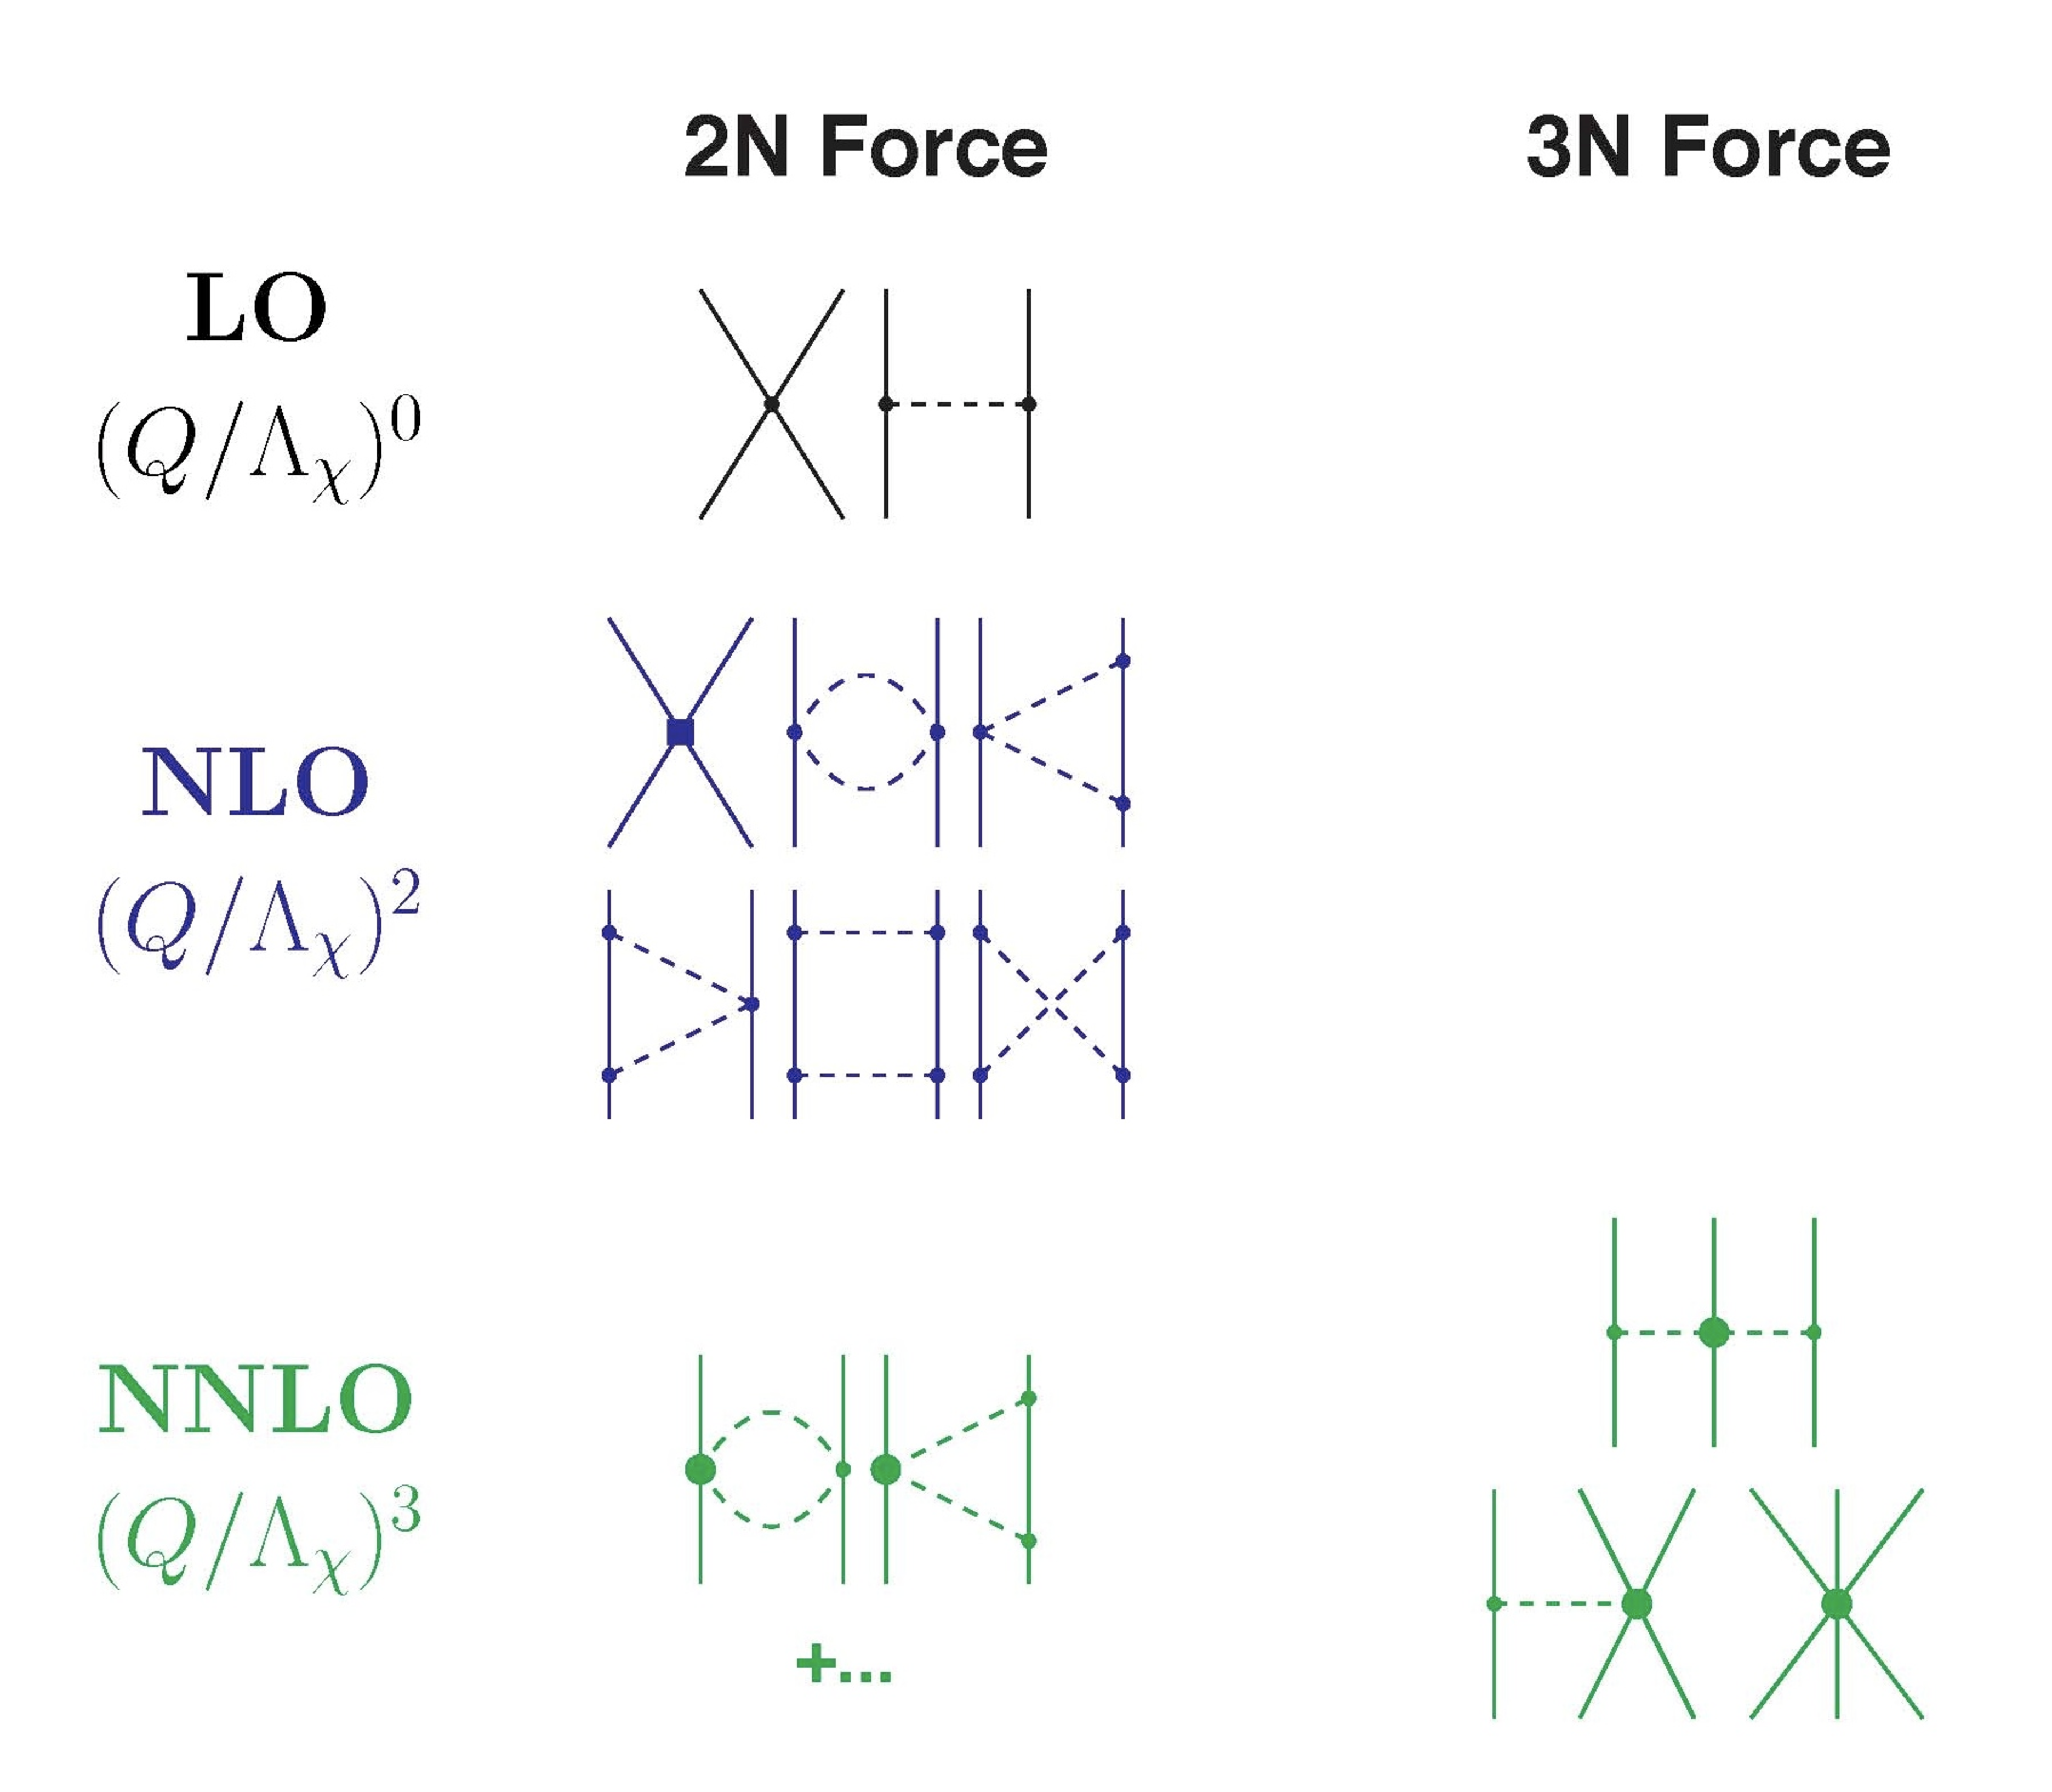
\includegraphics{Chapter8-figures/diagNNLO.pdf}}
%\vspace*{-1.0cm}
\caption{Nuclear forces in ChPT up to NNLO. Solid lines
represent nucleons and dashed lines pions. 
Small dots, large solid dots, and solid squares
denote vertices of index $\Delta_i= \, $ 0, 1, and 2, respectively.}
\label{fig_diagNNLO}
\end{figure}
For an irreducible $NN$ diagram (``two-nucleon potential'', $A=2$, $C=1$),
Eq.~(\ref{eq_nu}) collapses to
\begin{equation} 
\nu =  2L + \sum_i \Delta_i \, .  
\label{eq_nunn} 
\end{equation}
Thus, in terms of naive dimensional analysis or ``Weinberg counting'' \cite{weinberg1990,weinberg1991},
the various orders of the irreducible graphs which define the chiral 
$NN$ potential 
are given by (cf.\ Fig.~\ref{fig_diagNNLO})
\begin{eqnarray}
V_{\rm LO} & = & 
V_{\rm ct}^{(0)} + 
V_{1\pi}^{(0)} 
\label{eq_VLO}
\\
V_{\rm NLO} & = & V_{\rm LO} +
V_{\rm ct}^{(2)} + 
V_{1\pi}^{(2)} +
V_{2\pi}^{(2)} 
\label{eq_VNLO}
\\
V_{\rm NNLO} & = & V_{\rm NLO} +
V_{1\pi}^{(3)} + 
V_{2\pi}^{(3)} 
\label{eq_VNNLO}
\end{eqnarray}
where 
the superscript denotes the order $\nu$ of the low-momentum expansion.
LO stands for leading order, NLO for next-to-leading
order and NNLO stands for next-to-next-to leading order.
Contact potentials carry the subscript ``ct'' and
pion-exchange potentials can be identified by an obvious subscript.

The charge-independent one-pion-exchange (1PE) potential reads
\begin{equation}
V_{1\pi} ({\vec p}~', \vec p) = - 
%\frac{1}{(2\pi)^3} \,
\frac{g_A^2}{4f_\pi^2}
\: 
{\vec \tau}_1 \cdot {\vec \tau}_2 
\:
\frac{
\vec \sigma_1 \cdot \vec q \,\, \vec \sigma_2 \cdot \vec q}
{q^2 + m_\pi^2} 
\,,
\label{eq:eq_1PEci}
\end{equation}
where ${\vec p}~'$ and $\vec p$ designate the final and initial
nucleon momenta in the center-of-mass system (CMS) and $\vec q \equiv
{\vec p}~' - \vec p$ is the momentum transfer; $\vec \sigma_{1,2}$ and
$\vec tau_{1,2}$ are the spin and isospin operators of nucleon 1 and
2; $g_A$, $f_\pi$, and $m_\pi$ denote axial-vector coupling constant,
the pion decay constant, and the pion mass, respectively. As in Ref.~\cite{carlsson2014}, we use
$f_\pi=92.4$ MeV and $g_A=1.29$ throughout this work.  
Since higher order corrections contribute only to mass
and coupling constant renormalizations and since, on shell, there are
no relativistic corrections, the on-shell 1PE has the form
of Eq.~(\ref{eq:eq_1PEci}) to all orders.

It is well known that, for high-precision $NN$ potentials,
charge dependence is important.
Therefore, we will 
take the charge dependence of the 1PE into account.
Defining a pion-mass dependent 1PE by
\[
V_{1\pi} (m_\pi) \equiv - \,
%\frac{1}{(2\pi)^3} \,
\frac{g_A^2}{4f_\pi^2} \,
\frac{
\vec \sigma_1 \cdot \vec q \,\, \vec \sigma_2 \cdot \vec q}
{q^2 + m_\pi^2} 
\,,
\]
the 1PE for proton-proton ($pp$) and neutron-neutron ($nn$)
scattering is
\[
V_{1\pi}^{(pp)} ({\vec p}~', \vec p) = 
V_{1\pi}^{(nn)} ({\vec p}~', \vec p) =
V_{1\pi} (m_{\pi^0}) \,,
\]
while for neutron-proton ($np$) scattering we have
\[
V_{1\pi}^{(np)} ({\vec p}~', \vec p) 
= -V_{1\pi} (m_{\pi^0}) + (-1)^{T+1}\, 2\, V_{1\pi} (m_{\pi^\pm})
\,,
\]
where $T$ denotes the isospin of the two-nucleon system.
We use $m_{\pi^0}=134.9766$ MeV and
 $m_{\pi^\pm}=139.5702$ MeV.
For the leading-order, next-to-leading order and NNLO, we refer the reader to Refs.~\cite{machleidt2011,carlsson2014}.
The final interaction at order NNLO is multiplied with the following factors \cite{machleidt2011},
\begin{equation}
\widehat{V}({\vec p}~',{\vec p})
\equiv 
\frac{1}{(2\pi)^3}
\sqrt{\frac{M_N}{E_{p'}}}\:  
{V}({\vec p}~',{\vec p})\:
 \sqrt{\frac{M_N}{E_{p}}}
\label{eq_minrel1}
\end{equation}
with $E_p=\sqrt{M_N^2+p^2}$ and
where the factor $1/(2\pi)^3$ is just added for convenience.
The potential $\widehat{V}$ satisfies the nonrelativistic
Lippmann-Schwinger (LS) equation,
\begin{equation}
 \widehat{T}({\vec p}~',{\vec p})= \widehat{V}({\vec p}~',{\vec p})+
\int d^3p''\:
\widehat{V}({\vec p}~',{\vec p}~'')\:
\frac{M_N}
{{ p}^{2}-{p''}^{2}+i\epsilon}\:
\widehat{T}({\vec p}~'',{\vec p}) \, .
\label{eq_LS}
\end{equation}
In $pp$ scattering, we use $M_N=M_p=938.2720$ MeV,
and in $nn$ scattering, $M_N=M_n=939.5653$ MeV.
Moreover, the on-shell momentum is simply
\begin{equation}
p^2  =  \frac12 M_N T_{\rm lab} \,,
\end{equation}
where $T_{\rm lab}$ denotes 
the kinetic energy of the incident nucleon 
in the laboratory system (``Lab.\ Energy'').
For $np$ scattering, we have
\begin{eqnarray}
M_N  &=&  \frac{2M_pM_n}{M_p+M_n} = 938.9182 \mbox{ MeV, and}
\\
p^2 & = & \frac{M_p^2 T_{\rm lab} (T_{\rm lab} + 2M_n)}
               {(M_p + M_n)^2 + 2T_{\rm lab} M_p}  
\,,
\end{eqnarray}
which is based upon relativistic kinematics.

Iteration of $\widehat V$ in the LS equation, Eq.~(\ref{eq_LS}),
requires cutting $\widehat V$ off for high momenta to avoid infinities.
This is consistent with the fact that ChPT
is a low-momentum expansion which
is valid only for momenta $Q \ll \Lambda_\chi \approx 1$ GeV.
Therefore, the potential $\widehat V$
is multiplied
with the regulator function $f(p',p)$,
\begin{equation}
{\widehat V}(\vec{ p}~',{\vec p})
\longmapsto
{\widehat V}(\vec{ p}~',{\vec p}) \, f(p',p) 
\end{equation}
with
\begin{equation}
f(p',p) = \exp[-(p'/\Lambda)^{2n}-(p/\Lambda)^{2n}] \,.
\label{eq:eq_f}
\end{equation}


Up to NNLO in chiral perturbation theory there are, in addition to the
two-body interaction diagrams discussed above, also a few three-body
interaction diagrams, see Fig.~\ref{fig_diagNNLO}. In
chiral perturbation theory, the orders are generated systematically,
and at a given chiral order the number of Feynman diagrams is
finite. Consistency requires that a calculation includes all diagrams
which are present at the chosen order. In this work we employ 
chirally consistent many-body calculations including all NNLO nuclear
interactions.

There are in total five contact terms that determine the strength of the NNLO
three-nucleon force (3NF); $c_1,c_3,$ and $c_4$ are associated with
the three-body two-pion-exchange (2PE) diagram, $c_D$ and $c_E$
determine the strength of the one-pion-exchange plus contact (1PE)
diagram and the pure contact (CNT) diagram, respectively. Following
the notation of Ref.~\cite{epelbaum2002} the three-body diagrams are given
by
\begin{equation}
V^{\textnormal{2PE}}_{ijk} = \sum_{i \neq j \neq k} \frac{1}{2} \left( \frac{g_A}{f_{\pi}} \right)^2 \frac{(\vec{\sigma_i} \cdot \vec{q_i})(\vec{\sigma_j}\cdot \vec{q_j})}{(\vec{q_i}^2 + m_{\pi)}^2)(\vec{q_j}^2 + m_{\pi)}^2)} F_{ijk}^{\alpha \beta} \tau_i^{\alpha}\tau_{j}^{\beta} \,,
\end{equation}
where $q_{i}$ denotes the momentum transfer associated with nucleon $i$, and
\begin{align}
F_{ijk}^{\alpha \beta} ={}&  \delta^{\alpha \beta} \left[ -\frac{4c_1m_{\pi}^2}{f_{\pi}^2} + \frac{2c_3}{f_{\pi}^2}\vec{q_i}\cdot \vec{q_j}\right]\\
{}&+\sum_{\gamma}\frac{c_4}{f_{\pi}^2}\epsilon^{\alpha \beta \gamma} \tau_{k}^{\gamma} \vec{\sigma_k} \cdot [\vec{q_i} \times \vec{q_j}] \,.
\end{align}
For this diagram, no new parameters are introduced since the $c_1,c_3,c_4$ appear already in the 2PE two-nucleon interaction. The remaining two three-body terms are given by
\begin{equation}
V^{\textnormal{1PE}}_{ijk} = -\sum_{i \neq j \neq k} \frac{g_A}{8f_{\pi}^2} \frac{c_D}{f_{\pi}^2\Lambda_{\chi}} \frac{ (\vec{\sigma_j} \cdot \vec{q_j})}{(\vec{q_j}^2 + m_{\pi}^2)} (\tau_i \cdot \tau_j)(\vec{\sigma_i}\cdot \vec{\sigma_j})
\end{equation}
and
\begin{equation}
V^{\textnormal{CNT}}_{ijk} = \frac{1}{2}\sum_{i \neq j \neq k} \frac{c_E}{f_{\pi}^4 \Lambda_{\chi}} (\tau_i \cdot \tau_j) 
\end{equation}
with $\Lambda_{\chi}=700$ MeV. Following~\cite{navratil2007}, we use a regulator depending on the momentum-transfer $q$, 
\begin{equation}
f(q) = \exp[-q^4/\Lambda]
\end{equation}
and thus obtain a local three-body force. 




\section{Hartree-Fock theory}

Hartree-Fock (HF) theory is an algorithm for finding an approximative
expression for the ground state of a given Hamiltonian. The basic
ingredients are Define a single-particle basis $\{\psi_{\alpha}\}$ so
that
\[ 
\hat{h}^{\mathrm{HF}}\psi_{\alpha} = \varepsilon_{\alpha}\psi_{\alpha}
\]
with the Hartree-Fock Hamiltonian defined as
\[
\hat{h}^{\mathrm{HF}}=\hat{t}+\hat{u}_{\mathrm{ext}}+\hat{u}^{\mathrm{HF}}
\]

The term $\hat{u}^{\mathrm{HF}}$ is a single-particle potential to be
determined by the HF algorithm.

The HF algorithm means to choose $\hat{u}^{\mathrm{HF}}$ in order to
have
\[ \langle \hat{H} \rangle = E^{\mathrm{HF}}= \langle \Phi_0 | \hat{H}|\Phi_0 \rangle
\]
that is to find a local minimum with a Slater determinant $\Phi_0$
being the ansatz for the ground state.  The variational principle
ensures that $E^{\mathrm{HF}} \ge E_0$, with $E_0$ the exact ground
state energy.

We will show that the Hartree-Fock Hamiltonian $\hat{h}^{\mathrm{HF}}$
equals our definition of the operator $\hat{f}$ discussed in
connection with the new definition of the normal-ordered Hamiltonian
(see later lectures), that is we have, for a specific matrix element
\[
\langle p |\hat{h}^{\mathrm{HF}}| q \rangle =\langle p |\hat{f}| q \rangle=\langle p|\hat{t}+\hat{u}_{\mathrm{ext}}|q \rangle +\sum_{i\le F} \langle pi | \hat{V} | qi\rangle_{AS},
\]
meaning that
\[
\langle p|\hat{u}^{\mathrm{HF}}|q\rangle = \sum_{i\le F} \langle pi | \hat{V} | qi\rangle_{AS}.
\]
The so-called Hartree-Fock potential $\hat{u}^{\mathrm{HF}}$ brings an
explicit medium dependence due to the summation over all
single-particle states below the Fermi level $F$. It brings also in an
explicit dependence on the two-body interaction (in nuclear physics we
can also have complicated three- or higher-body forces). The two-body
interaction, with its contribution from the other bystanding fermions,
creates an effective mean field in which a given fermion moves, in
addition to the external potential $\hat{u}_{\mathrm{ext}}$ which
confines the motion of the fermion. For systems like nuclei, there is
no external confining potential. Nuclei are examples of self-bound
systems, where the binding arises due to the intrinsic nature of the
strong force. For nuclear systems thus, there would be no external
one-body potential in the Hartree-Fock Hamiltonian.


Another possibility is to expand the single-particle functions in a
known basis and vary the coefficients, that is, the new
single-particle wave function is written as a linear expansion in
terms of a fixed chosen orthogonal basis (for example the well-known
harmonic oscillator functions or the hydrogen-like functions etc).  We
define our new Hartree-Fock single-particle basis by performing a
unitary transformation on our previous basis (labelled with greek
indices) as
\begin{equation}
\psi_p^{HF}  = \sum_{\lambda} C_{p\lambda}\phi_{\lambda}. \label{eq:newbasis}
\end{equation}
In this case we vary the coefficients $C_{p\lambda}$. If the basis has
infinitely many solutions, we need to truncate the above sum.  We
assume that the basis $\phi_{\lambda}$ is orthogonal. A unitary
transformation keeps the orthogonality, as discussed in exercise 1
below.




It is normal to choose a single-particle basis defined as the
eigenfunctions of parts of the full Hamiltonian. The typical situation
consists of the solutions of the one-body part of the Hamiltonian,
that is we have
\[
\hat{h}_0\phi_{\lambda}=\epsilon_{\lambda}\phi_{\lambda}.
\]
The single-particle wave functions $\phi_{\lambda}({\bf r})$, defined
by the quantum numbers $\lambda$ and ${\bf r}$ are defined as the
overlap
\[
   \phi_{\lambda}({\bf r})  = \langle {\bf r} | \lambda \rangle .
\]




In our discussions hereafter we will use our definitions of
single-particle states above and below the Fermi ($F$) level given by
the labels $ijkl\dots \le F$ for so-called single-hole states and
$abcd\dots > F$ for so-called particle states.  For general
single-particle states we employ the labels $pqrs\dots$.





\[
  E[\Phi] = \sum_{\mu=1}^A \langle \mu | h | \mu \rangle
  + \frac{1}{2}\sum_{{\mu}=1}^A\sum_{{\nu}=1}^A \langle \mu\nu|\hat{v}|\mu\nu\rangle_{AS},
\]
we found the expression for the energy functional in terms of the
basis function $\phi_{\lambda}({\bf r})$. We then varied the above
energy functional with respect to the basis functions $|\mu \rangle$.
Now we are interested in defining a new basis defined in terms of a
chosen basis as defined in Eq.~(\ref{eq:newbasis}). We can then rewrite
the energy functional as
\begin{equation}
  E[\Phi^{HF}] 
  = \sum_{i=1}^A \langle i | h | i \rangle +
  \frac{1}{2}\sum_{ij=1}^A\langle ij|\hat{v}|ij\rangle_{AS}, \label{FunctionalEPhi2}
\end{equation}
where $\Phi^{HF}$ is the new Slater determinant defined by the new
basis of Eq.~(\ref{eq:newbasis}).





Using Eq.~(\ref{eq:newbasis}) we can rewrite
Eq.~(\ref{FunctionalEPhi2}) as
\begin{equation}
  E[\Psi] 
  = \sum_{i=1}^A \sum_{\alpha\beta} C^*_{i\alpha}C_{i\beta}\langle \alpha | h | \beta \rangle +
  \frac{1}{2}\sum_{ij=1}^A\sum_{{\alpha\beta\gamma\delta}} C^*_{i\alpha}C^*_{j\beta}C_{i\gamma}C_{j\delta}\langle \alpha\beta|\hat{v}|\gamma\delta\rangle_{AS}. \label{FunctionalEPhi3}
\end{equation}


We wish now to minimize the above functional. We introduce again a set
of Lagrange multipliers, noting that since $\langle i | j \rangle
= \delta_{i,j}$ and $\langle \alpha | \beta \rangle
= \delta_{\alpha,\beta}$, the coefficients $C_{i\gamma}$ obey the
relation
\[
 \langle i | j \rangle=\delta_{i,j}=\sum_{\alpha\beta} C^*_{i\alpha}C_{i\beta}\langle \alpha | \beta \rangle=
\sum_{\alpha} C^*_{i\alpha}C_{i\alpha},
\]
which allows us to define a functional to be minimized that reads
\begin{equation}
  F[\Phi^{HF}]=E[\Phi^{HF}] - \sum_{i=1}^A\epsilon_i\sum_{\alpha} C^*_{i\alpha}C_{i\alpha}.
\end{equation}







Minimizing with respect to $C^*_{i\alpha}$, remembering that the
equations for $C^*_{i\alpha}$ and $C_{i\alpha}$ can be written as two
independent equations, we obtain
\[
\frac{d}{dC^*_{i\alpha}}\left[  E[\Phi^{HF}] - \sum_{j}\epsilon_j\sum_{\alpha} C^*_{j\alpha}C_{j\alpha}\right]=0,
\]
which yields for every single-particle state $i$ and index $\alpha$
(recalling that the coefficients $C_{i\alpha}$ are matrix elements of
a unitary (or orthogonal for a real symmetric matrix) matrix) the
following Hartree-Fock equations
\[
\sum_{\beta} C_{i\beta}\langle \alpha | h | \beta \rangle+
\sum_{j=1}^A\sum_{\beta\gamma\delta} C^*_{j\beta}C_{j\delta}C_{i\gamma}\langle \alpha\beta|\hat{v}|\gamma\delta\rangle_{AS}=\epsilon_i^{HF}C_{i\alpha}.
\]


We can rewrite this equation as (changing dummy variables)
\[
\sum_{\beta} \left\{\langle \alpha | h | \beta \rangle+
\sum_{j}^A\sum_{\gamma\delta} C^*_{j\gamma}C_{j\delta}\langle \alpha\gamma|\hat{v}|\beta\delta\rangle_{AS}\right\}C_{i\beta}=\epsilon_i^{HF}C_{i\alpha}.
\]
Note that the sums over greek indices run over the number of basis set
functions (in principle an infinite number).





Defining 
\[
h_{\alpha\beta}^{HF}=\langle \alpha | h | \beta \rangle+
\sum_{j=1}^A\sum_{\gamma\delta} C^*_{j\gamma}C_{j\delta}\langle \alpha\gamma|\hat{v}|\beta\delta\rangle_{AS},
\]
we can rewrite the new equations as 
\begin{equation}
\sum_{\gamma}h_{\alpha\beta}^{HF}C_{i\beta}=\epsilon_i^{HF}C_{i\alpha}. \label{eq:newhf}
\end{equation}
The latter is nothing but a standard eigenvalue problem. Compared with
Eq.~(\ref{eq:hartreefockcoordinatespace}), we see that we do not need
to compute any integrals in an iterative procedure for solving the
equations.  It suffices to tabulate the matrix elements
$\langle \alpha | h | \beta \rangle$ and
$\langle \alpha\gamma|\hat{v}|\beta\delta\rangle_{AS}$ once and for
all. Successive iterations require thus only a look-up in tables over
one-body and two-body matrix elements. These details will be discussed
below when we solve the Hartree-Fock equations numerical.


Our Hartree-Fock matrix is thus
\[
\hat{h}_{\alpha\beta}^{HF}=\langle \alpha | \hat{h}_0 | \beta \rangle+
\sum_{j=1}^A\sum_{\gamma\delta} C^*_{j\gamma}C_{j\delta}\langle \alpha\gamma|\hat{v}|\beta\delta\rangle_{AS}.
\]
The Hartree-Fock equations are solved in an iterative waym starting
with a guess for the coefficients $C_{j\gamma}=\delta_{j,\gamma}$ and
solving the equations by diagonalization till the new single-particle
energies $\epsilon_i^{\mathrm{HF}}$ do not change anymore by a
prefixed quantity.




Normally we assume that the single-particle basis $|\beta\rangle$
forms an eigenbasis for the operator $\hat{h}_0$, meaning that the
Hartree-Fock matrix becomes
\[
\hat{h}_{\alpha\beta}^{HF}=\epsilon_{\alpha}\delta_{\alpha,\beta}+
\sum_{j=1}^A\sum_{\gamma\delta} C^*_{j\gamma}C_{j\delta}\langle \alpha\gamma|\hat{v}|\beta\delta\rangle_{AS}.
\]
The Hartree-Fock eigenvalue problem
\[
\sum_{\beta}\hat{h}_{\alpha\beta}^{HF}C_{i\beta}=\epsilon_i^{\mathrm{HF}}C_{i\alpha},
\]
can be written out in a more compact form as
\[
\hat{h}^{HF}\hat{C}=\epsilon^{\mathrm{HF}}\hat{C}. 
\]




The Hartree-Fock equations are, in their simplest form, solved in an
iterative way, starting with a guess for the coefficients
$C_{i\alpha}$. We label the coefficients as $C_{i\alpha}^{(n)}$, where
the subscript $n$ stands for iteration $n$.  To set up the algorithm
we can proceed as follows:

We start with a guess
$C_{i\alpha}^{(0)}=\delta_{i,\alpha}$. Alternatively, we could have
used random starting values as long as the vectors are
normalized. Another possibility is to give states below the Fermi
level a larger weight.  The Hartree-Fock matrix simplifies then to
(assuming that the coefficients $C_{i\alpha} $ are real)
\[
\hat{h}_{\alpha\beta}^{HF}=\epsilon_{\alpha}\delta_{\alpha,\beta}+
\sum_{j = 1}^A\sum_{\gamma\delta} C_{j\gamma}^{(0)}C_{j\delta}^{(0)}\langle \alpha\gamma|\hat{v}|\beta\delta\rangle_{AS}.
\]




Solving the Hartree-Fock eigenvalue problem yields then new
eigenvectors $C_{i\alpha}^{(1)}$ and eigenvalues $\epsilon_i^{HF(1)}$.
With the new eigenvalues we can set up a new Hartree-Fock potential
\[
\sum_{j = 1}^A\sum_{\gamma\delta} C_{j\gamma}^{(1)}C_{j\delta}^{(1)}\langle \alpha\gamma|\hat{v}|\beta\delta\rangle_{AS}.
\]
The diagonalization with the new Hartree-Fock potential yields new
eigenvectors and eigenvalues.  This process is continued till for
example
\[
\frac{\sum_{p} |\epsilon_i^{(n)}-\epsilon_i^{(n-1)}|}{m} \le \lambda,  
\]
where $\lambda$ is a user prefixed quantity ($\lambda \sim 10^{-8}$ or
smaller) and $p$ runs over all calculated single-particle energies and
$m$ is the number of single-particle states.


We can rewrite the ground state energy by adding and subtracting
$\hat{u}^{HF}(x_i)$
\[
  E_0^{HF} =\langle \Phi_0 | \hat{H} | \Phi_0\rangle = 
\sum_{i\le F}^A \langle i | \hat{h}_0 +\hat{u}^{HF}| j\rangle+ \frac{1}{2}\sum_{i\le F}^A\sum_{j \le F}^A\left[\langle ij |\hat{v}|ij \rangle-\langle ij|\hat{v}|ji\rangle\right]-\sum_{i\le F}^A \langle i |\hat{u}^{HF}| i\rangle,
\]
which results in
\[
  E_0^{HF}
  = \sum_{i\le F}^A \varepsilon_i^{HF} + \frac{1}{2}\sum_{i\le F}^A\sum_{j \le F}^A\left[\langle ij |\hat{v}|ij \rangle-\langle ij|\hat{v}|ji\rangle\right]-\sum_{i\le F}^A \langle i |\hat{u}^{HF}| i\rangle.
\]
Our single-particle states $ijk\dots$ are now single-particle states
obtained from the solution of the Hartree-Fock equations.



Using our definition of the Hartree-Fock single-particle energies we
obtain then the following expression for the total ground-state energy
\[
  E_0^{HF}
  = \sum_{i\le F}^A \varepsilon_i - \frac{1}{2}\sum_{i\le F}^A\sum_{j \le F}^A\left[\langle ij |\hat{v}|ij \rangle-\langle ij|\hat{v}|ji\rangle\right].
\]


\section{Full Configuration Interaction Theory}

We have defined the ansatz for the ground state as 
\[
|\Phi_0\rangle = \left(\prod_{i\le F}\hat{a}_{i}^{\dagger}\right)|0\rangle,
\]
where the index $i$ defines different single-particle states up to the Fermi level. We have assumed that we have $N$ fermions. 
A given one-particle-one-hole ($1p1h$) state can be written as
\[
|\Phi_i^a\rangle = \hat{a}_{a}^{\dagger}\hat{a}_i|\Phi_0\rangle,
\]
while a $2p2h$ state can be written as
\[
|\Phi_{ij}^{ab}\rangle = \hat{a}_{a}^{\dagger}\hat{a}_{b}^{\dagger}\hat{a}_j\hat{a}_i|\Phi_0\rangle,
\]
and a general $ApAh$ state as 
\[
|\Phi_{ijk\dots}^{abc\dots}\rangle = \hat{a}_{a}^{\dagger}\hat{a}_{b}^{\dagger}\hat{a}_{c}^{\dagger}\dots\hat{a}_k\hat{a}_j\hat{a}_i|\Phi_0\rangle.
\]

We use letters $ijkl\dots$ for states below the Fermi level and $abcd\dots$ for states above the Fermi level. A general single-particle state is given by letters $pqrs\dots$.

We can then expand our exact state function for the ground state 
as
\[
|\Psi_0\rangle=C_0|\Phi_0\rangle+\sum_{ai}C_i^a|\Phi_i^a\rangle+\sum_{abij}C_{ij}^{ab}|\Phi_{ij}^{ab}\rangle+\dots
=(C_0+\hat{C})|\Phi_0\rangle,
\]
where we have introduced the so-called correlation operator 
\[
\hat{C}=\sum_{ai}C_i^a\hat{a}_{a}^{\dagger}\hat{a}_i  +\sum_{abij}C_{ij}^{ab}\hat{a}_{a}^{\dagger}\hat{a}_{b}^{\dagger}\hat{a}_j\hat{a}_i+\dots
\]
Since the normalization of $\Psi_0$ is at our disposal and since $C_0$ is by hypothesis non-zero, we may arbitrarily set $C_0=1$ with 
corresponding proportional changes in all other coefficients. Using this so-called intermediate normalization we have
\[
\langle \Psi_0 | \Phi_0 \rangle = \langle \Phi_0 | \Phi_0 \rangle = 1, 
\]
resulting in 
\[
|\Psi_0\rangle=(1+\hat{C})|\Phi_0\rangle.
\]


We rewrite 
\[
|\Psi_0\rangle=C_0|\Phi_0\rangle+\sum_{ai}C_i^a|\Phi_i^a\rangle+\sum_{abij}C_{ij}^{ab}|\Phi_{ij}^{ab}\rangle+\dots,
\]
in a more compact form as 
\[
|\Psi_0\rangle=\sum_{PH}C_H^P\Phi_H^P=\left(\sum_{PH}C_H^P\hat{A}_H^P\right)|\Phi_0\rangle,
\]
where $H$ stands for $0,1,\dots,n$ hole states and $P$ for $0,1,\dots,n$ particle states. 
Our requirement of unit normalization gives
\[
\langle \Psi_0 | \Psi_0 \rangle = \sum_{PH}|C_H^P|^2= 1,
\]
and the energy can be written as 
\[
E= \langle \Psi_0 | \hat{H} |\Psi_0 \rangle= \sum_{PP'HH'}C_H^{*P}\langle \Phi_H^P | \hat{H} |\Phi_{H'}^{P'} \rangle C_{H'}^{P'}.
\]


Normally 
\[
E= \langle \Psi_0 | \hat{H} |\Psi_0 \rangle= \sum_{PP'HH'}C_H^{*P}\langle \Phi_H^P | \hat{H} |\Phi_{H'}^{P'} \rangle C_{H'}^{P'},
\]
is solved by diagonalization setting up the Hamiltonian matrix defined by the basis of all possible Slater determinants. A diagonalization
is equivalent to finding the variational minimum   of 
\[
 \langle \Psi_0 | \hat{H} |\Psi_0 \rangle-\lambda \langle \Psi_0 |\Psi_0 \rangle,
\]
where $\lambda$ is a variational multiplier to be identified with the energy of the system.

The minimization process results in 
\[
\delta\left[ \langle \Psi_0 | \hat{H} |\Psi_0 \rangle-\lambda \langle \Psi_0 |\Psi_0 \rangle\right]=
\]
\[
\sum_{P'H'}\left\{\delta[C_H^{*P}]\langle \Phi_H^P | \hat{H} |\Phi_{H'}^{P'} \rangle C_{H'}^{P'}+
C_H^{*P}\langle \Phi_H^P | \hat{H} |\Phi_{H'}^{P'} \rangle \delta[C_{H'}^{P'}]-
\lambda( \delta[C_H^{*P}]C_{H'}^{P'}+C_H^{*P}\delta[C_{H'}^{P'}]\right\} = 0.
\]
Since the coefficients $\delta[C_H^{*P}]$ and $\delta[C_{H'}^{P'}]$ are complex conjugates it is necessary and sufficient to require the quantities that multiply with $\delta[C_H^{*P}]$ to vanish.  

This leads to 
\[
\sum_{P'H'}\langle \Phi_H^P | \hat{H} |\Phi_{H'}^{P'} \rangle C_{H'}^{P'}-\lambda C_H^{P}=0,
\]
for all sets of $P$ and $H$.

If we then multiply by the corresponding $C_H^{*P}$ and sum over $PH$ we obtain
\[ 
\sum_{PP'HH'}C_H^{*P}\langle \Phi_H^P | \hat{H} |\Phi_{H'}^{P'} \rangle C_{H'}^{P'}-\lambda\sum_{PH}|C_H^P|^2=0,
\]
leading to the identification $\lambda = E$. This means that we have for all $PH$ sets
\begin{equation}
\sum_{P'H'}\langle \Phi_H^P | \hat{H} -E|\Phi_{H'}^{P'} \rangle = 0. \label{eq:fullci}
\end{equation}



An alternative way to derive the last equation is to start from 
\[
(\hat{H} -E)|\Psi_0\rangle = (\hat{H} -E)\sum_{P'H'}C_{H'}^{P'}|\Phi_{H'}^{P'} \rangle=0, 
\]
and if this equation is successively projected against all $\Phi_H^P$ in the expansion of $\Psi$, we end up with Eq.~(\ref{eq:fullci}).

One solves this equation normally by diagonalization. If we are able to solve this equation exactly (that is
numerically exactly) in a large Hilbert space (it will be truncated in terms of the number of single-particle states included in the definition
of Slater determinants), it can then serve as a benchmark for other many-body methods which approximate the correlation operator
$\hat{C}$.  


\subsection{Example of a Hamiltonian matrix}

Suppose, as an example, that we have six fermions below the Fermi level.
This means that we can make at most $6p-6h$ excitations. If we have an infinity of single particle states above the Fermi level, we will obviously have an infinity of say $2p-2h$ excitations. Each such way to configure the particles is called a \textbf{configuration}. We will always have to truncate in the basis of single-particle states.
This gives us a finite number of possible Slater determinants. Our Hamiltonian matrix would then look like (where each block can have a large dimensionalities):

\begin{table}
\begin{center}
\begin{tabular}{cccccccc}
\hline
\multicolumn{1}{c}{  } & \multicolumn{1}{c}{ $0p-0h$ } & \multicolumn{1}{c}{ $1p-1h$ } & \multicolumn{1}{c}{ $2p-2h$ } & \multicolumn{1}{c}{ $3p-3h$ } & \multicolumn{1}{c}{ $4p-4h$ } & \multicolumn{1}{c}{ $5p-5h$ } & \multicolumn{1}{c}{ $6p-6h$ } \\
\hline
$0p-0h$ & x       & x       & x       & 0       & 0       & 0       & 0       \\
$1p-1h$ & x       & x       & x       & x       & 0       & 0       & 0       \\
$2p-2h$ & x       & x       & x       & x       & x       & 0       & 0       \\
$3p-3h$ & 0       & x       & x       & x       & x       & x       & 0       \\
$4p-4h$ & 0       & 0       & x       & x       & x       & x       & x       \\
$5p-5h$ & 0       & 0       & 0       & x       & x       & x       & x       \\
$6p-6h$ & 0       & 0       & 0       & 0       & x       & x       & x       \\
\hline
\end{tabular}
\end{center}
\end{table}
with a two-body force. Why are there non-zero blocks of elements? 
If we use a Hartree-Fock basis, this corresponds to a particular unitary transformation where matrix elements of the type $\langle 0p-0h \vert \hat{H} \vert 1p-1h\rangle =\langle \Phi_0 | \hat{H}|\Phi_{i}^{a}\rangle=0$ and our Hamiltonian matrix becomes 

\begin{table}
\begin{center}
\begin{tabular}{cccccccc}
\hline
\multicolumn{1}{c}{  } & \multicolumn{1}{c}{ $0p-0h$ } & \multicolumn{1}{c}{ $1p-1h$ } & \multicolumn{1}{c}{ $2p-2h$ } & \multicolumn{1}{c}{ $3p-3h$ } & \multicolumn{1}{c}{ $4p-4h$ } & \multicolumn{1}{c}{ $5p-5h$ } & \multicolumn{1}{c}{ $6p-6h$ } \\
\hline
$0p-0h$ & $\tilde{x}$ & 0           & $\tilde{x}$ & 0           & 0           & 0           & 0           \\
$1p-1h$ & 0           & $\tilde{x}$ & $\tilde{x}$ & $\tilde{x}$ & 0           & 0           & 0           \\
$2p-2h$ & $\tilde{x}$ & $\tilde{x}$ & $\tilde{x}$ & $\tilde{x}$ & $\tilde{x}$ & 0           & 0           \\
$3p-3h$ & 0           & $\tilde{x}$ & $\tilde{x}$ & $\tilde{x}$ & $\tilde{x}$ & $\tilde{x}$ & 0           \\
$4p-4h$ & 0           & 0           & $\tilde{x}$ & $\tilde{x}$ & $\tilde{x}$ & $\tilde{x}$ & $\tilde{x}$ \\
$5p-5h$ & 0           & 0           & 0           & $\tilde{x}$ & $\tilde{x}$ & $\tilde{x}$ & $\tilde{x}$ \\
$6p-6h$ & 0           & 0           & 0           & 0           & $\tilde{x}$ & $\tilde{x}$ & $\tilde{x}$ \\
\hline
\end{tabular}
\end{center}
\end{table}
If we do not make any truncations in the possible sets of Slater determinants (many-body states) we can make by distributing $A$ nucleons among $n$ single-particle states, we call such a calculation for 
\begin{itemize}
\item Full configuration interaction theory
\end{itemize}

\noindent
If we make truncations, we have different possibilities

\begin{itemize}
\item The standard nuclear shell-model. Here we define an effective Hilbert space with respect to a given core. The calculations are normally then performed for all many-body states that can be constructed from the effective Hilbert spaces. This approach requires a properly defined effective Hamiltonian

\item We can truncate in the number of excitations. For example, we can limit the possible Slater determinants to only $1p-1h$ and $2p-2h$ excitations. This is called a configuration interaction calculation at the level of singles and doubles excitations, or just CISD. 

\item We can limit the number of excitations in terms of the excitation energies. If we do not define a core, this defines normally what is called the no-core shell-model approach. 
\end{itemize}

\noindent
What happens if we have a three-body interaction and a Hartree-Fock basis? 

Full configuration interaction theory calculations provide in principle, if we can diagonalize numerically, all states of interest. The dimensionality of the problem explodes however quickly.

The total number of Slater determinants which can be built with say $N$ neutrons distributed among $n$ single particle states is
\[
\left (\begin{array}{c} n \\ N\end{array} \right) =\frac{n!}{(n-N)!N!}. 
\]

For a model space which comprises the first for major shells only $0s$, $0p$, $1s0d$ and $1p0f$ we have $40$ single particle states for neutrons and protons.  For the eight neutrons of oxygen-16 we would then have
\[
\left (\begin{array}{c} 40 \\ 8\end{array} \right) =\frac{40!}{(32)!8!}\sim 10^{9}, 
\]
and multiplying this with the number of proton Slater determinants we end up with approximately witha dimensionality $d$ of $d\sim 10^{18}$.


This number can be reduced if we look at specific symmetries only. However, the dimensionality explodes quickly!

\begin{itemize}
\item For Hamiltonian matrices of dimensionalities  which are smaller than $d\sim 10^5$, we would use so-called direct methods for diagonalizing the Hamiltonian matrix

\item For larger dimensionalities iterative eigenvalue solvers like Lanczos' method are used. The most efficient codes at present can handle matrices of $d\sim 10^{10}$. 
\end{itemize}

\noindent
\subsection{A non-practical way of solving the eigenvalue problem}

For reasons to come (links with Coupled-Cluster theory and Many-Body perturbation theory), 
we will rewrite Eq.~(\ref{eq:fullci}) as a set of coupled non-linear equations in terms of the unknown coefficients $C_H^P$. 
To obtain the eigenstates and eigenvalues in terms of non-linear equations is not a very practical approach. However, it serves the scope of linking FCI theory with approximative solutions to the many-body problem.

To see this, we look at the contributions arising from 
\[
\langle \Phi_H^P | = \langle \Phi_0|
\]
in  Eq.~(\ref{eq:fullci}), that is we multiply with $\langle \Phi_0 |$
from the left in 
\[
(\hat{H} -E)\sum_{P'H'}C_{H'}^{P'}|\Phi_{H'}^{P'} \rangle=0. 
\]
If we assume that we have a two-body operator at most, Slater's rule gives then an equation for the 
correlation energy in terms of $C_i^a$ and $C_{ij}^{ab}$ only.  We get then
\[
\langle \Phi_0 | \hat{H} -E| \Phi_0\rangle + \sum_{ai}\langle \Phi_0 | \hat{H} -E|\Phi_{i}^{a} \rangle C_{i}^{a}+
\sum_{abij}\langle \Phi_0 | \hat{H} -E|\Phi_{ij}^{ab} \rangle C_{ij}^{ab}=0,
\]
or 
\[
E-E_0 =\Delta E=\sum_{ai}\langle \Phi_0 | \hat{H}|\Phi_{i}^{a} \rangle C_{i}^{a}+
\sum_{abij}\langle \Phi_0 | \hat{H}|\Phi_{ij}^{ab} \rangle C_{ij}^{ab},
\]
where the energy $E_0$ is the reference energy and $\Delta E$ defines the so-called correlation energy.
The single-particle basis functions  could be the results of a Hartree-Fock calculation or just the eigenstates of the non-interacting part of the Hamiltonian. 

In our notes on Hartree-Fock calculations, 
we have already computed the matrix $\langle \Phi_0 | \hat{H}|\Phi_{i}^{a}\rangle $ and $\langle \Phi_0 | \hat{H}|\Phi_{ij}^{ab}\rangle$.  If we are using a Hartree-Fock basis, then the matrix elements
$\langle \Phi_0 | \hat{H}|\Phi_{i}^{a}\rangle=0$ and we are left with a \emph{correlation energy} given by
\[
E-E_0 =\Delta E^{HF}=\sum_{abij}\langle \Phi_0 | \hat{H}|\Phi_{ij}^{ab} \rangle C_{ij}^{ab}. 
\]


Inserting the various matrix elements we can rewrite the previous equation as
\[
\Delta E=\sum_{ai}\langle i| \hat{f}|a \rangle C_{i}^{a}+
\sum_{abij}\langle ij | \hat{v}| ab \rangle C_{ij}^{ab}.
\]
This equation determines the correlation energy but not the coefficients $C$. 
We need more equations. Our next step is to set up
\[
\langle \Phi_i^a | \hat{H} -E| \Phi_0\rangle + \sum_{bj}\langle \Phi_i^a | \hat{H} -E|\Phi_{j}^{b} \rangle C_{j}^{b}+
\sum_{bcjk}\langle \Phi_i^a | \hat{H} -E|\Phi_{jk}^{bc} \rangle C_{jk}^{bc}+
\sum_{bcdjkl}\langle \Phi_i^a | \hat{H} -E|\Phi_{jkl}^{bcd} \rangle C_{jkl}^{bcd}=0,
\]
as this equation will allow us to find an expression for the coefficents $C_i^a$ since we can rewrite this equation as 
\[
\langle i | \hat{f}| a\rangle +\langle \Phi_i^a | \hat{H}|\Phi_{i}^{a} \rangle C_{i}^{a}+ \sum_{bj\ne ai}\langle \Phi_i^a | \hat{H}|\Phi_{j}^{b} \rangle C_{j}^{b}+
\sum_{bcjk}\langle \Phi_i^a | \hat{H}|\Phi_{jk}^{bc} \rangle C_{jk}^{bc}+
\sum_{bcdjkl}\langle \Phi_i^a | \hat{H}|\Phi_{jkl}^{bcd} \rangle C_{jkl}^{bcd}=EC_i^a.
\]

We see that on the right-hand side we have the energy $E$. This leads to a non-linear equation in the unknown coefficients. 
These equations are normally solved iteratively ( that is we can start with a guess for the coefficients $C_i^a$). A common choice is to use perturbation theory for the first guess, setting thereby
\[
 C_{i}^{a}=\frac{\langle i | \hat{f}| a\rangle}{\epsilon_i-\epsilon_a}.
\]

The observant reader will however see that we need an equation for $C_{jk}^{bc}$ and $C_{jkl}^{bcd}$ as well.
To find equations for these coefficients we need then to continue our multiplications from the left with the various
$\Phi_{H}^P$ terms. 


For $C_{jk}^{bc}$ we need then
\[
\langle \Phi_{ij}^{ab} | \hat{H} -E| \Phi_0\rangle + \sum_{kc}\langle \Phi_{ij}^{ab} | \hat{H} -E|\Phi_{k}^{c} \rangle C_{k}^{c}+
\]
\[
\sum_{cdkl}\langle \Phi_{ij}^{ab} | \hat{H} -E|\Phi_{kl}^{cd} \rangle C_{kl}^{cd}+\sum_{cdeklm}\langle \Phi_{ij}^{ab} | \hat{H} -E|\Phi_{klm}^{cde} \rangle C_{klm}^{cde}+\sum_{cdefklmn}\langle \Phi_{ij}^{ab} | \hat{H} -E|\Phi_{klmn}^{cdef} \rangle C_{klmn}^{cdef}=0,
\]
and we can isolate the coefficients $C_{kl}^{cd}$ in a similar way as we did for the coefficients $C_{i}^{a}$. 
A standard choice for the first iteration is to set 
\[
C_{ij}^{ab} =\frac{\langle ij \vert \hat{v} \vert ab \rangle}{\epsilon_i+\epsilon_j-\epsilon_a-\epsilon_b}.
\]
At the end we can rewrite our solution of the Schroedinger equation in terms of $n$ coupled equations for the coefficients $C_H^P$.
This is a very cumbersome way of solving the equation. However, by using this iterative scheme we can illustrate how we can compute the
various terms in the wave operator or correlation operator $\hat{C}$. We will later identify the calculation of the various terms $C_H^P$
as parts of different many-body approximations to full CI. In particular, we can  relate this non-linear scheme with Coupled Cluster theory and
many-body perturbation theory.


\subsection{Summarizing FCI and bringing in approximative methods}


If we can diagonalize large matrices, FCI is the method of choice since:
\begin{itemize}
\item It gives all eigenvalues, ground state and excited states

\item The eigenvectors are obtained directly from the coefficients $C_H^P$ which result from the diagonalization

\item We can compute easily expectation values of other operators, as well as transition probabilities

\item Correlations are easy to understand in terms of contributions to a given operator beyond the Hartree-Fock contribution. This is the standard approach in  many-body theory. 
\end{itemize}

\noindent
The correlation energy is defined as, with a two-body Hamiltonian,  
\[
\Delta E=\sum_{ai}\langle i| \hat{f}|a \rangle C_{i}^{a}+
\sum_{abij}\langle ij | \hat{v}| ab \rangle C_{ij}^{ab}.
\]

The coefficients $C$ result from the solution of the eigenvalue problem. 
The energy of say the ground state is then
\[
E=E_{ref}+\Delta E,
\]
where the so-called reference energy is the energy we obtain from a Hartree-Fock calculation, that is
\[
E_{ref}=\langle \Phi_0 \vert \hat{H} \vert \Phi_0 \rangle.
\]

However, as we have seen, even for a small case like the four first major shells and a nucleus like oxygen-16, the dimensionality becomes quickly intractable. If we wish to include single-particle states that reflect weakly bound systems, we need a much larger single-particle basis. We need thus approximative methods that sum specific correlations to infinite order. 

Popular methods are
\begin{itemize}
\item Many-body perturbation theory (in essence a Taylor expansion)

\item Coupled cluster theory (coupled non-linear equations)

\item Green's function approaches (matrix inversion)

\item Similarity group transformation methods (coupled ordinary differential equations
\end{itemize}

All these methods start normally with a Hartree-Fock basis as the calculational basis. 




\section{Many-body perturbation theory}

We assume here that we are only interested in the ground state of the system and 
expand the exact wave function in term of a series of Slater determinants
\[
\vert \Psi_0\rangle = \vert \Phi_0\rangle + \sum_{m=1}^{\infty}C_m\vert \Phi_m\rangle,
\]
where we have assumed that the true ground state is dominated by the 
solution of the unperturbed problem, that is
\[
\hat{H}_0\vert \Phi_0\rangle= W_0\vert \Phi_0\rangle.
\]
The state $\vert \Psi_0\rangle$ is not normalized, rather we have used an intermediate 
normalization $\langle \Phi_0 \vert \Psi_0\rangle=1$ since we have $\langle \Phi_0\vert \Phi_0\rangle=1$. 



The Schroedinger equation is
\[
\hat{H}\vert \Psi_0\rangle = E\vert \Psi_0\rangle,
\]
and multiplying the latter from the left with $\langle \Phi_0\vert $ gives
\[
\langle \Phi_0\vert \hat{H}\vert \Psi_0\rangle = E\langle \Phi_0\vert \Psi_0\rangle=E,
\]
and subtracting from this equation
\[
\langle \Psi_0\vert \hat{H}_0\vert \Phi_0\rangle= W_0\langle \Psi_0\vert \Phi_0\rangle=W_0,
\]
and using the fact that the both operators $\hat{H}$ and $\hat{H}_0$ are hermitian 
results in
\[
\Delta E=E-W_0=\langle \Phi_0\vert \hat{H}_I\vert \Psi_0\rangle,
\]
which is an exact result. We call this quantity the correlation energy.



This equation forms the starting point for all perturbative derivations. However,
as it stands it represents nothing but a mere formal rewriting of Schroedinger's equation and is not of much practical use. The exact wave function $\vert \Psi_0\rangle$ is unknown. In order to obtain a perturbative expansion, we need to expand the exact wave function in terms of the interaction $\hat{H}_I$. 

Here we have assumed that our model space defined by the operator $\hat{P}$ is one-dimensional, meaning that
\[
\hat{P}= \vert \Phi_0\rangle \langle \Phi_0\vert ,
\]
and
\[
\hat{Q}=\sum_{m=1}^{\infty}\vert \Phi_m\rangle \langle \Phi_m\vert .
\]


We can thus rewrite the exact wave function as
\[
\vert \Psi_0\rangle= (\hat{P}+\hat{Q})\vert \Psi_0\rangle=\vert \Phi_0\rangle+\hat{Q}\vert \Psi_0\rangle.
\]
Going back to the Schr\"odinger equation, we can rewrite it as, adding and a subtracting a term $\omega \vert \Psi_0\rangle$ as
\[
\left(\omega-\hat{H}_0\right)\vert \Psi_0\rangle=\left(\omega-E+\hat{H}_I\right)\vert \Psi_0\rangle,
\]
where $\omega$ is an energy variable to be specified later. 


We assume also that the resolvent of $\left(\omega-\hat{H}_0\right)$ exits, that is
it has an inverse which defined the unperturbed Green's function as
\[
\left(\omega-\hat{H}_0\right)^{-1}=\frac{1}{\left(\omega-\hat{H}_0\right)}.
\]

We can rewrite Schroedinger's equation as
\[
\vert \Psi_0\rangle=\frac{1}{\omega-\hat{H}_0}\left(\omega-E+\hat{H}_I\right)\vert \Psi_0\rangle,
\]
and multiplying from the left with $\hat{Q}$ results in
\[
\hat{Q}\vert \Psi_0\rangle=\frac{\hat{Q}}{\omega-\hat{H}_0}\left(\omega-E+\hat{H}_I\right)\vert \Psi_0\rangle,
\]
which is possible since we have defined the operator $\hat{Q}$ in terms of the eigenfunctions of $\hat{H}$.




These operators commute meaning that
\[
\hat{Q}\frac{1}{\left(\omega-\hat{H}_0\right)}\hat{Q}=\hat{Q}\frac{1}{\left(\omega-\hat{H}_0\right)}=\frac{\hat{Q}}{\left(\omega-\hat{H}_0\right)}.
\]
With these definitions we can in turn define the wave function as 
\[
\vert \Psi_0\rangle=\vert \Phi_0\rangle+\frac{\hat{Q}}{\omega-\hat{H}_0}\left(\omega-E+\hat{H}_I\right)\vert \Psi_0\rangle.
\]
This equation is again nothing but a formal rewrite of Schr\"odinger's equation
and does not represent a practical calculational scheme.  
It is a non-linear equation in two unknown quantities, the energy $E$ and the exact
wave function $\vert \Psi_0\rangle$. We can however start with a guess for $\vert \Psi_0\rangle$ on the right hand side of the last equation.



 The most common choice is to start with the function which is expected to exhibit the largest overlap with the wave function we are searching after, namely $\vert \Phi_0\rangle$. This can again be inserted in the solution for $\vert \Psi_0\rangle$ in an iterative fashion and if we continue along these lines we end up with
\[
\vert \Psi_0\rangle=\sum_{i=0}^{\infty}\left\{\frac{\hat{Q}}{\omega-\hat{H}_0}\left(\omega-E+\hat{H}_I\right)\right\}^i\vert \Phi_0\rangle, 
\]
for the wave function and
\[
\Delta E=\sum_{i=0}^{\infty}\langle \Phi_0\vert \hat{H}_I\left\{\frac{\hat{Q}}{\omega-\hat{H}_0}\left(\omega-E+\hat{H}_I\right)\right\}^i\vert \Phi_0\rangle, 
\]
which is now  a perturbative expansion of the exact energy in terms of the interaction
$\hat{H}_I$ and the unperturbed wave function $\vert \Psi_0\rangle$.



In our equations for $\vert \Psi_0\rangle$ and $\Delta E$ in terms of the unperturbed
solutions $\vert \Phi_i\rangle$  we have still an undetermined parameter $\omega$
and a dependecy on the exact energy $E$. Not much has been gained thus from a practical computational point of view. 

In Brilluoin-Wigner perturbation theory it is customary to set $\omega=E$. This results in the following perturbative expansion for the energy $\Delta E$
\[
\Delta E=\sum_{i=0}^{\infty}\langle \Phi_0\vert \hat{H}_I\left\{\frac{\hat{Q}}{\omega-\hat{H}_0}\left(\omega-E+\hat{H}_I\right)\right\}^i\vert \Phi_0\rangle=
\]
\[
\langle \Phi_0\vert \left(\hat{H}_I+\hat{H}_I\frac{\hat{Q}}{E-\hat{H}_0}\hat{H}_I+
\hat{H}_I\frac{\hat{Q}}{E-\hat{H}_0}\hat{H}_I\frac{\hat{Q}}{E-\hat{H}_0}\hat{H}_I+\dots\right)\vert \Phi_0\rangle. 
\]

\[
\Delta E=\sum_{i=0}^{\infty}\langle \Phi_0\vert \hat{H}_I\left\{\frac{\hat{Q}}{\omega-\hat{H}_0}\left(\omega-E+\hat{H}_I\right)\right\}^i\vert \Phi_0\rangle=\]
\[
\langle \Phi_0\vert \left(\hat{H}_I+\hat{H}_I\frac{\hat{Q}}{E-\hat{H}_0}\hat{H}_I+
\hat{H}_I\frac{\hat{Q}}{E-\hat{H}_0}\hat{H}_I\frac{\hat{Q}}{E-\hat{H}_0}\hat{H}_I+\dots\right)\vert \Phi_0\rangle. 
\]
This expression depends however on the exact energy $E$ and is again not very convenient from a practical point of view. It can obviously be solved iteratively, by starting with a guess for  $E$ and then solve till some kind of self-consistency criterion has been reached. 

Actually, the above expression is nothing but a rewrite again of the full Schr\"odinger equation. 

Defining $e=E-\hat{H}_0$ and recalling that $\hat{H}_0$ commutes with 
$\hat{Q}$ by construction and that $\hat{Q}$ is an idempotent operator
$\hat{Q}^2=\hat{Q}$. 
Using this equation in the above expansion for $\Delta E$ we can write the denominator 
\[
\hat{Q}\frac{1}{\hat{e}-\hat{Q}\hat{H}_I\hat{Q}}=
\]
\[
\hat{Q}\left[\frac{1}{\hat{e}}+\frac{1}{\hat{e}}\hat{Q}\hat{H}_I\hat{Q}
\frac{1}{\hat{e}}+\frac{1}{\hat{e}}\hat{Q}\hat{H}_I\hat{Q}
\frac{1}{\hat{e}}\hat{Q}\hat{H}_I\hat{Q}\frac{1}{\hat{e}}+\dots\right]\hat{Q}.
\]

Inserted in the expression for $\Delta E$ leads to 
\[
\Delta E=
\langle \Phi_0\vert \hat{H}_I+\hat{H}_I\hat{Q}\frac{1}{E-\hat{H}_0-\hat{Q}\hat{H}_I\hat{Q}}\hat{Q}\hat{H}_I\vert \Phi_0\rangle. 
\]
In RS perturbation theory we set $\omega = W_0$ and obtain the following expression for the energy difference
\[
\Delta E=\sum_{i=0}^{\infty}\langle \Phi_0\vert \hat{H}_I\left\{\frac{\hat{Q}}{W_0-\hat{H}_0}\left(\hat{H}_I-\Delta E\right)\right\}^i\vert \Phi_0\rangle=
\]
\[
\langle \Phi_0\vert \left(\hat{H}_I+\hat{H}_I\frac{\hat{Q}}{W_0-\hat{H}_0}(\hat{H}_I-\Delta E)+
\hat{H}_I\frac{\hat{Q}}{W_0-\hat{H}_0}(\hat{H}_I-\Delta E)\frac{\hat{Q}}{W_0-\hat{H}_0}(\hat{H}_I-\Delta E)+\dots\right)\vert \Phi_0\rangle.
\]



Recalling that $\hat{Q}$ commutes with $\hat{H_0}$ and since $\Delta E$ is a constant we obtain that
\[
\hat{Q}\Delta E\vert \Phi_0\rangle = \hat{Q}\Delta E\vert \hat{Q}\Phi_0\rangle = 0.
\]
Inserting this results in the expression for the energy results in
\[
\Delta E=\langle \Phi_0\vert \left(\hat{H}_I+\hat{H}_I\frac{\hat{Q}}{W_0-\hat{H}_0}\hat{H}_I+
\hat{H}_I\frac{\hat{Q}}{W_0-\hat{H}_0}(\hat{H}_I-\Delta E)\frac{\hat{Q}}{W_0-\hat{H}_0}\hat{H}_I+\dots\right)\vert \Phi_0\rangle.
\]



We can now this expression in terms of a perturbative expression in terms
of $\hat{H}_I$ where we iterate the last expression in terms of $\Delta E$
\[
\Delta E=\sum_{i=1}^{\infty}\Delta E^{(i)}.
\]
We get the following expression for $\Delta E^{(i)}$
\[
\Delta E^{(1)}=\langle \Phi_0\vert \hat{H}_I\vert \Phi_0\rangle,
\] 
which is just the contribution to first order in perturbation theory,
\[
\Delta E^{(2)}=\langle\Phi_0\vert \hat{H}_I\frac{\hat{Q}}{W_0-\hat{H}_0}\hat{H}_I\vert \Phi_0\rangle, 
\]
which is the contribution to second order.



\[
\Delta E^{(3)}=\langle \Phi_0\vert \hat{H}_I\frac{\hat{Q}}{W_0-\hat{H}_0}\hat{H}_I\frac{\hat{Q}}{W_0-\hat{H}_0}\hat{H}_I\Phi_0\rangle-
\langle\Phi_0\vert \hat{H}_I\frac{\hat{Q}}{W_0-\hat{H}_0}\langle \Phi_0\vert \hat{H}_I\vert \Phi_0\rangle\frac{\hat{Q}}{W_0-\hat{H}_0}\hat{H}_I\vert \Phi_0\rangle,
\]
being the third-order contribution. 


\subsection{Interpreting the correlation energy and the wave operator}

In the shell-model lectures we showed that we could rewrite the exact state function for say the ground state, as a linear expansion in terms of all possible Slater determinants. That is, we 
define the ansatz for the ground state as 
\[
|\Phi_0\rangle = \left(\prod_{i\le F}\hat{a}_{i}^{\dagger}\right)|0\rangle,
\]
where the index $i$ defines different single-particle states up to the Fermi level. We have assumed that we have $N$ fermions. 
A given one-particle-one-hole ($1p1h$) state can be written as
\[
|\Phi_i^a\rangle = \hat{a}_{a}^{\dagger}\hat{a}_i|\Phi_0\rangle,
\]
while a $2p2h$ state can be written as
\[
|\Phi_{ij}^{ab}\rangle = \hat{a}_{a}^{\dagger}\hat{a}_{b}^{\dagger}\hat{a}_j\hat{a}_i|\Phi_0\rangle,
\]
and a general $ApAh$ state as 
\[
|\Phi_{ijk\dots}^{abc\dots}\rangle = \hat{a}_{a}^{\dagger}\hat{a}_{b}^{\dagger}\hat{a}_{c}^{\dagger}\dots\hat{a}_k\hat{a}_j\hat{a}_i|\Phi_0\rangle.
\]

We use letters $ijkl\dots$ for states below the Fermi level and $abcd\dots$ for states above the Fermi level. A general single-particle state is given by letters $pqrs\dots$.

We can then expand our exact state function for the ground state 
as
\[
|\Psi_0\rangle=C_0|\Phi_0\rangle+\sum_{ai}C_i^a|\Phi_i^a\rangle+\sum_{abij}C_{ij}^{ab}|\Phi_{ij}^{ab}\rangle+\dots
=(C_0+\hat{C})|\Phi_0\rangle,
\]
where we have introduced the so-called correlation operator 
\[
\hat{C}=\sum_{ai}C_i^a\hat{a}_{a}^{\dagger}\hat{a}_i  +\sum_{abij}C_{ij}^{ab}\hat{a}_{a}^{\dagger}\hat{a}_{b}^{\dagger}\hat{a}_j\hat{a}_i+\dots
\]
Since the normalization of $\Psi_0$ is at our disposal and since $C_0$ is by hypothesis non-zero, we may arbitrarily set $C_0=1$ with 
corresponding proportional changes in all other coefficients. Using this so-called intermediate normalization we have
\[
\langle \Psi_0 | \Phi_0 \rangle = \langle \Phi_0 | \Phi_0 \rangle = 1, 
\]
resulting in 
\[
|\Psi_0\rangle=(1+\hat{C})|\Phi_0\rangle.
\]

In a shell-model calculation, the unknown coefficients in $\hat{C}$ are the 
eigenvectors which result from the diagonalization of the Hamiltonian matrix.

How can we use perturbation theory to determine the same coefficients? Let us study the contributions to second order in the interaction, namely
\[
\Delta E^{(2)}=\langle\Phi_0\vert \hat{H}_I\frac{\hat{Q}}{W_0-\hat{H}_0}\hat{H}_I\vert \Phi_0\rangle.
\]

The intermediate states given by $\hat{Q}$ can at most be of a $2p-2h$ nature if we have a two-body Hamiltonian. This means that second order in the perturbation theory can have $1p-1h$ and $2p-2h$ at most as intermediate states. When we diagonalize, these contributions are included to infinite order. This means that higher-orders in perturbation theory bring in more complicated correlations. 

If we limit the attention to a Hartree-Fock basis, then we have that
$\langle\Phi_0\vert \hat{H}_I \vert 2p-2h\rangle$ is the only contribution and the contribution to the energy reduces to
\[
\Delta E^{(2)}=\frac{1}{4}\sum_{abij}\langle ij\vert \hat{v}\vert ab\rangle \frac{\langle ab\vert \hat{v}\vert ij\rangle}{\epsilon_i+\epsilon_j-\epsilon_a-\epsilon_b}.
\]

If we compare this to the correlation energy obtained from full configuration interaction theory with a Hartree-Fock basis, we found that
\[
E-E_0 =\Delta E=
\sum_{abij}\langle ij | \hat{v}| ab \rangle C_{ij}^{ab},
\]
where the energy $E_0$ is the reference energy and $\Delta E$ defines the so-called correlation energy.

We see that if we set
\[
C_{ij}^{ab} =\frac{1}{4}\frac{\langle ab \vert \hat{v} \vert ij \rangle}{\epsilon_i+\epsilon_j-\epsilon_a-\epsilon_b},
\]
we have a perfect agreement between FCI and MBPT. However, FCI includes such $2p-2h$ correlations to infinite order. In order to make a meaningful comparison we would at least need to sum such correlations to infinite order in perturbation theory. 

Summing up, we can see that
\begin{itemize}
\item MBPT introduces order-by-order specific correlations and we make comparisons with exact calculations like FCI

\item At every order, we can calculate all contributions since they are well-known and either tabulated or calculated on the fly.

\item MBPT is a non-variational theory and there is no guarantee that higher orders will improve the convergence. 

\item However, since FCI calculations are limited by the size of the Hamiltonian matrices to diagonalize (today's most efficient codes can attach dimensionalities of ten billion basis states, MBPT can function as an approximative method which gives a straightforward (but tedious) calculation recipe. 

\item MBPT has been widely used to compute effective interactions for the nuclear shell-model.

\item But there are better methods which sum to infinite order important correlations. Coupled cluster theory is one of these methods. 
\end{itemize}




\subsection{The Breuckner $G$-matrix}

The Brueckner $G$-matrix has historically been an important ingredient
in many-body calculations of nuclear systems. In this section, we will
briefly survey the philosophy behind the $G$-matrix.

Historically, the $G$-matrix was developed in microscopic nuclear
matter calculations using realistic nucleon-nucleon (NN) interactions.
It is an ingenuous as well as an interesting method to overcome the
difficulties caused by the strong, short-range repulsive core contained
in all modern models for the NN interaction. The $G$-matrix method was
originally developed by Brueckner, and further
developed by Goldstone and Bethe, Brandow and Petschek. 
In the literature it is generally referred to as the
Brueckner theory or the Brueckner-Bethe-Goldstone theory.

Suppose we want to calculate the nuclear matter ground-state
energy $E_0$ using the non-relativistic Schr\"{o}dinger equation
\begin{equation}
      H\Psi_0(A)=E_0(A)\Psi_0(A),
\end{equation}
with $H=T+V$ where $A$ denotes the number of particles, $T$
is the kinetic energy and $V$ is
the nucleon-nucleon
(NN)  potential. Models for the NN interaction are discussed in the chapter on nuclear forces.
The corresponding unperturbed
problem is
\begin{equation}
      H_0\psi_0(A)=W_0(A)\psi_0(A).
\end{equation}
Here $H_0$ is just kinetic energy $T$ and $\psi_0$ is a Slater
determinant representing the Fermi sea, where all orbits through the
Fermi momentum $k_F$ are filled. We write
\begin{equation}
      E_0=W_0+\Delta E_0,
\end{equation}
where $\Delta E_0$ is the ground-state energy shift or correlation energy as it was defined in many-body perturbation theory.
If we know how to calculate $\Delta E_0$, then we know $E_0$, since
$W_0$ is easily obtained. In the limit $A\rightarrow \infty$,
the quantities $E_0$ and $\Delta E_0$ themselves are not well
defined, but the ratios $E_0/A$ and $\Delta E_0/A$ are. The
nuclear-matter binding energy per nucleon is commonly denoted
by $BE/A$, which is just $-E_0/A$. In passing, we note that
the empirical value for symmetric nuclear matter (proton number
$Z$=neutron number $N$) is $\approx 16$ MeV.
There exists a formal theory for the calculation of $\Delta E_0$.
According to the well-known Goldstone linked-diagram theory, the energy shift $\Delta E_0$ is given exactly by the
diagrammatic expansion shown in Fig.~\ref{fig:goldstone}. This theory,
is a linked-cluster perturbation expansion for the ground state
energy of a many-body system, and applies equally well to both
nuclear matter and closed-shell nuclei such as the doubly magic
nucleus $^{40}$Ca. 
We will not discuss the Goldstone expansion, but rather discuss
briefly how it is used in calculations.


Using the standard diagram rules (see the discussion on
coupled-cluster theory and many-body perturbation theory), the various
diagrams contained in the above figure can be readily calculated (in
an uncoupled scheme)
\begin{equation}
   (i)=\frac{(-)^{n_h+n_l}}{2^{n_{ep}}}\sum_{ij\leq k_F}
       \langle ij\vert\hat{v}\vert ij\rangle_{AS},
\end{equation}
with $n_h=n_l=2$ and $n_{ep}=1$. As discussed in connection with the
diagram rules in the many-body perturbation theory chapter, $n_h$
denotes the number of hole lines, $n_l$ the number of closed fermion
loops and $n_{ep}$ is the number of so-called equivalent pairs.  The
factor $1/2^{n_{ep}}$ is needed since we want to count a pair of
particles only once. We will carry this factor $1/2$ with us in the
equations below.  The subscript $AS$ denotes the anti-symmetrized and
normalized matrix element
\begin{equation}
     \langle ij\vert\hat{v}\vert ij\rangle_{AS}=\langle ij \vert\hat{v}\vert ij\rangle-
     \langle ji \vert\hat{v}\vert ij\rangle.
\end{equation}
Similarly, diagrams (ii) and (iii) read
\begin{equation}
   (ii)=\frac{(-)^{2+2}}{2^2}\sum_{ij\leq k_F}\sum_{ab>k_F}
   \frac{\langle ij\vert\hat{v}\vert ab\rangle_{AS}
   \langle ab\vert\hat{v}\vert ij\rangle_{AS}}
   {\varepsilon_i+\varepsilon_j-\varepsilon_a-\varepsilon_b},
\end{equation}
and
\begin{equation}
   (iii)=\frac{(-)^{2+2}}{2^3}\sum_{k_i,k_j\leq k_F}\sum_{abcdk_F}
   \frac{\langle ij\vert\hat{v}\vert ab\rangle_{AS}
   \langle ab\vert\hat{v}\vert cd\rangle_{AS}
   \langle cd\vert\hat{v}\vert ij\rangle_{AS}}
   {(\varepsilon_i+\varepsilon_j-\varepsilon_a-\varepsilon_b)
   (\varepsilon_i+\varepsilon_j-\varepsilon_c-\varepsilon_d)}.
\end{equation}
In the above, $\varepsilon$ denotes the sp energies defined by
$H_0$.
The steps leading to the above expressions for the various
diagrams are rather straightforward. Though, if we wish to compute the
matrix elements for the interaction $v$, a serious problem
arises. Typically, the matrix elements will contain a term
(see the next section for the formal details) $V(|{\mathbf r}|)$, which
represents the interaction potential $V$ between two nucleons, where
${\mathbf r}$ is the internucleon distance.
All modern models
for $V$ have a strong short-range repulsive core. Hence,
matrix elements involving $V(|{\mathbf r}|)$, will result in large
(or infinitely large for a potential with a hard core)
and repulsive contributions to the ground-state energy. Thus, the
diagrammatic expansion for the ground-state energy in terms of the
potential $V(|{\mathbf r}|)$ becomes meaningless.

One possible solution to  this problem is provided by the well-known
Brueckner theory or the Brueckner $G$-matrix, or just the
$G$-matrix. In fact, the $G$-matrix is an almost indispensable
tool in almost every microscopic nuclear structure
calculation. Its main idea may be paraphrased as follows.
Suppose we want to calculate the function $f(x)=x/(1+x)$. If
$x$ is small, we may expand the function $f(x)$ as a power series
$x+x^2+x^3+\dots$ and it may be adequate to just calculate the first
few terms. In other words, $f(x)$ may be calculated using a low-order
perturbation method. But if $x$ is large
(or infinitely large), the above
power series is obviously meaningless.
However, the exact function
$x/(1+x)$ is still well defined in the limit
of $x$ becoming very large.

These arguments suggest that one should sum up the diagrams
(i), (ii), (iii) in fig.~\ref{fig:goldstone} and the similar ones
to all orders, instead of computing them one by one. Denoting this
all-order sum as $1/2\tilde{G}_{ijij}$, where we have
introduced the shorthand notation
$\tilde{G}_{ijij}=\langle k_ik_j\vert \tilde{G}\vert k_ik_j\rangle_{AS}$
(and similarly for $\tilde{v}$),
we have that
\begin{align}
      \frac{1}{2}\tilde{G}_{ijij}=&\frac{1}{2}\hat{v}_{ijij}
      +\sum_{ab>k_F}\frac{1}{2}\hat{v}_{ijab}\frac{1}{\varepsilon_i+\varepsilon_j-\varepsilon_a-\varepsilon_b}
      \nonumber \\
      & \times\left[\frac{1}{2}\hat{v}_{abij}+\sum_{cd>k_F}
      \frac{1}{2}\hat{v}_{abcd}\frac{1}
      {\varepsilon_i+\varepsilon_j-\varepsilon_c-\varepsilon_d}
      \frac{1}{2}V_{cdij}+\dots  \right].
\end{align}
The factor $1/2$ is the same as that discussed above, namely we want 
to count a pair of particles only once.
The quantity inside the brackets is just
$1/2\tilde{G}_{mnij}$ and the above equation can be
rewritten as an integral equation
\begin{equation}
      \tilde{G}_{ijij}=\tilde{V}_{ijij}
      +\sum_{ab>F}\frac{1}{2}\hat{v}_{ijab}\frac{1}{\varepsilon_i+\varepsilon_j-\varepsilon_a-\varepsilon_b}
      \tilde{G}_{abij}.
\end{equation}
Note that $\tilde{G}$ is the anti-symmetrized $G$-matrix since
the potential $\tilde{v}$ is also anti-symmetrized. This means that
$\tilde{G}$ obeys
\begin{equation}
  \tilde{G}_{ijij}=-\tilde{G}_{jiij}=-\tilde{G}_{ijji}.
\end{equation}
The $\tilde{G}$-matrix  is defined as
\begin{equation}
    \tilde{G}_{ijij}=G_{ijij}-G_{jiij},
\end{equation}
and the equation for $G$ is
\begin{equation}
      G_{ijij}=V_{ijij}
      +\sum_{ab>k_F}V_{ijab}\frac{1}
      {\varepsilon_i+\varepsilon_j-\varepsilon_a-\varepsilon_b}
      G_{abij},
      \label{eq:ggeneral}
\end{equation}
which is the familiar $G$-matrix equation. The above
matrix is specifically designed to treat a class of diagrams
contained in $\Delta E_0$, of which typical contributions
were shown in fig.~\ref{fig:goldstone}. In fact the sum of the diagrams
in fig.~\ref{fig:goldstone} is equal to $1/2(G_{ijij}-G_{jiij})$.

Let us now define a more general $G$-matrix as
\begin{equation}
      G_{ijij}=V_{ijij}
      +\sum_{mn>0}V_{ijmn}\frac{Q(mn)}
      {\omega -\varepsilon_m-\varepsilon_n}
      G_{mnij},
      \label{eq:gwithq}
\end{equation}
which is an extension of Eq. (\ref{eq:ggeneral}). Note that 
Eq. (\ref{eq:ggeneral}) has
$\varepsilon_i+\varepsilon_j$ in the energy denominator, whereas
in the latter equation we have a general energy variable $\omega$
in the denominator. Furthermore, in Eq. (\ref{eq:ggeneral})
we have a restricted
sum over $mn$, while in Eq. (\ref{eq:gwithq})
we sum over all $ab$ and we have
introduced a weighting factor $Q(ab)$. In Eq. (\ref{eq:gwithq}) $Q(ab)$
corresponds to the choice
\begin{equation}
   Q(a , b ) =
    \left\{\begin{array}{cc}1,&min(a ,b ) > k_F\\
    0,&\mathrm{else}.\end{array}\right. ,
\end{equation}
where $Q(ab)$ is usually referred to as the $G$-matrix Pauli
exclusion operator. The role of $Q$ is to enforce a selection
of the intermediate states allowed in the $G$-matrix equation. The above
$Q$ requires that the intermediate particles $a$ and $b$
must be both above the Fermi surface defined by $F$. We may enforce
a different requirement by using a summation over intermediate states
different from that in Eq. (\ref{eq:gwithq}).
An example is the Pauli operator
for the model-space Brueckner-Hartree-Fock method discussed below.


Before ending this section, let us rewrite the $G$-matrix equation
in a more compact form.
The sp energies $\varepsilon$ and wave functions are defined
by the unperturbed hamiltonian $H_0$ as
\begin{equation}
   H_0\vert \psi_a\psi_b=(\varepsilon_a+\varepsilon_b)
   \vert \psi_a\psi_b.
\end{equation}
The $G$-matrix equation can then be rewritten in the following
compact form
\begin{equation}
   G(\omega )=V+V\frac{\hat{Q}}{\omega -H_0}G(\omega ),
\end{equation}
with
$\hat{Q}=\sum_{ab}\vert \psi_a\psi_b\langle\langle \psi_a\psi_b\vert$.
In terms of diagrams, $G$ corresponds to an all-order sum of the
"ladder-type" interactions between two particles with the
intermediate states restricted by $Q$.

The $G$-matrix equation has a very simple form. But its
calculation is rather complicated, particularly for finite
nuclear systems such as the nucleus $^{18}$O. There are a
number of complexities. To mention a few, the Pauli operator
$Q$ may not commute with the unperturbed hamiltonian
$H_0$ and we have to make the replacement
\[
\frac{Q}{\omega -H_0}\rightarrow Q\frac{1}{\omega -QH_0Q}Q.
\]
The determination of the starting energy $\omega$ is also another
problem. 


In a medium such as nuclear 
matter we must account
for the fact that certain states are not available as intermediate
states in the calculation of the $G$-matrix.
Following the discussion above
this is achieved by introducing the medium
dependent Pauli operator $Q$. Further, the
energy $\omega$ of the incoming particles, given by a pure kinetic
term in a scattering problem between two unbound particles (for example two colliding protons), must be modified so as to allow
for medium corrections.
How to evaluate the Pauli operator for
nuclear matter is, however, not straightforward.
Before discussing how to evaluate the Pauli operator for nuclear matter,
we note that the $G$-matrix
is conventionally given in terms of partial waves and
the coordinates of the relative and center-of-mass motion.
If we assume that the $G$-matrix is diagonal in $\alpha$ ($\alpha$ is a shorthand
notation for $J$, $S$, $L$ and $T$), we  write the equation for the $G$-matrix as a 
coupled-channels equation in the relative and center-of-mass system
\begin{equation}
   G_{ll'}^{\alpha}(kk'K\omega )=V_{ll'}^{\alpha}(kk')
   +\sum_{l''}\int \frac{d^3 q}{(2\pi )^3}V_{ll''}^{\alpha}(kq)
   \frac{Q(q,K)}{\omega -H_0}
   G_{l''l'}^{\alpha}(qk'K\omega).
   \label{eq:gnonrel}
\end{equation}
This equation is similar in structure to the scattering
equations discussed in connection with nuclear forces (see the chapter on models for nuclear forces), except that we now have
introduced the Pauli operator $Q$ and a medium dependent two-particle
energy $\omega$. The notations in this equation follow those of the chapter on nuclear forces
where we discuss the solution of the scattering
matrix $T$.
The numerical details on how to solve the above $G$-matrix
equation through matrix inversion techniques are discussed below
Note however that the $G$-matrix may not be diagonal in $\alpha$.
This is due to the fact that the
Pauli operator $Q$ is not diagonal
in the above representation in the relative and center-of-mass
system. The Pauli operator depends on the
angle between the relative momentum and the center of mass momentum.
This angle dependence causes $Q$ to couple states with different
relative angular
momentua ${\cal J}$, rendering  a partial wave decomposition of the $G$-matrix equation 
rather difficult.
The angle dependence of the Pauli operator
can be eliminated by introducing the angle-average
Pauli operator, where one replaces the exact Pauli operator $Q$
by its average $\bar{Q}$ over all angles for fixed relative and center-of-mass
momenta.
The choice of Pauli operator is decisive to the determination of the
sp
spectrum. Basically, to first order in the reaction matrix $G$,
there are three commonly used sp spectra, all
defined by the solution of the following equations
\begin{equation}
   \varepsilon_{m} = \varepsilon (k_{m})= t_{m} + u_{m}=\frac{k_{m}^2}{2M_N}+u_{m},
   \label{eq:spnrel}
\end{equation}
and
\begin{align}
   u_{m} =& {\displaystyle \sum_{h \leq k_F}}\left\langle m h \right| G(\omega = \varepsilon_{m} + \varepsilon_h )
   \left| m h \right\rangle_{AS}  \hspace{3mm}k_m \leq k_M,  \\ \\
   u_m=&0, k_m > k_M.
   \label{eq:selfcon}
\end{align}
For notational economy, we set $|{\bf k}_m|=k_m$.
Here we employ anti-symmetrized matrix elements (AS), and $k_M$ is a cutoff
on the momentum. Further, $t_m$ is the sp kinetic
energy and similarly $u_m$
is the
sp potential.
The choice of cutoff $k_M$ is actually what determines the three
commonly used sp spectra.
In the conventional BHF approach one employs $k_M = k_F$,
which leads
to a Pauli operator $Q_{\mathrm{BHF}}$ (in the laboratory system) given by
\begin{equation}
   Q_{\mathrm{BHF}}(k_m , k_n ) =
    \left\{\begin{array}{cc}1,&min(k_m ,k_n ) > k_F\\
    0,&\mathrm{else}.\end{array}\right.
    \label{eq:bhf},
\end{equation}
or, since we will define an
angle-average Pauli operator in the relative and center-of-mass
system, we have
\begin{equation}
     \bar{Q}_{\mathrm{BHF}}(k,K)=\left\{\begin{array}{cc}
         0,&k\leq \sqrt{k_{F}^{2}-K^2/4}\\
         1,&k\geq k_F + K/2\\
	\frac{K^2/4+k^2 -k_{F}^2}{kK}&\mathrm{else},\end{array}\right.
    \label{eq:qbhf}
\end{equation}
with $k_F$ the momentum at the Fermi surface.

The BHF choice sets $u_k = 0$ for $k > k_F$, which leads
to an unphysical, large gap at the Fermi surface, typically
of the order of $50-60$ MeV. 
To overcome the gap
problem, Mahaux and collaborators 
introduced a continuous sp spectrum
for all values of $k$. The divergencies
which then may occur in Eq. (\ref{eq:gnonrel}) are taken care of by
introducing
a principal value integration in Eq. (\ref{eq:gnonrel}),
to retain only the
real part contribution to the $G$-matrix.


To define the energy denominators we will also make use of the
angle-average approximation.
The angle dependence is handled by the
so-called effective mass approximation. The single-particle energies
in nuclear matter are assumed to have the simple quadratic form
\begin{equation}
   \begin{array}{ccc}
   \varepsilon (k_m)=&
   {\displaystyle\frac{\hbar^{2}k_m^2}
   {2M_{N}^{*}}}+\Delta ,&\hspace{3mm}k_m\leq k_F\\
   &&\\
   =&{\displaystyle\frac{\hbar^{2}
   k_m^2}{2M_{N}}},&\hspace{3mm}k_m> k_F ,\\
   \end{array}
   \label{eq:spen}
\end{equation}
where $M_{N}^{*}$ is the effective mass of the nucleon and $M_{N}$ is the
bare nucleon mass. For particle states above the Fermi sea we choose
a pure kinetic energy term, whereas for hole states,
the terms $M_{N}^{*}$ and $\Delta$, the latter being 
an effective single-particle
potential related to the $G$-matrix, are obtained through the
self-consistent Brueckner-Hartree-Fock procedure.
The sp potential is obtained through the same angle-average approximation
\begin{align}
  \label{eq:Uav}
   U(k_m) & =\sum_{l\alpha} (2T+1)(2J+1)
   \left \{ \frac{8}{\pi}\int_{0}^{(k_F-k_m)/2}
   k^2dk G_{ll}^{\alpha}(k,\bar{K}_1) \right.  \\
   &    \left.
    + \frac{1}{\pi k_m}\int_{(k_F-k_m)/2}^{(k_F+k_m)/2}
   kdk (k_F ^2-(k_m-2k)^2)
   G_{ll}^{\alpha}(k,\bar{K}_2)  \right \}  \nonumber,
\end{align}
where we have defined
\begin{equation}
    \bar{K}_1^2=4(k_m^2+k^2),
\end{equation}
and
\begin{equation}
    \bar{K}_2^2=4(k_m^2+k^2)-(2k+k_m-k_F)(2k+k_1+k_F).
\end{equation}
This
self-consistency scheme consists in choosing adequate initial values of the
effective mass and $\Delta$. The obtained $G$-matrix is in turn used to
obtain new values for $M_{N}^{*}$ and $\Delta$. This procedure
continues until these parameters vary little.


\section{Coupled cluster theory}
\subsection{Introduction}
Coester and Kummel first developed the ideas that led to coupled-cluster
theory in the late 1950s. The basic idea is that the correlated wave function
of a many-body system $\mid\Psi\rangle$
can be formulated as an exponential of correlation
operators $T$ acting on a reference state $\mid\Phi\rangle$
\[
\mid\Psi\rangle = \exp\left(-\hat{T}\right)\mid\Phi\rangle\ .
\]
We will discuss how to define the operators later in this work. This simple
ansatz carries enormous power. It leads to a non-perturbative many-body
theory that includes summation of ladder diagrams , ring
diagrams, and an infinite-order
generalization of many-body perturbation theory..

Developments and applications of coupled-cluster theory took different
routes in chemistry and nuclear physics. In quantum chemistry,
coupled-cluster developments and applications have proven to be
extremely useful, see for example the review
by Barrett and Musial as well as the recent textbook
by Shavitt and Bartlett \cite{shavittbartlett2009}.

Many previous applications to nuclear physics struggled
with the repulsive character of the nuclear forces and limited basis
sets used in the computations. Most of these problems have been
overcome during the last decade and coupled-cluster theory is one of
the computational methods of preference for doing nuclear physics,
with applications ranging from light nuclei to medium-heavy nuclei,
see for example the recent review
by Hagen,Papenbrock, Hjorth-Jensen and Dean.


\subsection{A quick tour of Coupled Cluster theory}

The ansatz for the wavefunction (ground state) is given by
\begin{equation*}
   \vert \Psi\rangle = \vert \Psi_{CC}\rangle = e^{\hat{T}} \vert \Phi_0\rangle =  
  \left( \sum_{n=1}^{A} \frac{1}{n!} \hat{T}^n \right) \vert \Phi_0\rangle,
\end{equation*}
where $A$ represents the maximum number of particle-hole excitations and $\hat{T}$ is the cluster operator defined as
\begin{align*}
            \hat{T} &= \hat{T}_1 + \hat{T}_2 + \ldots + \hat{T}_A \\
            \hat{T}_n &= \left(\frac{1}{n!}\right)^2 
                \sum_{\substack{
                        i_1,i_2,\ldots i_n \\
                        a_1,a_2,\ldots a_n}}
                t_{i_1i_2\ldots i_n}^{a_1a_2\ldots a_n} a_{a_1}^\dagger a_{a_2}^\dagger \ldots a_{a_n}^\dagger a_{i_n} \ldots a_{i_2} a_{i_1}.
        \end{align*}
    The energy is given by
    \begin{equation*}
        E_{\mathrm{CC}} = \langle\Phi_0\vert  \overline{H}\vert \Phi_0\rangle,
    \end{equation*}
    where $\overline{H}$ is a similarity transformed Hamiltonian
    \begin{align*}
        \overline{H}&= e^{-\hat{T}} \hat{H}_N e^{\hat{T}} \\
        \hat{H}_N &= \hat{H} - \langle\Phi_0\vert \hat{H} \vert \Phi_0\rangle.
    \end{align*}

    The coupled cluster energy is a function of the unknown cluster amplitudes $t_{i_1i_2\ldots i_n}^{a_1a_2\ldots a_n}$,
given by the solutions to the amplitude equations
    \begin{equation*}
        0 = \langle\Phi_{i_1 \ldots i_n}^{a_1 \ldots a_n}\vert \overline{H}\vert \Phi_0\rangle.
    \end{equation*}
The similarity transformed   Hamiltonian  $\overline{H}$ is expanded using the Baker-Campbell-Hausdorff expression,
    \begin{align*}
        \overline{H}&= \hat{H}_N + \left[ \hat{H}_N, \hat{T} \right] + 
            \frac{1}{2} \left[\left[ \hat{H}_N, \hat{T} \right], \hat{T}\right] + \ldots \\
            & \quad \frac{1}{n!} \left[ \ldots \left[ \hat{H}_N, \hat{T} \right], \ldots \hat{T} \right] +\dots
    \end{align*}
and simplified using the connected cluster theorem
    \begin{equation*}
        \overline{H}= \hat{H}_N + \left( \hat{H}_N \hat{T}\right)_c + \frac{1}{2} \left( \hat{H}_N \hat{T}^2\right)_c
            + \dots + \frac{1}{n!} \left( \hat{H}_N \hat{T}^n\right)_c +\dots
    \end{equation*}

A much used approximation is to  truncate the cluster operator $\hat{T}$ at the $n=2$ level. This defines the so-called singes and doubles approximation to the Coupled Cluster wavefunction, normally shortened to CCSD..

The coupled cluster wavefunction is now given by
\begin{equation*}
            \vert \Psi_{CC}\rangle = e^{\hat{T}_1 + \hat{T}_2} \vert \Phi_0\rangle
\end{equation*}
where 
        \begin{align*}
            \hat{T}_1 &= 
            \sum_{ia}
                t_{i}^{a} a_{a}^\dagger a_i \\
            \hat{T}_2 &= \frac{1}{4} 
            \sum_{ijab}
                t_{ij}^{ab} a_{a}^\dagger a_{b}^\dagger a_{j} a_{i}.
        \end{align*}

The amplutudes $t$ play a role similar to the coefficients $C$ in the shell-model calculations. They are obtained by solving a set of non-linear equations
similar to those discussed above in connection withe FCI discussion.

If we truncate our equations at the CCSD level, it corresponds to performing a transformation of the Hamiltonian matrix of the following type for a six particle problem (with a two-body Hamiltonian):

\begin{table}
\begin{center}
\begin{tabular}{cccccccc}
\hline
\multicolumn{1}{c}{  } & \multicolumn{1}{c}{ $0p-0h$ } & \multicolumn{1}{c}{ $1p-1h$ } & \multicolumn{1}{c}{ $2p-2h$ } & \multicolumn{1}{c}{ $3p-3h$ } & \multicolumn{1}{c}{ $4p-4h$ } & \multicolumn{1}{c}{ $5p-5h$ } & \multicolumn{1}{c}{ $6p-6h$ } \\
\hline
$0p-0h$ & $\tilde{x}$ & $\tilde{x}$ & $\tilde{x}$ & 0           & 0           & 0           & 0           \\
$1p-1h$ & 0           & $\tilde{x}$ & $\tilde{x}$ & $\tilde{x}$ & 0           & 0           & 0           \\
$2p-2h$ & 0           & $\tilde{x}$ & $\tilde{x}$ & $\tilde{x}$ & $\tilde{x}$ & 0           & 0           \\
$3p-3h$ & 0           & $\tilde{x}$ & $\tilde{x}$ & $\tilde{x}$ & $\tilde{x}$ & $\tilde{x}$ & 0           \\
$4p-4h$ & 0           & 0           & $\tilde{x}$ & $\tilde{x}$ & $\tilde{x}$ & $\tilde{x}$ & $\tilde{x}$ \\
$5p-5h$ & 0           & 0           & 0           & $\tilde{x}$ & $\tilde{x}$ & $\tilde{x}$ & $\tilde{x}$ \\
$6p-6h$ & 0           & 0           & 0           & 0           & $\tilde{x}$ & $\tilde{x}$ & $\tilde{x}$ \\
\hline
\end{tabular}
\end{center}
\end{table}

In our FCI discussion the correlation energy is defined as, with a two-body Hamiltonian,  
\[
\Delta E=\sum_{ai}\langle i| \hat{f}|a \rangle C_{i}^{a}+
\sum_{abij}\langle ij | \hat{v}| ab \rangle C_{ij}^{ab}.
\]

In Coupled cluster theory it becomes (irrespective of level of truncation of $T$)
\[
\Delta E=\sum_{ai}\langle i| \hat{f}|a \rangle t_{i}^{a}+
\sum_{abij}\langle ij | \hat{v}| ab \rangle t_{ij}^{ab}.
\]

Coupled cluster theory has several interesting computational features
and is the method of choice in quantum chemistry. The method was
originally proposed by Coester and Kummel, two nuclear physicists (way
back in the fifties). It came back in full strength in nuclear physics
during the last decade.

There are several interesting features:
\begin{itemize}
\item With a truncation like CCSD or CCSDT, we can include to infinite order correlations like $2p-2h$.

\item We can include a large basis of single-particle states, not possible in standard FCI calculations
\end{itemize}
However, Coupled Cluster theory is
\begin{itemize}
\item non-variational

\item if we want to find properties of excited states, additional calculations via for example equation of motion methods are needed

\item if correlations are strong, a single-reference ansatz may not be the best starting point

\item we cannot quantify properly the error we make when truncations are made in the cluster operator
\end{itemize}

\subsection{The CCD approximation}

We will now approximate the cluster operator $\hat{T}$ to include only
$2p-2h$ correlations. This leads to the so-called CCD approximation,
that is
\[
\hat{T}\approx \hat{T}_2=\frac{1}{4}\sum_{abij}t_{ij}^{ab}a^{\dagger}_aa^{\dagger}_ba_ja_i,
\]
meaning that we have
\[
\vert \Psi_0 \rangle \approx \vert \Psi_{CCD} \rangle = \exp{\left(\hat{T}_2\right)}\vert \Phi_0\rangle.
\]

Inserting these equations in the expression for the computation of the
energy we have, with a Hamiltonian defined with respect to a general
vacuum (see the exercises in the second quantization part)
\[
\hat{H}=\hat{H}_N+E_{\mathrm{ref}},
\]
with 
\[
\hat{H}_N=\sum_{pq}\langle p \vert \hat{f} \vert q \rangle  a^{\dagger}_pa_q + \frac{1}{4}\sum_{pqrs}\langle pq \vert \hat{v} \vert rs \rangle a^{\dagger}_pa^{\dagger}_qa_sa_r,
\]
we obtain that the energy can be written as 
\[
\langle \Phi_0 \vert \exp{-\left(\hat{T}_2\right)}\hat{H}_N\exp{\left(\hat{T}_2\right)}\vert \Phi_0\rangle =
\langle \Phi_0 \vert \hat{H}_N(1+\hat{T}_2)\vert \Phi_0\rangle = E_{CCD}.
\]
This quantity becomes 
\[
E_{CCD}=E_{\mathrm{ref}}+\frac{1}{4}\sum_{abij}\langle ij \vert \hat{v} \vert ab \rangle t_{ij}^{ab},
\]
where the latter is the correlation energy from this level of approximation of CC theory. 
Similarly, the expression for the amplitudes reads
\[
\langle \Phi_{ij}^{ab} \vert \exp{-\left(\hat{T}_2\right)}\hat{H}_N\exp{\left(\hat{T}_2\right)}\vert \Phi_0\rangle = 0.
\]
These equations can be reduced to (after several applications of Wick's theorem) to, for all $i > j$ and all $a  > b$,
\begin{align}
0 = \langle ab \vert \hat{v} \vert ij \rangle + \left(\epsilon_a+\epsilon_b-\epsilon_i-\epsilon_j\right)t_{ij}^{ab} & \nonumber \\ 
+\frac{1}{2}\sum_{cd} \langle ab \vert \hat{v} \vert cd \rangle t_{ij}^{cd}+\frac{1}{2}\sum_{kl} \langle kl \vert \hat{v} \vert ij \rangle t_{kl}^{ab}+\hat{P}(ij\vert ab)\sum_{kc} \langle kb \vert \hat{v} \vert cj \rangle t_{ik}^{ac} & \nonumber \\
+\frac{1}{4}\sum_{klcd} \langle kl \vert \hat{v} \vert cd \rangle t_{ij}^{cd}t_{kl}^{ab}+\hat{P}(ij)\sum_{klcd} \langle kl \vert \hat{v} \vert cd \rangle t_{ik}^{ac}t_{jl}^{bd}& \nonumber \\
-\frac{1}{2}\hat{P}(ij)\sum_{klcd} \langle kl \vert \hat{v} \vert cd \rangle t_{ik}^{dc}t_{lj}^{ab}-\frac{1}{2}\hat{P}(ab)\sum_{klcd} \langle kl \vert \hat{v} \vert cd \rangle t_{lk}^{ac}t_{ij}^{db},&
\label{eq:ccd}
\end{align}
where we have defined 
\[
\hat{P}\left(ab\right)= 1-\hat{P}_{ab},
\]
where $\hat{P}_{ab}$ interchanges two particles occupying the quantum numbers $a$ and $b$. 
The operator $\hat{P}(ij\vert ab)$  is defined as
\[
\hat{P}(ij\vert ab) = (1-\hat{P}_{ij})(1-\hat{P}_{ab}).
\]
Recall also that the unknown amplitudes $t_{ij}^{ab}$
represent anti-symmetrized matrix elements, meaning that they obey the same symmetry relations as the two-body interaction, that is
\[
t_{ij}^{ab}=-t_{ji}^{ab}=-t_{ij}^{ba}=t_{ji}^{ba}.
\]
The two-body matrix elements are also anti-symmetrized, meaning that
\[
\langle ab \vert \hat{v} \vert ij \rangle = -\langle ab \vert \hat{v} \vert ji \rangle= -\langle ba \vert \hat{v} \vert ij \rangle=\langle ba \vert \hat{v} \vert ji \rangle.
\]
The non-linear equations for the unknown amplitudes  $t_{ij}^{ab}$ are solved iteratively. We discuss the implementation of these equations below.

\paragraph{Approximations to the full CCD equations.}
It is useful to make approximations to the equations for the amplitudes. The standard method for solving these equations is to set up an iterative scheme where method's like Newton's method or similar root searching methods are used to find the amplitudes. 
Itreative solvers need a guess for the amplitudes. A good starting point is to use the correlated wave operator from perturbation theory to
first order in the interaction.
This means that we define the zeroth approximation to the amplitudes as 
\[
t^{(0)}=\frac{\langle ab \vert \hat{v} \vert ij \rangle}{\left(\epsilon_i+\epsilon_j-\epsilon_a-\epsilon_b\right)},
\]
leading to our first approximation for the correlation energy at the CCD level to be equal to second-order perturbation theory without $1p-1h$ excitations, namely
\[
\Delta E_{\mathrm{CCD}}^{(0)}=\frac{1}{4}\sum_{abij} \frac{\langle ij \vert \hat{v} \vert ab \rangle \langle ab \vert \hat{v} \vert ij \rangle}{\left(\epsilon_i+\epsilon_j-\epsilon_a-\epsilon_b\right)}.
\]

With this starting point, we are now ready to solve Eq. (\ref{eq:ccd}) iteratively. Before we attack the full equations, it is however instructive to study a truncated version of the equations. We will first study the following approximation where we take away all terms except the linear terms that involve the single-particle energies and the the two-particle intermediate excitations, that is
\begin{equation}
0 = \langle ab \vert \hat{v} \vert ij \rangle + \left(\epsilon_a+\epsilon_b-\epsilon_i-\epsilon_j\right)t_{ij}^{ab}+\frac{1}{2}\sum_{cd} \langle ab \vert \hat{v} \vert cd \rangle t_{ij}^{cd}.
\label{eq:ccd1}
\end{equation}

Setting the single-particle energies for the hole states equal to an energy variable $\omega = \epsilon_i+\epsilon_j$, Eq. (\ref{eq:ccd1}) reduces to the
well-known equations for the so-called $G$-matrix, widely used in infinite matter and finite nuclei studies \cite{hh2000}. 
The equation can then be reordered and 
solved by matrix inversion.  To see this let us define the following quantity
\[
\tau_{ij}^{ab}= \left(\omega-\epsilon_a-\epsilon_b\right)t_{ij}^{ab},
\]
and inserting 
\[
1=\frac{\left(\omega-\epsilon_c-\epsilon_d\right)}{\left(\omega-\epsilon_c-\epsilon_d\right)},
\]
in the intermediate sums over $cd$ in Eq. (\ref{eq:ccd1}), we can rewrite the latter equation as
\[
\tau_{ij}^{ab}(\omega)= \langle ab \vert \hat{v} \vert ij \rangle + \frac{1}{2}\sum_{cd} \langle ab \vert \hat{v} \vert cd \rangle \frac{1}{\omega-\epsilon_c-\epsilon_d}\tau_{ij}^{cd}(\omega),
\]
where we have indicated an explicit energy dependence. This equation, transforming a two-particle configuration into a single index, can be transformed into a matrix inversion problem.  Solving the equations for a fixed energy $\omega$ allows us to compare directly with results from Green's function theory when only two-particle intermediate states are included. 

To solve Eq. (\ref{eq:ccd1}), we would thus start with a guess for the unknown amplitudes, typically using the wave operator defined by first order in perturbation theory, leading to a zeroth approximation to the energy given by second-order perturbation theory for the correlation energy.
A simple approach to the solution of  Eq. (\ref{eq:ccd1}), is to thus to
\begin{enumerate}
\item Start with a guess for the amplitudes and compute the zeroth approximation to the correlation energy

\item Use the ansatz for the amplitudes to solve Eq. (\ref{eq:ccd1}) via for example your root-finding method of choice (Newton's method or modifications thereof can be used) and continue these iterations till the correlation energy does not change more than a prefixed quantity $\lambda$; $\Delta E_{\mathrm{CCD}}^{(i)}-\Delta E_{\mathrm{CCD}}^{(i-1)} \le \lambda$.

\item It is common during the iterations to scale the amplitudes with a parameter $\alpha$, with $\alpha \in (0,1]$ as  $t^{(i)}=\alpha t^{(i)}+(1-\alpha)t^{(i-1)}$.
\end{enumerate}

\noindent
The next approximation is to include the two-hole term in Eq. (\ref{eq:ccd}), a term which allow us to make a link with Green's function theory with two-particle and two-hole correlations. This means that we solve
\begin{equation}
0 = \langle ab \vert \hat{v} \vert ij \rangle + \left(\epsilon_a+\epsilon_b-\epsilon_i-\epsilon_j\right)t_{ij}^{ab}+\frac{1}{2}\sum_{cd} \langle ab \vert \hat{v} \vert cd \rangle t_{ij}^{cd}+\frac{1}{2}\sum_{kl} \langle kl \vert \hat{v} \vert ij \rangle t_{kl}^{ab}.
\label{eq:ccd2}
\end{equation}
This equation is solved the same way as we would do for Eq. (\ref{eq:ccd1}). The final step is then to include all terms in Eq. (\ref{eq:ccd}). 

\section{Developing a numerical project}

This section will focus on writing a working CCD code from scratch. If you are familiar with writing quantum many-body physics codes, feel free to skip ahead as we are going to go into some detail about implementing CCD as a computer code now. As we saw earlier, the CCD equations can be written as 
\begin{align}
\left(\epsilon_i+\epsilon_j-\epsilon_a-\epsilon_b\right)t_{ij}^{ab} = \langle ab \vert \hat{v} \vert ij \rangle  & \nonumber \\ 
+\frac{1}{2}\sum_{cd} \langle ab \vert \hat{v} \vert cd \rangle t_{ij}^{cd}+\frac{1}{2}\sum_{kl} \langle kl \vert \hat{v} \vert ij \rangle t_{kl}^{ab}+\hat{P}(ij\vert ab)\sum_{kc} \langle kb \vert \hat{v} \vert cj \rangle t_{ik}^{ac} & \nonumber \\
+\frac{1}{4}\sum_{klcd} \langle kl \vert \hat{v} \vert cd \rangle t_{ij}^{cd}t_{kl}^{ab}+\hat{P}(ij)\sum_{klcd} \langle kl \vert \hat{v} \vert cd \rangle t_{ik}^{ac}t_{jl}^{bd}& \nonumber \\
-\frac{1}{2}\hat{P}(ij)\sum_{klcd} \langle kl \vert \hat{v} \vert cd \rangle t_{ik}^{dc}t_{lj}^{ab}-\frac{1}{2}\hat{P}(ab)\sum_{klcd} \langle kl \vert \hat{v} \vert cd \rangle t_{lk}^{ac}t_{ij}^{db},&
\label{eq:ccd2}
\end{align}
for all $i < j$ and all $a < b$, using the standard notation that $a,b,...$ are particle states and $i,j,...$ are hole states. With the CCD correlation energy given by
\begin{equation}
\Delta E_{CCD} = \frac{1}{4} \sum_{ijab} \braket{ij|\hat{v}|ab}t^{ab}_{ij}.
\label{eq:ccdcorr}
\end{equation}
One way to solve these equations, is to write equation (\ref{eq:ccd2}) as a series of iterative nonlinear algebraic equations.
\begin{align}
t_{ij}^{ab}{}^{(n+1)} = \frac{1}{\epsilon^{ab}_{ij}} \bigg(\langle ab \vert \hat{v} \vert ij \rangle  & \nonumber \\ 
+\frac{1}{2}\sum_{cd} \langle ab \vert \hat{v} \vert cd \rangle t_{ij}^{cd}{}^{(n)}+\frac{1}{2}\sum_{kl} \langle kl \vert \hat{v} \vert ij \rangle t_{kl}^{ab}{}^{(n)}+\hat{P}(ij\vert ab)\sum_{kc} \langle kb \vert \hat{v} \vert cj \rangle t_{ik}^{ac}{}^{(n)} & \nonumber \\
+\frac{1}{4}\sum_{klcd} \langle kl \vert \hat{v} \vert cd \rangle t_{ij}^{cd}{}^{(n)}t_{kl}^{ab}{}^{(n)}+\hat{P}(ij)\sum_{klcd} \langle kl \vert \hat{v} \vert cd \rangle t_{ik}^{ac}{}^{(n)}t_{jl}^{bd}{}^{(n)}& \nonumber \\
-\frac{1}{2}\hat{P}(ij)\sum_{klcd} \langle kl \vert \hat{v} \vert cd \rangle t_{ik}^{dc}{}^{(n)}t_{lj}^{ab}{}^{(n)}-\frac{1}{2}\hat{P}(ab)\sum_{klcd} \langle kl \vert \hat{v} \vert cd \rangle t_{lk}^{ac}{}^{(n)}t_{ij}^{db}{}^{(n)} \bigg),&
\label{eq:ccd3}
\end{align}
for all $i < j$ and all $a < b$, where $\epsilon^{ab}_{ij} = \left(\epsilon_i+\epsilon_j-\epsilon_a-\epsilon_b\right)$, and $t_{ij}^{ab}{}^{(n)}$ is the $t$ amplitude for the nth iteration of the series. This way, given some starting guess $t_{ij}^{ab}{}^{(0)}$, we can generate subsequent $t$ amplitudes that converges to some value. Discussion of the mathematical details regarding convergence will be tabled for later; for now we will talk about implementing these equations into a computer program and assume convergence. In pseudocode, the function that updates the $t$ amplitudes looks like

\begin{algorithmic} 
\State CCD\_Update()
  \For{$i \in \{0,N_{fermi}-1\}$ }  
  \For{$j \in \{0,N_{fermi}-1\}$ }
  \For{$a \in \{N_{fermi},N_{sp}-1\}$ }
  \For{$b \in \{N_{fermi},N_{sp}-1\}$ }
  \State $\text{sum} \gets \text{TBME}[\text{index}(a,b,i,j)$]
  \For{$c \in \{N_{fermi},N_{sp}-1\}$ }
  \For{$d \in \{N_{fermi},N_{sp}-1\}$ }
  \State $\text{sum} \gets \text{sum} + 0.5*\text{ME}[\text{index}(a,b,c,d)] * t\_\text{amplitudes}\_\text{old}[\text{index}(c,d,i,j)]$
  \EndFor
  \EndFor
  \State ...
  \State sum $\gets$ sum + (all other terms)
  \State ...
  \State energy\_denom = SP\_energy[$i$]+SP\_energy[$j$]-SP\_energy[$a$]-SP\_energy[$b$]
  \State t\_amplitudes[index($a,b,i,j$)] = sum/energy\_denom
  \EndFor
  \EndFor
  \EndFor
  \EndFor
\end{algorithmic}
Where $N_{fermi}$ is the fermi level and $N_{sp}$ is the total number of single particle (s.p.) states, indexed from 0 to $N_{sp}-1$. At the most basic level, the CCD equations are just the addition of many products containing $t_{ij}^{ab}$ amplitudes and two-body matrix elements (TBMEs) $\braket{ij|\hat{v}|ab}$, so a lot of care should be placed into how we store these objects. These are both objects with four indices, so a sensible first implementation of the CCD equations would be to create two 4-D arrays to store the objects. However, it is often more convenient to work with simple 1-D arrays instead. $index()$ is a function that maps the four indices onto one index so that a 1-D array can be used. An example of such a function is:
\begin{algorithmic}
\Function{index}{$p,q,r,s$} 
\State \textbf{return} $p*N_{sp}^3 + q*N_{sp}^2 + r*N_{sp} + s$
\EndFunction
\end{algorithmic}
Because elements with repeated indices vanish, $t_{ii}^{ab}=t_{ij}^{aa}=0$ and $\braket{pp|\hat{v}|rs}=\braket{pq|\hat{v}|rr}=0$, data structures using this index function will contain many elements that are automatically zero, so we will discuss more efficient storage strategies later. Notice also that we are looping over all $i,j,a,b$, rather than the restricted indices. This means that we are doing redundant work, but it is simpler to code up, and we will want to unrestrict these indices later anyways.

 The goal of this code is to calculate the correlation energy, $\Delta E_{CCD}$, so after each iteration of our equation, we use our newest $t$ amplitudes to update this value,
\begin{equation}
\Delta E_{CCD}^{(n)} = \frac{1}{4} \sum_{ijab} \braket{ij|\hat{v}|ab}t^{ab}_{ij}{}^{(n)}.
\end{equation}
We check that our result is converged by checking that to see if the most recent iteration has changed the correlation energy by less than some tolerance threshold $\eta$,
\begin{equation}
\eta > | \Delta E_{CCD}^{(n+1)} - \Delta E_{CCD}^{(n)} |.
\end{equation}
The basic structure of the iterative process will look like:
\begin{algorithmic}
  \While {(abs(energy\_Diff) $>$ tolerance)}
  \State CCD\_Update()
  \State correlation\_Energy $\gets$ CCD\_Corr\_Energy()
  \State energy\_Diff $\gets$ correlation\_Energy - correlation\_Energy\_old
  \State correlation\_Energy\_old $\gets$ correlation\_Energy
  \State t\_amplitudes\_old $\gets$ t\_amplitudes
  \EndWhile
\end{algorithmic}

Prior to this algorithm, the $t$ amplitudes should be initalized, $t_{ij}^{ab}{}^{(0)}$. A particularly convenient choice is to set $t_{ij}^{ab}{}^{(0)} = 0$. Notice that if this starting point is used, then

\begin{align}
t_{ij}^{ab}{}^{(1)} = \frac{\langle ab \vert \hat{v} \vert ij \rangle}{\epsilon^{ab}_{ij}}   & \nonumber \\
\label{eq:ccdGuess}
\end{align}
\begin{equation}
\Delta E_{CCD}^{(1)} = \frac{1}{4} \sum_{ijab}\frac{\langle ab \vert \hat{v} \vert ij \rangle}{\epsilon^{ab}_{ij}},
\end{equation}

which is the result from MBPT2. This is a useful, as one iteration of the CCD equations can be ran, and checked against MBPT2 to give some confidence that everything is working so far. To check that everything is working, it is useful to run the code using a minimal example. A simple pairing model Hamiltonian is a nice place to start.
\begin{equation}
\hat{H}_0 = \xi \sum_{p \sigma} (p-1) a^{\dagger}_{p \sigma} a_{p \sigma} 
\end{equation}
\begin{equation}
\hat{V} = -\frac{1}{2}g \sum_{pq} a^{\dagger}_{p+}a^{\dagger}_{p-} a_{q-}a_{q+}
\end{equation}
which represents a basic pairing model with p levels each with a spin degeneracy of 2. The form of the coupled cluster equations in (Eq) uses single-particle states that are eigenstates of the Hartree-Fock operator, $\left(\hat{u}+\hat{u}_{\text{HF}}\right\vert p\rangle=\epsilon_{p}\vert p\rangle$. In the pairing model, this condition is already fulfilled. All we have to do is define the lowest $N_{fermi}$ states as holes then redefine the single-particle energies,
\begin{equation}
\epsilon_q = h_{qq} + \sum_{i} \braket{qi||qi}.
\end{equation}
To be more specific, let's look at this pairing model with 4 particles and 8 single-particle states. These states (with $\xi = 1.0$) could be labeled as such with
\begin{center}
    \begin{tabular}{| l | l | l | l | l |}
    \hline
    State Label & p & 2s$_z$ & E & type\\ \hline
    0 & 1 & 1 & -g/2 & hole \\ \hline
    1 & 1 & -1 & -g/2 & hole \\ \hline
    2 & 2 & 1 & 1-g/2 & hole \\ \hline
    3 & 2 & -1 & 1-g/2 & hole \\ \hline
    4 & 3 & 1 & 2 & particle \\ \hline
    5 & 3 & -1 & 2 & particle \\ \hline
    6 & 4 & 1 & 3 & particle \\ \hline
    7 & 4 & -1 & 3 & particle \\ \hline 
    \end{tabular}
\end{center}

Here are some more results for specific values of g that can be used for benchmarking.

\begin{center}
    \begin{tabular}{| l | l | l | l |}
    \hline
    g & E$_{ref}$ & $\Delta E_{MBPT2}$ & $\Delta E_{CCD}$ \\ \hline
    -1.0 & 3 & -0.46667 & -0.21895* \\ \hline
    -0.5 & 2.5 & -0.08874 & -0.06306 \\ \hline
    0.0 & 2 & 0 & 0 \\ \hline
    0.5 & 1.5 & -0.06239 & -0.08336 \\ \hline
    1.0 & 1 & -0.21905 & -0.36956 \\ \hline     
    \end{tabular}
\end{center}
The $g=-1.0$ case diverges without implementing iterative mixing. Sometimes iterative solvers run into oscillating solutions, and mixing can help the iterations break this cycle.
\begin{equation}
t^{(i)} = \alpha t^{(i)}_{no\_mixing} + (1 - \alpha) t^{(i-1)}
\end{equation}
In the case of this simple pairing model, it is easy to calculate $\Delta E_{MBPT2}$ by hand, which is useful to check the code's calcuation of this value, as well as the first CCD iteration.
\begin{equation}
\Delta E_{MBPT2} = \frac{1}{4} \sum_{abij} \frac{\braket{ij||ab} \braket{ab||ij}}{ \epsilon_{ij}^{ab}} = \sum_{a<b,i<j} \frac{\braket{ij||ab} \braket{ab||ij}}{ \epsilon_{ij}^{ab}}
\end{equation}
For our pairing example:
\[
\Delta E_{MBPT2} = \frac{\braket{01||45}^2}{\epsilon_{01}^{45}} + \frac{\braket{01||67}^2}{\epsilon_{01}^{67}} + \frac{\braket{23||45}^2}{\epsilon_{23}^{45}} + \frac{\braket{23||67}^2}{\epsilon_{23}^{67}} 
\]
\[
\Delta E_{MBPT2} = -\frac{g^2}{4} \bigg( \frac{1}{  4 + g} + \frac{1}{  6 + g} + \frac{1}{  2 + g} + \frac{1}{  4 + g}  \bigg),
\]
which is a nice expression which can be used to check the results for any value of g.

Once a working pairing model has been implemented, improvements can start to be made, all the while using the pairing model to make sure that the code is still working and giving correct answers. Realistic systems will be much larger than this small pairing example. 

One limitation that will be ran into while trying to do realistic CCD calculations is that of memory. The 4-indexed TBMEs and t-amplitudes have to store a lot of elements, and the size of these arrays can quite become larger than that of the available memory on the machine. If calculation wants to use 500 s.p. basis states, then a structure like $\braket{pq|v|rs}$ will have length 500 for each of its four indices, which means it will have $500^4 = 625*10^8$ elements. To get a handle on how much memory is used, consider the elements as double-precision floating point type. One double takes up 8 bytes of memory. So this array would take up $8*625*10^8$ bytes = $5000 * 10^8$ bytes = $500$ Gbytes of memory. Most personal computers in 2016 have 4-8 Gbytes of RAM, so this calculation would be way out of reach. There are supercomputers that can handle applications using 500 Gbytes of memory, but we can quickly reduce the total memory required by applying some physical arguments. In addition to vanishing elements with repeated indices, mentioned above, elements that do not obey certain symmetries are also zero. Almost all realistic two-body forces preserve some quantities due to symmetries in the interaction. For example, an interaction with rotational symmetry will conserve angular momentum. This means that a two-body ket state $\ket{rs}$, which has some set of quantum numbers, will retain quantum numbers corresponding to the interaction symmetries after being acted on by $\hat{v}$. This state is then projected onto $\ket{pq}$ with its own set of quantum numbers. Thus  $\braket{pq|v|rs}$ is only non-zero if $\ket{pq}$ and $\ket{rs}$ share the same quantum numbers that are preserved by $\hat{v}$. In addition, because the cluster operators represent excitations due to the interaction, $t_{ij}^{ab}$ is only non-zero if $\ket{ij}$ has the same relevant quantum numbers as $\ket{ab}$.

To take advantage of this, these two-body ket states can be organized into ``channels'' of shared quantum numbers. In the case of the pairing model, the interaction preserves the total spin projection of a two-body state, $S_{z}=s_{z1}+s_{z2}$. The single particle states can have spin of +1/2 or -1/2, so there can be three two-body channels with $S_{z}=-1,0,+1$. These channels can then be indexed with a unique label in a similar way to the single particle index scheme. In more complicated systems, there will be many more channels involving multiple symmetries, so it is useful to create a data structure that stores the relevant two-body quantum numbers to keep track of the labeling scheme.

Now it is more efficient to use two-dimensional array data structures, where the first index refers to the channel number and the second refers to the element withing that channel. So to access matrix elements or $t$ amplitudes, you can loop over the channels first, then the indices within that channel. To get an idea of the savings using this block diagonal structure, let's look at a case with a plane wave basis, with three momentum and one spin quantum numbers, with an interaction that conserves linear momentum in all three dimensions, as well as the total spin projection. Using 502 basis states, the TBME's require about 0.23 Gb of memory in block diagonal form, which is an enormous saving from the 500 Gb mentions earlier in the na\"ive storage scheme.

Since the calculation of all of these zeros can now be avoided, improvements in speed as memory will now follow. To get a handle on how example these CCD calculations are we need only to look at the most expensive sum in equation \ref{eq:ccd2}. This corresponds to the sum over $klcd$. Since this sum is repeated for all $i < j$ and $a < b$, that means these equations will scale as $\mathcal{O}(n_{p}^{4} n_{h}^{4})$. However, (as we saw earlier?), they can be rewritten using intermediates as

\begin{align}
0 = \braket{ab|\hat{v}|ij} + \hat{P}(ab) \sum_{c} \braket{b| \chi |c} \braket{ac| t |ij} - \hat{P}(ij) \sum_{k} \braket{k| \chi |j} \braket{ab| t |ik} & \nonumber \\ 
+ \frac{1}{2}\sum_{cd} \braket{ab| \chi |cd} \braket{cd| t |ij} +  \frac{1}{2} \sum_{kl} \braket{ab| t |kl} \braket{kl| \chi |ij} \\ 
+ \hat{P}(ij)\hat{P}(ab) \sum_{kc} \braket{ac| t |ik}\braket{kb| \chi |cj} & \nonumber
\end{align}
for all $i,j,a,b$, the reason why these indices are now unrestricted will be explained later. Where the intermediates $\chi$ are
\begin{equation}
\braket{b| \chi |c} = \braket{b|f|c} - \frac{1}{2} \sum_{kld} \braket{bd|t|kl} \braket{kl|v|cd}
\end{equation}
\begin{equation}
\braket{k| \chi |j} = \braket{k|f|j} + \frac{1}{2} \sum_{cdl} \braket{kl|v|cd} \braket{cd|t|jl} 
\end{equation}
\begin{equation}
\braket{kl| \chi |ij} = \braket{kl|v|ij} + \frac{1}{2} \sum_{cd} \braket{kl|v|cd} \braket{cd|t|ij} 
\label{eq:mtxEx}
\end{equation}
\begin{equation}
\braket{kb| \chi |cj} = \braket{kb|v|cj} + \frac{1}{2} \sum_{dl} \braket{kl|v|cd} \braket{db|t|lj} 
\end{equation}
\begin{equation}
\braket{ab| \chi |cd} = \braket{ab|v|cd} 
\end{equation}

Maybe demonstrate how these equations are equal here? 

Now the CCD equations will scale as $\mathcal{O}(n_{h}^{2} n_{p}^{4})$ which is quite a bit better than before. This is of course at the cost of computing the intermediates at the beginning of each iteration, which the most expensive one, $\braket{kb| \chi |cj}$, will scale as $\mathcal{O}(n_{h}^{3} n_{p}^{3})$. To further speed these computations up, we see that these sums can be written as matrix-matrix multiplication. It is not obvious how to write all of these sums in such a way, but it is useful to first remember that to write out the multiplication of matices $\hat{C} = \hat{A} * \hat{B}$ is
\begin{equation}
C_{ij} = \sum_{k} A_{ik} * B_{kj}.
\end{equation}
Notice that equation (\ref{eq:mtxEx}) can be written as
\[
\braket{K| \chi |I} = \braket{K|v|I} + \frac{1}{2} \sum_{C} \braket{K|v|C} \braket{C|t|I} 
\]
by mapping the two index pairs $kl \to K, ij \to I, cd \to C$. So now the sum looks like a matrix-matrix multiplication. This is useful because there are packages like BLAS (Basic Linear Algebra Subprograms) which have extremely fast implementations of matrix-matrix multiplication.

Now that we have a working CCD program, we can move on to more realistic cases. One such case is infinite nuclear matter using a plane-wave basis. These states are solutions to the free-particle Hamiltonian,
\begin{equation}
\frac{-\hbar^2}{2m}\nabla^2\mathop{\phi(\vec{x})}=\epsilon\mathop{\phi(\vec{x})}.
\end{equation}
For a finite basis, we approximate the problem by constructing a box with sides of length $L$, which quantizes the momentum, and impose periodic boundary conditions in each direction.
\begin{align}
\mathop{\phi(x_{i})}=\mathop{\phi(x_{i}+L)} \\
\mathop{\phi_{\vec{k}}(\vec{x})}=\frac{1}{\sqrt{L^{3}}}e^{i\vec{k}\cdot\vec{x}},\hspace{0.5cm}\vec{k}=\frac{2\pi\vec{n}}{L},\hspace{0.5cm}n_{i}
\end{align}

The first step in calculating infinite matter is to construct a model space by finding every single-particle state relevant to a given problem. In our case, this amounts to looping over the quantum numbers for spin, isospin, and the three momentum directions. To control the model space size, the momentum can be truncated to give a cubic space, where $n_{i}\leq n_{\text{max}}$, or a spherical space, where $n_{x}^{2}+n_{y}^{2}+n_{z}^{2}\leq N_{\text{max}}$. The number of single-particle states in a cubic space increases rapidly with $n_{\text{max}}$ compared to the spherical case with $N_{\text{max}}$. For example, in pure neutron matter a cubic space with $n_{\text{max}}=3$ has $668$ states while the spherical space with $N_{\text{max}}=17$ has $610$ states. Therefore, the spherical case will be used for the rest of the calculations here. The loop increases in energy by counting the number of shells, so states can be 'filled' by labeling the first $P$ proton and $N$ neutron states as holes. The following loop is for pure neutron matter and requires the number of neutrons, $N$ and density, $\rho=N/L^{3}$, as input. Symmetric nuclear matter requires an extra loop over isospin.

\begin{algorithmic}
  \State $n=0$
  \For{$\text{shell}\in\{ 0,...,N_{\text{max}}\}$}
  \For{$-\sqrt{N_{\text{max}}}\leq n_{x}\leq\sqrt{N_{\text{max}}}$}
  \For{$-\sqrt{N_{\text{max}}}\leq n_{y}\leq\sqrt{N_{\text{max}}}$}
  \For{$-\sqrt{N_{\text{max}}}\leq n_{z}\leq\sqrt{N_{\text{max}}}$}
  \For{$s_{z}\in\{-\frac{1}{2},\frac{1}{2}\}$}
  \If{$n_{x}^{2}+n_{y}^{2}+n_{z}^{2}=\text{shell}$}
  \State $\text{Energy}=\frac{4\pi^{2}\hbar^{2}}{2m}\times\text{shell}$
  \If{$n<N$}
  \State $\text{type}=\text{``hole''}$
  \Else
  \State $\text{type}=\text{``particle''}$
  \EndIf
  \State STATES $\gets$ ($n$, $n_{x}$, $n_{y}$, $n_{z}$, $s_{z}$, Energy, type)
  \State $n\gets n+1$
  \EndIf
  \EndFor
  \EndFor
  \EndFor
  \EndFor
  \EndFor
\end{algorithmic}

The next step is to build every two-body state in the model space and separate them by their particle/hole character and combined quantum numbers. While each single-particle state was unique, two-body states can share quantum numbers with members of a particular two-body channel. These channels allow us to remove matrix elements and cluster amplitudes that violate the symmetries of the interaction and greatly reduces the size and speed of the calculation. Our structures will depend on direct two-body channels, $T$, where the quantum numbers are added and cross two-body channels, $X$, where the quantum numbers are subtracted. Before filling the channels, it's helpful to order them with an index function which returns a unique index for a given set of two-body quantum numbers. Without an index function, one has to loop over all the channels for each two-body state which adds a substantial amount of time to this algorithm. An example of an index function for the direct channels in symmetric nuclear matter is, for $N_{x}=n_{x,1}+n_{x,2}$, $N_{y}=n_{y,1}+n_{y,2}$, $N_{z}=n_{z,1}+n_{z,2}$, $S_{z}=s_{z,1}+s_{z,2}$, $T_{z}=t_{z,1}+t_{z,2}$, $m=2\lfloor\sqrt{N_{\text{max}}}\rfloor$, and $M=2m+1$,
\begin{equation}
\text{Ind}\left( N_{x},N_{y},N_{z},S_{z},T_{z}\right)=2\left( N_{x}+m\right)M^{3}+2\left( N_{y}+m\right)M^{2}+2\left( N_{z}+m\right)M+2\left( S_{z}+1\right)+\left(T_{z}+1\right).
\end{equation}
This function, which can also be used for the cross-channel index function, is well suited for a cubic model space but can be applied in either case. An additional restriction for two-body states is that they must be composed of two different states to satisfy the Pauli-exclusion principle. 

\begin{algorithmic}
  \For{$\text{sp1}\in STATES$}
  \For{$\text{sp2}\in STATES$}
  \If{$sp1\neq sp2$}
  \State $N_{i}\gets n_{i,1}+n_{i,2}$
  \State $S_{z}\gets s_{z,1}+s_{z,2}$
  \State $T_{z}\gets t_{z,1}+t_{z,2}$
  \State $\text{i\_dir}\gets\text{Ind}\left(N_{x},N_{y},N_{z},S_{z},T_{z}\right)$
  \State $T\gets$ (sp1, sp2, i\_dir)
  \State $N'_{i}\gets n_{i,1}-n_{i,2}$
  \State $S'_{z}\gets s_{z,1}-s_{z,2}$
  \State $T'_{z}\gets t_{z,1}-t_{z,2}$
  \State $\text{i\_cross}\gets\text{Ind}\left(N'_{x},N'_{y},N'_{z},S'_{z},T'_{z}\right)$
  \State $X\gets$ (sp1, sp2, i\_cross)
  \EndIf
  \EndFor
  \EndFor
\end{algorithmic}

From the cross channels, one can construct the cross channel compliments, $X'$, where $X\left( pq\right)\equiv X'\left( qp\right)$. Also from the direct channels, one can construct one-body, and correspondint three-body, channels for each single-particle state, $K$ by finding every combination of two two-body states within a direct channel that contains that single particle state, $T\left( pq\right)=T\left( rs\right)\Rightarrow K_{p}\gets\left( qrs\right)$.

\begin{algorithmic}
  \For{$\text{Chan}\in T$}
  \For{$\text{tb1}\in\text{Chan}$}
  \For{$\text{tb2}\in\text{Chan}$}
  \State $K\gets\text{tb1}_{1}$
  \State $K_{\text{tb1}_{1}}\gets\mathop{\text{tb1}_{2},\text{tb2}_{1},\text{tb2}_{2}}$
  \EndFor
  \EndFor
  \EndFor
\end{algorithmic}

These different sctructures can be further categorized by a two-body state's particle-hole character, $\braket{pp| t |hh}, \braket{hh| v |hh}, \braket{pp| v |pp}, \braket{hh| v |pp}$, and $\braket{hp| v |hp}$, which greatly simplifies the matrix-matrix multiplications of the CCD iterations by indexing the summed variables in a systematic way. Summations are constructed by placeing two structures next to each other in such a way that the inner, summed indices are of the same channel. The resulting structure is indexed by the outer channels.

\begin{align}
\braket{b| \chi |c} = \braket{b|f|c} - \frac{1}{2} \sum_{kld} \braket{bd|t|kl} \braket{kl|v|cd} &\rightarrow f_{c}^{b}\left( K\left( b\right),K\left( c\right)\right) - \frac{1}{2}t_{kl}^{bd}\left( K\left( b\right),K_{b}\left( kld\right)\right)\cdot v_{cd}^{kl}\left( K_{c}\left( kld\right),K\left( c\right)\right) \\
\braket{k| \chi |j} = \braket{k|f|j} + \frac{1}{2} \sum_{cdl} \braket{kl|v|cd} \braket{cd|t|jl} &\rightarrow f_{j}^{k}\left( K\left( k\right),K\left( j\right)\right) + \frac{1}{2}v_{cd}^{kl}\left( K\left( k\right),K_{k}\left( cdl\right)\right)\cdot t_{jl}^{cd}\left( K_{j}\left( cdl\right),K\left( j\right)\right) \\
\braket{kl| \chi |ij} = \braket{kl|v|ij} + \frac{1}{2} \sum_{cd} \braket{kl|v|cd} \braket{cd|t|ij} &\rightarrow v_{ij}^{kl}\left( T\left( kl\right),T\left( ij\right)\right) + \frac{1}{2}v_{cd}^{kl}\left( T\left( kl\right),T\left( cd\right)\right)\cdot t_{ij}^{cd}\left( T\left( cd\right),T\left( ij\right)\right) \\
\braket{kb| \chi |cj} = \braket{kb|v|cj} + \frac{1}{2} \sum_{dl} \braket{kl|v|cd} \braket{db|t|lj} &\rightarrow v_{cj}^{kb}\left( X\left( kc\right),X\left( jb\right)\right) + \frac{1}{2}v_{cd}^{kl}\left( X\left( kc\right),X\left( dl\right)\right)\cdot t_{lj}^{db}\left( X\left( dl\right),X\left( jb\right)\right) \\
\braket{ab| \chi |cd} = \braket{ab|v|cd} &\rightarrow v_{cd}^{ab}\left( T\left( ab\right),T\left( cd\right)\right) \\
\sum_{c} \braket{b| \chi |c} \braket{ac| t |ij} &\rightarrow \chi_{c}^{b}\left( K\left( b\right),K\left( c\right)\right)\cdot t_{ij}^{ac}\left( K\left( c\right), K_{c}\left( ija\right)\right) \\
\sum_{k} \braket{k| \chi |j} \braket{ab| t |ik} &\rightarrow \chi_{j}^{k}\left( K\left( j\right),K\left( k\right)\right)\cdot t_{ik}^{ab}\left( K\left( c\right), K_{c}\left( ija\right)\right) \\
\sum_{cd} \braket{ab| \chi |cd} \braket{cd| t |ij} &\rightarrow \chi_{cd}^{ab}\left( T\left( ab\right),T\left( cd\right)\right)\cdot t_{ij}^{cd}\left( T\left( cd\right),T\left( ij\right)\right) \\
\sum_{kl} \braket{ab| t |kl} \braket{kl| \chi |ij} &\rightarrow t_{kl}^{ab}\left( T\left( ab\right),T\left( kl\right)\right)\cdot \chi_{ij}^{kl}\left( T\left( kl\right),T\left( ij\right)\right) \\ 
\sum_{kc} \braket{ac| t |ik}\braket{kb| \chi |cj} = \sum_{kc} \braket{ai^{-1}| t |kc^{-1}}\braket{kc^{-1}| \chi |jb^{-1}} &\rightarrow t_{ik}^{ac}\left( X\left( ia\right),X\left( kc\right)\right)\cdot \chi_{cj}^{kb}\left( X\left( kc\right),X\left( jb\right)\right)
\end{align}


\begin{figure}
  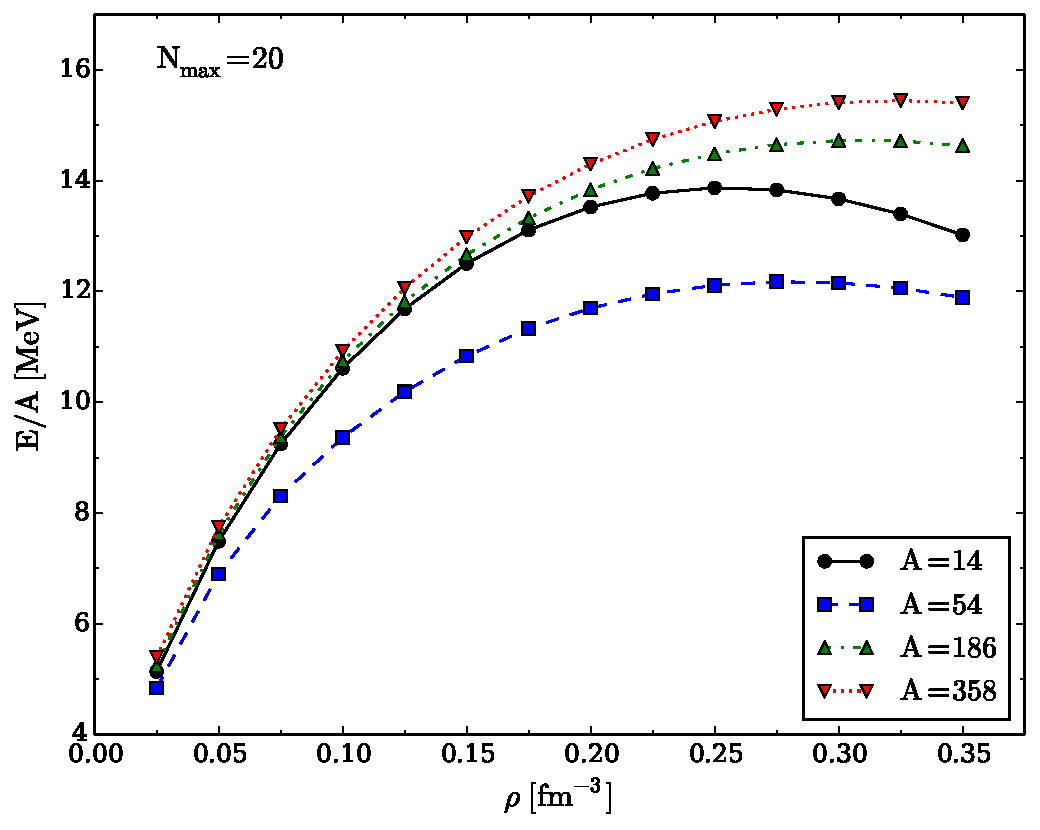
\includegraphics[width=\linewidth]{Chapter8-figures/fig1.pdf}
  \caption{Energy per particle of pure neutron matter computed in the CCD approximation with the Minnesota potential for different numbers of particles with $\mathrm{N_{max}=20}$.}
  \label{fig:fig1}
\end{figure}

\begin{figure}
  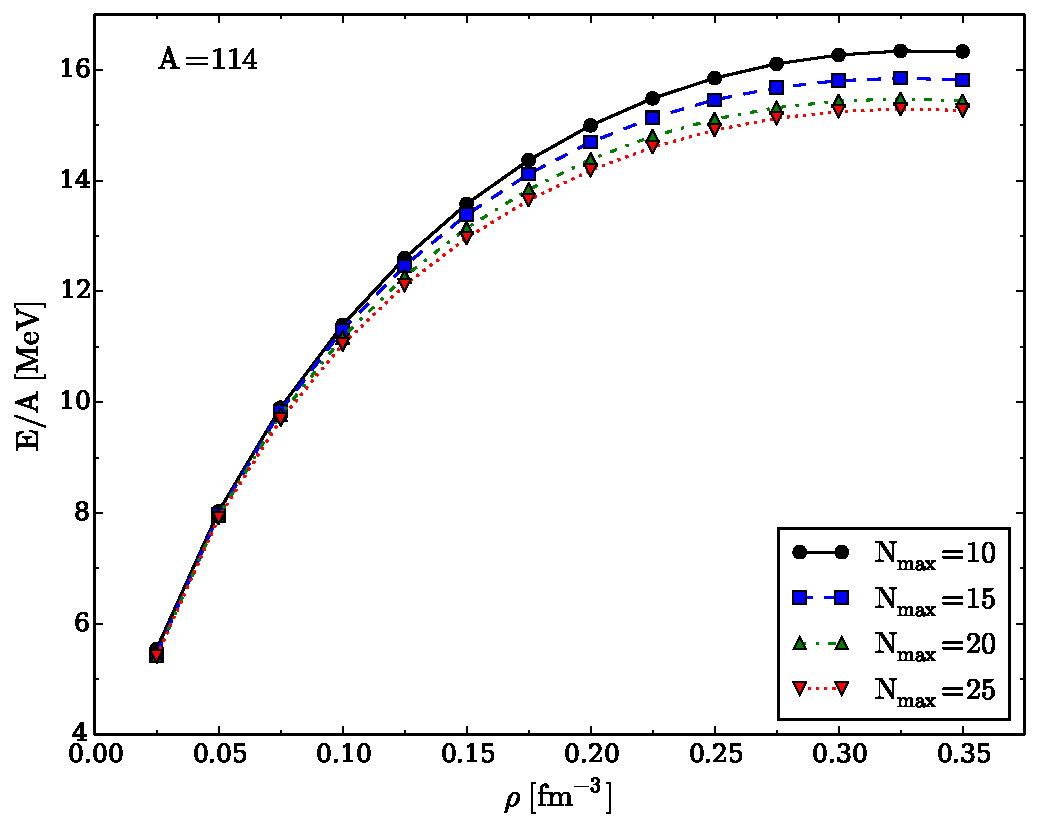
\includegraphics[width=\linewidth]{Chapter8-figures/fig2.pdf}
  \caption{Energy per particle of pure neutron matter computed in the CCD approximation with the Minnesota potential for different model space sizes with $\mathrm{A=20}$.}
  \label{fig:fig2}
\end{figure}

We approximated our problem with periodic boundary conditions, $\mathop{\phi(x_{i})}=\mathop{\phi(x_{i}+L)}$, but we could have chosen anti-periodic boundary conditions, $\mathop{\phi(x_{i})}=-\mathop{\phi(x_{i}+L)}$. The difference between these two shows how the correlation energy contains finite-size effects. One solution to this problem is by integrating over solutions between periodic and anti-periodic conditions, known as twist-averaging. First, we multiply the single-particle states by a phase for each direction, characterized by a twist-angle, $\theta_{i}$.
\begin{equation}
  \mathop{\phi_{\vec{k}}(\vec{x}+\vec{L})}\rightarrow\mathop{e^{i\vec{\theta}}\phi_{\vec{k}}(\vec{x})}
\end{equation}
$\theta_{i}=0$ for PBC and $\theta_{i}=\pi$ for APBC
\begin{align}
\vec{k}\rightarrow\vec{k}+\frac{\vec{\theta}}{L} \\
\epsilon_{\vec{k}}\rightarrow\epsilon_{\vec{k}}+\frac{\pi}{L}\vec{k}\cdot\vec{\theta}+\frac{\pi^{2}}{L^{2}}
\end{align}
Adding these phases changes the single-particle energies, the correction of which disappear as $L\rightarrow\infty$, depending on $\vec{\theta}$ and thus changes the shell structure so that hole states can jump up to particle states and vis a versa. So it's necessary to fill hole states separately for each $\vec{\theta}$. Integration over some quantitiy is approximated by a weighted sum, such as Gauss-Legendre quadrature, over the quantity for each set of twist angles.

\begin{algorithmic}
  \State Build mesh points and weights for each direction $i$: $\{\theta_{i},w_{i}\}$
  \State $E_{\text{twist}}=0$
  \For{$\mathop{(\theta_{x},w_{x})}\in\mathop{\{\theta_{x},w_{x}\}}$}
  \For{$\mathop{(\theta_{y},w_{y})}\in\mathop{\{\theta_{y},w_{y}\}}$}
  \For{$\mathop{(\theta_{z},w_{z})}\in\mathop{\{\theta_{z},w_{z}\}}$}
  \State Build Basis States with $k_{i}\rightarrow k_{i}+\frac{\theta_{i}}{L}$
  \State Order States by Energy and Fill Holes
  \State Get Result $E$ (T,HF,CCD)
  \State $E_{\text{twist}}=E_{\text{twist}}+\frac{1}{\pi^{3}}w_{x}w_{y}w_{z}E$
  \EndFor
  \EndFor
  \EndFor
\end{algorithmic}

This technique gives results which depend much less on the particle number, but requires a full calculation for each set of twist angles, which can grow very quickly. For example, using 10 twist angles in each direction requires 1000 calculations. To see the effects of twist averaging, it's easy to calculate the kinetic energy per particle and the Hartree-Fock energy per particle, which avoids the full CCD calculation. These calculations can be compared to the exact values for infinite matter, which are calculated by integrating the the relevent values up to the fermi surface.

\begin{align}
  \text{T}_{\text{inf}}=\frac{3\hbar^{2}k_{f}^{2}}{10m} \\
  \text{HF}_{\text{inf}}=\frac{1}{\mathop{(2\pi)^{6}}}\frac{L^{3}}{2\rho}\int_{0}^{k_{f}}d\vec{k}_{1}\int_{0}^{k_{f}}d\vec{k}_{2}\braket{\vec{k}_{1}\vec{k}_{2}|\hat{v}|\vec{k}_{1}\vec{k}_{2}}
\end{align}

\begin{figure}
  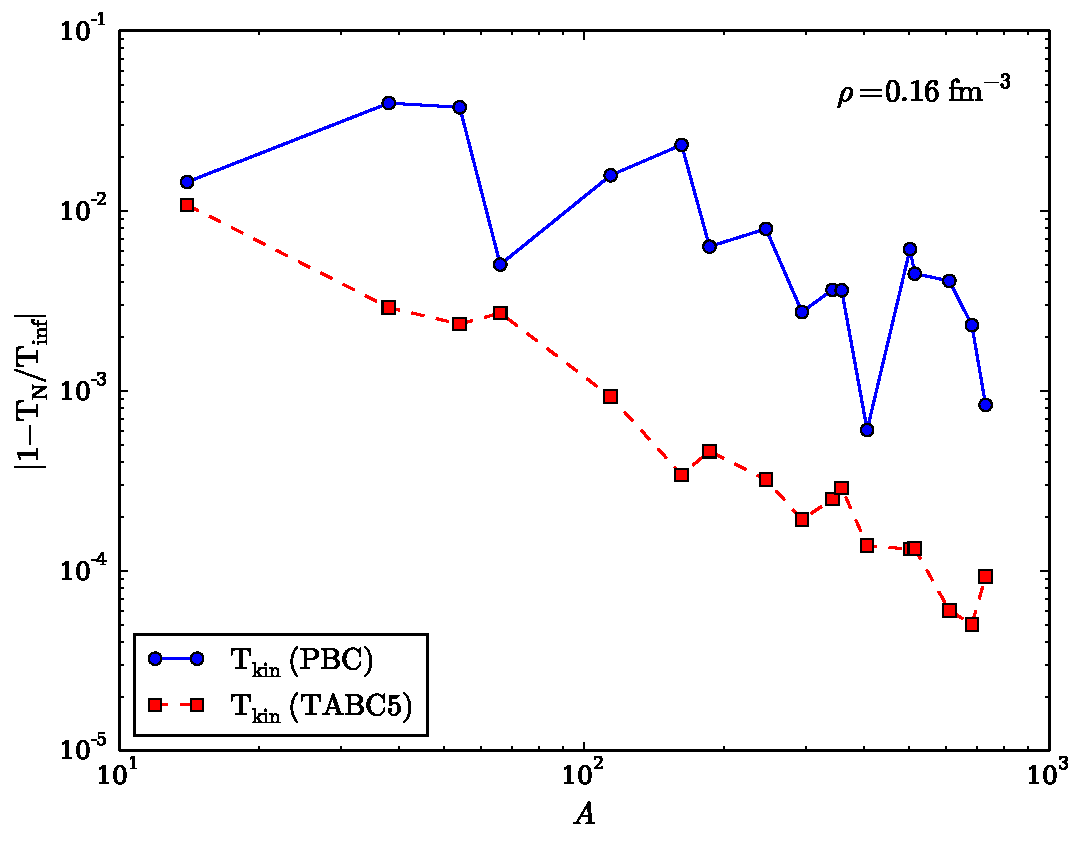
\includegraphics[width=\linewidth]{Chapter8-figures/fig3.pdf}
  \caption{Finite-size effects in the kinetic energy of pure neutron matter computed with the Minnesota potential as a function of the number of particles for both periodic boundary conditions and twist-averaged boundary conditions.}
  \label{fig:fig3}
\end{figure}

\begin{figure}
  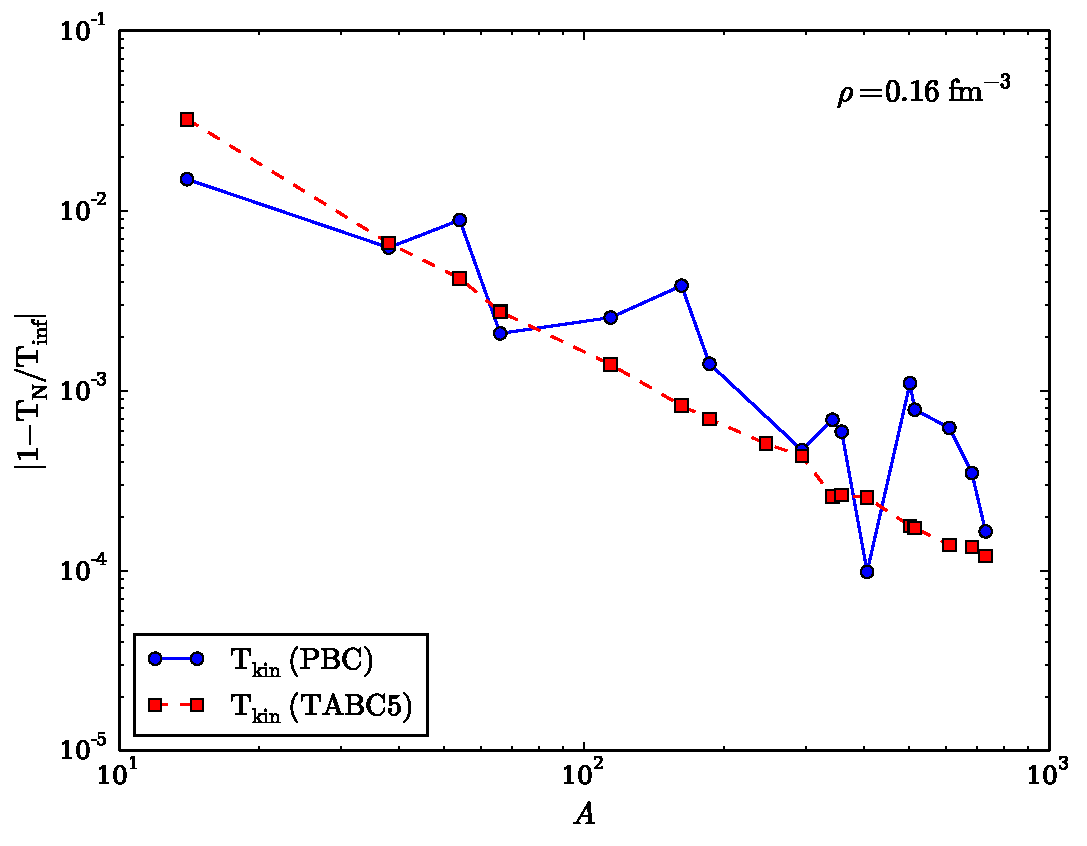
\includegraphics[width=\linewidth]{Chapter8-figures/fig4.pdf}
  \caption{Finite-size effects in the Hartree-Fock energy of pure neutron matter computed with the Minnesota potential as a function of the number of particles for both periodic boundary conditions and twist-averaged boundary conditions.}
  \label{fig:fig4}
\end{figure}


\section{Conclusions}


\section{Exercises}
\begin{prob} \label{problem:prob8.1}
Show that the one-body part of the Hamiltonian
    \begin{equation*}
        \hat{H}_0 = \sum_{pq} \element{p}{\hat{h}_0}{q} a^\dagger_p a_q
    \end{equation*}
can be written, using standard annihilation and creation operators, in normal-ordered form as 
    \begin{align*}
        \hat{H}_0 &= \sum_{pq} \element{p}{\hat{h}_0}{q} a^\dagger_p a_q \nonumber \\
            &= \sum_{pq} \element{p}{\hat{h}_0}{q} \left\{a^\dagger_p a_q\right\} + 
                \delta_{pq\in i} \sum_{pq} \element{p}{\hat{h}_0}{q} \nonumber \\
            &= \sum_{pq} \element{p}{\hat{h}_0}{q} \left\{a^\dagger_p a_q\right\} +
                \sum_i \element{i}{\hat{h}_0}{i}
    \end{align*}
Explain the meaning of the various symbols. Which reference 
vacuum has been used?
\end{prob}

\begin{sol}{problem:prob8.1}

\end{sol}

\begin{prob} \label{problem:prob8.2}
Show that the two-body part of the Hamiltonian
    \begin{equation*}
        \hat{H}_I = \frac{1}{4} \sum_{pqrs} \element{pq}{\hat{v}}{rs} a^\dagger_p a^\dagger_q a_s  a_r
    \end{equation*}
can be written, using standard annihilation and creation operators, in normal-ordered form as 
    \begin{align*}
    \hat{H}_I &= \frac{1}{4} \sum_{pqrs} \element{pq}{\hat{v}}{rs} a^\dagger_p a^\dagger_q a_s  a_r \nonumber \\
        &= \frac{1}{4} \sum_{pqrs} \element{pq}{\hat{v}}{rs} \normord{a^\dagger_p a^\dagger_q a_s  a_r}
            + \sum_{pqi} \element{pi}{\hat{v}}{qi} \normord{a^\dagger_p a_q} 
            + \frac{1}{2} \sum_{ij} \element{ij}{\hat{v}}{ij}
    \end{align*}
Explain again the meaning of the various symbols.
\end{prob}

\begin{sol}{problem:prob8.2}

\end{sol}



\begin{prob}\label{problem:prob8.3}
     Derive the normal-ordered form of the threebody part of the Hamiltonian.
    \begin{align*}
    \hat{H}_3 &= \frac{1}{36} \sum_{\substack{
                        pqr \\
                        stu}}
                 \element{pqr}{\hat{v}_3}{stu} a^\dagger_p a^\dagger_q a^\dagger_r a_u a_t a_s\\
    \end{align*}
and specify the contributions to the two-body, one-body and the scalar part.
\end{prob}

\begin{sol}{problem:prob8.3}

\end{sol}

\begin{prob}\label{problem:spbasissetup}
Develop a program which sets up a single-particle basis
for nuclear matter calculations with input a given number of nucleons and a user specificied 
density or Fermi momentum. Follow the setup discussed in Table \ref{tab:table1}. 
You need to define the number of particles $A$
and the density of the system using 
\[
\rho = g \frac{k_F^3}{6\pi^2},
\]
or by defining the Fermi momentum $k_F$.
With the density/Fermi momentum  defined and a fixed number of nucleons $A$,
we can define the length $L$ of the box used with periodic
boundary contributions via the relation
\[
  V= L^3= \frac{A}{\rho}.
\]
We can then  can use $L$ to define the spacing between
various $k$-values, that is
\[
  \Delta k = \frac{2\pi}{L}.
\]
\end{prob}
\begin{sol}{problem:spbasissetup}
The following python code sets up the quantum numbers for both infinite nuclear matter and neutron 
matter emeploying a cutoff in the value of $n$.
\begin{lstlisting}
from numpy import *

nmax =2
nshell = 3*nmax*nmax
count = 1
tzmin = 1

print "Symmetric nuclear matter:"  
print "a, nx,   ny,   nz,   sz,   tz,   nx^2 + ny^2 + nz^2"
for n in range(nshell): 
    for nx in range(-nmax,nmax+1):
         for ny in range(-nmax,nmax+1):
            for nz in range(-nmax, nmax+1):  
                for sz in range(-1,1+1):
                    tz = 1
                    for tz in range(-tzmin,tzmin+1):
                        e = nx*nx + ny*ny + nz*nz
                        if e == n:
                            if sz != 0: 
                                if tz != 0: 
                                    print count, "  ",nx,"  ",ny, "  ",nz,"  ",sz,"  ",tz,"         ",e
                                    count += 1
                                    
                                    
nmax =1
nshell = 3*nmax*nmax
count = 1
tzmin = 1
print "------------------------------------"
print "Neutron matter:"                                    
print "a, nx,   ny,   nz,   sz,    nx^2 + ny^2 + nz^2"
for n in range(nshell): 
    for nx in range(-nmax,nmax+1):
         for ny in range(-nmax,nmax+1):
            for nz in range(-nmax, nmax+1):  
                for sz in range(-1,1+1):
                    e = nx*nx + ny*ny + nz*nz
                    if e == n:
                        if sz != 0: 
                            print count, "  ",nx,"  ",ny, "  ",sz,"  ",tz,"         ",e
                            count += 1                  
\end{lstlisting}                               
\end{sol}


\begin{problem}\label{problem:fourier}
The interaction we will use for these calculations is a semirealistic nucleon-nucleon potential known as the Minnesota potential \cite{minnesota} which has the form, $V_{\alpha}\left( r\right)=V_{\alpha}\exp{-(\alpha r^{2})}$. The spin and isospin dependence of the Minnesota potential is given by,
\[
V\left( r\right)=\frac{1}{2}\left( V_{R}+\frac{1}{2}\left( 1+P_{12}^{\sigma}\right) V_{T}+\frac{1}{2}\left( 1-P_{12}^{\sigma}\right) V_{S}\right)\left( 1-P_{12}^{\sigma}P_{12}^{\tau}\right),
\]
where $P_{12}^{\sigma}=\frac{1}{2}\left( 1+\sigma_{1}\cdot\sigma_{2}\right)$ and $P_{12}^{\tau}=\frac{1}{2}\left( 1+\tau_{1}\cdot\tau_{2}\right)$ are the spin and isospin exchange operators, respectively. 
Show that a Fourier transform to momentum space results in 
\[
\langle \mathbf{k}_p \mathbf{k}_q \vert V_{\alpha}\vert \mathbf{k}_r\mathbf{k}_s\rangle=\frac{V_{\alpha}}{L^{3}}\left(\frac{\pi}{\alpha}\right)^{3/2}\exp{\frac{-q^{2}}{4\alpha}}\delta_{\vec{k}_{p}+\vec{k}_{q},\vec{k}_{r}+\vec{k}_{s}}.
\]
Write thereafter a function which sets up the full anty-symmetrized matrix elements for the Minnesota potential using the parameters 
listed in Table \ref{tab:minnesotatab}. 
\end{problem}



\begin{prob}
Consider a Slater determinant built up of orthogonal single-particle orbitals $\psi_{\lambda}$, 
with $\lambda = 1,2,\dots,A$.

The unitary transformation
\[
\psi_a  = \sum_{\lambda} C_{a\lambda}\phi_{\lambda},
\]
brings us into the new basis.  
The new basis has quantum numbers $a=1,2,\dots,A$.
Show that the new basis is orthogonal.
\begin{enumerate}
\item[a)] Show that the new Slater determinant constructed from the new single-particle wave functions can be
written as the determinant based on the previous basis and the determinant of the matrix $C$.
\item[b)]
Show that the old and the new Slater determinants are equal up to a complex constant with absolute value unity.
Hint: $C$ is a unitary matrix. 
\end{enumerate}
\end{prob}


\begin{prob}
We will assume that we can build various Slater determinants using an orthogonal  single-particle basis $\psi_{\lambda}$, 
with $\lambda = 1,2,\dots,A$. 


The aim of this exercise is to set up specific matrix elements that will turn useful when we start our discussions of the nuclear shell model. In particular you will notice, depending on the character of the operator, that many matrix elements will actually be zero.

Consider three $A$-particle  Slater determinants  $|\Phi_0$, $|\Phi_i^a\rangle$ and $|\Phi_{ij}^{ab}\rangle$, where the notation means that 
Slater determinant $|\Phi_i^a\rangle$ differs from $|\Phi_0\rangle$ by one single-particle state, that is a single-particle
state $\psi_i$ is replaced by a single-particle state $\psi_a$. 
It will later be interpreted as a so-called one-particle-one-hole excitation.
Similarly, the Slater determinant $|\Phi_{ij}^{ab}\rangle$
differs by two single-particle states from $|\Phi_0\rangle$ and is normally thought of as a two-particle-two-hole excitation.

Define a general one-body operator $\hat{F} = \sum_{i}^A\hat{f}(x_{i})$ and a general  two-body operator $\hat{G}=\sum_{i>j}^A\hat{g}(x_{i},x_{j})$ with $g$ being invariant under the interchange of the coordinates of particles $i$ and $j$. 
\begin{enumerate}
\item[a)]
\[
\langle \Phi_0 \vert\hat{F}\vert\Phi_0\rangle,
\]
and
\[
\langle \Phi_0\vert\hat{G}|\Phi_0\rangle.
\]
\item[b)]
Find thereafter 
\[
\langle \Phi_0 |\hat{F}|\Phi_i^a\rangle,
\]
and
\[
\langle \Phi_0|\hat{G}|\Phi_i^a\rangle,
\]
\item[c)]
Finally, find
\[
\langle \Phi_0 |\hat{F}|\Phi_{ij}^{ab}\rangle,
\]
and
\[
\langle \Phi_0|\hat{G}|\Phi_{ij}^{ab}\rangle.
\]
\item[d)]
What happens with the two-body operator if we have a transition probability  of the type
\[
\langle \Phi_0|\hat{G}|\Phi_{ijk}^{abc}\rangle,
\]
where the Slater determinant to the right of the operator differs by more than two single-particle states?
\item[e)]
With an orthogonal basis of Slater determinants $\Phi_{\lambda}$, we can now construct an exact many-body state as a linear expansion of Slater determinants, that is, a given exact state
\[
\Psi_i = \sum_{\lambda =0}^{\infty}C_{i\lambda}\Phi_{\lambda}.
\]
In all practical calculations the infinity is replaced by a given truncation in the sum. 

If you are to compute the expectation value of (at most) a two-body Hamiltonian for the above
exact state
\[
\langle \Psi_i \vert \hat{H} \vert \Psi_i\rangle,
\]
based on the calculations above, which are the only elements which will contribute?  (there is no need to perform any calculation here, use your results from exercises a), b), and c)).

These results simplify to a large extent shell-model calculations. 
\end{enumerate}
\end{prob}



\begin{prob}\label{problem:prob8.4}


We present a simplified Hamiltonian consisting of an unperturbed
Hamiltonian and a so-called pairing interaction term. It is a model
which to a large extent mimicks some central features of atomic
nuclei, certain atoms and systems which exhibit superfluiditity or
superconductivity.  To study this system, we will use a mix of
many-body perturbation theory (MBPT), Hartree-Fock (HF) theory and full
configuration interaction (FCI) theory. The latter will also provide us with
the exact answer.  When setting up the Hamiltonian matrix you will
need to solve an eigenvalue problem.

We define first the Hamiltonian, with a definition of the model space
and the single-particle basis. Thereafter, we present the various
exercises (some of them are solved).


The Hamiltonian acting in the complete Hilbert space (usually infinite
dimensional) consists of an unperturbed one-body part, $\hat{H}_0$,
and a perturbation $\hat{V}$.

We limit ourselves to at most two-body interactions and our Hamiltonian
is represented by the following operators
\[
\hat{H} = \sum_{\alpha\beta}\langle \alpha |h_0|\beta\rangle
a_{\alpha}^{\dagger}a_{\beta}+\frac{1}{4}\sum_{\alpha\beta\gamma\delta}\langle \alpha\beta|
V|\gamma\delta\rangle a_{\alpha}^{\dagger}a_{\beta}^{\dagger}a_{\delta}a_{\gamma},
\]
where $a_{\alpha}^{\dagger}$ and $a_{\alpha}$ etc.~are standard
fermion creation and annihilation operators, respectively, and
$\alpha\beta\gamma\delta$ represent all possible single-particle
quantum numbers.  The full single-particle space is defined by the
completeness relation
\[
\hat{{\bf 1}} = \sum_{\alpha=1}^{\infty}|\alpha \rangle \langle \alpha|.
\]
In our calculations
we will let the single-particle states $|\alpha\rangle$ be
eigenfunctions of the one-particle operator $\hat{h}_0$. Note that the two-body part of the Hamiltonian
contains anti-symmetrized matrix elements.


The above Hamiltonian acts in turn on various many-body Slater
determinants constructed from the single-basis defined by the one-body
operator $\hat{h}_0$.  As an example, the two-particle model space
$\mathcal{P}$ is defined by an operator
\[
\hat{P} = \sum_{\alpha\beta =1}^{m}|\alpha\beta \rangle \langle
\alpha\beta|,
\]
where we assume that $m=\dim(\mathcal{P})$ and the full space is
defined by
\[
\hat{P}+\hat{Q}=\hat{{\bf 1}},
\]
with the projection operator
\[
\hat{Q} = \sum_{\alpha\beta =m+1}^{\infty}|\alpha\beta \rangle \langle
\alpha\beta|,
\]
being the complement of $\hat{P}$.


Our specific model consists of $N$ doubly-degenerate and equally
spaced single-particle levels labelled by $p=1,2,\dots$ and spin
$\sigma=\pm 1$.  These states are schematically portrayed in
Fig.~\ref{fig:schematic}.  The first two single-particle levels define
a possible model space, indicated by the label $\mathcal{P}$.  The
remaining states span the excluded space $\mathcal{Q}$.

We write the Hamiltonian as
\[ \hat{H} = \hat{H}_0 + \hat{V} , \]
where
\[
\hat{H}_0=\xi\sum_{p\sigma}(p-1)a_{p\sigma}^{\dagger}a_{p\sigma}
\]
and
\[
\hat{V}=-\frac{1}{2}g\sum_{pq}a^{\dagger}_{p+}
a^{\dagger}_{p-}a_{q-}a_{q+}.
\]
Here, $H_0$ is the unperturbed Hamiltonian with a spacing between
successive single-particle states given by $\xi$, which we will set to
a constant value $\xi=1$ without loss of generality. The two-body
operator $\hat{V}$ has one term only. It represents the pairing
contribution and carries a constant strength $g$.

The indices
$\sigma=\pm$ represent the two possible spin values. The interaction
can only couple pairs and excites therefore only two particles at the
time.


\begin{enumerate}
\item[a)]
Show that the unperturbed Hamiltonian $\hat{H}_0$ and $\hat{V}$
  commute with both the spin projection $\hat{S}_z$ and the total spin
  $\hat{S}^2$, given by
\[
  \hat{S}_z := \frac{1}{2}\sum_{p\sigma} \sigma
  a^{\dagger}_{p\sigma}a_{p\sigma}
\]
and
\[
  \hat{S}^2 := \hat{S}_z^2 + \frac{1}{2}(\hat{S}_+\hat{S}_- +
  \hat{S}_-\hat{S}_+),
\]
where
\[
  \hat{S}_\pm := \sum_{p} a^{\dagger}_{p\pm} a_{p\mp}.
\]
This is an important feature of our system that allows us to
block-diagonalize the full Hamiltonian. We will focus on total spin
$S=0$.  In this case, it is convenient to define the so-called pair
creation and pair annihilation operators
\[
\hat{P}^{+}_p = a^{\dagger}_{p+}a^{\dagger}_{p-},
\]
and
\[
\hat{P}^{-}_p = a_{p-}a_{p+},
\]
respectively.
\item[b)]
Show that you can rewrite the Hamiltonian (with $\xi=1$) as
\[
\hat{H}=\sum_{p\sigma}(p-1)a_{p\sigma}^{\dagger}a_{p\sigma}
-\frac{1}{2}g\sum_{pq}\hat{P}^{+}_p\hat{P}^{-}_q.
\]
\item[c)]
Show also that Hamiltonian commutes with the product of the pair
creation and annihilation operators.  This model corresponds to a
system with no broken pairs. This means that the Hamiltonian can only
link two-particle states in so-called spin-reversed states.

\item[d)]
Construct thereafter the Hamiltonian matrix for a system with no
  broken pairs and total spin $S=0$ for the case of the four lowest
  single-particle levels indicated in the
  Fig.~\ref{fig:schematic}. Our system consists of four particles
  only.  Our single-particle space consists of only the four lowest
  levels $p=1,2,3,4$.  You need to set up all possible Slater
  determinants.  Find all eigenvalues by diagonalizing the Hamiltonian
  matrix.  Vary your results for values of $g\in [-1,1]$.  We refer to
  this as the exact calculation. Comment the behavior of the ground
  state as function of $g$.
\end{enumerate}
\end{prob}

\begin{sol}{problem:prob8.4}
We give first the final Hamiltonian matrix
!bt
\[
H = \left (
\begin{array}{cccccc}
2\delta -g & -g/2 & -g/2 & -g/2 & -g/2 & 0 \\
 -g/2 & 4\delta -g & -g/2 & -g/2 & -0 & -g/2 \\
-g/2 & -g/2 & 6\delta -g & 0 & -g/2 & -g/2 \\
 -g/2 & -g/2 & 0 & 6\delta-g & -g/2 & -g/2 \\
 -g/2 & 0 & -g/2 & -g/2 & 8\delta-g & -g/2 \\
0 & -g/2 & -g/2 & -g/2 & -g/2 & 10\delta -g
\end{array} \right )
\]

The following python program diagonalizes the above Hamiltonian matrix for a given span of interaction strength values, performing both a full configuration interaction calculation and a truncated one. For the truncated case we leave out the $4p4h$ state. This means that in addition to the ground state we include the four possible $2p2h$ states. Such a calculation is normally called a configuration interaction calculation.
\begin{lstlisting}
from numpy import *
from sympy import *
from matplotlib.pyplot import *

g_array = linspace(-1, 1, 1001)
e1_array = []
e2_array = []

for g in g_array:
	H1 = matrix([[2-g , -g/2.,  -g/2., -g/2., -g/2.,     0],
		        [-g/2.,   4-g,  -g/2., -g/2.,    0., -g/2.],
		        [-g/2., -g/2.,    6-g,     0, -g/2., -g/2.],
				[-g/2., -g/2.,      0,   6-g, -g/2., -g/2.],
				[-g/2.,     0,  -g/2., -g/2.,   8-g, -g/2.],
				[0    , -g/2.,  -g/2., -g/2., -g/2.,  10-g]])

	H2 = matrix([[2-g , -g/2.,  -g/2., -g/2., -g/2.],
		        [-g/2.,   4-g,  -g/2., -g/2.,    0.],
		        [-g/2., -g/2.,    6-g,     0, -g/2.],
				[-g/2., -g/2.,      0,   6-g, -g/2.],
				[-g/2.,     0,  -g/2., -g/2.,   8-g]])



	u1, v1 = linalg.eig(H1)
	u2, v2 = linalg.eig(H2)

	if g == 1./2:
		print argmin(u1)

		for i in range(5):
			print " %.3f " % v2[i,0],



	e1_array.append(min(u1))
	e2_array.append(min(u2))


plot(g_array, e1_array, linewidth=2.0)
#plot(g_array, e2_array, linewidth=2.0)
plot(g_array, (2-g_array), linewidth=2.0)
grid()
xlabel(r"Strength of interaction, $g$", fontsize=16)
ylabel(r'Ground state energy', fontsize=16)
#axis([-1,1,-0.4,0.05])
legend(['FCI -- Exact', 'Reference energy'])
savefig("pairing.pdf")
show()
\end{lstlisting}
The eigenvalues and eigenvectors result from the diagonalization of the above Hamiltonian matrix.
In the discussions below and in connection with the first stage of the numerical project, we will use these results to benchmark various approximative methods.
The lowest eigenvalue corresponds to the ground state
energy and we will refer to it as the *exact energy* when no truncations in the space of possible Slater determinants are made..

From our results, we note some important differences between the full configuration interaction (FCI)
calculation and the truncated configuration interaction calculation (CI).
Full configuration interaction is an exact method, but is only
possible if and only if we have a complete and finite SD basis for our
system. In practice, we usually don't have this. Non-complete
CI however, is always possible, but yiels   approximative
results only. The method is however still variational however, meaning that we
guaranteed that the approximation will be equal or bigger to the true
result.
Perturbation theory however, is non-variational and there is no guarantee that including higher orders in the
perturbation gives an improved result, as we will see below.

In an FCI case, we are including all possible exictations to infinite
order, meaning we have all possible $1p1h$ , $2p2h$ etc configurations, up to $4p4h$
excitations for our selected model. Due to the nature of the pairing interaction and our selection
of specific quantum numbers for the many-body states, we do not have any $1p1h$ or $3p3h$ excitations.
In the above CI case, we truncate those excitations somewhere.
If we
were to draw the diagrams of the interactions that contribute to this
CI case, there would be an infinite number of them, as we can have
arbitrarily long chains of operators that still only have at most 2p2h
intermediate states.
\end{sol}


\begin{prob}\label{problem:prob8.4}
\begin{enumerate}
\item[a)]
We will now set up the Hartree-Fock equations by varying the
coefficients of the single-particle functions. The single-particle
basis functions are defined as
\[
\psi_p = \sum_{\lambda} C_{p\lambda}\psi_{\lambda}.
\]
where in our case $p=1,2,3,4$ and $\lambda=1,2,3,4$, that is the first
four lowest single-particle orbits of Fig.~\ref{fig:schematic}.  Set
up the Hartree-Fock equations for this system by varying the
coefficients $C_{p\lambda}$ and solve them for values of $g\in
[-1,1]$.  Comment your results and compare with the exact
solution. Discuss also which diagrams in Fig.~\ref{fig:diagrams} that
can be affected by a Hartree-Fock basis. Compute the total binding
energy using a Hartree-Fock basis and comment your results.

\item[b)]
We will now study the system using non-degenerate
Rayleigh-Schroedinger perturbation theory to third order in the
interaction.  If we exclude the first order contribution, all possible
diagrams (so-called anti-symmetric Goldstone diagrams) are
shown in Fig.~\ref{fig:diagrams}.


Based on the form of the interaction, which diagrams contribute to the
binding energy of the ground state?  Write down the expressions for
the diagrams that contribute and find the contribution to the ground
state energy as function $g\in [-1,1]$. Comment your results.  Compare
these results with those you obtained from the exact diagonalization with and without the $4p-4h$ state.
Discuss your results for a canonical Hartree-Fock basis and a non-canonical Hartree-Fock basis.


Diagram 1 in Fig.~\ref{fig:diagrams} represents a second-order contribution to the energy and a so-called $2p-2h$ contribution to the intermediate states. Write down the expression for the wave operator in this case and compare the possible contributions with the configuration interaction calculations without the $4p-4h$ Slater determinant. Comment your results for
various values of $g\in [-1,1]$.

We limit now the discussion to the canonical Hartree-Fock case only. To fourth order in perturbation theory we can produce diagrams with $1p-1h$ intermediate excitations as shown in Fig.~\ref{fig:fourthorder1p1h}, $2p-2h$ excitations, see Fig.~\ref{fig:fourthorder2p2h}, $3p-3h$ excitations as shown in Fig.~\ref{fig:fourthorder3p3h} and finally so-called diagrams with intermediate four-particle-four-hole excitations, see Fig.~\ref{fig:fourthorder4p4h}.

Define first linked and unlinked diagrams and explain briefly Goldstone's linked diagram theorem.
Based on the linked diagram theorem and the form of the pairing Hamiltonian, which diagrams will contribute
to fourth order?

Calculate the energy to fourth order with a canonical Hartree-Fock basis for $g\in [-1,1]$ and compare
with the full diagonalization case in exercise b). Discuss the results.
\end{enumerate}


To fourth order in the interaction there are several diagrams to consider.
Fortunately, due to the character of the pairing Hamiltonian, several of these contributions are
zero. We limit our discussions also to include the
canonical HF-case only.
All of the diagrams in the canonical case are
shown in figures 3, 4, 5 and 6 above.
Using also the linked diagram theorem, where a
diagram is called unlinked if and only if it has a disconnected part
that is closed, we can eliminate some further  diagrams. Goldstones
linked-diagram theorem states that all unliked diagrams will cancel
against the renormalization terms in Rayleigh-Schroedinger perturbation theory,
meaning that we can define
the energy to each order as a sum of linked diagrams
only. We can then disregard diagram 33 and 41.

Let us now go through all the diagrams and find those that vanish due
to having broken pairs, i.e., the diagrams that vanish due to our
specific interaction. Take for example diagram 1, which vanishes due
to having a term $\langle ab\vert \hat{v} \vert ci\rangle$. From this
argument, we see that all four diagrams from figure 3 vanish. Similar
arguments shows that most diagrams in figure 4 also dissapear. Going
through all the diagrams, we see that 5, 6, 14 and 15 are the ones
that do not vanish in figure 4. For figure 5 we actually see that all
diagrams vanish again. For figure 6 we already found that 33 and 41
vanished due to being unlinked---the rest contribute to the perturbative expansion of the
energy.
The diagrams of figures 3 and 5 vanish since they involve $1p1h$ and $3p3h$ excitations, respectively.

The expressions for these diagrams can easily be written in terms of a
simple Python program. Note however that for every diagram we do
actually perform loops over every single-particle state. As we will
see later, this is extremely inefficient from a computational point
of view. In our discussions of the projects below, we will rewrite the
computations of most diagrams in terms of efficient matrix-matrix
multiplications or matrix-vector multiplications.  The following
Python program gives us the final results for perturbation theory to fourth
order in the interaction. The resulting figures include also plots of the relative error in the
correlation energy. That is, we compare the computed correlation in
perturbation theory with the result from the exact diagonalization discussed above.

\begin{lstlisting}
from sympy import *
from pylab import *

below_fermi = (0,1,2,3)
above_fermi = (4,5,6,7)

states = [(1,1),(1,-1),(2,1),(2,-1),(3,1),(3,-1),(4,1),(4,-1)]
N = 8
g = Symbol('g')



def h0(p,q):
	if p == q:
		p1, s1 = states[p]
		return (p1 - 1)
	else:
		return 0

def f(p,q):
	if p == q:
		return 0

	s = h0(p,q)
	for i in below_fermi:
		s += assym(p,i,q,i)
	return s


def assym(p,q,r,s):
	p1, s1 = states[p]
	p2, s2 = states[q]
	p3, s3 = states[r]
	p4, s4 = states[s]

	if p1 != p2 or p3 != p4:
		return 0
	if s1 == s2 or s3 == s4:
		return 0
	if s1 == s3 and s2 == s4:
		return -g/2.
	if s1 == s4 and s2 == s3:
		return g/2.

def eps(holes, particles):
	E = 0
	for h in holes:
		p, s = states[h]
		E += (p-1)
	for p in particles:
		p, s = states[p]
		E -= (p-1)
	return E


# Diagram 3
# s = 0
# for a in above_fermi:
# 	for b in above_fermi:
# 		for c in above_fermi:
# 			for i in below_fermi:
# 				for j in below_fermi:
# 					for k in below_fermi:
# 						s += assym(i,j,a,b)*assym(a,c,j,k)*assym(b,k,c,i)/eps((i,j),(a,b))/eps((k,j),(a,c))
# print s


# ga = linspace(-1,1,101)
# corr2 = []
# corr3 = []
# corrx = []


# Diagram 1
s1 = 0
for a in above_fermi:
	for b in above_fermi:
		for i in below_fermi:
			for j in below_fermi:
				s1 += 0.25*assym(a,b,i,j)*assym(i,j,a,b)/eps((i,j),(a,b))

# Diagram 4
s4 = 0
for a in above_fermi:
	for b in above_fermi:
		for c in above_fermi:
			for d in above_fermi:
				for i in below_fermi:
					for j in below_fermi:
						s4 += 0.125*assym(i,j,a,b)*assym(a,b,c,d)*assym(c,d,i,j)/eps((i,j),(a,b))/eps((i,j),(c,d))

# Diagram 5
s5 = 0
for a in above_fermi:
	for b in above_fermi:
		for i in below_fermi:
			for j in below_fermi:
				for k in below_fermi:
					for l in below_fermi:
						s5 += 0.125*assym(i,j,a,b)*assym(k,l,i,j)*assym(a,b,k,l)/eps((i,j),(a,b))/eps((k,l),(a,b))

# Diagram 8 (simplified)
s8 = 0
for a in above_fermi:
	for b in above_fermi:
		for i in below_fermi:
			for j in below_fermi:
				for k in below_fermi:
					s8 -= 0.5*assym(i,j,a,b)*assym(a,b,i,k)*f(k,j)/eps((i,j),(a,b))/eps((i,k),(a,b))

# Diagram 9 (simplified)
s9 = 0
for a in above_fermi:
	for b in above_fermi:
		for c in above_fermi:
			for i in below_fermi:
				for j in below_fermi:
					s9 += 0.5*assym(i,j,a,b)*assym(a,c,i,j)*f(b,c)/eps((i,j),(a,b))/eps((i,j),(a,c))


print s1
print s4
print s5
print s8
print s9

s_5 =  -0.0291521990740741*g**4
s14 =  -0.0308883101851853*g**4
s34 =  0.0163049768518519*g**4
s36 =  -0.0145760995370371*g**4
s38 =  -0.0201099537037037*g**4
s39 =  0.0176938657407407*g**4

ga = linspace(-1,1,10001)
e1 = []
corr2 = []
corr3 = []
corr4 = []
for g_val in ga:
	H1 = matrix([[2-g_val , -g_val/2.,  -g_val/2., -g_val/2., -g_val/2.,     0],
		        [-g_val/2.,   4-g_val,  -g_val/2., -g_val/2.,    0., -g_val/2.],
		        [-g_val/2., -g_val/2.,    6-g_val,     0, -g_val/2., -g_val/2.],
				[-g_val/2., -g_val/2.,      0,   6-g_val, -g_val/2., -g_val/2.],
				[-g_val/2.,     0,  -g_val/2., -g_val/2.,   8-g_val, -g_val/2.],
				[0    , -g_val/2.,  -g_val/2., -g_val/2., -g_val/2.,  10-g_val]])

	u1, v1 = linalg.eig(H1)
	e1.append(min(u1))

	corr2.append((s1).subs(g,g_val))
	corr3.append((s1+s4+s5).subs(g,g_val))
	corr4.append((s1+s4+s5+2*s_5+2*s14+2*s34+2*s36+s38+2*s39).subs(g,g_val))

exact = e1 - (2-ga)

plot(ga, exact, linewidth=2.0)
plot(ga, corr2, linewidth=2.0)
plot(ga, corr3, linewidth=2.0)
plot(ga, corr4, linewidth=2.0)
xlabel(r'Interaction strength, $g$', fontsize=16)
ylabel(r'Correlation energy', fontsize=16)
axis([-1,1,-0.5,0.05])
grid()
legend(["Exact", "2. order MPBT", "3. order MPBT", "4. order MPBT"], 'lower left')
savefig("perturbationtheory.pdf")
show()
error1 = zeros(len(exact))
error2 = zeros(len(exact))
error3 = zeros(len(exact))

for i in range(len(exact)):
	error1[i] = abs(float(exact[i]-corr2[i]))
	error2[i] = abs(float(exact[i]-corr3[i]))
	error3[i] = abs(float(exact[i]-corr4[i]))

error1 = array(error1)
error2 = array(error2)
error3 = array(error3)
print type(error1)

plot(ga, log10(error1))
plot(ga, log10(error2))
plot(ga, log10(error3))
xlabel(r"Strength of interaction, $g$", fontsize=16)
ylabel(r"Error, $\log_{\rm 10}({\rm abs}({\rm error})$", fontsize=16)
legend(["2. order MPBT", "3. order MPBT", "4. order MPBT"], 'lower left')
grid()
savefig("logerror.pdf")
show()
\end{lstlisting}

Running the Python program shows us that
the approximation to both second and third order are very
good when the interaction strength is small and contained in the interval
$g\in[-0.5,0.5]$, but as the
interaction gets stronger the approximation worsens. We also
note that the third-order result is actually worse than the second order result
for larger values of the interaction strength, indicating that there is no guarantee that higher orders
in many-body perturbation theory may reduce the relative error in a systematic way.
This is seen in particular for the results to fourth order. For negative interaction strengths
fourth order gives a better result than second and third order, while for $g>0$ the relative error is
worse.
We note also the non-variational character of many-body perturbation theory, with results at different undershooting the true ground state correlation energy

\end{prob}


\begin{prob}\label{problem:prob8.6}
This project serves as a continuation
of the pairing model with the aim being to solve the same problem but
now by developing a program that implements the coupled cluster method
with double excitations only. In doing so you will find it convenient
to write classes which define the single-particle basis and the
Hamiltonian. Your functions that solve the coupled cluster equations
will then just need to set up variables which point to interaction
elements and single-particle states with their pertinent quantum
numbers. Use for example the setup discussed in the FCI lectures for
the pairing model.

\begin{enumerate}

\item[a)]
Explain why no single excitations are involved in this model.


\item[b)]
Set up the coupled cluster equations for doubles excitations and convince yourself about their
meaning and correctness.

\item[c)]
Write a class which holds
single-particle data like specific quantum numbers, single-particle
Hamiltonian etc. Write also a class which sets up and stores two-body
matrix elements defined by the single-particle states.  Write
thereafter functions/classes which implement the coupled cluster
method with doubles only.


\item[d)]
Compare your results with
those from the exact diagonalization with and without the $4p4h$
excitation. Compare also your results to perturbation theory at
different orders, in particular to second order. Discuss your results.
If other students are solving the same problem using Green's function
theory, you can also compare your results with those obtained from
Green's function theory. The aim is to finalize this part during the
first week. The codes you will develop can be used as a starting point
for the second part of the project.
\end{enumerate}
\end{prob}


\begin{acknowledgement}
We are much indebted to Thomas Papenbrock for many discussions on many-body physics.
Computational resources were provided by Michigan State University and the Research Council of Norway via the Notur project (Supercomputing grant NN2977K).
This work was supported by NSF Grant No. PHY-1404159 (Michigan State University)  and  the Research Council of Norway under contract ISP-Fysikk/216699.
\end{acknowledgement}



\bibliographystyle{spphys}
\bibliography{lnplib}





 

% Slides for FYS-KJM4480


\documentclass[compress]{beamer}


% Try the class options [notes], [notes=only], [trans], [handout],
% [red], [compress], [draft], [class=article] and see what happens!

% For a green structure color use:
%\colorlet{structure}{green!50!black}

\mode<article> % only for the article version
{
  \usepackage{beamerbasearticle}
  \usepackage{fullpage}
  \usepackage{hyperref}
}

\beamertemplateshadingbackground{red!10}{blue!10}

%\beamertemplateshadingbackground{red!10}{blue!10}
\beamertemplatetransparentcovereddynamic
%\usetheme{Hannover}

\setbeamertemplate{footline}[page number]


%\usepackage{beamerthemeshadow}

%\usepackage{beamerthemeshadow}
\usepackage{ucs}


\usepackage{pgf,pgfarrows,pgfnodes,pgfautomata,pgfheaps,pgfshade}
\usepackage{graphicx}
\usepackage{simplewick}
\usepackage{amsmath,amssymb}
\usepackage[latin1]{inputenc}
\usepackage{colortbl}
\usepackage[english]{babel}
\usepackage{listings}
\usepackage{shadow}
\lstset{language=c++}
\lstset{alsolanguage=[90]Fortran}
\lstset{basicstyle=\small}
%\lstset{backgroundcolor=\color{white}}
%\lstset{frame=single}
\lstset{stringstyle=\ttfamily}
%\lstset{keywordstyle=\color{red}\bfseries}
%\lstset{commentstyle=\itshape\color{blue}}
\lstset{showspaces=false}
\lstset{showstringspaces=false}
\lstset{showtabs=false}
\lstset{breaklines}
\usepackage{times}

% Use some nice templates
\beamertemplatetransparentcovereddynamic

% own commands
\newcommand*{\cre}[1]{a^{\dagger}_{#1}}
\newcommand*{\an}[1]{a_{#1}}
\newcommand*{\crequasi}[1]{b^{\dagger}_{#1}}
\newcommand*{\anquasi}[1]{b_{#1}}
\newcommand*{\for}[3]{\langle#1|#2|#3\rangle}
\newcommand{\be}{\begin{equation}}
\newcommand{\ee}{\end{equation}}
\newcommand*{\kpr}[1]{\left\{#1\right\}}
\newcommand*{\ket}[1]{|#1\rangle}
\newcommand*{\bra}[1]{\langle#1|}
%\newcommand{\bra}[1]{\left\langle #1 \right|}
%\newcommand{\ket}[1]{\left| # \right\rangle}
\newcommand{\braket}[2]{\left\langle #1 \right| #2 \right\rangle}
\newcommand{\OP}[1]{{\bf\widehat{#1}}}
\newcommand{\matr}[1]{{\bf \cal{#1}}}
\newcommand{\beN}{\begin{equation*}}
\newcommand{\bea}{\begin{eqnarray}}
\newcommand{\beaN}{\begin{eqnarray*}}
\newcommand{\eeN}{\end{equation*}}
\newcommand{\eea}{\end{eqnarray}}
\newcommand{\eeaN}{\end{eqnarray*}}
\newcommand{\bdm}{\begin{displaymath}}
\newcommand{\edm}{\end{displaymath}}
\newcommand{\bsubeqs}{\begin{subequations}}
\newcommand*{\fpr}[1]{\left[#1\right]}
\newcommand{\esubeqs}{\end{subequations}}
\newcommand*{\pr}[1]{\left(#1\right)}
\newcommand{\element}[3]
        {\bra{#1}#2\ket{#3}}

\newcommand{\md}{\mathrm{d}}
\newcommand{\e}[1]{\times 10^{#1}}
\renewcommand{\vec}[1]{\mathbf{#1}}
\newcommand{\gvec}[1]{\boldsymbol{#1}}
\newcommand{\dr}{\, \mathrm d^3 \vec r}
\newcommand{\dk}{\, \mathrm d^3 \vec k}
\def\psii{\psi_{i}}
\def\psij{\psi_{j}}
\def\psiij{\psi_{ij}}
\def\psisq{\psi^2}
\def\psisqex{\langle \psi^2 \rangle}
\def\psiR{\psi({\bf R})}
\def\psiRk{\psi({\bf R}_k)}
\def\psiiRk{\psi_{i}(\Rveck)}
\def\psijRk{\psi_{j}(\Rveck)}
\def\psiijRk{\psi_{ij}(\Rveck)}
\def\ranglep{\rangle_{\psisq}}
\def\Hpsibypsi{{H \psi \over \psi}}
\def\Hpsiibypsi{{H \psii \over \psi}}
\def\HmEpsibypsi{{(H-E) \psi \over \psi}}
\def\HmEpsiibypsi{{(H-E) \psii \over \psi}}
\def\HmEpsijbypsi{{(H-E) \psij \over \psi}}
\def\psiibypsi{{\psii \over \psi}}
\def\psijbypsi{{\psij \over \psi}}
\def\psiijbypsi{{\psiij \over \psi}}
\def\psiibypsiRk{{\psii(\Rveck) \over \psi(\Rveck)}}
\def\psijbypsiRk{{\psij(\Rveck) \over \psi(\Rveck)}}
\def\psiijbypsiRk{{\psiij(\Rveck) \over \psi(\Rveck)}}
\def\EL{E_{\rm L}}
\def\ELi{E_{{\rm L},i}}
\def\ELj{E_{{\rm L},j}}
\def\ELRk{E_{\rm L}(\Rveck)}
\def\ELiRk{E_{{\rm L},i}(\Rveck)}
\def\ELjRk{E_{{\rm L},j}(\Rveck)}
\def\Ebar{\bar{E}}
\def\Ei{\Ebar_{i}}
\def\Ej{\Ebar_{j}}
\def\Ebar{\bar{E}}
\def\Rvec{{\bf R}}
\def\Rveck{{\bf R}_k}
\def\Rvecl{{\bf R}_l}
\def\NMC{N_{\rm MC}}
\def\sumMC{\sum_{k=1}^{\NMC}}
\def\MC{Monte Carlo}
\def\adiag{a_{\rm diag}}
\def\tcorr{T_{\rm corr}}
\def\intR{{\int {\rm d}^{3N}\!\!R\;}}

\def\ul{\underline}
\def\beq{\begin{eqnarray}}
\def\eeq{\end{eqnarray}}

\newcommand{\eqbrace}[4]{\left\{
\begin{array}{ll}
#1 & #2 \\[0.5cm]
#3 & #4
\end{array}\right.}
\newcommand{\eqbraced}[4]{\left\{
\begin{array}{ll}
#1 & #2 \\[0.5cm]
#3 & #4
\end{array}\right\}}
\newcommand{\eqbracetriple}[6]{\left\{
\begin{array}{ll}
#1 & #2 \\
#3 & #4 \\
#5 & #6
\end{array}\right.}
\newcommand{\eqbracedtriple}[6]{\left\{
\begin{array}{ll}
#1 & #2 \\
#3 & #4 \\
#5 & #6
\end{array}\right\}}

\newcommand{\mybox}[3]{\mbox{\makebox[#1][#2]{$#3$}}}
\newcommand{\myframedbox}[3]{\mbox{\framebox[#1][#2]{$#3$}}}

%% Infinitesimal (and double infinitesimal), useful at end of integrals
%\newcommand{\ud}[1]{\mathrm d#1}
\newcommand{\ud}[1]{d#1}
\newcommand{\udd}[1]{d^2\!#1}

%% Operators, algebraic matrices, algebraic vectors

%% Operator (hat, bold or bold symbol, whichever you like best):
\newcommand{\op}[1]{\widehat{#1}}
%\newcommand{\op}[1]{\mathbf{#1}}
%\newcommand{\op}[1]{\boldsymbol{#1}}

%% Vector:
\renewcommand{\vec}[1]{\boldsymbol{#1}}

%% Matrix symbol:
%\newcommand{\matr}[1]{\boldsymbol{#1}}
%\newcommand{\bb}[1]{\mathbb{#1}}

%% Determinant symbol:
\renewcommand{\det}[1]{|#1|}

%% Means (expectation values) of varius sizes
\newcommand{\mean}[1]{\langle #1 \rangle}
\newcommand{\meanb}[1]{\big\langle #1 \big\rangle}
\newcommand{\meanbb}[1]{\Big\langle #1 \Big\rangle}
\newcommand{\meanbbb}[1]{\bigg\langle #1 \bigg\rangle}
\newcommand{\meanbbbb}[1]{\Bigg\langle #1 \Bigg\rangle}

%% Shorthands for text set in roman font
\newcommand{\prob}[0]{\mathrm{Prob}} %probability
\newcommand{\cov}[0]{\mathrm{Cov}}   %covariance
\newcommand{\var}[0]{\mathrm{Var}}   %variancd

%% Big-O (typically for specifying the speed scaling of an algorithm)
\newcommand{\bigO}{\mathcal{O}}

%% Real value of a complex number
\newcommand{\real}[1]{\mathrm{Re}\!\left\{#1\right\}}

%% Quantum mechanical state vectors and matrix elements (of different sizes)
%\newcommand{\bra}[1]{\langle #1 |}
\newcommand{\brab}[1]{\big\langle #1 \big|}
\newcommand{\brabb}[1]{\Big\langle #1 \Big|}
\newcommand{\brabbb}[1]{\bigg\langle #1 \bigg|}
\newcommand{\brabbbb}[1]{\Bigg\langle #1 \Bigg|}
%\newcommand{\ket}[1]{| #1 \rangle}
\newcommand{\ketb}[1]{\big| #1 \big\rangle}
\newcommand{\ketbb}[1]{\Big| #1 \Big\rangle}
\newcommand{\ketbbb}[1]{\bigg| #1 \bigg\rangle}
\newcommand{\ketbbbb}[1]{\Bigg| #1 \Bigg\rangle}
%\newcommand{\overlap}[2]{\langle #1 | #2 \rangle}
\newcommand{\overlapb}[2]{\big\langle #1 \big| #2 \big\rangle}
\newcommand{\overlapbb}[2]{\Big\langle #1 \Big| #2 \Big\rangle}
\newcommand{\overlapbbb}[2]{\bigg\langle #1 \bigg| #2 \bigg\rangle}
\newcommand{\overlapbbbb}[2]{\Bigg\langle #1 \Bigg| #2 \Bigg\rangle}
\newcommand{\bracket}[3]{\langle #1 | #2 | #3 \rangle}
\newcommand{\bracketb}[3]{\big\langle #1 \big| #2 \big| #3 \big\rangle}
\newcommand{\bracketbb}[3]{\Big\langle #1 \Big| #2 \Big| #3 \Big\rangle}
\newcommand{\bracketbbb}[3]{\bigg\langle #1 \bigg| #2 \bigg| #3 \bigg\rangle}
\newcommand{\bracketbbbb}[3]{\Bigg\langle #1 \Bigg| #2 \Bigg| #3 \Bigg\rangle}
\newcommand{\projection}[2]
{| #1 \rangle \langle  #2 |}
\newcommand{\projectionb}[2]
{\big| #1 \big\rangle \big\langle #2 \big|}
\newcommand{\projectionbb}[2]
{ \Big| #1 \Big\rangle \Big\langle #2 \Big|}
\newcommand{\projectionbbb}[2]
{ \bigg| #1 \bigg\rangle \bigg\langle #2 \bigg|}
\newcommand{\projectionbbbb}[2]
{ \Bigg| #1 \Bigg\rangle \Bigg\langle #2 \Bigg|}


%% If you run out of greek symbols, here's another one you haven't
%% thought of:
\newcommand{\Feta}{\hspace{0.6ex}\begin{turn}{180}
        {\raisebox{-\height}{\parbox[c]{1mm}{F}}}\end{turn}}
\newcommand{\feta}{\hspace{-1.6ex}\begin{turn}{180}
        {\raisebox{-\height}{\parbox[b]{4mm}{f}}}\end{turn}}




\title[FYS-KJM4480]{Slides from FYS-KJM4480/9480 Lectures}
\author[Quantum mechanics of many-particle systems]{%
  Morten Hjorth-Jensen}
\institute[ORNL, University of Oslo and MSU]{
  Department of Physics and Center of Mathematics for Applications\\
  University of Oslo, N-0316 Oslo, Norway and\\
  National Superconducting Cyclotron Laboratory, Michigan State University, East Lansing, MI 48824, USA }

  
\date[UiO]{Fall  2014}
\subject{Quantum mechanics of many-particle systems}

\begin{document}
\include{commands}


%\pagenumbering{plain}

\frame{\titlepage}






\section[Week 34]{Week 34}
\frame
{
  \frametitle{Topics for Week 34}
  \begin{block}{Introduction, systems of identical particles and physical systems}
\begin{itemize}
\item Monday:
\item Presentation of topics to be covered and introduction to Many-Body 
physics (Lecture notes, Shavitt and Bartlett chapter 1, Raimes chapter 1 and Gross, Runge and Heinonen (GRH) chapter 1).
\item Tuesday:
\item Discussion of wave functions for fermions and bosons.
\item Calculations of expectation values and start defining second quantization
\item No exercises this week.
\end{itemize}
  \end{block}
} 

\section[Week 35]{Week 35}

\frame
{
  \frametitle{Topics for Week 35}
  \begin{block}{Introduction, systems of identical particles and physical systems}
\begin{itemize}
\item Monday:
\item Second quantization and representation of operators
\item Tuesday:
\item Second quantization and representation of operators
\item Exercises 1 and 2
\end{itemize}
  \end{block}
} 



\frame
{
  \frametitle{Lectures and exercise sessions}
  \begin{block}{and syllabus}
\begin{itemize}
\item Lectures: Monday (10.15-12.00, room 394) and Tuesday (10.15-12.00, room 394)
       \item Detailed lecture notes, all exercises presented and projects
can be found at the homepage of the course.
       \item Exercises: No allocated time (but a given time can be determined)
       \item Weekly plans and all other information are on the official webpage.
\item Syllabus: Lecture notes, exercises and projects. Shavitt and Bartlett as main text, chapter 1-7 and 9-10. Gross, Runge and Heinonen chapters 1-10 and 14-27or  Raimes (chapter 1-3, and 5-11) are also good alternatives.
\end{itemize}
  \end{block}
}


\frame
{
  \frametitle{Quantum Many-particle Methods covered}
\begin{small}
{\scriptsize
\begin{enumerate}
\item Large-scale diagonalization (Iterative methods, Lanczo's method, dimensionalities 
$10^{10}$ states)
\item Coupled cluster theory, favoured method in quantum chemistry, 
molecular and atomic physics. Applications to ab initio calculations in 
nuclear physics as well for large nuclei.
\item Perturbative many-body methods 
\item Density functional theories/Mean-field theory and Hartree-Fock theory (covered partly also in FYS-MENA4111)
\item Monte-Carlo methods (Only in FYS4411, Computational quantum mechanics)
\item Green's function theories (depending on interest)
\item and other .....
\end{enumerate}
The physics of the system hints at which many-body methods to use.
}
\end{small}
}




\frame
{
  \frametitle{Plan for the semester}
  \begin{block}{Projects, deadlines (proposed) and oral exam (not determined)}
Two projects
\begin{enumerate}
\item Weekly exercises count 10\% of final mark (no exercises  first week)
\item Project 1, counts 25\%: hand out October 6, handin October 17 (12pm)
\item  Project 2, counts 25\%: hand out November 10, handin November 21 (12pm)
\item Final oral exam in December 15-19, counts 40\% of final mark
\end{enumerate}
%The grading is as follows:
%$A=90-100$, $B=76-89$, $C=61-75$, $D=51-60$, $E=41-50$ and $F=0-40$. 
  \end{block}
} 


\frame
{
  \frametitle<presentation>{Selected Texts and Many-body theory}
 \begin{small}
 {\scriptsize

  \beamertemplatebookbibitems

  \begin{thebibliography}{10}
   \bibitem{ref1} Blaizot and Ripka, {\em Quantum Theory of Finite systems}, MIT press 1986
   \bibitem{ref2} Negele and Orland, {\em Quantum Many-Particle Systems}, Addison-Wesley, 1987.
   \bibitem{ref3} Fetter and Walecka, {\em Quantum Theory of Many-Particle Systems}, McGraw-Hill, 1971.
   \bibitem{ref4} Helgaker, J\o rgensen and Olsen, {\em Molecular Electronic Structure Theory}, Wiley, 2001.
   \bibitem{ref5} Mattuck, {\em Guide to Feynman Diagrams in the Many-Body Problem }, Dover, 1971.
   \bibitem{ref6} Dickhoff and Van Neck, {\em Many-Body Theory Exposed}, World Scientific, 2006.

\end{thebibliography}
 }
 \end{small}
}


%\section[Week 11]{Week 3}


\frame
{
\frametitle{Definitions}
An operator is defined as $\hat{O}$ throughout. Unless otherwise
specified the number of particles is always $N$ and $d$ is the dimension of the 
system. 
In nuclear physics we normally define the total number of particles to be $A=N+Z$,
where $N$ is total number of neutrons and $Z$ the total number of protons. In case of other baryons such isobars $\Delta$ or
various hyperons such as $\Lambda$ or $\Sigma$, one needs to add their definitions.  
%
Hereafter, $N$ is reserved for the total number of particles, unless otherwise specificied.
}



\frame
{
\frametitle{Definitions}
The quantum numbers of a single-particle state in coordinate space are
defined by the variable $x=({\bf r},\sigma)$, where ${\bf r}\in {\mathbb{R}}^{d}$with $d=1,2,3$ represents the spatial coordinates and $\sigma$ is the eigenspin of the particle. For fermions with eigenspin $1/2$ this means that
\[
 x\in {\mathbb{R}}^{d}\oplus (\frac{1}{2}),
\]
and the integral
\[
\int dx = \sum_{\sigma}\int d^dr = \sum_{\sigma}\int d{\bf r},
\]
and
\[
\int d^Nx= \int dx_1\int dx_2\dots\int dx_N.
\]

}


\frame
{
\frametitle{Definitions}
The quantum mechanical wave function of a given state with quantum numbers $\lambda$ (encompassing all quantum numbers needed to specify the system), ignoring time, is
\[
\Psi_{\lambda}=\Psi_{\lambda}(x_1,x_2,\dots,x_N),
\]
with $x_i=({\bf r}_i,\sigma_i)$ and the projection of $\sigma_i$ takes the values
$\{-1/2,+1/2\}$ for particles with spin $1/2$. 
We will hereafter always refer to $\Psi_{\lambda}$ as the exact wave function, and if the ground state is not degenerate we label it as 
\[
\Psi_0=\Psi_0(x_1,x_2,\dots,x_N).
\]

}


\frame
{
\frametitle{Definitions}
Since the solution $\Psi_{\lambda}$ seldomly can be found in closed form, approximations are sought. In this text we define an approximative wave function or an ansatz to the exact wave function as 
\[
\Phi_{\lambda}=\Phi_{\lambda}(x_1,x_2,\dots,x_N),
\]
with 
\[
\Phi_0=\Phi_0(x_1,x_2,\dots,x_N),
\]
being the ansatz to the ground state.  
}


\frame
{
\frametitle{Definitions}
The wave function $\Psi_{\lambda}$ is sought in the Hilbert space of either symmetric or anti-symmetric $N$-body functions, namely
\[
\Psi_{\lambda}\in {\cal H}_N:= {\cal H}_1\oplus{\cal H}_1\oplus\dots\oplus{\cal H}_1,
\]
where the single-particle Hilbert space ${\cal H}_1$ is the space of square integrable functions over
$\in {\mathbb{R}}^{d}\oplus (\sigma)$
resulting in
\[
{\cal H}_1:= L^2(\mathbb{R}^{d}\oplus (\sigma)).
\]
}



\frame
{
\frametitle{Definitions}
Our Hamiltonian is invariant under the permutation (interchange) of two particles.
Since we deal with fermions however, the total wave function is antisymmetric.
Let $\hat{P}$ be an operator which interchanges two particles.
Due to the symmetries we have ascribed to our Hamiltonian, this operator commutes with the total Hamiltonian,
\[
[\hat{H},\hat{P}] = 0,
\]
meaning that $\Psi_{\lambda}(x_1, x_2, \dots , x_N)$ is an eigenfunction of 
$\hat{P}$ as well, that is
\[
\hat{P}_{ij}\Psi_{\lambda}(x_1, x_2, \dots,x_i,\dots,x_j,\dots,x_N)=
\beta\Psi_{\lambda}(x_1, x_2, \dots,x_j,\dots,x_i,\dots,x_N),
\]
where $\beta$ is the eigenvalue of $\hat{P}$. We have introduced the suffix $ij$ in order to indicate that we permute particles $i$ and $j$.
The Pauli principle tells us that the total wave function for a system of fermions
has to be antisymmetric, resulting in the eigenvalue $\beta = -1$.   

}

\frame
{
  \frametitle{Definitions and notations}
\begin{small}
{\scriptsize
The Schr\"odinger equation reads 
\begin{equation}
\hat{H}(x_1, x_2, \dots , x_N) \Psi_{\lambda}(x_1, x_2, \dots , x_N) = 
E_\lambda  \Psi_\lambda(x_1, x_2, \dots , x_N), 
\label{eq:basicSE1}
\end{equation}
where the vector $x_i$ represents the coordinates (spatial and spin) of particle $i$, $\lambda$ stands  for all the quantum
numbers needed to classify a given $N$-particle state and $\Psi_{\lambda}$ is the pertaining eigenfunction.  Throughout this course,
$\Psi$ refers to the exact eigenfunction, unless otherwise stated.
}
\end{small}
}

\frame
{
  \frametitle{Definitions and notations}
\begin{small}
{\scriptsize
We write the Hamilton operator, or Hamiltonian,  in a generic way 
\[
	\hat{H} = \hat{T} + \hat{V} 
\]
where $\hat{T}$  represents the kinetic energy of the system
\[
	\hat{T} = \sum_{i=1}^N \frac{\mathbf{p}_i^2}{2m_i} = \sum_{i=1}^N \left( -\frac{\hbar^2}{2m_i} \mathbf{\nabla_i}^2 \right) =
		\sum_{i=1}^N t(x_i)
\]
while the operator $\hat{V}$ for the potential energy is given by
\begin{equation}
	\hat{V} = \sum_{i=1}^N \hat{u}_{\mathrm{ext}}(x_i) + \sum_{ji=1}^N v(x_i,x_j)+\sum_{ijk=1}^Nv(x_i,x_j,x_k)+\dots
\label{eq:firstv}
\end{equation}
Hereafter we use natural units, viz.~$\hbar=c=e=1$, with $e$ the elementary charge and $c$ the speed of light. This means that momenta and masses
have dimension energy. 
}
\end{small}
}
\frame
{
  \frametitle{Definitions and notations}
\begin{small}
{\scriptsize
If one does quantum chemistry, after having introduced the  Born-Oppenheimer approximation which effectively freezes out the nucleonic degrees
of freedom, the Hamiltonian for $N=n_e$ electrons takes the following form 
\[
  \hat{H} = \sum_{i=1}^{n_e} t(x_i) 
  - \sum_{i=1}^{n_e} k\frac{Z}{r_i} + \sum_{i<j}^{n_e} \frac{k}{r_{ij}},
\]
with $k=1.44$ eVnm
}
\end{small}
}

\frame
{
  \frametitle{Definitions and notations}
\begin{small}
{\scriptsize
 We can rewrite this as
\begin{equation}
    \hat{H} = \hat{H_0} + \hat{H_I} 
    = \sum_{i=1}^{n_e}\hat{h}_0(x_i) + \sum_{i<j=1}^{n_e}\frac{1}{r_{ij}},
\label{H1H2}
\end{equation}
where  we have defined $r_{ij}=| {\bf r}_i-{\bf r}_j|$ and
\begin{equation}
  \hat{h}_0(x_i) =  \hat{t}(x_i) - \frac{Z}{x_i}.
\label{hi}
\end{equation}
The first term of eq.~(\ref{H1H2}), $H_0$, is the sum of the $N$
\emph{one-body} Hamiltonians $\hat{h}_0$. Each individual
Hamiltonian $\hat{h}_0$ contains the kinetic energy operator of an
electron and its potential energy due to the attraction of the
nucleus. The second term, $H_I$, is the sum of the $n_e(n_e-1)/2$
two-body interactions between each pair of electrons. Note that the double sum carries a restriction $i<j$.
}
\end{small}
}

\frame
{
  \frametitle{Definitions and notations}
\begin{small}
{\scriptsize
The potential energy term due to the attraction of the nucleus defines the onebody field $u_i=u_{\mathrm{ext}}(x_i)$ of Eq.~(\ref{eq:firstv}).
We have moved this term into the $\hat{H}_0$ part of the Hamiltonian, instead of keeping  it in $\hat{V}$ as in  Eq.~(\ref{eq:firstv}).
The reason is that we will hereafter treat $\hat{H}_0$ as our non-interacting  Hamiltonian. For a many-body wavefunction $\Phi_{\lambda}$ defined by an  
appropriate single-particle basis, we may solve exactly the non-interacting eigenvalue problem 
\[
\hat{H}_0\Phi_{\lambda}= w_{\lambda}\Phi_{\lambda},
\]
with $w_{\lambda}$ being the non-interacting energy. This energy is defined by the sum over single-particle energies to be defined below.
For atoms the single-particle energies could be the hydrogen-like single-particle energies corrected for the charge $Z$. For nuclei and quantum
dots, these energies could be given by the harmonic oscillator in three and two dimensions, respectively.
}
\end{small}
}

\frame
{
  \frametitle{Definitions and notations}
\begin{small}
{\scriptsize
We will assume that the interacting part of the Hamiltonian
can be approximated by a two-body interaction.
This means that our Hamiltonian is written as 
\begin{equation}
    \hat{H} = \hat{H_0} + \hat{H_I} 
    = \sum_{i=1}^N \hat{h}_0(x_i) + \sum_{i<j=1}^N V(r_{ij}),
\label{Hnuclei}
\end{equation}
with 
\begin{equation}
  H_0=\sum_{i=1}^N \hat{h}_0(x_i) =  \sum_{i=1}^N\left(\hat{t}(x_i) + \hat{u}_{\mathrm{ext}}(x_i)\right).
\label{hinuclei}
\end{equation}
The onebody part $u_{\mathrm{ext}}(x_i)$ is normally approximated by a harmonic oscillator potential or the Coulomb interaction an electron feels from the nucleus. However, other potentials are fully possible, such as 
one derived from the self-consistent solution of the Hartree-Fock equations.
}
\end{small}
}

\frame
{
  \frametitle{Definitions and notations}
\begin{small}
{\scriptsize
Our Hamiltonian is invariant under the permutation (interchange) of two particles. % (exercise here, prove it)
Since we deal with fermions however, the total wave function is antisymmetric.
Let $\hat{P}$ be an operator which interchanges two particles.
Due to the symmetries we have ascribed to our Hamiltonian, this operator commutes with the total Hamiltonian,
\[
[\hat{H},\hat{P}] = 0,
\]
meaning that $\Psi_{\lambda}(x_1, x_2, \dots , x_N)$ is an eigenfunction of 
$\hat{P}$ as well, that is
\[
\hat{P}_{ij}\Psi_{\lambda}(x_1, x_2, \dots,x_i,\dots,x_j,\dots,x_N)=
\beta\Psi_{\lambda}(x_1, x_2, \dots,x_i,\dots,x_j,\dots,x_N),
\]
where $\beta$ is the eigenvalue of $\hat{P}$. We have introduced the suffix $ij$ in order to indicate that we permute particles $i$ and $j$.
The Pauli principle tells us that the total wave function for a system of fermions
has to be antisymmetric, resulting in the eigenvalue $\beta = -1$.   
}
\end{small}
}

\frame
{
  \frametitle{Definitions and notations}
\begin{small}
{\scriptsize
In our case we assume that  we can approximate the exact eigenfunction with a Slater determinant
\be
   \Phi(x_1, x_2,\dots ,x_N,\alpha,\beta,\dots, \sigma)=\frac{1}{\sqrt{N!}}
\left| \begin{array}{ccccc} \psi_{\alpha}(x_1)& \psi_{\alpha}(x_2)& \dots & \dots & \psi_{\alpha}(x_N)\\
                            \psi_{\beta}(x_1)&\psi_{\beta}(x_2)& \dots & \dots & \psi_{\beta}(x_N)\\  
                            \dots & \dots & \dots & \dots & \dots \\
                            \dots & \dots & \dots & \dots & \dots \\
                     \psi_{\sigma}(x_1)&\psi_{\sigma}(x_2)& \dots & \dots & \psi_{\gamma}(x_N)\end{array} \right|, 
\label{HartreeFockDet}
\ee 
where  $x_i$  stand for the coordinates and spin values of a particle $i$ and $\alpha,\beta,\dots, \gamma$ 
are quantum numbers needed to describe remaining quantum numbers.  
}
\end{small}
}

\frame
{
  \frametitle{Definitions and notations}
\begin{small}
{\scriptsize
The single-particle function $\psi_{\alpha}(x_i)$  are eigenfunctions of the onebody
Hamiltonian $h_i$, that is
\[
\hat{h}_0(x_i)=\hat{t}(x_i) + \hat{u}_{\mathrm{ext}}(x_i),
\]
with eigenvalues 
\[
\hat{h}_0(x_i) \psi_{\alpha}(x_i)=\left(\hat{t}(x_i) + \hat{u}_{\mathrm{ext}}(x_i)\right)\psi_{\alpha}(x_i)=\varepsilon_{\alpha}\psi_{\alpha}(x_i).
\]
The energies $\varepsilon_{\alpha}$ are the so-called non-interacting single-particle energies, or unperturbed energies. 
The total energy is in this case the sum over all  single-particle energies, if no two-body or more complicated
many-body interactions are present.
}
\end{small}
}

\frame
{
  \frametitle{Definitions and notations}
\begin{small}
{\scriptsize
Let us denote the ground state energy by $E_0$. According to the
variational principle we have
\begin{equation*}
  E_0 \le E[\Phi] = \int \Phi^*\hat{H}\Phi d\mathbf{\tau}
\end{equation*}
where $\Phi$ is a trial function which we assume to be normalized
\begin{equation*}
  \int \Phi^*\Phi d\mathbf{\tau} = 1,
\end{equation*}
where we have used the shorthand $d\mathbf{\tau}=d\mathbf{r}_1d\mathbf{r}_2\dots d\mathbf{r}_N$.
}
\end{small}
}

\frame
{
  \frametitle{Definitions and notations}
\begin{small}
{\scriptsize
In the Hartree-Fock method the trial function is the Slater
determinant of Eq.~(\ref{HartreeFockDet}) which can be rewritten as 
\begin{equation}
  \Phi(x_1,x_2,\dots,x_N,\alpha,\beta,\dots,\nu) = \frac{1}{\sqrt{N!}}\sum_{P} (-)^P\hat{P}\psi_{\alpha}(x_1)
    \psi_{\beta}(x_2)\dots\psi_{\nu}(x_N)=\sqrt{N!}{\cal A}\Phi_H,
\label{HartreeFockPermutation}
\end{equation}
where we have introduced the antisymmetrization operator ${\cal A}$ defined by the 
summation over all possible permutations of two particles.
}
\end{small}
}

\frame
{
  \frametitle{Definitions and notations}
\begin{small}
{\scriptsize
It is defined as
\begin{equation}
  {\cal A} = \frac{1}{N!}\sum_{p} (-)^p\hat{P},
\label{antiSymmetryOperator}
\end{equation}
with $p$ standing for the number of permutations. We have introduced for later use the so-called
Hartree-function, defined by the simple product of all possible single-particle functions
\begin{equation*}
  \Phi_H(x_1,x_2,\dots,x_N,\alpha,\beta,\dots,\nu) =
  \psi_{\alpha}(x_1)
    \psi_{\beta}(x_2)\dots\psi_{\nu}(x_N).
\end{equation*}

}
\end{small}
}

\frame
{
  \frametitle{Definitions and notations}
\begin{small}
{\scriptsize
Both $\hat{H_0}$ and $\hat{\hat{H}_I}$ are invariant under all possible permutations of any two particles
and hence commute with ${\cal A}$
\begin{equation}
  [H_0,{\cal A}] = [H_I,{\cal A}] = 0.
  \label{cummutionAntiSym}
\end{equation}
Furthermore, ${\cal A}$ satisfies
\begin{equation}
  {\cal A}^2 = {\cal A},
  \label{AntiSymSquared}
\end{equation}
since every permutation of the Slater
determinant reproduces it. 
}
\end{small}
}

\frame
{
  \frametitle{Definitions and notations}
\begin{small}
{\scriptsize
The expectation value of $\hat{H_0}$ 
\[
  \int \Phi^*\hat{H_0}\Phi d\mathbf{\tau} 
  = N! \int \Phi_H^*{\cal A}\hat{H_0}{\cal A}\Phi_H d\mathbf{\tau}
\]
is readily reduced to
\[
  \int \Phi^*\hat{H_0}\Phi d\mathbf{\tau} 
  = N! \int \Phi_H^*\hat{H_0}{\cal A}\Phi_H d\mathbf{\tau},
\]
where we have used eqs.~(\ref{cummutionAntiSym}) and
(\ref{AntiSymSquared}). The next step is to replace the antisymmetrization
operator by its definition Eq.~(\ref{HartreeFockPermutation}) and to
replace $\hat{H_0}$ with the sum of one-body operators
\[
  \int \Phi^*\hat{H_0}\Phi  d\mathbf{\tau}
  = \sum_{i=1}^N \sum_{p} (-)^p\int 
  \Phi_H^*\hat{h}_0\hat{P}\Phi_H d\mathbf{\tau}.
\]

}
\end{small}
}

\frame
{
  \frametitle{Definitions and notations}
\begin{small}
{\scriptsize
The integral vanishes if two or more particles are permuted in only one
of the Hartree-functions $\Phi_H$ because the individual single-particle wave functions are
orthogonal. We obtain then
\[
  \int \Phi^*\hat{H}_0\Phi  d\mathbf{\tau}= \sum_{i=1}^N \int \Phi_H^*\hat{h}_0\Phi_H  d\mathbf{\tau}.
\]
Orthogonality of the single-particle functions allows us to further simplify the integral, and we
arrive at the following expression for the expectation values of the
sum of one-body Hamiltonians 
\begin{equation}
  \int \Phi^*\hat{H}_0\Phi  d\mathbf{\tau}
  = \sum_{\mu=1}^N \int \psi_{\mu}^*(\mathbf{r})\hat{h}_0\psi_{\mu}(\mathbf{r})
  d\mathbf{r}.
  \label{H1Expectation}
\end{equation}

}
\end{small}
}

\frame
{
  \frametitle{Definitions and notations}
\begin{small}
{\scriptsize
We introduce the following shorthand for the above integral
\[
\langle \mu | \hat{h}_0 | \mu \rangle = \int \psi_{\mu}^*(\mathbf{r})\hat{h}_0\psi_{\mu}(\mathbf{r}),
\]
and rewrite Eq.~(\ref{H1Expectation}) as
\begin{equation}
  \int \Phi^*\hat{H_0}\Phi  d\mathbf{\tau}
  = \sum_{\mu=1}^N \langle \mu | \hat{h}_0 | \mu \rangle.
  \label{H1Expectation1}
\end{equation}

}
\end{small}
}
\frame
{
  \frametitle{Definitions and notations}
\begin{small}
{\scriptsize
The expectation value of the two-body part of the Hamiltonian is obtained in a
similar manner. We have
\begin{equation*}
  \int \Phi^*\hat{H_I}\Phi d\mathbf{\tau} 
  = N! \int \Phi_H^*{\cal A}\hat{H_I}{\cal A}\Phi_H d\mathbf{\tau},
\end{equation*}
which reduces to
\begin{equation*}
 \int \Phi^*\hat{H_I}\Phi d\mathbf{\tau} 
  = \sum_{i\le j=1}^N \sum_{p} (-)^p\int 
  \Phi_H^*V(r_{ij})\hat{P}\Phi_H d\mathbf{\tau},
\end{equation*}
by following the same arguments as for the one-body
Hamiltonian. 
}
\end{small}
}
\frame
{
  \frametitle{Definitions and notations}
\begin{small}
{\scriptsize
Because of the dependence on the inter-particle distance $r_{ij}$,  permutations of
any two particles no longer vanish, and we get
\begin{equation*}
  \int \Phi^*\hat{H_I}\Phi d\mathbf{\tau} 
  = \sum_{i < j=1}^N \int  
  \Phi_H^*V(r_{ij})(1-P_{ij})\Phi_H d\mathbf{\tau}.
\end{equation*}
where $P_{ij}$ is the permutation operator that interchanges
particle $i$ and particle $j$. Again we use the assumption that the single-particle wave functions
are orthogonal. 
}
\end{small}
}
\frame
{
  \frametitle{Definitions and notations}
\begin{small}
{\scriptsize
We obtain
\begin{equation}
\begin{split}
  \int \Phi^*\hat{H_I}\Phi d\mathbf{\tau} 
  = \frac{1}{2}\sum_{\mu=1}^N\sum_{\nu=1}^N
    &\left[ \int \psi_{\mu}^*(x_i)\psi_{\nu}^*(x_j)V(r_{ij})\psi_{\mu}(x_i)\psi_{\nu}(x_j)
    dx_ix_j \right.\\
  &\left.
  - \int \psi_{\mu}^*(x_i)\psi_{\nu}^*(x_j)
  V(r_{ij})\psi_{\nu}(x_i)\psi_{\mu}(x_j)
  dx_ix_j
  \right]. \label{H2Expectation}
\end{split}
\end{equation}
The first term is the so-called direct term. It is frequently also called the  Hartree term, 
while the second is due to the Pauli principle and is called
the exchange term or just the Fock term.
The factor  $1/2$ is introduced because we now run over
all pairs twice. 
}
\end{small}
}
\frame
{
  \frametitle{Definitions and notations}
\begin{small}
{\scriptsize
The last equation allows us to  introduce some further definitions.  
The single-particle wave functions $\psi_{\mu}({\bf r})$, defined by the quantum numbers $\mu$ and ${\bf r}$
(recall that ${\bf r}$ also includes spin degree)   are defined as the overlap 
\[
   \psi_{\alpha}(x)  = \langle x | \alpha \rangle .
\]

}
\end{small}
}
\frame
{
  \frametitle{Definitions and notations}
\begin{small}
{\scriptsize
We introduce the following shorthands for the above two integrals
\[
\langle \mu\nu|V|\mu\nu\rangle =  \int \psi_{\mu}^*(x_i)\psi_{\nu}^*(x_j)V(r_{ij})\psi_{\mu}(x_i)\psi_{\nu}(x_j)
    dx_ix_j,
\]
and 
\[
\langle \mu\nu|V|\nu\mu\rangle = \int \psi_{\mu}^*(x_i)\psi_{\nu}^*(x_j)
  V(r_{ij})\psi_{\nu}(x_i)\psi_{\mu}(x_j)
  dx_ix_j.  
\]
}
\end{small}
}
\frame
{
  \frametitle{Definitions and notations}
\begin{small}
{\scriptsize
The direct and exchange matrix elements can be  brought together if we define the antisymmetrized matrix element
\[
\langle \mu\nu|V|\mu\nu\rangle_{\mathrm{AS}}= \langle \mu\nu|V|\mu\nu\rangle-\langle \mu\nu|V|\nu\mu\rangle,
\]
or for a general matrix element  
\[
\langle \mu\nu|V|\sigma\tau\rangle_{\mathrm{AS}}= \langle \mu\nu|V|\sigma\tau\rangle-\langle \mu\nu|V|\tau\sigma\rangle.
\]
It has the symmetry property
\[
\langle \mu\nu|V|\sigma\tau\rangle_{\mathrm{AS}}= -\langle \mu\nu|V|\tau\sigma\rangle_{\mathrm{AS}}=-\langle \nu\mu|V|\sigma\tau\rangle_{\mathrm{AS}}.
\]
}
\end{small}
}
\frame
{
  \frametitle{Definitions and notations}
\begin{small}
{\scriptsize
The antisymmetric matrix element is also hermitian, implying 
\[
\langle \mu\nu|V|\sigma\tau\rangle_{\mathrm{AS}}= \langle \sigma\tau|V|\mu\nu\rangle_{\mathrm{AS}}.
\]

With these notations we rewrite Eq.~(\ref{H2Expectation}) as 
\begin{equation}
  \int \Phi^*\hat{H_I}\Phi d\mathbf{\tau} 
  = \frac{1}{2}\sum_{\mu=1}^N\sum_{\nu=1}^N \langle \mu\nu|V|\mu\nu\rangle_{\mathrm{AS}}.
\label{H2Expectation2}
\end{equation}

}
\end{small}
}
\frame
{
  \frametitle{Definitions and notations}
\begin{small}
{\scriptsize
Combining Eqs.~(\ref{H1Expectation1}) and
(\ref{H2Expectation2}) we obtain the energy functional 
\begin{equation}
  E[\Phi] 
  = \sum_{\mu=1}^N \langle \mu | \hat{h}_0 | \mu \rangle +
  \frac{1}{2}\sum_{{\mu}=1}^N\sum_{{\nu}=1}^N \langle \mu\nu|V|\mu\nu\rangle_{\mathrm{AS}}.
\label{FunctionalEPhi}
\end{equation}
which we will use as our starting point for the Hartree-Fock calculations later in this course. 
}
\end{small}
}

\frame
{
  \frametitle{Second quantization}
\begin{small}
{\scriptsize
We introduce the time-independent  operators
$a_\alpha^\dagger$ and $a_\alpha$   which create and annihilate, respectively, a particle 
in the single-particle state 
$\varphi_\alpha$. 
We define the fermion creation operator
$a_\alpha^\dagger$ 
\begin{equation}
	a_\alpha^{\dagger}\ket{0} \equiv  \ket{\alpha}  \label{eq:2-1a},
\end{equation}
and
\begin{equation}
	a_\alpha^{\dagger}\ket{\alpha_1\dots \alpha_n}_{\mathrm{AS}} \equiv  \ket{\alpha\alpha_1\dots \alpha_n}_{\mathrm{AS}} \label{eq:2-1b}
\end{equation}
}
\end{small}
}

\frame
{
  \frametitle{Second quantization}
\begin{small}
{\scriptsize
In Eq.~(\ref{eq:2-1a}) 
the operator  $a_\alpha^\dagger$  acts on the vacuum state 
$\ket{0}$, which does not contain any particles. Alternatively, we could define  a closed-shell nucleus or atom as our new vacuum, but then
we need to introduce the particle-hole  formalism, see the discussion to come. 

In Eq.~(\ref{eq:2-1b}) $a_\alpha^\dagger$ acts on an antisymmetric $n$-particle state and 
creates an antisymmetric $(n+1)$-particle state, where the one-body state 
$\varphi_\alpha$ is occupied, under the condition that
$\alpha \ne \alpha_1, \alpha_2, \dots, \alpha_n$. 
It follows that we can express an antisymmetric state as the product of the creation
operators acting on the vacuum state.  
\begin{equation}
	\ket{\alpha_1\dots \alpha_n}_{\mathrm{AS}} = a_{\alpha_1}^\dagger a_{\alpha_2}^\dagger \dots a_{\alpha_n}^\dagger \ket{0} \label{eq:2-2}
\end{equation}
}
\end{small}
}

\frame
{
  \frametitle{Second quantization}
\begin{small}
{\scriptsize
It is easy to derive the commutation and anticommutation rules  for the fermionic creation operators 
$a_\alpha^\dagger$. Using the antisymmetry of the states 
(\ref{eq:2-2})
\begin{equation}
	\ket{\alpha_1\dots \alpha_i\dots \alpha_k\dots \alpha_n}_{\mathrm{AS}} = 
		- \ket{\alpha_1\dots \alpha_k\dots \alpha_i\dots \alpha_n}_{\mathrm{AS}} \label{eq:2-3a}
\end{equation}
we obtain
\begin{equation}
	 a_{\alpha_i}^\dagger  a_{\alpha_k}^\dagger = - a_{\alpha_k}^\dagger a_{\alpha_i}^\dagger \label{eq:2-3b}
\end{equation}
}
\end{small}
}

\frame
{
  \frametitle{Second quantization}
\begin{small}
{\scriptsize
Using the Pauli principle
\begin{equation}
	\ket{\alpha_1\dots \alpha_i\dots \alpha_i\dots \alpha_n}_{\mathrm{AS}} = 0 \label{eq:2-4a}
\end{equation}
it follows that
\begin{equation}
	a_{\alpha_i}^\dagger  a_{\alpha_i}^\dagger = 0. \label{eq:2-4b}
\end{equation}
If we combine Eqs.~(\ref{eq:2-3b}) and (\ref{eq:2-4b}), we obtain the well-known anti-commutation rule
\begin{equation}
	a_{\alpha}^\dagger  a_{\beta}^\dagger + a_{\beta}^\dagger  a_{\alpha}^\dagger \equiv 
		\{a_{\alpha}^\dagger,a_{\beta}^\dagger\} = 0 \label{eq:2-5}
\end{equation}
}
\end{small}
}

\frame
{
  \frametitle{Second quantization}
\begin{small}
{\scriptsize
The hermitian conjugate  of $a_\alpha^\dagger$ is
\begin{equation}
	a_{\alpha} = ( a_{\alpha}^\dagger )^\dagger \label{eq:2-6}
\end{equation}
If we take the hermitian conjugate of Eq.~(\ref{eq:2-5}), we arrive at 
\begin{equation}
	\{a_{\alpha},a_{\beta}\} = 0 \label{eq:2-7}
\end{equation}
}
\end{small}
}

\frame
{
  \frametitle{Second quantization}
\begin{small}
{\scriptsize
What is the physical interpretation of the operator $a_\alpha$ and what is the effect of 
$a_\alpha$ on a given state $\ket{\alpha_1\alpha_2\dots\alpha_n}_{\mathrm{AS}}$? 
Consider the following matrix element
\begin{equation}
	\element{\alpha_1\alpha_2 \dots \alpha_n}{a_\alpha}{\alpha_1'\alpha_2' \dots \alpha_m'} \label{eq:2-8}
\end{equation}
where both sides are antisymmetric. We  distinguish between two cases
\begin{enumerate}
\item $\alpha \in \{\alpha_i\}$. Using the Pauli principle of Eq.~(\ref{eq:2-4a}) it follows
	\begin{equation}
		\bra{\alpha_1\alpha_2 \dots \alpha_n}a_\alpha = 0 \label{eq:2-9a}
	\end{equation}
\item  $\alpha \notin \{\alpha_i\}$. It follows that an hermitian conjugation
	\begin{equation}
		\bra{\alpha_1\alpha_2 \dots \alpha_n}a_\alpha = \bra{\alpha\alpha_1\alpha_2 \dots \alpha_n}  \label{eq:2-9b}
	\end{equation}
\end{enumerate}
}
\end{small}
}

\frame
{
  \frametitle{Second quantization}
\begin{small}
{\scriptsize
Eq.~(\ref{eq:2-9b}) holds for case (1) since the lefthand side is zero due to the Pauli principle. We write
Eq.~(\ref{eq:2-8}) as
\begin{equation}
	\element{\alpha_1\alpha_2 \dots \alpha_n}{a_\alpha}{\alpha_1'\alpha_2' \dots \alpha_m'} = 
	\braket{\alpha_1\alpha_2 \dots \alpha_n}{\alpha\alpha_1'\alpha_2' \dots \alpha_m'} \label{eq:2-10}
\end{equation}
Here we must have $m = n+1$ if Eq.~(\ref{eq:2-10}) has to be trivially different from zero.
Using Eqs.~(\ref{eq:2-9a}) and 
(\ref{eq:2-9a}) we arrive at 
\begin{equation}
	\element{\alpha_1\alpha_2 \dots \alpha_n}{a_\alpha}{\alpha_1'\alpha_2' \dots \alpha_{n+1}'} =\left\{ \begin{array}{cc} 0 & \alpha \in \{\alpha_i\} \lor \{\alpha\alpha_i\} \neq \{\alpha_i'\}\right . \\ \left .\pm 1 & \alpha \notin \{\alpha_i\} \cup \{\alpha\alpha_i\} = \{\alpha_i'\} \\ \end{array} \right\} \label{eq:2-11}
\end{equation}	
}
\end{small}
}

\frame
{
  \frametitle{Second quantization}
\begin{small}
{\scriptsize
For the last case, the minus and plus signs apply when the sequence 
$\alpha ,\alpha_1, \alpha_2, \dots, \alpha_n$ and 
$\alpha_1', \alpha_2', \dots, \alpha_{n+1}'$ are related to each other via even and odd permutations.
If we assume that  $\alpha \notin \{\alpha_i\}$ we have from Eq.~(\ref{eq:2-11}) 
\begin{equation}
	\element{\alpha_1\alpha_2 \dots \alpha_n}{a_\alpha}{\alpha_1'\alpha_2' \dots \alpha_{n+1}'} = 0 \label{eq:2-12}
\end{equation}
when $\alpha \in \{\alpha_i'\}$. If $\alpha \notin \{\alpha_i'\}$, we obtain
\begin{equation}
	a_\alpha\underbrace{\ket{\alpha_1'\alpha_2' \dots \alpha_{n+1}'}}_{\neq \alpha} = 0 \label{eq:2-13a}
\end{equation}
and in particular
\begin{equation}
	a_\alpha \ket{0} = 0 \label{eq:2-13b}
\end{equation}
}
\end{small}
}

\frame
{
  \frametitle{Second quantization}
\begin{small}
{\scriptsize
If $\{\alpha\alpha_i\} = \{\alpha_i'\}$, performing the right permutations, the sequence
$\alpha ,\alpha_1, \alpha_2, \dots, \alpha_n$ is identical with the sequence
$\alpha_1', \alpha_2', \dots, \alpha_{n+1}'$. This results in
\begin{equation}
	\element{\alpha_1\alpha_2 \dots \alpha_n}{a_\alpha}{\alpha\alpha_1\alpha_2 \dots \alpha_{n}} = 1 \label{eq:2-14}
\end{equation}
and thus
\begin{equation}
	a_\alpha \ket{\alpha\alpha_1\alpha_2 \dots \alpha_{n}} = \ket{\alpha_1\alpha_2 \dots \alpha_{n}} \label{eq:2-15}
\end{equation}
}
\end{small}
}

\frame
{
  \frametitle{Second quantization}
\begin{small}
{\scriptsize
The action of the operator 
$a_\alpha$ from the left on a state vector  is to to remove  one particle in the state
$\alpha$. 
If the state vector does not contain the single-particle state $\alpha$, the outcome of the operation is zero.
The operator  $a_\alpha$ is normally called for a destruction or annihilation operator.

The next step is to establish the  commutator algebra of $a_\alpha^\dagger$ and
$a_\beta$. 
}
\end{small}
}


\section[Week 36]{Week 36}
\frame
{
  \frametitle{Topics for Week 36}
  \begin{block}{Second quantization}
\begin{itemize}
\item Monday:
\item Summary from last week
\item Second quantization and operators, two-body operator with examples 
\item Tuesday:
\item No lecture Tuesday due to Gustav Baardsen's PhD defense
%\item Wick's theorem: proof and examples of use thereof
\item Exercises 3 and 4
\end{itemize}
The material is taken from chapter 3.1-3.6 and 4.1-4.4 of Shavitt and Bartlett. 
  \end{block}
} 




\frame
{
  \frametitle{Second quantization}
\begin{small}
{\scriptsize
The action of the anti-commutator 
$\{a_\alpha^\dagger$,$a_\alpha\}$ on a given $n$-particle state is
\begin{eqnarray}
	a_\alpha^\dagger a_\alpha \underbrace{\ket{\alpha_1\alpha_2 \dots \alpha_{n}}}_{\neq \alpha} &=& 0 \nonumber \\
	a_\alpha a_\alpha^\dagger \underbrace{\ket{\alpha_1\alpha_2 \dots \alpha_{n}}}_{\neq \alpha} &=&
	a_\alpha \underbrace{\ket{\alpha \alpha_1\alpha_2 \dots \alpha_{n}}}_{\neq \alpha} = 
	\underbrace{\ket{\alpha_1\alpha_2 \dots \alpha_{n}}}_{\neq \alpha} \label{eq:2-16a}
\end{eqnarray}
if the single-particle state $\alpha$ is not contained in the state.
}
\end{small}
}
\frame
{
  \frametitle{Second quantization}
\begin{small}
{\scriptsize
 If it is present
we arrive at
\begin{eqnarray}
	a_\alpha^\dagger a_\alpha \ket{\alpha_1\alpha_2 \dots \alpha_{k}\alpha \alpha_{k+1} \dots \alpha_{n-1}} &=&
	a_\alpha^\dagger a_\alpha (-1)^k \ket{\alpha \alpha_1\alpha_2 \dots \alpha_{n-1}} \nonumber \\
	= (-1)^k \ket{\alpha \alpha_1\alpha_2 \dots \alpha_{n-1}} &=& 
	\ket{\alpha_1\alpha_2 \dots \alpha_{k}\alpha \alpha_{k+1} \dots \alpha_{n-1}} \nonumber \\
	a_\alpha a_\alpha^\dagger\ket{\alpha_1\alpha_2 \dots \alpha_{k}\alpha \alpha_{k+1} \dots \alpha_{n-1}} &=& 0 \label{eq:2-16b}
\end{eqnarray}
From Eqs.~(\ref{eq:2-16a}) and  (\ref{eq:2-16b}) we arrive at 
\begin{equation}
	\{a_\alpha^\dagger , a_\alpha \} = a_\alpha^\dagger a_\alpha + a_\alpha a_\alpha^\dagger = 1 \label{eq:2-17}
\end{equation}
}
\end{small}
}
\frame
{
  \frametitle{Second quantization}
\begin{small}
{\scriptsize
The action of ${a_\alpha^\dagger, a_\beta}$, with 
$\alpha \ne \beta$ on a given state yields three possibilities. 
The first case is a state vector which contains both $\alpha$ and $\beta$, then either 
$\alpha$ or $\beta$ and finally none of them.
}
\end{small}
}
\frame
{
  \frametitle{Second quantization}
\begin{small}
{\scriptsize
The first case results in
\begin{eqnarray}
	a_\alpha^\dagger a_\beta \ket{\alpha\beta\alpha_1\alpha_2 \dots \alpha_{n-2}} = 0 \nonumber \\
	a_\beta a_\alpha^\dagger \ket{\alpha\beta\alpha_1\alpha_2 \dots \alpha_{n-2}} = 0 \label{eq:2-18a}
\end{eqnarray}
while the second case gives
\begin{eqnarray}
	 a_\alpha^\dagger a_\beta \ket{\beta \underbrace{\alpha_1\alpha_2 \dots \alpha_{n-1}}_{\neq \alpha}} &=& 
	 	\ket{\alpha \underbrace{\alpha_1\alpha_2 \dots \alpha_{n-1}}_{\neq  \alpha}} \nonumber \\
	a_\beta a_\alpha^\dagger \ket{\beta \underbrace{\alpha_1\alpha_2 \dots \alpha_{n-1}}_{\neq \alpha}} &=&
		a_\beta \ket{\alpha\beta\underbrace{\beta \alpha_1\alpha_2 \dots \alpha_{n-1}}_{\neq \alpha}} \nonumber \\
	&=& - \ket{\alpha\underbrace{\alpha_1\alpha_2 \dots \alpha_{n-1}}_{\neq \alpha}} \label{eq:2-18b}
\end{eqnarray}
}
\end{small}
}
\frame
{
  \frametitle{Second quantization}
\begin{small}
{\scriptsize
Finally if the state vector does not contain $\alpha$ and $\beta$
\begin{eqnarray}
	a_\alpha^\dagger a_\beta \ket{\underbrace{\alpha_1\alpha_2 \dots \alpha_{n}}_{\neq \alpha,\beta}} &=& 0 \nonumber \\
	a_\beta a_\alpha^\dagger \ket{\underbrace{\alpha_1\alpha_2 \dots \alpha_{n}}_{\neq \alpha,\beta}} &=& 
		a_\beta \ket{\alpha \underbrace{\alpha_1\alpha_2 \dots \alpha_{n}}_{\neq \alpha,\beta}} = 0 \label{eq:2-18c}
\end{eqnarray}
For all three cases we have
\begin{equation}
	\{a_\alpha^\dagger,a_\beta \} = a_\alpha^\dagger a_\beta + a_\beta a_\alpha^\dagger = 0, \quad \alpha \neq \beta \label{eq:2-19}
\end{equation}
}
\end{small}
}
\frame
{
  \frametitle{Second quantization}
\begin{small}
{\scriptsize
We can summarize  our findings in Eqs.~(\ref{eq:2-17}) and (\ref{eq:2-19}) as 
\begin{equation}
	\{a_\alpha^\dagger,a_\beta \} = \delta_{\alpha\beta} \label{eq:2-20}
\end{equation}
with  $\delta_{\alpha\beta}$ is the Kroenecker $\delta$-symbol.

The properties of the creation and annihilation operators can be summarized as (for fermions)
\[
	a_\alpha^\dagger\ket{0} \equiv  \ket{\alpha},
\]
and 
\[
	a_\alpha^\dagger\ket{\alpha_1\dots \alpha_n}_{\mathrm{\mathrm{AS}}} \equiv  \ket{\alpha\alpha_1\dots \alpha_n}_{\mathrm{\mathrm{AS}}}. 
\]
from which follows
\[
        \ket{\alpha_1\dots \alpha_n}_{\mathrm{\mathrm{AS}}} = a_{\alpha_1}^\dagger a_{\alpha_2}^\dagger \dots a_{\alpha_n}^\dagger \ket{0}.
\]
}
\end{small}
}
\frame
{
  \frametitle{Second quantization}
\begin{small}
{\scriptsize
The hermitian conjugate has the folowing properties
\[
        a_{\alpha} = ( a_{\alpha}^\dagger )^\dagger.
\]
Finally we found 
\[
	a_\alpha\underbrace{\ket{\alpha_1'\alpha_2' \dots \alpha_{n+1}'}}_{\neq \alpha} = 0, \quad
		\textrm{spesielt } a_\alpha \ket{0} = 0,
\]
and 
\[
 a_\alpha \ket{\alpha\alpha_1\alpha_2 \dots \alpha_{n}} = \ket{\alpha_1\alpha_2 \dots \alpha_{n}},
\]
and the corresponding commutator algebra
\[
	\{a_{\alpha}^\dagger,a_{\beta}^\dagger\} = \{a_{\alpha},a_{\beta}\} = 0 \hspace{0.5cm} 
\{a_\alpha^\dagger,a_\beta \} = \delta_{\alpha\beta}.
\]
}
\end{small}
}

\frame
{
  \frametitle{Operators in second quantization}
\begin{small}
{\scriptsize
A very useful operator is the so-called number-operator.  Most physics cases  we will
study in this text conserve the total number of particles.  The number operator is therefore
a useful quantity which allows us to test that our many-body formalism  conserves the number of particles.
In for example $(d,p)$ or $(p,d)$ reactions it is important to be able to describe quantum mechanical states
where particles get added or removed.
A creation operator $a_\alpha^\dagger$ adds one particle to the single-particle state
$\alpha$ of a give many-body state vector, while an annihilation operator $a_\alpha$ 
removes a particle from a single-particle
state $\alpha$. 
}
\end{small}
}


\frame
{
  \frametitle{Operators in second quantization}
\begin{small}
{\scriptsize
Let us consider an operator proportional with $a_\alpha^\dagger a_\beta$ and 
$\alpha=\beta$. It acts on an $n$-particle state 
resulting in
\begin{equation}
	a_\alpha^\dagger a_\alpha \ket{\alpha_1\alpha_2 \dots \alpha_{n}} = 
	\begin{cases}
		0  &\alpha \notin \{\alpha_i\} \\
		\\
		\ket{\alpha_1\alpha_2 \dots \alpha_{n}} & \alpha \in \{\alpha_i\}
	\end{cases}
\end{equation}
Summing over all possible one-particle states we arrive at
\begin{equation}
	\left( \sum_\alpha a_\alpha^\dagger a_\alpha \right) \ket{\alpha_1\alpha_2 \dots \alpha_{n}} = 
	n \ket{\alpha_1\alpha_2 \dots \alpha_{n}} \label{eq:2-21}
\end{equation}
}
\end{small}
}


\frame
{
  \frametitle{Operators in second quantization}
\begin{small}
{\scriptsize
The operator 
\begin{equation}
	\hat{N} = \sum_\alpha a_\alpha^\dagger a_\alpha \label{eq:2-22}
\end{equation}
is called the number operator since it counts the number of particles in a give state vector when it acts 
on the different single-particle states.  It acts on one single-particle state at the time and falls 
therefore under category one-body operators.
Next we look at another important one-body operator, namely $\hat{H}_0$ and study its operator form in the 
occupation number representation.
}
\end{small}
}


\frame
{
  \frametitle{Operators in second quantization}
\begin{small}
{\scriptsize
We want to obtain an expression for a one-body operator which conserves the number of particles.
Here we study the one-body operator for the kinetic energy plus an eventual external one-body potential.
The action of this operator on a particular $n$-body state with its pertinent expectation value has already
been studied in coordinate  space.
In coordinate space the operator reads
\begin{equation}
	\hat{H}_0 = \sum_i \hat{h}_0(x_i) \label{eq:2-23}
\end{equation}
and the anti-symmetric $n$-particle Slater determinant is defined as 
\begin{equation}
\Phi(x_1, x_2,\dots ,x_n,\alpha_1,\alpha_2,\dots, \alpha_n)= \frac{1}{\sqrt{n!}} \sum_p (-1)^p
		\psi_{\alpha_1}(x_1)\psi_{\alpha_2}(x_2) \dots \psi_{\alpha_n}(x_n).\label{eq:2-24}
\end{equation}
}
\end{small}
}


\frame
{
  \frametitle{Operators in second quantization}
\begin{small}
{\scriptsize
Defining
\begin{equation}
	\hat{h}_0(x_i) \psi_{\alpha_i}(x_i) = \sum_{\alpha_k'} \psi_{\alpha_k'}(x_i) \element{\alpha_k'}{\hat{h}_0}{\alpha_k} \label{eq:2-25}
\end{equation}
we can easily  evaluate the action of $\hat{H}_0$ on each product of one-particle functions in Slater determinant.
%$\ket{\alpha_1\alpha_2\dots\alpha_n}$.
From Eqs.~(\ref{eq:2-24}) 
(\ref{eq:2-25})  we obtain the following result without  permuting any particle pair 
\begin{eqnarray}
	&& \left( \sum_i \hat{h}_0(x_i) \right) \psi_{\alpha_1}(x_1)\psi_{\alpha_2}(x_2) \dots \psi_{\alpha_n}(x_n) \nonumber \\
	& =&\sum_{\alpha_1'} \element{\alpha_1'}{\hat{h}_0}{\alpha_1} 
		\psi_{\alpha_1'}(x_1)\psi_{\alpha_2}(x_2) \dots \psi_{\alpha_n}(x_n) \nonumber \\
	&+&\sum_{\alpha_2'} \element{\alpha_2'}{\hat{h}_0}{\alpha_2} 
		\psi_{\alpha_1}(x_1)\psi_{\alpha_2'}(x_2) \dots \psi_{\alpha_n}(x_n) \nonumber \\
	&+& \dots \nonumber \\
	&+&\sum_{\alpha_n'} \element{\alpha_n'}{\hat{h}_0}{\alpha_n} 
		\psi_{\alpha_1}(x_1)\psi_{\alpha_2}(x_2) \dots \psi_{\alpha_n'}(x_n) \label{eq:2-26}
\end{eqnarray}
}
\end{small}
}


\frame
{
  \frametitle{Operators in second quantization}
\begin{small}
{\scriptsize
If we interchange the positions of particle $1$ and $2$  we obtain
\begin{eqnarray}
	&& \left( \sum_i \hat{h}_0(x_i) \right) \psi_{\alpha_1}(x_2)\psi_{\alpha_1}(x_2) \dots \psi_{\alpha_n}(x_n) \nonumber \\
	& =&\sum_{\alpha_2'} \element{\alpha_2'}{\hat{h}_0}{\alpha_2} 
		\psi_{\alpha_1}(x_2)\psi_{\alpha_2'}(x_1) \dots \psi_{\alpha_n}(x_n) \nonumber \\
	&+&\sum_{\alpha_1'} \element{\alpha_1'}{\hat{h}_0}{\alpha_1} 
		\psi_{\alpha_1'}(x_2)\psi_{\alpha_2}(x_1) \dots \psi_{\alpha_n}(x_n) \nonumber \\
	&+& \dots \nonumber \\
	&+&\sum_{\alpha_n'} \element{\alpha_n'}{\hat{h}_0}{\alpha_n} 
		\psi_{\alpha_1}(x_2)\psi_{\alpha_1}(x_2) \dots \psi_{\alpha_n'}(x_n) \label{eq:2-27}
\end{eqnarray}
}
\end{small}
}


\frame
{
  \frametitle{Operators in second quantization}
\begin{small}
{\scriptsize
We can continue by computing all possible permutations. 
We rewrite also our Slater determinant in its second quantized form and skip the dependence on the quantum numbers $x_i.$
Summing up all contributions and taking care of all phases
$(-1)^p$ we arrive at 
\begin{eqnarray}
	\hat{H}_0|\alpha_1,\alpha_2,\dots, \alpha_n\rangle &=& \sum_{\alpha_1'}\element{\alpha_1'}{\hat{h}_0}{\alpha_1}
		\ket{\alpha_1'\alpha_2 \dots \alpha_{n}} \nonumber \\
	&+& \sum_{\alpha_2'} \element{\alpha_2'}{\hat{h}_0}{\alpha_2}
		\ket{\alpha_1\alpha_2' \dots \alpha_{n}} \nonumber \\
	&+& \dots \nonumber \\
	&+& \sum_{\alpha_n'} \element{\alpha_n'}{\hat{h}_0}{\alpha_n}
		\ket{\alpha_1\alpha_2 \dots \alpha_{n}'} \label{eq:2-28}
\end{eqnarray}
}
\end{small}
}


\frame
{
  \frametitle{Operators in second quantization}
\begin{small}
{\scriptsize
In Eq.~(\ref{eq:2-28}) 
we have expressed the action of the one-body operator
of Eq.~(\ref{eq:2-23}) on the  $n$-body state of Eq.~(\ref{eq:2-24}) in its second quantized form.
This equation can be further manipulated if we use the properties of the creation and annihilation operator
on each primed quantum number, that is
\begin{equation}
	\ket{\alpha_1\alpha_2 \dots \alpha_k' \dots \alpha_{n}} = 
		a_{\alpha_k'}^\dagger  a_{\alpha_k} \ket{\alpha_1\alpha_2 \dots \alpha_k \dots \alpha_{n}} \label{eq:2-29}
\end{equation}
Inserting this in the right-hand side of Eq.~(\ref{eq:2-28}) results in
\begin{eqnarray}
	\hat{H}_0\ket{\alpha_1\alpha_2 \dots \alpha_{n}} &=& \sum_{\alpha_1'}\element{\alpha_1'}{\hat{h}_0}{\alpha_1}
		a_{\alpha_1'}^\dagger  a_{\alpha_1} \ket{\alpha_1\alpha_2 \dots \alpha_{n}} \nonumber \\
	&+& \sum_{\alpha_2'} \element{\alpha_2'}{\hat{h}_0}{\alpha_2}
		a_{\alpha_2'}^\dagger  a_{\alpha_2} \ket{\alpha_1\alpha_2 \dots \alpha_{n}} \nonumber \\
	&+& \dots \nonumber \\
	&+& \sum_{\alpha_n'} \element{\alpha_n'}{\hat{h}_0}{\alpha_n}
		a_{\alpha_n'}^\dagger  a_{\alpha_n} \ket{\alpha_1\alpha_2 \dots \alpha_{n}} \nonumber \\
	&=& \sum_{\alpha, \beta} \element{\alpha}{\hat{h}_0}{\beta} a_\alpha^\dagger a_\beta 
		\ket{\alpha_1\alpha_2 \dots \alpha_{n}} \label{eq:2-30a}
\end{eqnarray}
}
\end{small}
}


\frame
{
  \frametitle{Operators in second quantization}
\begin{small}
{\scriptsize
In the number occupation representation or second quantization we get the following expression for a one-body 
operator which conserves the number of particles
\begin{equation}
	\hat{H}_0 = \sum_{\alpha\beta} \element{\alpha}{\hat{h}_0}{\beta} a_\alpha^\dagger a_\beta \label{eq:2-30b}
\end{equation}
Obviously, $\hat{H}_0$ can be replaced by any other one-body  operator which preserved the number
of particles. The stucture of the operator is therefore not limited to say the kinetic or single-particle energy only.

The opearator $\hat{H}_0$ takes a particle from the single-particle state $\beta$  to the single-particle state $\alpha$ 
with a probability for the transition given by the expectation value $\element{\alpha}{h}{\beta}$.
}
\end{small}
}

\frame
{
  \frametitle{Operators in second quantization}
\begin{small}
{\scriptsize
It is instructive to verify Eq.~(\ref{eq:2-30b}) by computing the expectation value of $\hat{H}_0$ 
between two single-particle states
\begin{equation}
	\element{\alpha_1}{\hat{H}_0}{\alpha_2} = \sum_{\alpha\beta} \element{\alpha}{\hat{h}_0}{\beta} 
		\element{0}{a_{\alpha_1}a_\alpha^\dagger a_\beta a_{\alpha_2}^\dagger}{0} \label{eq:2-30c}
\end{equation}
Using the commutation relations for the creation and annihilation operators we have 
\begin{equation}
	a_{\alpha_1}a_\alpha^\dagger a_\beta a_{\alpha_2}^\dagger = (\delta_{\alpha \alpha_1} - a_\alpha^\dagger a_{\alpha_1} )
		(\delta_{\beta \alpha_2} - a_{\alpha_2}^\dagger a_{\beta} ), \label{eq:2-30d}
\end{equation}
which results in
\begin{equation}
	\element{0}{a_{\alpha_1}a_\alpha^\dagger a_\beta a_{\alpha_2}^\dagger}{0} = 
		\delta_{\alpha \alpha_1} \delta_{\beta \alpha_2} \label{eq:2-30e}
\end{equation}
and
\begin{equation}
	\element{\alpha_1}{\hat{H}_0}{\alpha_2} = \sum_{\alpha\beta} \element{\alpha}{\hat{h}_0}{\beta} 
		\delta_{\alpha \alpha_1} \delta_{\beta \alpha_2} = \element{\alpha_1}{\hat{h}_0}{\alpha_2} \label{eq:2-30f}
\end{equation}
as expected.
}
\end{small}
}


\section[Week 37]{Week 37}
\frame
{
  \frametitle{Topics for Week 37}
  \begin{block}{Second quantization}
\begin{itemize}
\item Monday:
\item Summary from last week
\item Operators in second quantization and Wick's theorem
\item Tuesday:
\item Wick's theorem continues
\item Begin Particle-hole formalism
\end{itemize}
Exercises 5 and 6. 
The material is taken from chapter 3.1-3.6 and 4.1-4.4 of Shavitt and Bartlett.
  \end{block}
} 


\frame
{
  \frametitle{Operators in second quantization}
\begin{small}
{\scriptsize
Let us now derive the expression for our two-body interaction part, which also conserves the number of particles.
We can proceed in exactly the same way as for the one-body operator. In the coordinate representation our
two-body interaction part takes the following expression
\begin{equation}
	\hat{H}_I = \sum_{i<j} V(x_i,x_j) \label{eq:2-31}
\end{equation}
where the summation runs over distinct pairs. The term $V$ can be an interaction model for the nucleon-nucleon interaction
or the interaction between two electrons. It can also include additional two-body interaction terms. 
}
\end{small}
}


\frame
{
  \frametitle{Operators in second quantization}
\begin{small}
{\scriptsize
The action of this operator on a product of 
two single-particle functions is defined as 
\begin{equation}
	V(x_i,x_j) \psi_{\alpha_k}(x_i) \psi_{\alpha_l}(x_j) = \sum_{\alpha_k'\alpha_l'} 
		\psi_{\alpha_k}'(x_i)\psi_{\alpha_l}'(x_j) 
		\element{\alpha_k'\alpha_l'}{V}{\alpha_k\alpha_l} \label{eq:2-32}
\end{equation}
}
\end{small}
}


\frame
{
  \frametitle{Operators in second quantization}
\begin{small}
{\scriptsize
We can now let $\hat{H}_I$ act on all terms in the linear combination for $\ket{\alpha_1\alpha_2\dots\alpha_n}$. Without any permutations we have
\begin{eqnarray}
	&& \left( \sum_{i<j} V(x_i,x_j) \right) \psi_{\alpha_1}(x_1)\psi_{\alpha_2}(x_2)\dots \psi_{\alpha_n}(x_n) \nonumber \\
	&=& \sum_{\alpha_1'\alpha_2'} \element{\alpha_1'\alpha_2'}{V}{\alpha_1\alpha_2}
		\psi_{\alpha_1}'(x_1)\psi_{\alpha_2}'(x_2)\dots \psi_{\alpha_n}(x_n) \nonumber \\
	& +& \dots \nonumber \\
	&+& \sum_{\alpha_1'\alpha_n'} \element{\alpha_1'\alpha_n'}{V}{\alpha_1\alpha_n}
		\psi_{\alpha_1}'(x_1)\psi_{\alpha_2}(x_2)\dots \psi_{\alpha_n}'(x_n) \nonumber \\
	& +& \dots \nonumber \\
	&+& \sum_{\alpha_2'\alpha_n'} \element{\alpha_2'\alpha_n'}{V}{\alpha_2\alpha_n}
		\psi_{\alpha_1}(x_1)\psi_{\alpha_2}'(x_2)\dots \psi_{\alpha_n}'(x_n) \nonumber \\
	 & +& \dots \label{eq:2-33}
\end{eqnarray}
where on the rhs we have a term for each distinct pairs. 
}
\end{small}
}



\frame
{
  \frametitle{Operators in second quantization}
\begin{small}
{\scriptsize
For the other terms on the rhs we obtain similar expressions  and summing over all terms we obtain
\begin{eqnarray}
	H_I \ket{\alpha_1\alpha_2\hdots\alpha_n} &=& \sum_{\alpha_1', \alpha_2'} \element{\alpha_1'\alpha_2'}{V}{\alpha_1\alpha_2}
		\ket{\alpha_1'\alpha_2'\hdots\alpha_n} \nonumber \\
	&+& \hdots \nonumber \\
	&+& \sum_{\alpha_1', \alpha_n'} \element{\alpha_1'\alpha_n'}{V}{\alpha_1\alpha_n}
		\ket{\alpha_1'\alpha_2\hdots\alpha_n'} \nonumber \\
	&+& \hdots \nonumber \\
	&+& \sum_{\alpha_2', \alpha_n'} \element{\alpha_2'\alpha_n'}{V}{\alpha_2\alpha_n}
		\ket{\alpha_1\alpha_2'\hdots\alpha_n'} \nonumber \\
	 &+& \hdots \label{eq:2-34}
\end{eqnarray}
}
\end{small}
}


\frame
{
  \frametitle{Operators in second quantization}
\begin{small}
{\scriptsize
We introduce second quantization via the relation
\begin{eqnarray}
	&& a_{\alpha_k'}^\dagger a_{\alpha_l'}^\dagger a_{\alpha_l} a_{\alpha_k} 
		\ket{\alpha_1\alpha_2\hdots\alpha_k\hdots\alpha_l\hdots\alpha_n} \nonumber \\
	&=& (-1)^{k-1} (-1)^{l-2} a_{\alpha_k'}^\dagger a_{\alpha_l'}^\dagger a_{\alpha_l} a_{\alpha_k}
		\ket{\alpha_k\alpha_l \underbrace{\alpha_1\alpha_2\hdots\alpha_n}_{\neq \alpha_k,\alpha_l}} \nonumber \\
	&=& (-1)^{k-1} (-1)^{l-2} 
	\ket{\alpha_k'\alpha_l' \underbrace{\alpha_1\alpha_2\hdots\alpha_n}_{\neq \alpha_k',\alpha_l'}} \nonumber \\
	&=& \ket{\alpha_1\alpha_2\hdots\alpha_k'\hdots\alpha_l'\hdots\alpha_n} \label{eq:2-35}
\end{eqnarray}
}
\end{small}
}


\frame
{
  \frametitle{Operators in second quantization}
\begin{small}
{\scriptsize
Inserting this in (\ref{eq:2-34}) gives
\begin{eqnarray}
	H_I \ket{\alpha_1\alpha_2\hdots\alpha_n}
	&=& \sum_{\alpha_1', \alpha_2'} \element{\alpha_1'\alpha_2'}{V}{\alpha_1\alpha_2}
		a_{\alpha_1'}^\dagger a_{\alpha_2'}^\dagger a_{\alpha_2} a_{\alpha_1}
		\ket{\alpha_1\alpha_2\hdots\alpha_n} \nonumber \\
	&+& \hdots \nonumber \\
	&=& \sum_{\alpha_1', \alpha_n'} \element{\alpha_1'\alpha_n'}{V}{\alpha_1\alpha_n}
		a_{\alpha_1'}^\dagger a_{\alpha_n'}^\dagger a_{\alpha_n} a_{\alpha_1}
		\ket{\alpha_1\alpha_2\hdots\alpha_n} \nonumber \\
	&+& \hdots \nonumber \\
	&=& \sum_{\alpha_2', \alpha_n'} \element{\alpha_2'\alpha_n'}{V}{\alpha_2\alpha_n}
		a_{\alpha_2'}^\dagger a_{\alpha_n'}^\dagger a_{\alpha_n} a_{\alpha_2}
		\ket{\alpha_1\alpha_2\hdots\alpha_n} \nonumber \\
	&+& \hdots \nonumber \\
	&=& \sum_{\alpha, \beta, \gamma, \delta} ' \element{\alpha\beta}{V}{\gamma\delta}
		a^\dagger_\alpha a^\dagger_\beta a_\delta a_\gamma
		\ket{\alpha_1\alpha_2\hdots\alpha_n} \label{eq:2-36}
\end{eqnarray}
}
\end{small}
}


\frame
{
  \frametitle{Operators in second quantization}
\begin{small}
{\scriptsize
Here we let $\sum'$ indicate that the sums running over $\alpha$ and $\beta$ run over all
single-particle states, while the summations  $\gamma$ and $\delta$ 
run over all pairs of single-particle states. We wish to remove this restriction and since
\begin{equation}
	\element{\alpha\beta}{V}{\gamma\delta} = \element{\beta\alpha}{V}{\delta\gamma} \label{eq:2-37}
\end{equation}
we get
\begin{eqnarray}
	\sum_{\alpha, \beta} \element{\alpha\beta}{V}{\gamma\delta} a^\dagger_\alpha a^\dagger_\beta a_\delta a_\gamma &=& 
		\sum_{\alpha, \beta} \element{\beta\alpha}{V}{\delta\gamma} 
		a^\dagger_\alpha a^\dagger_\beta a_\delta a_\gamma \label{eq:2-38a} \\
	&=& \sum_{\alpha, \beta}\element{\beta\alpha}{V}{\delta\gamma} 
		a^\dagger_\beta a^\dagger_\alpha a_\gamma a_\delta \label{eq:2-38b}
\end{eqnarray}
where we  have used the anti-commutation rules.
}
\end{small}
}



\frame
{
  \frametitle{Operators in second quantization}
\begin{small}
{\scriptsize
Changing the summation indices 
$\alpha$ and $\beta$ in (\ref{eq:2-38b}) we obtain
\begin{equation}
	\sum_{\alpha, \beta} \element{\alpha\beta}{V}{\gamma\delta} a^\dagger_\alpha a^\dagger_\beta a_\delta a_\gamma =
		 \sum_{\alpha, \beta} \element{\alpha\beta}{V}{\delta\gamma} 
		  a^\dagger_\alpha a^\dagger_\beta  a_\gamma a_\delta \label{eq:2-38c}
\end{equation}
From this it follows that the restriction on the summation over $\gamma$ and $\delta$ can be removed if we multiply with a factor $\frac{1}{2}$, resulting in 
\begin{equation}
	\hat{H}_I = \frac{1}{2} \sum_{\alpha, \beta, \gamma, \delta} \element{\alpha\beta}{V}{\gamma\delta}
		a^\dagger_\alpha a^\dagger_\beta a_\delta a_\gamma \label{eq:2-39}
\end{equation}
where we sum freely over all single-particle states $\alpha$, 
$\beta$, $\gamma$ og $\delta$.
}
\end{small}
}

\frame
{
  \frametitle{Operators in second quantization}
\begin{small}
{\scriptsize
With this expression we can now verify that the second quantization form of $\hat{H}_I$ in Eq.~(\ref{eq:2-39}) 
results in the same matrix between two anti-symmetrized two-particle states as its corresponding coordinate
space representation. We have  
\begin{equation}
	\element{\alpha_1 \alpha_2}{\hat{H}_I}{\beta_1 \beta_2} =
		\frac{1}{2} \sum_{\alpha\beta\gamma, \delta}
			\element{\alpha\beta}{V}{\gamma\delta} \element{0}{a_{\alpha_2} a_{\alpha_1} 
			 a^\dagger_\alpha a^\dagger_\beta a_\delta a_\gamma 
			 a_{\beta_1}^\dagger a_{\beta_2}^\dagger}{0}. \label{eq:2-40}
\end{equation}
}
\end{small}
}


\frame
{
  \frametitle{Operators in second quantization}
\begin{small}
{\scriptsize
Using the commutation relations we get 
\begin{eqnarray}
	&& a_{\alpha_2} a_{\alpha_1}a^\dagger_\alpha a^\dagger_\beta 
		a_\delta a_\gamma a_{\beta_1}^\dagger a_{\beta_2}^\dagger \nonumber \\
	&=& a_{\alpha_2} a_{\alpha_1}a^\dagger_\alpha a^\dagger_\beta 
		( a_\delta \delta_{\gamma \beta_1} a_{\beta_2}^\dagger - 
		a_\delta  a_{\beta_1}^\dagger a_\gamma a_{\beta_2}^\dagger ) \nonumber \\
	&=& a_{\alpha_2} a_{\alpha_1}a^\dagger_\alpha a^\dagger_\beta 
		(\delta_{\gamma \beta_1} \delta_{\delta \beta_2} - \delta_{\gamma \beta_1} a_{\beta_2}^\dagger a_\delta -
		a_\delta a_{\beta_1}^\dagger\delta_{\gamma \beta_2} +
		a_\delta a_{\beta_1}^\dagger a_{\beta_2}^\dagger a_\gamma ) \nonumber \\
	&=& a_{\alpha_2} a_{\alpha_1}a^\dagger_\alpha a^\dagger_\beta 
		(\delta_{\gamma \beta_1} \delta_{\delta \beta_2} - \delta_{\gamma \beta_1} a_{\beta_2}^\dagger a_\delta \nonumber \\
		&& \qquad - \delta_{\delta \beta_1} \delta_{\gamma \beta_2} + \delta_{\gamma \beta_2} a_{\beta_1}^\dagger a_\delta
		+ a_\delta a_{\beta_1}^\dagger a_{\beta_2}^\dagger a_\gamma ) \label{eq:2-41}
\end{eqnarray}
}
\end{small}
}


\frame
{
  \frametitle{Operators in second quantization}
\begin{small}
{\scriptsize
The vacuum expectation value of this product of operators becomes
\begin{eqnarray}
	&& \element{0}{a_{\alpha_2} a_{\alpha_1} a^\dagger_\alpha a^\dagger_\beta a_\delta a_\gamma 
		a_{\beta_1}^\dagger a_{\beta_2}^\dagger}{0} \nonumber \\
	&=& (\delta_{\gamma \beta_1} \delta_{\delta \beta_2} -
		\delta_{\delta \beta_1} \delta_{\gamma \beta_2} ) 
		\element{0}{a_{\alpha_2} a_{\alpha_1}a^\dagger_\alpha a^\dagger_\beta}{0} \nonumber \\
	&=& (\delta_{\gamma \beta_1} \delta_{\delta \beta_2} -\delta_{\delta \beta_1} \delta_{\gamma \beta_2} )
	(\delta_{\alpha \alpha_1} \delta_{\beta \alpha_2} -\delta_{\beta \alpha_1} \delta_{\alpha \alpha_2} ) \label{eq:2-42b}
\end{eqnarray}
}
\end{small}
}

\frame
{
  \frametitle{Operators in second quantization}
\begin{small}
{\scriptsize
Insertion of 
Eq.~(\ref{eq:2-42b}) in Eq.~(\ref{eq:2-40}) results in
\begin{eqnarray}
	\element{\alpha_1\alpha_2}{\hat{H}_I}{\beta_1\beta_2} &=& \frac{1}{2} \big[ 
		\element{\alpha_1\alpha_2}{V}{\beta_1\beta_2} - \element{\alpha_1\alpha_2}{V}{\beta_2\beta_1} \nonumber \\
		&& - \element{\alpha_2\alpha_1}{V}{\beta_1\beta_2} + \element{\alpha_2\alpha_1}{V}{\beta_2\beta_1} \big] \nonumber \\
	&=& \element{\alpha_1\alpha_2}{V}{\beta_1\beta_2} - \element{\alpha_1\alpha_2}{V}{\beta_2\beta_1} \nonumber \\
	&=& \element{\alpha_1\alpha_2}{V}{\beta_1\beta_2}_{\mathrm{\mathrm{\mathrm{AS}}}}. \label{eq:2-43b}
\end{eqnarray}
}
\end{small}
}


\frame
{
  \frametitle{Operators in second quantization}
\begin{small}
{\scriptsize
The two-body operator can also be expressed in terms of the anti-symmetrized matrix elements we discussed previously as
\begin{eqnarray}
	\hat{H}_I &=& \frac{1}{2} \sum_{\alpha\beta\gamma\delta}  \element{\alpha \beta}{V}{\gamma \delta}
		a_\alpha^\dagger a_\beta^\dagger a_\delta a_\gamma \nonumber \\
	&=& \frac{1}{4} \sum_{\alpha\beta\gamma\delta} \left[ \element{\alpha \beta}{V}{\gamma \delta} -
		\element{\alpha \beta}{V}{\delta\gamma } \right] 
		a_\alpha^\dagger a_\beta^\dagger a_\delta a_\gamma \nonumber \\
	&=& \frac{1}{4} \sum_{\alpha\beta\gamma\delta} \element{\alpha \beta}{V}{\gamma \delta}_{\mathrm{\mathrm{AS}}}
		a_\alpha^\dagger a_\beta^\dagger a_\delta a_\gamma \label{eq:2-45}
\end{eqnarray}
}
\end{small}
}


\frame
{
  \frametitle{Operators in second quantization}
\begin{small}
{\scriptsize
The factors in front of the operator, either  $\frac{1}{4}$ or 
$\frac{1}{2}$ tells whether we use antisymmetrized matrix elements or not. 

We can now express the Hamiltonian operator for a many-fermion system  in the occupation basis representation
as  
\begin{equation}
	H = \sum_{\alpha, \beta} \element{\alpha}{t+u}{\beta} a_\alpha^\dagger a_\beta + \frac{1}{4} \sum_{\alpha, \beta, \gamma, \delta}
		\element{\alpha \beta}{V}{\gamma \delta} a_\alpha^\dagger a_\beta^\dagger a_\delta a_\gamma. \label{eq:2-46b}
\end{equation}
This is form we will use in the rest of these lectures, assuming that we work with anti-symmetrized two-body matrix elements.
}
\end{small}
}
\frame
{
  \frametitle{Wick's theorem}
\begin{small}
{\scriptsize
Wick's theorem is based on two fundamental concepts, namely $\textit{normal ordering}$ and $\textit{contraction}$. The normal-ordered form of $\OP{A}\OP{B}..\OP{X}\OP{Y}$, where the individual terms are either a creation or annihilation operator, is defined as
\begin{align}
\label{def: Normal ordering}
\kpr{\OP{A}\OP{B}..\OP{X}\OP{Y}} \equiv (-1)^p\fpr{\text{creation operators}}\cdot\fpr{\text{annihilation operators}}.
\end{align}
The $p$ subscript denotes the number of permutations that is needed to transform the original string into the normal-ordered form. A contraction between to arbitrary operators $\OP{X}$ and $\OP{Y}$ is defined as  
\begin{align}
\contraction[0.5ex]{}{\OP{X}}{}{\OP{Y}}{} 
\OP{X}\OP{Y}  \equiv \for{0}{\OP{X}\OP{Y}}{0}.
\end{align}
}
\end{small}
}

\frame
{
  \frametitle{Wick's theorem}
\begin{small}
{\scriptsize
It is also possible to contract operators inside a normal ordered products. We define the  original relative position between two operators in a normal ordered product as $p$, the so-called permutation number. This is the number of permutations needed to bring one of the two operators next to the other one. A contraction between two operators with $p \neq 0$ inside a normal ordered is defined as
\begin{align}
\kpr{\contraction[0.5ex]{}{\OP{A}}{\OP{B}..}{\OP{X}}\OP{A}\OP{B}..\OP{X}\OP{Y}} = \pr{-1}^p \kpr{\contraction[0.5ex]{}{\OP{A}}{}{\OP{B}}\OP{A}\OP{B}..\OP{X}\OP{Y}}.
\end{align}
In the general case with $m$ contractions, the procedure is similar, and the prefactor changes to 
\begin{align}
\pr{-1}^{p_1 + p_2 + .. + p_m}.
\end{align} 
}
\end{small}
}

\frame
{
  \frametitle{Wick's theorem}
\begin{small}
{\scriptsize
Wick's theorem states that every string of creation and annihilation operators can be written as a sum of normalordered products with all possible ways of contractions,
\begin{align}
\label{def: Wick's theorem}
\OP{A}\OP{B}\OP{C}\OP{D}..\OP{R}\OP{X}\OP{Y}\OP{Z} &= \kpr{\OP{A}\OP{B}\OP{C}\OP{D}..\OP{R}\OP{X}\OP{Y}\OP{Z}}\\
&+ \sum_{\pr{1}} \kpr{ 
\contraction[0.5ex]{}{\OP{A}}{}{\OP{B}} \OP{A}\OP{B}\OP{C}\OP{D}..\OP{R}\OP{X}\OP{Y}\OP{Z}}\\
&+ \sum_{\pr{2}} \kpr{\contraction[0.5ex]{}{\OP{A}}{\OP{B}}{\OP{C}}\contraction[1.0ex]{\OP{A}}{\OP{B}}{\OP{C}}{\OP{D}}\OP{A}\OP{B}\OP{C}\OP{D}..\OP{R}\OP{X}\OP{Y}\OP{Z}}\\
&+ ...\\
&+ \sum_{\fpr{\frac{N}{2}}}\kpr{\contraction[0.5ex]{}{\OP{A}}{\OP{B}}{\OP{C}}\contraction[1.0ex]{\OP{A}}{\OP{B}}{\OP{C}}{\OP{D}} \OP{A}\OP{B}\OP{C}\OP{D}..\contraction[0.5ex]{}{\OP{R}}{\OP{X}}{\OP{Y}}\contraction[1.0ex]{\OP{R}}{\OP{X}}{\OP{Y}}{\OP{Z}}\ \OP{R}\OP{X}\OP{Y}\OP{Z}}.
\end{align}
}
\end{small}
}

\frame
{
  \frametitle{Wick's theorem}
\begin{small}
{\scriptsize
The $\sum_{\pr{m}}$ means the sum over all terms with $m$ contractions, while $\fpr{\frac{N}{2}}$ means the largest integer that not do not exceeds $\frac{N}{2}$ where $N$ is the number of creation and annihilation operators. When $N$ is even, 
\begin{align}
\label{exp: Wick condition}
\fpr{\frac{N}{2}} = \frac{N}{2},
\end{align}
and the last sum in Eq. (\ref{def: Wick's theorem}) is over fully contracted terms. When $N$ is odd,
\begin{align}
\fpr{\frac{N}{2}} \neq \frac{N}{2},
\end{align}
and non of the terms in Eq. (\ref{def: Wick's theorem}) are fully contracted. See later for a proof. 
}
\end{small}
}

\frame
{
  \frametitle{Wick's theorem}
\begin{small}
{\scriptsize
An important extension of Wick's theorem allow us to define contractions between normal-ordered strings of operators. This is the so-called generalized Wick's theorem,
\begin{align}
\label{def: Generalized Wick's theorem}
\kpr{\OP{A}\OP{B}\OP{C}\OP{D}..}\kpr{\OP{R}\OP{X}\OP{Y}\OP{Z}..} &= \kpr{\OP{A}\OP{B}\OP{C}\OP{D}..\OP{R}\OP{X}\OP{Y}\OP{Z}}\\
&+ \sum_{\pr{1}} \kpr{ 
\contraction[0.5ex]{}{\OP{A}}{\OP{B}\OP{C}\OP{D}..}{\OP{R}} \OP{A}\OP{B}\OP{C}\OP{D}..\OP{R}\OP{X}\OP{Y}\OP{Z}}\\
&+ \sum_{\pr{2}} \kpr{\contraction[0.5ex]{}{\OP{A}}{\OP{B}\OP{C}\OP{D}..}{\OP{R}}\contraction[1.0ex]{\OP{A}}{\OP{B}}{\OP{C}\OP{D}..\OP{R}}{\OP{X}}\OP{A}\OP{B}\OP{C}\OP{D}..\OP{R}\OP{X}\OP{Y}\OP{Z}}\\
&+ ...
\end{align}
}
\end{small}
}

\frame
{
  \frametitle{Wick's theorem}
\begin{small}
{\scriptsize
Turning back to the many-body problem, the vacuum expectation value of products of creation and annihilation operators can be written, according to Wick's theoren in Eq. (\ref{def: Wick's theorem}), as a sum over normal ordered products with all possible numbers and combinations of contractions,
\begin{align}
\for{0}{\OP{A}\OP{B}\OP{C}\OP{D}..\OP{R}\OP{X}\OP{Y}\OP{Z}}{0} &= \for{0}{\kpr{\OP{A}\OP{B}\OP{C}\OP{D}..\OP{R}\OP{X}\OP{Y}\OP{Z}}}{0}\\
&+ \sum_{\pr{1}} \for{0}{\kpr{\contraction[0.5ex]{}{\OP{A}}{}{\OP{B}} \OP{A}\OP{B}\OP{C}\OP{D}..\OP{R}\OP{X}\OP{Y}\OP{Z}}}{0}\\
&+ \sum_{\pr{2}}\for{0}{\kpr{\contraction[0.5ex]{}{\OP{A}}{\OP{B}}{\OP{C}}\contraction[1.0ex]{\OP{A}}{\OP{B}}{\OP{C}}{\OP{D}}\OP{A}\OP{B}\OP{C}\OP{D}..\OP{R}\OP{X}\OP{Y}\OP{Z}}}{0}\\
&+ ... \\
&+ \sum_{\fpr{\frac{N}{2}}} \for{0}{\kpr{\contraction[0.5ex]{}{\OP{A}}{\OP{B}}{\OP{C}}\contraction[1.0ex]{\OP{A}}{\OP{B}}{\OP{C}}{\OP{D}} \OP{A}\OP{B}\OP{C}\OP{D}..\contraction[0.5ex]{}{\OP{R}}{\OP{X}}{\OP{Y}}\contraction[1.0ex]{\OP{R}}{\OP{X}}{\OP{Y}}{\OP{Z}}\ \OP{R}\OP{X}\OP{Y}\OP{Z}}}{0}.
\end{align}
}
\end{small}
}

\frame
{
  \frametitle{Wick's theorem}
\begin{small}
{\scriptsize
All vacuum expectation values of normal ordered products without fully contracted terms are zero. Hence, the only contributions to the expectation value are those terms that $\textit{is}$ fully contracted,
\begin{align}
\for{0}{\OP{A}\OP{B}\OP{C}\OP{D}..\OP{R}\OP{X}\OP{Y}\OP{Z}}{0} &= \sum_{\pr{all}} \for{0}{\kpr{\contraction[0.5ex]{}{\OP{A}}{\OP{B}}{\OP{C}}\contraction[1.0ex]{\OP{A}}{\OP{B}}{\OP{C}}{\OP{D}} \OP{A}\OP{B}\OP{C}\OP{D}..\contraction[0.5ex]{}{\OP{R}}{\OP{X}}{\OP{Y}}\contraction[1.0ex]{\OP{R}}{\OP{X}}{\OP{Y}}{\OP{Z}}\ \OP{R}\OP{X}\OP{Y}\OP{Z}}}{0}\\
&= \sum_{\pr{all}} \contraction[0.5ex]{}{\OP{A}}{\OP{B}}{\OP{C}}\contraction[1.0ex]{\OP{A}}{\OP{B}}{\OP{C}}{\OP{D}} \OP{A}\OP{B}\OP{C}\OP{D}..\contraction[0.5ex]{}{\OP{R}}{\OP{X}}{\OP{Y}}\contraction[1.0ex]{\OP{R}}{\OP{X}}{\OP{Y}}{\OP{Z}}\ \OP{R}\OP{X}\OP{Y}\OP{Z}.
\end{align}
}
\end{small}
}

\frame
{
  \frametitle{Wick's theorem}
\begin{small}
{\scriptsize
To obtain fully contracted terms, Eq. (\ref{exp: Wick condition}) must hold. When the number of creation and annihilation operators is odd, the vacuum expectation value can be set to zero at once. When the number is even, the expectation value is simply the sum of terms with all possible combinations of fully contracted terms. Observing that the only contractions that give nonzero contributions are 
\begin{align}
\contraction{}{\an{\alpha}}{}{\cre{\beta}}
\an{\alpha}\cre{\beta} = \delta_{\alpha \beta},
\end{align}
the terms that contribute are reduced even more.

Wick's theorem provides us with an algebraic method for easy determination of the terms that contribute to the matrix element. Our next step is the particle-hole formalism, which is a very useful formalism in many-body systems. But that is the topic for next week!
}
\end{small}
}

\frame
{
  \frametitle{Second quantization and configuration interaction (CI) theory}
\begin{small}
{\scriptsize
Essentially most CI theory manipulations involve one and two-body operators
with either one creation and one annihilation operators or two creation and two annihilations
operators. Our Hamiltonian reads
\[
        \hat{H} = \sum_{\alpha\beta} \element{\alpha}{t+u}{\beta} a_\alpha^\dagger a_\beta + \frac{1}{4} \sum_{\alpha\beta\gamma\delta}
                \element{\alpha \beta}{V}{\gamma \delta} a_\alpha^\dagger a_\beta^\dagger a_\delta a_\gamma. \]
This is form we have used in CI codes, assuming that we work with anti-symmetrized two-body matrix elements.
The two-body operator can be rewritten as
\[
        \hat{V} =\sum_{\alpha\le\beta;\gamma\le\delta}
                \element{\alpha \beta}{V}{\gamma \delta} a_\alpha^\dagger a_\beta^\dagger a_\delta a_\gamma. \]
Normally we have a diagonal one-body operator.
}
\end{small}
}

\frame
{
  \frametitle{Creation and annihilation operators and CI }
\begin{small}
{\scriptsize
In the build-up of a CI code that is meant to tackle large dimensionalities
is the action of the Hamiltonian $\hat{H}$ on a
Slater determinant represented in second quantization as
\[
\ket{\alpha_1\dots \alpha_n} = a_{\alpha_1}^\dagger a_{\alpha_2}^\dagger \dots a_{\alpha_n}^\dagger \ket{0}.
\]
The time consuming part stems from the action of the Hamiltonian
on the above determinant,
\[
\left(\sum_{\alpha\beta} \element{\alpha}{t+u}{\beta} a_\alpha^\dagger a_\beta + \frac{1}{4} \sum_{\alpha\beta\gamma\delta}
                \element{\alpha \beta}{V}{\gamma \delta} a_\alpha^\dagger a_\beta^\dagger a_\delta a_\gamma\right)a_{\alpha_1}^\dagger a_{\alpha_2}^\dagger \dots a_{\alpha_n}^\da\
gger \ket{0}.
\]
A practically useful way to implement this action is to encode a Slater determinant as a bit pattern.
}
\end{small}
}

\frame
{
  \frametitle{Creation and annihilation operators}
\begin{small}
{\scriptsize
Assume that we have at our disposal $n$ different single-particle orbits
$\alpha_0,\alpha_2,\dots,\alpha_{n-1}$ and that we can distribute  among these orbits $N\le n$ particles.

A Slater  determinant can then be coded as an integer of $n$ bits. As an example, if we have $n=16$ single-particle states
$\alpha_0,\alpha_1,\dots,\alpha_{15}$ and $N=4$ fermions occupying the states $\alpha_3$, $\alpha_6$, $\alpha_{10}$ and $\alpha_{13}$
we could write this Slater determinant as  
\[
\Phi_{\Lambda} = a_{\alpha_3}^\dagger a_{\alpha_6}^\dagger a_{\alpha_{10}}^\dagger a_{\alpha_{13}}^\dagger \ket{0}.
\]
The unoccupied single-particle states have bit value $0$ while the occupied ones are represented by bit state $1$. 
In the binary notation we would write this   16 bits long integer as
\[
\begin{array}{cccccccccccccccc}
{\alpha_0}&{\alpha_1}&{\alpha_2}&{\alpha_3}&{\alpha_4}&{\alpha_5}&{\alpha_6}&{\alpha_7} & {\alpha_8} &{\alpha_9} & {\alpha_{10}} &{\alpha_{11}} &{\alpha_{12}} &{\alpha_{13}} &{\alpha_{14}} & {\alpha_{15}} \\
{0} & {0} &{0} &{1} &{0} &{0} &{1} &{0} &{0} &{0} &{1} &{0} &{0} &{1} &{0} & {0} \\
\end{array}
\]
which translates into the decimal number
\[
2^3+2^6+2^{10}+2^{13}=9288.
\]
We can thus encode a Slater determinant as a bit pattern.
}
\end{small}
}

\frame
{
  \frametitle{Hilbert space dimensionality in CI calculations}
\begin{small}
{\scriptsize
With $N$ particles that can be distributed over $n$ single-particle states, the total number of Slater determinats (and defining thereby the dimensionality of the system) is
\[
\mathrm{dim}(\mathcal{H}) = \left(\begin{array}{c} n \\N\end{array}\right).
\]
The total number of bit patterns is $2^n$. 
}
\end{small}
}

\frame
{
  \frametitle{Compact representation of Slater determinants}
\begin{small}
{\scriptsize
We assume again that we have at our disposal $n$ different single-particle orbits
$\alpha_0,\alpha_2,\dots,\alpha_{n-1}$ and that we can distribute  among these orbits $N\le n$ particles.
The ordering among these states is important as it defines the order of the creation operators.
We will write the determinant 
\[
\Phi_{\Lambda} = a_{\alpha_3}^\dagger a_{\alpha_6}^\dagger a_{\alpha_{10}}^\dagger a_{\alpha_{13}}^\dagger \ket{0},
\]
in a more compact way as 
\[
\Phi_{3,6,10,13} = |0001001000100100\rangle.
\]
The action of a creation operator is thus
\[
a^\dagger_{\alpha_4}\Phi_{3,6,10,13} = a^\dagger_{\alpha_4}|0001001000100100\rangle=a^\dagger_{\alpha_4}a_{\alpha_3}^\dagger a_{\alpha_6}^\dagger a_{\alpha_{10}}^\dagger a_{\alpha_{13}}^\dagger \ket{0},
\]
which becomes
\[
-a_{\alpha_3}^\dagger a^\dagger_{\alpha_4} a_{\alpha_6}^\dagger a_{\alpha_{10}}^\dagger a_{\alpha_{13}}^\dagger \ket{0}=-|0001101000100100\rangle.
\]
}
\end{small}
}


\frame
{
  \frametitle{Compact representation of Slater determinants}
\begin{small}
{\scriptsize
Similarly
\[
a^\dagger_{\alpha_6}\Phi_{3,6,10,13} = a^\dagger_{\alpha_6}|0001001000100100\rangle=a^\dagger_{\alpha_6}a_{\alpha_3}^\dagger a_{\alpha_6}^\dagger a_{\alpha_{10}}^\dagger a_{\alpha_{13}}^\dagger \ket{0},
\]
which becomes
\[
-a^\dagger_{\alpha_4} (a_{\alpha_6}^\dagger)^ 2 a_{\alpha_{10}}^\dagger a_{\alpha_{13}}^\dagger \ket{0}=0!
\]
This gives a simple recipe:  
\begin{itemize}
\item If one of the bits $b_j$ is $1$ and we act with a creation operator on this bit, we return a null vector
\item  If $b_j=0$, we set it to $1$ and return a sign factor $(-1)^l$, where $l$ is the number of bits set before bit $j$.
\end{itemize}
}
\end{small}
}



\frame
{
  \frametitle{We see now the basic recipe for acting on a Slater determinant}
\begin{small}
{\scriptsize
Consider the action of $a^\dagger_{\alpha_2}$ on various slater determinants:
\[
\begin{array}{ccc}
a^\dagger_{\alpha_2}\Phi_{00111}& = a^\dagger_{\alpha_2}|00111\rangle&=0\times |00111\rangle\\
a^\dagger_{\alpha_2}\Phi_{01011}& = a^\dagger_{\alpha_2}|01011\rangle&=(-1)\times |01111\rangle\\
a^\dagger_{\alpha_2}\Phi_{01101}& = a^\dagger_{\alpha_2}|01101\rangle&=0\times |01101\rangle\\
a^\dagger_{\alpha_2}\Phi_{01110}& = a^\dagger_{\alpha_2}|01110\rangle&=0\times |01110\rangle\\
a^\dagger_{\alpha_2}\Phi_{10011}& = a^\dagger_{\alpha_2}|10011\rangle&=(-1)\times |10111\rangle\\
a^\dagger_{\alpha_2}\Phi_{10101}& = a^\dagger_{\alpha_2}|10101\rangle&=0\times |10101\rangle\\
a^\dagger_{\alpha_2}\Phi_{10110}& = a^\dagger_{\alpha_2}|10110\rangle&=0\times |10110\rangle\\
a^\dagger_{\alpha_2}\Phi_{11001}& = a^\dagger_{\alpha_2}|11001\rangle&=(+1)\times |11101\rangle\\
a^\dagger_{\alpha_2}\Phi_{11010}& = a^\dagger_{\alpha_2}|11010\rangle&=(+1)\times |11110\rangle\\
\end{array}
\]
What is the simplest way to obtain the phase when we act with one annihilation(creation) operator
on the given Slater determinant representation?
}
\end{small}
}


\frame
{
  \frametitle{Manipulating Slater determinants}
\begin{small}
{\scriptsize
We have an SD representation
\[
\Phi_{\Lambda} = a_{\alpha_0}^\dagger a_{\alpha_3}^\dagger a_{\alpha_6}^\dagger a_{\alpha_{10}}^\dagger a_{\alpha_{13}}^\dagger \ket{0},
\]
in a more compact way as 
\[
\Phi_{0,3,6,10,13} = |1001001000100100\rangle.
\]
The action of 
\[
a^\dagger_{\alpha_4}a_{\alpha_0}\Phi_{0,3,6,10,13} = a^\dagger_{\alpha_4}|0001001000100100\rangle=a^\dagger_{\alpha_4}a_{\alpha_3}^\dagger a_{\alpha_6}^\dagger a_{\alpha_{10}}^\dagger a_{\alpha_{13}}^\dagger \ket{0},
\]
which becomes
\[
-a_{\alpha_3}^\dagger a^\dagger_{\alpha_4} a_{\alpha_6}^\dagger a_{\alpha_{10}}^\dagger a_{\alpha_{13}}^\dagger \ket{0}=-|0001101000100100\rangle.
\]
}
\end{small}
}




\frame
{
  \frametitle{Manipulating Slater determinants}
\begin{small}
{\scriptsize
The action
\[
a_{\alpha_0}\Phi_{0,3,6,10,13} = |0001001000100100\rangle,
\]
can be obtained by subtracting the logical sum (AND operation) of $\Phi_{0,3,6,10,13}$ and 
a word which represents only $\alpha_0$, that is
\[
|1000000000000000\rangle,
\]  
from $\Phi_{0,3,6,10,13}= |1001001000100100\rangle$.

This operation gives $|0001001000100100\rangle$. 

Similarly, we can form $a^\dagger_{\alpha_4}a_{\alpha_0}\Phi_{0,3,6,10,13}$, say, by adding 
$|0000100000000000\rangle$ to $a_{\alpha_0}\Phi_{0,3,6,10,13}$, first checking that their logical sum
is zero in order to make sure that orbital $\alpha_4$ is not already occupied. 
}
\end{small}
}


\frame
{
  \frametitle{Manipulating Slater determinants, getting the phase}
\begin{small}
{\scriptsize
It is trickier however to get the phase $(-1)^l$. 
One possibility is as follows
\begin{itemize}
\item Let $S_1$ be a word that represents the $1-$bit to be removed and all others set to zero.
In the previous example $S_1=|1000000000000000\rangle$
\item Define $S_2$ as the similar word that represents the bit to be added, that is in our case
$S_2=|0000100000000000\rangle$.
\item Compute then $S=S_1-S_2$, which here becomes
\[
S=|0111000000000000\rangle
\]
\item Perform then the logical AND operation of $S$ with the word containing 
\[
\Phi_{0,3,6,10,13} = |1001001000100100\rangle,
\]
which results in $|0001000000000000\rangle$. Counting the number of $1-$bits gives the phase.  Here you need however an algorithm for bitcounting. Several efficient ones available. 
\end{itemize}
}
\end{small}
}



\section[Week 38]{Week 38}

\frame
{
  \frametitle{Topics for Week 38}
  \begin{block}{Second quantization}
\begin{itemize}
\item Monday:
\item Summary from last week
\item Particle-hole formalism
\item Tuesday:
\item Particle-hole formalism
\item Diagrammatic representation of operators and expectation values
\item Begin of Hartree-Fock theory
\item Exercises 7-8
\end{itemize}
  \end{block}
} 




\frame
{
  \frametitle{Particle-hole formalism}
\begin{small}
{\scriptsize
Second quantization is a useful and elegant formalism  for constructing many-body  states and 
quantum mechanical operators. As we will see later, one can express and translate many physical processes
into simple pictures such as Feynman diagrams. Expecation values of many-body states are also easily calculated.
However, although the equations are seemingly easy to set up, from  a practical point of view, that is
the solution of Schr\"odinger's equation, there is no particular gain.
The many-body equation is equally hard to solve, irrespective of representation. 
The cliche that 
there is no free lunch brings us down to earth again.  
Note however that a transformation to a particular
basis, for cases where the interaction obeys specific symmetries, can ease the solution of Schr\"odinger's equation. 
}
\end{small}
}


\frame
{
  \frametitle{Particle-hole formalism}
\begin{small}
{\scriptsize
But there is at least one important case where second quantization comes to our rescue.
It is namely easy to introduce another reference state than the pure vacuum $\ket{0}$, where all single-particle
are active.
With many particles present it is often useful to introduce another reference state  than the vacuum state 
$\ket{0}$. We will label this state $\ket{c}$ ($c$ for core) and as we will see it can reduce 
considerably the complexity and thereby the dimensionality of the many-body problem. It allows us to sum up to infinite order
specific many-body correlations. (add more stuff in the description below)

The particle-hole representation is one of these handy representations. 
}
\end{small}
}

\frame
{
  \frametitle{Particle-hole formalism}
\begin{small}
{\scriptsize
In the original particle representation these states are products of the creation operators  
$a_{\alpha_i}^\dagger$ acting on the true vacuum $\ket{0}$.
Following (\ref{eq:2-2}) we have 
\begin{eqnarray}
	\ket{\alpha_1\alpha_2\dots\alpha_{n-1}\alpha_n} &=& a_{\alpha_1}^\dagger a_{\alpha_2}^\dagger \dots
					a_{\alpha_{n-1}}^\dagger a_{\alpha_n}^\dagger \ket{0} \label{eq:2-47a} \\
	\ket{\alpha_1\alpha_2\dots\alpha_{n-1}\alpha_n\alpha_{n+1}} &=&
		a_{\alpha_1}^\dagger a_{\alpha_2}^\dagger \dots a_{\alpha_{n-1}}^\dagger a_{\alpha_n}^\dagger
		a_{\alpha_{n+1}}^\dagger \ket{0} \label{eq:2-47b} \\
	\ket{\alpha_1\alpha_2\dots\alpha_{n-1}} &=& a_{\alpha_1}^\dagger a_{\alpha_2}^\dagger \dots
		a_{\alpha_{n-1}}^\dagger \ket{0} \label{eq:2-47c}
\end{eqnarray}
}
\end{small}
}

\frame
{
  \frametitle{Particle-hole formalism}
\begin{small}
{\scriptsize
If we use Eq.~(\ref{eq:2-47a}) as our new reference state, we can simplify considerably the representation of 
this state
\begin{equation}
	\ket{c} \equiv \ket{\alpha_1\alpha_2\dots\alpha_{n-1}\alpha_n} =
		a_{\alpha_1}^\dagger a_{\alpha_2}^\dagger \dots a_{\alpha_{n-1}}^\dagger a_{\alpha_n}^\dagger \ket{0} \label{eq:2-48a}
\end{equation}
The new reference states for the $n+1$ and $n-1$ states can then be written as
\begin{eqnarray}
	\ket{\alpha_1\alpha_2\dots\alpha_{n-1}\alpha_n\alpha_{n+1}} &=& (-1)^n a_{\alpha_{n+1}}^\dagger \ket{c}
		\equiv (-1)^n \ket{\alpha_{n+1}}_c \label{eq:2-48b} \\
	\ket{\alpha_1\alpha_2\dots\alpha_{n-1}} &=& (-1)^{n-1} a_{\alpha_n} \ket{c} 
		\equiv (-1)^{n-1} \ket{\alpha_{n-1}}_c \label{eq:2-48c} 
\end{eqnarray}
}
\end{small}
}

\frame
{
  \frametitle{Particle-hole formalism}
\begin{small}
{\scriptsize
The first state has one additional particle with respect to the new vacuum state
$\ket{c}$  and is normally referred to as a one-particle state or one particle added to the 
many-body reference state. 
The second state has one particle less than the reference vacuum state  $\ket{c}$ and is referred to as
a one-hole state. 
}
\end{small}
}

\frame
{
  \frametitle{Particle-hole formalism}
\begin{small}
{\scriptsize
When dealing with a new reference state it is often convenient to introduce 
new creation and annihilation operators since we have 
from Eq.~(\ref{eq:2-48c})
\begin{equation}
	a_\alpha \ket{c} \neq 0 \label{eq:2-49}
\end{equation}
since  $\alpha$ is contained  in $\ket{c}$, while for the true vacuum we have 
$a_\alpha \ket{0} = 0$ for all $\alpha$.
}
\end{small}
}


\frame
{
  \frametitle{Particle-hole formalism}
\begin{small}
{\scriptsize
The new reference state leads to the definition of new creation and annihilation operators
which satisfy the following relations
\begin{eqnarray}
	b_\alpha \ket{c} &=& 0 \label{eq:2-50a} \\
	\{b_\alpha^\dagger , b_\beta^\dagger \} = \{b_\alpha , b_\beta \} &=& 0 \nonumber  \\
	\{b_\alpha^\dagger , b_\beta \} &=& \delta_{\alpha \beta} \label{eq:2-50c}
\end{eqnarray}
We assume also that the new reference state is properly normalized
\begin{equation}
	\langle c | c \rangle = 1 \label{eq:2-51}
\end{equation}
}
\end{small}
}


\frame
{
  \frametitle{Particle-hole formalism}
\begin{small}
{\scriptsize
The physical interpretation of these new operators is that of so-called quasiparticle states.
This means that a state defined by the addition of one extra particle to a reference state 
$\ket{c}$ may not necesseraly be interpreted as one particle coupled to a core.
}
\end{small}
}


\frame
{
  \frametitle{Particle-hole formalism}
\begin{small}
{\scriptsize
We define now new creation operators that act on a state $\alpha$ creating a new quasiparticle state
\begin{equation}
	b_\alpha^\dagger\ket{c} = \Bigg\{ \begin{array}{ll}
		a_\alpha^\dagger \ket{c} = \ket{\alpha}, & \alpha > F \\
		\\
		a_\alpha \ket{c} = \ket{\alpha^{-1}}, & \alpha \leq F
	\end{array} \label{eq:2-52}
\end{equation}
where $F$ is the Fermi level representing the last  occupied single-particle orbit 
of the new reference state $\ket{c}$. 
}
\end{small}
}


\frame
{
  \frametitle{Particle-hole formalism}
\begin{small}
{\scriptsize
The annihilation is the hermitian conjugate of the creation operator
\[
	b_\alpha = (b_\alpha^\dagger)^\dagger,
\]
resulting in
\begin{equation}
	b_\alpha^\dagger = \Bigg\{ \begin{array}{ll}
		a_\alpha^\dagger & \alpha > F \\
		\\
		a_\alpha & \alpha \leq F
	\end{array} \qquad 
	b_\alpha = \Bigg\{ \begin{array}{ll}
		a_\alpha & \alpha > F \\
		\\
		 a_\alpha^\dagger & \alpha \leq F
	\end{array} \label{eq:2-54}
\end{equation}
}
\end{small}
}


\frame
{
  \frametitle{Particle-hole formalism}
\begin{small}
{\scriptsize
With the new creation and annihilation operator  we can now construct 
many-body quasiparticle states, with one-particle-one-hole states, two-particle-two-hole
states etc in the same fashion as we previously constructed many-particle states. 
We can write a general particle-hole state as
\begin{equation}
	\ket{\beta_1\beta_2\dots \beta_{n_p} \gamma_1^{-1} \gamma_2^{-1} \dots \gamma_{n_h}^{-1}} \equiv
		\underbrace{b_{\beta_1}^\dagger b_{\beta_2}^\dagger \dots b_{\beta_{n_p}}^\dagger}_{>F}
		\underbrace{b_{\gamma_1}^\dagger b_{\gamma_2}^\dagger \dots b_{\gamma_{n_h}}^\dagger}_{\leq F} \ket{c}
		\label{eq:2-56}
\end{equation}
}
\end{small}
}


\frame
{
  \frametitle{Particle-hole formalism}
\begin{small}
{\scriptsize
We can now rewrite our one-body and two-body operators in terms of the new creation and annihilation operators.
The number operator becomes
\begin{equation}
	\hat{N} = \sum_\alpha a_\alpha^\dagger a_\alpha= 
\sum_{\alpha > F} b_\alpha^\dagger b_\alpha + n_c - \sum_{\alpha \leq F} b_\alpha^\dagger b_\alpha \label{eq:2-57b}
\end{equation}
where $n_c$ is the number of particle in the new vacuum state $\ket{c}$.  
The action of $\hat{N}$ on a many-body state results in 
\begin{equation}
	N \ket{\beta_1\beta_2\dots \beta_{n_p} \gamma_1^{-1} \gamma_2^{-1} \dots \gamma_{n_h}^{-1}} = (n_p + n_c - n_h) 
		\ket{\beta_1\beta_2\dots \beta_{n_p} \gamma_1^{-1} \gamma_2^{-1} \dots \gamma_{n_h}^{-1}} \label{2-59}
\end{equation}
}
\end{small}
}
\frame
{
  \frametitle{Particle-hole formalism}
\begin{small}
{\scriptsize
Here  $n=n_p +n_c - n_h$ is the total number of particles in the quasi-particle state of 
Eq.~(\ref{eq:2-56}). Note that  $\hat{N}$ counts the total number of particles  present 
\begin{equation}
	N_{qp} = \sum_\alpha b_\alpha^\dagger b_\alpha, \label{eq:2-60}
\end{equation}
gives us the number of quasi-particles as can be seen by computing
\begin{equation}
	N_{qp}= \ket{\beta_1\beta_2\dots \beta_{n_p} \gamma_1^{-1} \gamma_2^{-1} \dots \gamma_{n_h}^{-1}}
		= (n_p + n_h)\ket{\beta_1\beta_2\dots \beta_{n_p} \gamma_1^{-1} \gamma_2^{-1} \dots \gamma_{n_h}^{-1}} \label{eq:2-61}
\end{equation}
where $n_{qp} = n_p + n_h$ is the total number of quasi-particles.
}
\end{small}
}
\frame
{
  \frametitle{Particle-hole formalism}
\begin{small}
{\scriptsize
We express the one-body operator $\hat{H}_0$ in terms of the quasi-particle creation and annihilation operators, resulting in
\begin{eqnarray}
	\hat{H}_0 &=& \sum_{\alpha\beta > F} \element{\alpha}{h}{\beta}  b_\alpha^\dagger b_\beta +
		\sum_{\begin{array}{c} \alpha > F \\ \beta \leq F \end{array}} \left[
		\element{\alpha}{h}{\beta} b_\alpha^\dagger b_\beta^\dagger + 
		\element{\beta}{h}{\alpha} b_\beta  b_\alpha \right] \nonumber \\
	&+& \sum_{\alpha \leq F} \element{\alpha}{h}{\alpha} - 
		\sum_{\alpha\beta \leq F} \element{\beta}{h}{\alpha}
		b_\alpha^\dagger b_\beta \label{eq:2-63b}
\end{eqnarray}
}
\end{small}
}
\frame
{
  \frametitle{Particle-hole formalism}
\begin{small}
{\scriptsize
The first term  gives contribution only for particle states, while the last one
contributes only for holestates. The second term can create or destroy a set of
quasi-particles and 
the third term is the contribution  from the vacuum state $\ket{c}$.
The physical meaning
of these terms  will be discussed in the next section, where we attempt at a diagrammatic
representation. 
}
\end{small}
}
\frame
{
  \frametitle{Particle-hole formalism}
\begin{small}
{\scriptsize
Before we continue with the expressions for the two-body operator, we introduce a nomenclature we will use for the rest of this
text. It is inspired by the notation used in coupled cluster theories.
We reserve the labels $i,j,k,\dots$ for hole states and $a,b,c,\dots$ for states above $F$, viz.~particle states.
This means also that we will skip the constraint $\leq F$ or $> F$ in the summation symbols. 
Our operator $\hat{H}_0$  reads now 
\begin{eqnarray}
	\hat{H}_0 &=& \sum_{ab} \element{a}{h}{b}  b_a^\dagger b_b +
		\sum_{ai} \left[
		\element{a}{h}{i} b_a^\dagger b_i^\dagger + 
		\element{i}{h}{a} b_i  b_a \right] \nonumber \\
	&+& \sum_{i} \element{i}{h}{i} - 
		\sum_{ij} \element{j}{h}{i}
		b_i^\dagger b_j \label{eq:2-63b}
\end{eqnarray} 
}
\end{small}
}
\frame
{
  \frametitle{Particle-hole formalism}
\begin{small}
{\scriptsize
The two-particle operator in the particle-hole formalism  is more complicated since we have
to translate four indices $\alpha\beta\gamma\delta$ to the possible combinations of particle and hole
states.  When performing the commutator algebra we can regroup the operator in five different terms
\begin{equation}
	\hat{H}_I = \hat{H}_I^{(a)} + \hat{H}_I^{(b)} + \hat{H}_I^{(c)} + \hat{H}_I^{(d)} + \hat{H}_I^{(e)} \label{eq:2-65}
\end{equation}
Using anti-symmetrized  matrix elements, 
the term  $\hat{H}_I^{(a)}$ is  
\begin{equation}
	\hat{H}_I^{(a)} = \frac{1}{4}
	\sum_{abcd} \element{ab}{V}{cd} 
		b_a^\dagger b_b^\dagger b_d b_c \label{eq:2-66}
\end{equation}
}
\end{small}
}
\frame
{
  \frametitle{Particle-hole formalism}
\begin{small}
{\scriptsize
The next term $\hat{H}_I^{(b)}$  reads
\begin{equation}
	 \hat{H}_I^{(b)} = \frac{1}{4} \sum_{abci}\left(\element{ab}{V}{ci}b_a^\dagger b_b^\dagger b_i^\dagger b_c +\element{ai}{V}{cb}
		b_a^\dagger b_i b_b b_c\right) \label{eq:2-67b}
\end{equation}
This term conserves the number of quasiparticles but creates or removes a 
three-particle-one-hole  state. 
For $\hat{H}_I^{(c)}$  we have
\begin{eqnarray}
	\hat{H}_I^{(c)}& =& \frac{1}{4}
		\sum_{abij}\left(\element{ab}{V}{ij}b_a^\dagger b_b^\dagger b_j^\dagger b_i^\dagger +
		\element{ij}{V}{ab}b_a  b_b b_j b_i \right)+  \nonumber \\
	&&	\frac{1}{2}\sum_{abij}\element{ai}{V}{bj}b_a^\dagger b_j^\dagger b_b b_i + 
		\frac{1}{2}\sum_{abi}\element{ai}{V}{bi}b_a^\dagger b_b. \label{eq:2-68c}
\end{eqnarray}
}
\end{small}
}


\frame
{
  \frametitle{Particle-hole formalism}
\begin{small}
{\scriptsize
The first line stands for the creation of a two-particle-two-hole state, while the second line represents
the creation to two one-particle-one-hole pairs
while the last term represents a contribution to the particle single-particle energy
from the hole states, that is an interaction between the particle states and the hole states
within the new vacuum  state.
The fourth term reads
\begin{eqnarray}
	 \hat{H}_I^{(d)}& = &\frac{1}{4} 
	 	\sum_{aijk}\left(\element{ai}{V}{jk}b_a^\dagger b_k^\dagger b_j^\dagger b_i+
\element{ji}{V}{ak}b_k^\dagger b_j b_i b_a\right)+\nonumber \\
&&\frac{1}{4}\sum_{aij}\left(\element{ai}{V}{ji}b_a^\dagger b_j^\dagger+
\element{ji}{V}{ai} - \element{ji}{V}{ia}b_j b_a \right). \label{eq:2-69d} 
\end{eqnarray}
}
\end{small}
}


\frame
{
  \frametitle{Particle-hole formalism}
\begin{small}
{\scriptsize
The terms in the first line  stand for the creation of a particle-hole state 
interacting with hole states, we will label this as a two-hole-one-particle contribution. 
The remaining terms are a particle-hole state interacting with the holes in the vacuum state. 
Finally we have 
\begin{equation}
	\hat{H}_I^{(e)} = \frac{1}{4}
		 \sum_{ijkl}
		 \element{kl}{V}{ij}b_i^\dagger b_j^\dagger b_l b_k+
	        \frac{1}{2}\sum_{ijk}\element{ij}{V}{kj}b_k^\dagger b_i
	        +\frac{1}{2}\sum_{ij}\element{ij}{V}{ij}\label{eq:2-70d}
\end{equation}
The first terms represents the 
interaction between two holes while the second stands for the interaction between a hole and the remaining holes in the vacuum state.
It represents a contribution to single-hole energy  to first order.
The last term collects all contributions to the energy of the ground state of a closed-shell system arising
from hole-hole correlations.
}
\end{small}
}

%\end{document}


%\include{src/slide_mb_problemstatement}
\begin{frame}[fragile]
    \frametitle{Notation}
    \framesubtitle{Second quantization}
    \begin{block}{Antisymmetrized wavefunction}
    \begin{align*}
        \Phi_{AS}(\alpha_1, \dots, \alpha_A; \mathbf{x}_1, \dots \mathbf{x}_A) &= 
            \frac{1}{\sqrt{A}} \sum_{\hat{P}} (-1)^P \hat{P} \prod_{i=1}^A \psi_{\alpha_i}(\mathbf{x}_i) \\
        &\equiv \ket{\alpha_1 \dots \alpha_A} \\
        &= a_{\alpha_1}^\dagger \dots a_{\alpha_A}^\dagger \ket{0}
    \end{align*}
    \end{block}
    \begin{align*}
        a_p^\dagger\ket{0} = \ket{p}, \quad a_p \ket{q} = \delta_{pq}\ket{0}
    \end{align*}
    \begin{align*}
        \delta_{pq} &= \left\{a_p, a_q^\dagger \right\} \\
        0 = \left\{a_p^\dagger, a_q \right\} &= \left\{a_p, a_q \right\} = \left\{a_p^\dagger, a_q^\dagger \right\}
    \end{align*}
\end{frame}

\begin{frame}[fragile]
    \frametitle{Notation}
    \framesubtitle{Second quantization, quasiparticles}
    \begin{block}{Reference state}
        \begin{equation*}
            \ket{\Phi_0} = \ket{\alpha_1 \dots \alpha_A}, \quad \alpha_1, \dots, \alpha_A \leq \alpha_F
        \end{equation*}
    \end{block}
        
    \begin{block}{Creation and annihilation operators}
    \begin{align*}
        \left\{a_p^\dagger, a_q \right\}&= \delta_{pq}, p, q \leq \alpha_F & 
            \left\{a_p, a_q^\dagger \right\} &= \delta_{pq}, p, q > \alpha_F
    \end{align*}
        \begin{center}
        $i,j,\ldots \leq \alpha_F, \quad a,b,\ldots > \alpha_F, \quad p,q, \ldots - \textrm{any}$
        \end{center}
    \begin{align*}
        a_i\ket{\Phi_0} &= \ket{\Phi_i} & a_a^\dagger\ket{\Phi_0} &= \ket{\Phi^a} \\
        a_i^\dagger\ket{\Phi_0} &= 0 & a_a\ket{\Phi_0} &= 0
    \end{align*}
    \end{block}
            
\end{frame}
        
\begin{frame}[fragile]
    \frametitle{Notation}
    \framesubtitle{Second quantization, operators}
        \small
    \begin{block}{Onebody operator}
        \begin{equation*}
            \hat{F} = \sum_{pq} \element{p}{\hat{f}}{q} a_p^\dagger a_q
        \end{equation*}
    \end{block}
\end{frame}

\begin{frame}[fragile]
    \frametitle{Notation}
    \framesubtitle{Second quantization, operators}
        \small
    \begin{block}{Twobody operator}
        \begin{align*}
            \hat{V} &= \frac{1}{4} \sum_{pqrs} \element{pq}{\hat{v}}{rs}_{AS} a_p^\dagger a_q^\dagger a_s a_r
            \equiv \frac{1}{4} \sum_{pqrs} \element{pq}{\hat{v}}{rs} a_p^\dagger a_q^\dagger a_s a_r \\
        \end{align*}
        where we have defined the antisymmetric matrix elements
        \begin{align*}
            \element{pq}{\hat{v}}{rs}_{AS} &= \element{pq}{\hat{v}}{rs} - \element{pq}{\hat{v}}{sr}.
        \end{align*}
    \end{block}
            
\end{frame}
\begin{frame}[fragile]
    \frametitle{Notation}
    \framesubtitle{Second quantization, operators}
        \small
    \begin{block}{Threebody operator}
        \footnotesize
        \begin{align*}
            \hat{V_3} &= \frac{1}{36} \sum_{pqrstu} \element{pqr}{\hat{v}_3}{stu}_{AS} 
                a_p^\dagger a_q^\dagger a_r^\dagger a_u a_t a_s
            \equiv \frac{1}{36} \sum_{pqrstu} \element{pqr}{\hat{v}_3}{stu}
                a_p^\dagger a_q^\dagger a_r^\dagger a_u a_t a_s
        \end{align*}
        \normalsize
        where we have defined the antisymmetric matrix elements
        \begin{align*}
            \element{pqr}{\hat{v}_3}{stu}_{AS} &= \element{pqr}{\hat{v}_3}{stu} + \element{pqr}{\hat{v}_3}{tus} + \element{pqr}{\hat{v}_3}{ust} \\
            & - \element{pqr}{\hat{v}_3}{sut} - \element{pqr}{\hat{v}_3}{tsu} - \element{pqr}{\hat{v}_3}{uts}.
        \end{align*}
    \end{block}
        
            
\end{frame}
        
\begin{frame}[fragile]
    \frametitle{Notation}
    \framesubtitle{Second quantization, operators}
    \normalsize
    \begin{block}{Normal ordered operators}
        \begin{equation*}
            \left\{a_a a_b \ldots a_c^\dagger a_d^\dagger\right\} = 
                (-1)^P a_c^\dagger a_d^\dagger \ldots a_a a_b
        \end{equation*}
    All creation operators to the left and all annihilation operators to the right times a factor determined by how many operators have been switched.
    \end{block}
        
            
\end{frame}

\begin{frame}[fragile]
    \frametitle{Definitions}
    \framesubtitle{The basics, Normal ordered Hamiltonian}

    \small
    \begin{block}{Definition}
    The normal ordered Hamiltonian is given by
    \begin{align*}
        \hat{H}_N &= 
            \frac{1}{36} \sum_{\substack{
                        pqr \\
                        stu}}
                 \element{pqr}{\hat{v}_3}{stu} 
                    \normord{a^\dagger_p a^\dagger_q a^\dagger_r a_u a_t a_s} \nn
        & \quad + 
            \frac{1}{4} \sum_{pqrs} \bra{pq}\ket{rs} \normord{a^\dagger_p a^\dagger_q a_s  a_r} 
            + \sum_{pq} f_q^p \normord{a^\dagger_p a_q} \\
        &= \hat{H}_3^N + \hat{V}_N + \hat{F}_N
    \end{align*}
    where
    \begin{subequations}
    \begin{align*}
        \hat{F}_N &= \sum_{pq} f_q^p \normord{a^\dagger_p a_q} &
        \hat{V}_N &= \frac{1}{4} \sum_{pqrs} \bra{pq}\ket{rs} \normord{a^\dagger_p a^\dagger_q a_s  a_r} \\
        && \hat{H}_3^N &= 
                \frac{1}{36} \sum_{\substack{
                            pqr \\
                            stu}}
                     \element{pqr}{\hat{v}_3}{stu} 
                        \normord{a^\dagger_p a^\dagger_q a^\dagger_r a_u a_t a_s}
    \end{align*}
    \end{subequations}
    \end{block}
\end{frame}
\begin{frame}[fragile]
    \frametitle{Definitions}
    \framesubtitle{The basics, Normal ordered Hamiltonian}

    \small
    \begin{block}{Definition}
    The amplitudes are given by
    \begin{subequations}
    \begin{align*}
        f_q^p &= \element{p}{\hat{h}_0}{q} + \sum_i \element{pi}{\hat{v}}{qi} 
            + \frac{1}{2} \sum_{ij} \element{pij}{\hat{v}_3}{qij} \\
        \bra{pq}\ket{rs} &= \element{pq}{\hat{v}}{rs} + \sum_i \element{pqi}{\hat{v}_3}{rsi},
    \end{align*}
    \end{subequations}
    In relation to the Hamiltonian, $\hat{H}_N$ is given by
    \begin{align*}
        \hat{H}_N &= \hat{H} - E_0 \\
        E_0 &= \element{\Phi_0}{\hat{H}}{\Phi_0} \\
            &= \sum_i \element{i}{\hat{h}_0}{i}
                + \frac{1}{2} \sum_{ij} \element{ij}{\hat{v}}{ij}
                + \frac{1}{6} \sum_{ijk} \element{ijk}{\hat{v}_3}{ijk},
    \end{align*}
    where $E_0$ is the energy expectation value between reference states.
    \end{block}


\end{frame}

\begin{frame}[fragile]
    \frametitle{Definitions}
    \framesubtitle{The basics, Normal ordered Hamiltonian}

    \small
    \begin{block}{Derivation}
    We start with the Hamiltonian
    \begin{equation*}
        \hat{H} = \hat{H}_0 + \hat{H}_I
    \end{equation*}
    where
    \begin{subequations}
        \begin{align*}
        \hat{H}_0 &= \sum_{pq} \element{p}{\hat{h}_0}{q} a^\dagger_p a_q \\
        \hat{H}_I &= \frac{1}{4} \sum_{pqrs} \element{pq}{\hat{v}}{rs} a^\dagger_p a^\dagger_q a_s  a_r \\
        \hat{H}_3 &= \frac{1}{36} \sum_{\substack{
                            pqr \\
                            stu}}
                     \element{pqr}{\hat{v}_3}{stu} a^\dagger_p a^\dagger_q a^\dagger_r a_u a_t a_s
        \end{align*}
    \end{subequations}

    \end{block}

\end{frame}

\begin{frame}[fragile]
    \frametitle{Definitions}
    \framesubtitle{The basics, Normal ordered Hamiltonian}

    \small
    \begin{block}{Derivation, onebody part}
    
    \begin{equation*}
        \hat{H}_0 = \sum_{pq} \element{p}{\hat{h}_0}{q} a^\dagger_p a_q
    \end{equation*}

    \begin{align*}
        a^\dagger_p a_q &= \left\{a^\dagger_p a_q\right\} + \left\{ 
    \contraction{}{a}{{}^{\dagger}_p}{a}
    a^\dagger_p a_q
    \right\} \nn
        &= \left\{a^\dagger_p a_q\right\} + \delta_{pq\in i}
    \end{align*}
    \begin{align*}
        \hat{H}_0 &= \sum_{pq} \element{p}{\hat{h}_0}{q} a^\dagger_p a_q \nn
            &= \sum_{pq} \element{p}{\hat{h}_0}{q} \left\{a^\dagger_p a_q\right\} + 
                \delta_{pq\in i} \sum_{pq} \element{p}{\hat{h}_0}{q} \nn
            &= \sum_{pq} \element{p}{\hat{h}_0}{q} \left\{a^\dagger_p a_q\right\} +
                \sum_i \element{i}{\hat{h}_0}{i}
    \end{align*}



    \end{block}
\end{frame}

\begin{frame}[fragile]
    \frametitle{Definitions}
    \framesubtitle{The basics, Normal ordered Hamiltonian}

    \begin{block}{Derivation, onebody part}
    A onebody part
    \begin{equation*}
            \hat{F}_N \Leftarrow \sum_{pq} \element{p}{\hat{h}_0}{q} \left\{a^\dagger_p a_q\right\}
    \end{equation*}
    and a scalar part
    \begin{equation*}
                E_0 \Leftarrow \sum_i \element{i}{\hat{h}_0}{i}
    \end{equation*}



    \end{block}
\end{frame}

\begin{frame}
    \frametitle{Definitions}
    \framesubtitle{The basics, Normal ordered Hamiltonian}

    \small
    \begin{block}{Derivation, twobody part}
    
    \begin{equation*}
        \hat{H}_I = \frac{1}{4} \sum_{pqrs} \element{pq}{\hat{v}}{rs} a^\dagger_p a^\dagger_q a_s  a_r
    \end{equation*}

\begin{align*}
    a^\dagger_p a^\dagger_q a_s  a_r &= \pause
        \normord{a^\dagger_p a^\dagger_q a_s  a_r} \nn
        & \quad + \normord{
            \contraction{a^\dagger_p}{a}{{}^\dagger_q}{a}
            a^\dagger_p a^\dagger_q a_s  a_r}
        + \normord{
            \contraction{a^\dagger_p}{a}{{}^\dagger_q a_s}{a}
            a^\dagger_p a^\dagger_q a_s  a_r}
        + \normord{
            \contraction{}{a}{{}^\dagger_p a^\dagger_q}{a}
            a^\dagger_p a^\dagger_q a_s  a_r} \nn
        & \quad + \normord{
            \contraction{}{a}{{}^\dagger_p a^\dagger_q a_s}{a}
            a^\dagger_p a^\dagger_q a_s  a_r}
        + \normord{
            \contraction[1.5ex]{}{a}{{}^\dagger_p a_q^\dagger a_s}{a}
            \contraction{a^\dagger_p}{a}{{}^\dagger_q}{a}
            a^\dagger_p a^\dagger_q a_s  a_r}
        + \normord{
            \contraction{}{a}{{}^\dagger_p a_q^\dagger}{a}
            \contraction[1.5ex]{a^\dagger_p}{a}{{}^\dagger_q a_s}{a}
            a^\dagger_p a^\dagger_q a_s  a_r} \nn
    &= \normord{a^\dagger_p a^\dagger_q a_s  a_r} \nn
        & \quad + \delta_{qs\in i} \normord{ a^\dagger_p a_r}
        - \delta_{qr \in i} \normord{a^\dagger_p a_s}
        - \delta_{ps \in i} \normord{a^\dagger_q a_r} \nn
        & \quad + \delta_{pr \in i} \normord{a^\dagger_q a_s} 
        + \delta_{pr \in i} \delta_{qs \in i} - \delta_{ps \in i} \delta_{qr \in i}
\end{align*}


    \end{block}
\end{frame}
\begin{frame}[fragile]
    \frametitle{Definitions}
    \framesubtitle{The basics, Normal ordered Hamiltonian}

    \small
    \begin{block}{Derivation, twobody part}
    
    \begin{align*}
    \hat{H}_I &= \frac{1}{4} \sum_{pqrs} \element{pq}{\hat{v}}{rs} a^\dagger_p a^\dagger_q a_s  a_r \nn
        &= \frac{1}{4} \sum_{pqrs} \element{pq}{\hat{v}}{rs} \normord{a^\dagger_p a^\dagger_q a_s  a_r} 
        + \quad \frac{1}{4} \sum_{pqrs} \Bigl( 
            \delta_{qs\in i} \element{pq}{\hat{v}}{rs} \normord{ a^\dagger_p a_r} \nn
        & \quad - \delta_{qr \in i} \element{pq}{\hat{v}}{rs} \normord{a^\dagger_p a_s}
            - \delta_{ps \in i}\element{pq}{\hat{v}}{rs} \normord{a^\dagger_q a_r} \nn
        & \quad + \delta_{pr \in i} \element{pq}{\hat{v}}{rs} \normord{a^\dagger_q a_s}
            + \delta_{pr \in i} \delta_{qs \in i}
            - \delta_{ps \in i} \delta_{qr \in i} \Bigr) \nn
    \end{align*}
    \end{block}
\end{frame}
\begin{frame}[fragile]
    \frametitle{Definitions}
    \framesubtitle{The basics, Normal ordered Hamiltonian}

    \small
    \begin{block}{Derivation, twobody part}
    
    \begin{align*}
        &= \frac{1}{4} \sum_{pqrs} \element{pq}{\hat{v}}{rs} \normord{a^\dagger_p a^\dagger_q a_s  a_r} \nn
        & \quad + \frac{1}{4} \sum_{pqi} \Bigl(
            \element{pi}{\hat{v}}{qi} - \element{pi}{\hat{v}}{iq} - \element{ip}{\hat{v}}{qi} + \element{ip}{\hat{v}}{iq}
        \Bigr) \normord{a^\dagger_p a_q} \nn
        & \quad + \frac{1}{4} \sum_{ij} \Bigl( 
            \element{ij}{\hat{v}}{ij}
            - \element{ij}{\hat{v}}{ji}
        \Bigr) \nn
        &= \frac{1}{4} \sum_{pqrs} \element{pq}{\hat{v}}{rs} \normord{a^\dagger_p a^\dagger_q a_s  a_r}
            + \sum_{pqi} \element{pi}{\hat{v}}{qi} \normord{a^\dagger_p a_q} 
            + \frac{1}{2} \sum_{ij} \element{ij}{\hat{v}}{ij}
    \end{align*}



    \end{block}
\end{frame}
\begin{frame}[fragile]
    \frametitle{Definitions}
    \framesubtitle{The basics, Normal ordered Hamiltonian}

    \begin{block}{Derivation, twobody part}
    A twobody part
    \begin{equation*}
            \hat{V}_N \Leftarrow \frac{1}{4} \sum_{pqrs} \element{pq}{\hat{v}}{rs} 
                \normord{a^\dagger_p a^\dagger_q a_s  a_r}
    \end{equation*}
    A onebody part
    \begin{equation*}
            \hat{F}_N \Leftarrow \sum_{pqi} \element{pi}{\hat{v}}{qi} \normord{a^\dagger_p a_q}
    \end{equation*}
    and a scalar part
    \begin{equation*}
                E_0 \Leftarrow \frac{1}{2} \sum_{ij} \element{ij}{\hat{v}}{ij}
    \end{equation*}



    \end{block}
\end{frame}

\begin{frame}
    \frametitle{Definitions}
    \framesubtitle{The basics, Normal ordered Hamiltonian}

    \begin{block}{Twobody Hamiltonian}
    \begin{align*}
        \hat{H}_N &= 
            \frac{1}{4} \sum_{pqrs} \bra{pq}\hat{v}\ket{rs} \normord{a^\dagger_p a^\dagger_q a_s  a_r} 
            + \sum_{pq} f_q^p \normord{a^\dagger_p a_q} \\
        &= \hat{V}_N + \hat{F}_N
    \end{align*}
    where
    \begin{subequations}
    \begin{align*}
        \hat{F}_N &= \sum_{pq} f_q^p \normord{a^\dagger_p a_q} \\
        \hat{V}_N &= \frac{1}{4} \sum_{pqrs} \bra{pq}\hat{v}\ket{rs} \normord{a^\dagger_p a^\dagger_q a_s  a_r} \\
    \end{align*}
    \end{subequations}
    \end{block}
\end{frame}
\begin{frame}[fragile]
    \frametitle{Definitions}
    \framesubtitle{The basics, Normal ordered Hamiltonian}

    \small
    \begin{block}{Twobody Hamiltonian}
    The amplitudes are given by
    \begin{subequations}
    \begin{align*}
        f_q^p &= \element{p}{\hat{h}_0}{q} + \sum_i \element{pi}{\hat{v}}{qi} \\
        \bra{pq}\ket{rs} &= \element{pq}{\hat{v}}{rs}
    \end{align*}
    \end{subequations}
    In relation to the Hamiltonian, $\hat{H}_N$ is given by
    \begin{align*}
        \hat{H}_N &= \hat{H} - E_0 \\
        E_0 &= \element{\Phi_0}{\hat{H}}{\Phi_0} \\
            &= \sum_i \element{i}{\hat{h}_0}{i}
                + \frac{1}{2} \sum_{ij} \element{ij}{\hat{v}}{ij}
    \end{align*}
    where $E_0$ is the energy expectation value between reference states.
    \end{block}
\end{frame}


\section[Week 39]{Week 39}

\frame
{
  \frametitle{Topics for Week 39}
  \begin{block}{Hartree-Fock theory}
\begin{itemize}
\item Monday:
\item Summary from last week
\item Diagrammatic representation of operators and matrix elements
\item Brief reminder on variational calculus
\item Hartree-Fock theory (coordinate space, traditional approach) and mention of Thouless' theorem (no proof this week)
\item Tuesday:
\item Hartree-Fock theory, continues with diagrammatic interpretation
\item Koopman's theorem
\item Exercises 9 and 10 
\end{itemize}
  \end{block}
} 



\begin{frame}{Diagram elements - Directed lines}
    \begin{figure}
    \centering
        \parbox{0.35\textwidth}{
            \centering
            \includegraphics[scale=0.75]{graphics/particleline}
            \caption{Particle line}
        } \qquad
        \parbox{0.35\textwidth}{
            \centering
            \includegraphics[scale=0.75]{graphics/holeline}
            \caption{Hole line}
        }
    \end{figure}

    \begin{itemize}
        \item A line represents a contraction between second quantized operators of the 
type $ \contraction{}{a}{{}^{\dagger}_i}{a}
    a^\dagger_i a_j=\delta_{ij}$ and  $\contraction{}{\an{a}}{}{\cre{b}}
\an{a}\cre{b}=\delta_{ab}$. 
        \item Hole (vacant) states are represented as downgoing lines 
        \item Particle (virtual) states are represented as upgoing lines
    \end{itemize}

\end{frame}
\begin{frame}{Diagram elements - Onebody Hamiltonian $\hat{F}_N =\sum_{pq} f_q^p \normord{a^\dagger_p a_q}$}
    \renewcommand{\figurename}{Level}
    \begin{figure}
    \centering
    \parbox{0.20\textwidth}{
            \centering
            \includegraphics[scale=0.65]{graphics/f1}
            \caption{-1}
        }
        \parbox{0.20\textwidth}{
            \centering
            \includegraphics[scale=0.65]{graphics/f2}
            \caption{0}
        }
        \parbox{0.20\textwidth}{
            \centering
            \includegraphics[scale=0.65]{graphics/f3}
            \caption{0}
        }
        \parbox{0.20\textwidth}{
            \centering
            \includegraphics[scale=0.65]{graphics/f4}
            \caption{+1}
        }
    \end{figure}

    \begin{itemize}
        \item Horisontal dashed line segment with one vertex. Assume time axis pointing upward, with 
the state $\langle p|$ being above the vertex and the state $|q\rangle$ being below. 
        \item Excitation level identify the number of particle/hole pairs created by the operator.
    \end{itemize}
\end{frame}


\begin{frame}{Diagram elements - Twobody Hamiltonian $\hat{V}_N=\frac{1}{4} \sum_{pqrs} \bra{pq}\hat{v}\ket{rs} \normord{a^\dagger_p a^\dagger_q a_s  a_r}$}
    \renewcommand{\figurename}{Level}

    \begin{figure}
    \centering
    \parbox{0.30\textwidth}{
            \centering
            \includegraphics[scale=0.45]{graphics/v1}
            \caption{-2}
        }\quad
        \parbox{0.30\textwidth}{
            \centering
            \includegraphics[scale=0.45]{graphics/v2}
            \caption{-1}
        }\quad
        \parbox{0.30\textwidth}{
            \centering
            \includegraphics[scale=0.45]{graphics/v3}
            \caption{-1}
        }
    \end{figure}

    \begin{figure}
    \centering
    \parbox{0.30\textwidth}{
            \centering
            \includegraphics[scale=0.45]{graphics/v4}
            \caption{0}
        }\quad
        \parbox{0.30\textwidth}{
            \centering
            \includegraphics[scale=0.45]{graphics/v5}
            \caption{0}
        }\quad
        \parbox{0.30\textwidth}{
            \centering
            \includegraphics[scale=0.45]{graphics/v6}
            \caption{0}
        }
    \end{figure}

    \begin{figure}
    \centering
    \parbox{0.30\textwidth}{
            \centering
            \includegraphics[scale=0.45]{graphics/v7}
            \caption{+1}
        }\quad
        \parbox{0.30\textwidth}{
            \centering
            \includegraphics[scale=0.45]{graphics/v8}
            \caption{+1}
        }\quad
        \parbox{0.30\textwidth}{
            \centering
            \includegraphics[scale=0.45]{graphics/v9}
            \caption{+2}
        }
    \end{figure}

\end{frame}

\begin{frame}{Diagram rules for operators}
    \begin{itemize}
        \item Label all lines.
        \item Sum over all indices. 
        \item For two-body operators draw dotted lines for the operator from endpoint to endpoint. 
Keep only topologically distinct diagrams and draw incoming and outgoing lines at every endpoint.
\item Mark the lines as either holes or particles. 
        \item Extract matrix elements from diagrams as follows: $f_{\mathrm{in}}^{\mathrm{out}}$ or 
$\langle \mathrm{out}|f|\mathrm{in}\rangle$, 
            $\bra{\mathrm{leftout, rightout}}\hat{v}\ket{\mathrm{leftin, rightin}}$)
\item For the two-body operators, crossing lines (below or above the interaction line) 
give rise to a minus sign.
\item For hole states, a hole line which goes through the whole diagram, add a minus sign.  
    \end{itemize}
\end{frame}





\frame
{
  \frametitle{Summary Particle-hole formalism}
\begin{small}
{\scriptsize
We defined the normal-ordered Hamiltonian wrt to the new vacuum as:
    \begin{block}{Twobody Hamiltonian}
    \begin{align*}
        \hat{H}_N &= 
            \frac{1}{4} \sum_{pqrs} \bra{pq}\hat{v}\ket{rs} \normord{a^\dagger_p a^\dagger_q a_s  a_r} 
            + \sum_{pq} f_q^p \normord{a^\dagger_p a_q} \\
        &= \hat{V}_N + \hat{F}_N
    \end{align*}
    where
    \begin{subequations}
    \begin{align*}
        \hat{F}_N &= \sum_{pq} f_q^p \normord{a^\dagger_p a_q} \\
        \hat{V}_N &= \frac{1}{4} \sum_{pqrs} \bra{pq}\hat{v}\ket{rs} \normord{a^\dagger_p a^\dagger_q a_s  a_r} \\
    \end{align*}
    \end{subequations}
How do we translate this to the standard particle-hole operators?
    \end{block}
}
\end{small}
}



\frame
{
  \frametitle{Summary: Particle-hole formalism}
\begin{small}
{\scriptsize
We can define
\[
	b_\alpha^\dagger = \Bigg\{ \begin{array}{ll}
		a_\alpha^\dagger & \alpha > F \\
		\\
		a_\alpha & \alpha \leq F
	\end{array} \qquad 
	b_\alpha = \Bigg\{ \begin{array}{ll}
		a_\alpha & \alpha > F \\
		\\
		 a_\alpha^\dagger & \alpha \leq F
	\end{array} 
\]
}
\end{small}
}


\frame
{
  \frametitle{Summary: Particle-hole formalism}
\begin{small}
{\scriptsize
The compact notation is 
\[
        \hat{H}_0 = \sum_{pq} \element{p}{h_0}{q} \normord{a^\dagger_p a_q} +\sum_{i} \element{i}{h_0}{i}.
\]
Spelling it out we can write $H_0$ as 
\begin{eqnarray}
	\hat{H}_0 &=& \sum_{ab} \element{a}{h_0}{b}  b_a^\dagger b_b +
		\sum_{ai} \left[
		\element{a}{h_0}{i} b_a^\dagger b_i^\dagger + 
		\element{i}{h_0}{a} b_i  b_a \right] \nonumber \\
	&+& \sum_{i} \element{i}{h_0}{i} - 
		\sum_{ij} \element{j}{h_0}{i}
		b_i^\dagger b_j \nonumber
\end{eqnarray}
}
\end{small}
}

\begin{frame}{This translates into the following diagram elements}
    \renewcommand{\figurename}{Level}
    \begin{figure}
    \centering
    \parbox{0.20\textwidth}{
            \centering
            \includegraphics[scale=0.65]{graphics/f1}
            \caption{-1}
        }
        \parbox{0.20\textwidth}{
            \centering
            \includegraphics[scale=0.65]{graphics/f2}
            \caption{0}
        }
        \parbox{0.20\textwidth}{
            \centering
            \includegraphics[scale=0.65]{graphics/f3}
            \caption{0}
        }
        \parbox{0.20\textwidth}{
            \centering
            \includegraphics[scale=0.65]{graphics/f4}
            \caption{+1}
        }
    \end{figure}

    \begin{itemize}
        \item Horisontal dashed line segment with one vertex. Assume time axis pointing upward, with 
the state $\langle p|$ being above the vertex and the state $|q\rangle$ being below. 
        \item Excitation level identify the number of particle/hole pairs created by the operator.
    \end{itemize}
\end{frame}



\frame
{
  \frametitle{Summary: Particle-hole formalism}
\begin{small}
{\scriptsize
Similarly, the compact notation for the  two-body operator
    A twobody part
    \begin{equation*}
            \hat{V}_N \Leftarrow \frac{1}{4} \sum_{pqrs} \element{pq}{\hat{v}}{rs} 
                \normord{a^\dagger_p a^\dagger_q a_s  a_r}
    \end{equation*}
    A onebody part
    \begin{equation*}
            \hat{F}_N \Leftarrow \sum_{pqi} \element{pi}{\hat{v}}{qi} \normord{a^\dagger_p a_q}
    \end{equation*}
    and a scalar part
    \begin{equation*}
                E_0 \Leftarrow \frac{1}{2} \sum_{ij} \element{ij}{\hat{v}}{ij}
    \end{equation*}
has its root in the particle-hole operators as:
}
\end{small}
}



\frame
{
  \frametitle{Summary: Particle-hole formalism}
\begin{small}
{\scriptsize
\[
	\hat{H}_I = \hat{H}_I^{(a)} + \hat{H}_I^{(b)} + \hat{H}_I^{(c)} + \hat{H}_I^{(d)} + \hat{H}_I^{(e)}
\]
Using anti-symmetrized  matrix elements, 
the term  $\hat{H}_I^{(a)}$ is  
\[
	\hat{H}_I^{(a)} = \frac{1}{4}
	\sum_{abcd} \element{ab}{V}{cd} 
		b_a^\dagger b_b^\dagger b_d b_c 
\]
}
\end{small}
}


\frame
{
  \frametitle{Particle-hole formalism}
\begin{small}
{\scriptsize
The next term $\hat{H}_I^{(b)}$  reads
\[
	 \hat{H}_I^{(b)} = \frac{1}{2} \sum_{abci}\left(\element{ab}{V}{ci}b_a^\dagger b_b^\dagger b_i^\dagger b_c +\element{ai}{V}{cb}
		b_a^\dagger b_i b_b b_c\right)
\]
This term conserves the number of quasiparticles but creates or removes a 
three-particle-one-hole  state. 
For $\hat{H}_I^{(c)}$  we have
\begin{eqnarray}
	\hat{H}_I^{(c)}& =& \frac{1}{4}
		\sum_{abij}\left(\element{ab}{V}{ij}b_a^\dagger b_b^\dagger b_j^\dagger b_i^\dagger +
		\element{ij}{V}{ab}b_a  b_b b_j b_i \right)+  \nonumber \\
	&&	\sum_{abij}\element{ai}{V}{bj}b_a^\dagger b_j^\dagger b_b b_i + 
		\sum_{abi}\element{ai}{V}{bi}b_a^\dagger b_b. \nonumber
\end{eqnarray}
}
\end{small}
}


\frame
{
  \frametitle{Particle-hole formalism}
\begin{small}
{\scriptsize
The first line stands for the creation of a two-particle-two-hole state, while the second line represents
the creation to two one-particle-one-hole pairs
while the last term represents a contribution to the particle single-particle energy
from the hole states, that is an interaction between the particle states and the hole states
within the new vacuum  state.
The fourth term reads
\begin{eqnarray}
	 \hat{H}_I^{(d)}& = &\frac{1}{2} 
	 	\sum_{aijk}\left(\element{ai}{V}{jk}b_a^\dagger b_k^\dagger b_j^\dagger b_i+
\element{ji}{V}{ak}b_k^\dagger b_j b_i b_a\right)+\nonumber \\
&&\sum_{aij}\left(\element{ai}{V}{ji}b_a^\dagger b_j^\dagger+\element{ji}{V}{ai}b_j b_a \right). \nonumber
\end{eqnarray}
}
\end{small}
}


\frame
{
  \frametitle{Particle-hole formalism}
\begin{small}
{\scriptsize
The terms in the first line  stand for the creation of a particle-hole state 
interacting with hole states, we will label this as a two-hole-one-particle contribution. 
The remaining terms are a particle-hole state interacting with the holes in the vacuum state. 
Finally we have 
\[
	\hat{H}_I^{(e)} = \frac{1}{4}
		 \sum_{ijkl}
		 \element{kl}{V}{ij}b_i^\dagger b_j^\dagger b_l b_k
	        -\sum_{ijk}\element{ij}{V}{kj}b_k^\dagger b_i
	        +\frac{1}{2}\sum_{ij}\element{ij}{V}{ij}
\]
The first terms represents the 
interaction between two holes while the second stands for the interaction between a hole and the remaining holes in the vacuum state.
It represents a contribution to single-hole energy  to first order.
The last term collects all contributions to the energy of the ground state of a closed-shell system arising
from hole-hole correlations.
}
\end{small}
}


\section[Week 40]{Week 40}
\frame
{
  \frametitle{Topics for Week 40}
  \begin{block}{Hartree-Fock theory}
\begin{itemize}
\item Monday:
\item Summary from last week
\item Derivation of Hartree-Fock equations
\item Koopman's theorem
\item Tuesday:
\item Thouless' theorem
\item Stability of Hartree-Fock theory
\end{itemize}

  \end{block}
} 



\frame[containsverbatim]
{
  \frametitle{Hartree-Fock: our first many-body approach}
\begin{small}
{\scriptsize
HF theory is an algorithm for a finding an approximative expression for the ground state of a given
Hamiltonian. The basic ingredients are
\begin{itemize}
\item Define a single-particle basis $\{\psi_{\alpha}\}$ so that
\[ \hat{h}^{\mathrm{HF}}\psi_{\alpha} = \varepsilon_{\alpha}\psi_{\alpha}\]
with \[\hat{h}^{\mathrm{HF}}=\hat{t}+\hat{u}_{\matrhm{ext}}+\hat{u}^{\mathrm{HF}}\]
\item where $\hat{u}^{\mathrm{HF}}$ is a single-particle potential to be determined by the HF algorithm.
\item The HF algorithm means to choose $\hat{u}^{\mathrm{HF}}$ in order to have 
\[ \langle \hat{H} \rangle = E^{\mathrm{HF}}= \langle \Phi_0 | \hat{H}|\Phi_0 \rangle\]
a local minimum with $\Phi_0$ being the SD ansatz for the ground state. 
\item The variational principle ensures that $E^{\mathrm{HF}} \ge \tilde{E}_0$, $\tilde{E}_0$ the exact ground state energy.
\end{itemize}

 }
 \end{small}
 }


\frame[containsverbatim]
{
  \frametitle{Hartree-Fock: }
\begin{small}
{\scriptsize
Let us now compute the  Hamiltonian matrix for a system consisting of a Slater determinant for the ground state 
$|\Phi_0 \rangle$ and two 1p1h SDs $|\Phi_i^a \rangle$ and $|\Phi_j^b \rangle$. This can obviously be generalized to many more 1p1h SDs.  Using diagrammatic as well as algebraic representations we obtain the following 
expectation values
\[ \langle \Phi_0 | \hat{H}|\Phi_0 \rangle = E_0, \]
\[ \langle \Phi_i^a | \hat{H}|\Phi_0 \rangle = \langle a | \hat{f} | i \rangle,\]
\[ \langle \Phi_j^b | \hat{H}|\Phi_0 \rangle = \langle b | \hat{f} | j \rangle,\]
\[\langle \Phi_i^a | \hat{H}|\Phi_j^b \rangle = \langle aj | \hat{v} | ib \rangle,\]
and the diagonal elements
\[ \langle \Phi_i^a | \hat{H}|\Phi_i^a \rangle = E_0+\varepsilon_{a}-\varepsilon_{i}+\langle ai | \hat{v} | ia \rangle,\]
and 
\[ \langle \Phi_j^b | \hat{H}|\Phi_j^b \rangle =E_0+\varepsilon_{b}-\varepsilon_{j}+\langle bj | \hat{v} | jb \rangle.\]
 }
 \end{small}
 }



\frame[containsverbatim]
{
  \frametitle{Hartree-Fock}
\begin{small}
{\scriptsize
We can then set up a Hamiltonian matrix to be diagonalized
\[
 \left( \begin{array}{ccc} 
               E_0  & \langle i | \hat{f} | a \rangle &  \langle j | \hat{f} | b\rangle\\
               \langle a | \hat{f} | i \rangle  &E_0+\varepsilon_{a}-\varepsilon_{i}+\langle ai | \hat{v} | ia \rangle  & \langle aj | \hat{v} | ib \rangle      \\
               \langle b | \hat{f} | j \rangle  & \langle bi | \hat{v} | ja \rangle &E_0+\varepsilon_{b}-\varepsilon_{j}+\langle bj | \hat{v} | jb \rangle         \\
             \end{array} \right) .
\]
The HF method corresponds to finding a similarity transformation where the non-diagonal matrix elements
\[\langle i | \hat{f} | a \rangle=0\].   We will link this expectation value with the HF method, meaning that
we want to find
\[\langle i | \hat{h}^{\mathrm{HF}}| a \rangle=0\]
 }
 \end{small}
 }

\frame[containsverbatim]
{
  \frametitle{Variational Calculus and Lagrangian Multiplier}
\begin{small}
{\scriptsize
The calculus of variations involves 
problems where the quantity to be minimized or maximized is an integral. 

In the general case we have an integral of the type
\[ E[\Phi]= \int_a^b f(\Phi(x),\frac{\partial \Phi}{\partial x},x)dx,\]
where $E$ is the quantity which is sought minimized or maximized.
The problem is that although $f$ is a function of the variables $\Phi$, $\partial \Phi/\partial x$ and $x$, the exact dependence of
$\Phi$ on $x$ is not known.  This means again that even though the integral has fixed limits $a$ and $b$, the path of integration is
not known. In our case the unknown quantities are the single-particle wave functions and we wish to choose an integration path which makes
the functional $E[\Phi]$ stationary. This means that we want to find minima, or maxima or saddle points. In physics we search normally for minima.
Our task is therefore to find the minimum of $E[\Phi]$ so that its variation $\delta E$ is zero  subject to specific
constraints. In our case the constraints appear as the integral which expresses the orthogonality of the  single-particle wave functions.
The constraints can be treated via the technique of Lagrangian multipliers
 }
 \end{small}
 }




\frame[containsverbatim]
{
  \frametitle{Reminder on Variational Calculus and Lagrangian Multipliers}
\begin{small}
{\scriptsize
Let us specialize to the expectation value of the energy for one particle in three-dimensions.
This expectation value reads
\[
  E=\int dxdydz \psi^*(x,y,z) \hat{H} \psi(x,y,z),
\]
with the constraint
\[
 \int dxdydz \psi^*(x,y,z) \psi(x,y,z)=1,
\]
and a Hamiltonian
\[
\hat{H}=-\frac{1}{2}\nabla^2+V(x,y,z).
\]
I will skip the variables $x,y,z$ below, and write for example $V(x,y,z)=V$.
 }
 \end{small}
 }


\frame[containsverbatim]
{
  \frametitle{Variational Calculus and Lagrangian Multiplier}
\begin{small}
{\scriptsize
The integral involving the kinetic energy can be written as, if we assume periodic boundary conditions or that the function $\psi$ vanishes
strongly for large values of $x,y,z$, 
 \[
  \int dxdydz \psi^* \left(-\frac{1}{2}\nabla^2\right) \psi dxdydz = \psi^*\nabla\psi|+\int dxdydz\frac{1}{2}\nabla\psi^*\nabla\psi.
\]
Inserting this expression into the expectation value for the energy and taking the variational minimum  we obtain
\[
\delta E = \delta \left\{\int dxdydz\left( \frac{1}{2}\nabla\psi^*\nabla\psi+V\psi^*\psi\right)\right\} = 0.
\]
 }
 \end{small}
 }

\frame[containsverbatim]
{
  \frametitle{Variational Calculus and Lagrangian Multiplier}
\begin{small}
{\scriptsize
The constraint appears in integral form as 
\[
 \int dxdydz \psi^* \psi=\mathrm{constant},
\]
and multiplying with a Lagrangian multiplier $\lambda$ and taking the variational minimum we obtain the final variational equation
\[
\delta \left\{\int dxdydz\left( \frac{1}{2}\nabla\psi^*\nabla\psi+V\psi^*\psi-\lambda\psi^*\psi\right)\right\} = 0.
\]
Introducing the function  $f$
\[
  f =  \frac{1}{2}\nabla\psi^*\nabla\psi+V\psi^*\psi-\lambda\psi^*\psi=
\frac{1}{2}(\psi^*_x\psi_x+\psi^*_y\psi_y+\psi^*_z\psi_z)+V\psi^*\psi-\lambda\psi^*\psi,
\]
where we have skipped the dependence on $x,y,z$ and introduced the shorthand $\psi_x$, $\psi_y$ and $\psi_z$  for the various derivatives.
 }
 \end{small}
 }


\frame[containsverbatim]
{
  \frametitle{Variational Calculus and Lagrangian Multiplier}
\begin{small}
{\scriptsize
For $\psi^*$ the Euler  equation results in
\[
\frac{\partial f}{\partial \psi^*}- \frac{\partial }{\partial x}\frac{\partial f}{\partial \psi^*_x}-\frac{\partial }{\partial y}\frac{\partial f}{\partial \psi^*_y}-\frac{\partial }{\partial z}\frac{\partial f}{\partial \psi^*_z}=0,
\] 
which yields 
\[
    -\frac{1}{2}(\psi_{xx}+\psi_{yy}+\psi_{zz})+V\psi=\lambda \psi.
\]
We can then identify the  Lagrangian multiplier as the energy of the system. Then the last equation is 
nothing but the standard 
Schr\"odinger equation and the variational  approach discussed here provides 
a powerful method for obtaining approximate solutions of the wave function.

 }
 \end{small}
 }


\frame[containsverbatim]
{
  \frametitle{Finding the Hartree-Fock functional $E[\Phi]$}
\begin{small}
{\scriptsize
We rewrite our Hamiltonian (we specialize to atomic physics, but the interactions can easily be changed with other one and two-body ones)
\[
  \hat{H} = -\sum_{i=1}^N \frac{1}{2} \nabla^2_i 
  - \sum_{i=1}^N \frac{Z}{r_i} + \sum_{i<j}^N \frac{1}{r_{ij}},
\]
as
\[
    \hat{H} = \hat{H_0} + \hat{H_I} 
    = \sum_{i=1}^N\hat{h_o}(x_i) + \sum_{i<j=1}^N\frac{1}{r_{ij}},
\]

\[
  \hat{h}_0(x_i) = - \frac{1}{2} \nabla^2_i - \frac{Z}{r_i}.
\]
 }
 \end{small}
 }


\frame[containsverbatim]
{
  \frametitle{Finding the Hartree-Fock functional $E[\Phi]$}
\begin{small}
{\scriptsize
Let us denote the ground state energy by $E_0$. According to the
variational principle we have
\begin{equation*}
  E_0 \le E[\Phi] = \int \Phi^*\hat{H}\Phi d\mathbf{\tau}
\end{equation*}
where $\Phi$ is a trial function which we assume to be normalized
\begin{equation*}
  \int \Phi^*\Phi d\mathbf{\tau} = 1,
\end{equation*}
where we have used the shorthand $d\mathbf{\tau}=dx_1dx_2\dots dx_N$.
 }
 \end{small}
 }


\frame[containsverbatim]
{
  \frametitle{Finding the Hartree-Fock functional $E[\Phi]$}
\begin{small}
{\scriptsize
In the Hartree-Fock method the trial function is the Slater
determinant which can be rewritten as 
\[
  \Psi(x_1,x_2,\dots,x_N,\alpha,\beta,\dots,\nu) = \frac{1}{\sqrt{N!}}\sum_{P} (-)^PP\psi_{\alpha}(x_1)
    \psi_{\beta}(x_2)\dots\psi_{\nu}(x_N)=\sqrt{N!}{\cal A}\Phi_H,
\]
where we have introduced the anti-symmetrization operator ${\cal A}$ defined by the 
summation over all possible permutations of two fermions.
It is defined as
\[
  {\cal A} = \frac{1}{N!}\sum_{P} (-)^PP,
\]
with the the Hartree-function given by the simple product of all possible single-particle function (in case of atomic systems: 
two electrons for helium, four electrons for beryllium and ten for
neon)
\[
  \Phi_H(x_1,x_2,\dots,x_N,\alpha,\beta,\dots,\nu) =
  \psi_{\alpha}(x_1)
    \psi_{\beta}(x_2)\dots\psi_{\nu}(x_N).
\]

 }
 \end{small}
 }


\frame[containsverbatim]
{
  \frametitle{Finding the Hartree-Fock functional $E[\Phi]$}
\begin{small}
{\scriptsize
Both $\hat{H_0}$ and $\hat{H_I}$ are invariant under 
permutations of fermions, and hence commute with ${\cal A}$
\[
  [H_0,{\cal A}] = [H_I,{\cal A}] = 0.
\]
Furthermore, ${\cal A}$ satisfies
\[
  {\cal A}^2 = {\cal A},
\]
since every permutation of the Slater
determinant reproduces it.
 }
 \end{small}
 }


\frame[containsverbatim]
{
  \frametitle{Variational Calculus and Lagrangian Multiplier, back to Hartree-Fock}
\begin{small}
{\scriptsize
Our functional is written (recall that we have specialized to the case of atoms) as 
\[
  E[\Phi] = \sum_{\mu=1}^N \int \psi_{\mu}^*(x_i)\hat{h}_0(x_i)\psi_{\mu}(x_i) dx_i 
  + \frac{1}{2}\sum_{\mu=1}^N\sum_{\nu=1}^N
   \left[ \int \psi_{\mu}^*(x_i)\psi_{\nu}^*(x_j)\frac{1} 
    {r_{ij}}\psi_{\mu}(x_i)\psi_{\nu}(x_j)
    dx_idx_j \right.
\]
\[ \left.
  - \int \psi_{\mu}^*(x_i)\psi_{\nu}^*(x_j)
  \frac{1}{r_{ij}}\psi_{\nu}(x_i)\psi_{\mu}(x_j)
  dx_idx_j\right]
\]
The more compact version is
\[
  E[\Phi] 
  = \sum_{\mu=1}^N \langle \mu | \hat{h}_0 | \mu\rangle+ \frac{1}{2}\sum_{\mu=1}^N\sum_{\nu=1}^N\left[\langle \mu\nu |\frac{1}{r_{ij}}|\mu\nu\rangle-\langle \mu\nu |\frac{1}{r_{ij}}|\nu\mu\rangle\right].
\]
 }
 \end{small}
 }



\frame[containsverbatim]
{
  \frametitle{Hartree-Fock: Variational Calculus and Lagrangian Multiplier}
\begin{small}
{\scriptsize
If we generalize the Euler-Lagrange equations to more variables 
and introduce $N^2$ Lagrange multipliers which we denote by 
$\epsilon_{\mu\nu}$, we can write the variational equation for the functional of $E$
\[
  \delta E - \sum_{{\mu}=1}^N\sum_{{\nu}=1}^N \epsilon_{\mu\nu} \delta
  \int \psi_{\mu}^* \psi_{\nu} = 0.
\]
For the orthogonal wave functions $\psi_{\mu}$ this reduces to
\[
  \delta E - \sum_{{\mu}=1}^N \epsilon_{\mu} \delta
  \int \psi_{\mu}^* \psi_{\mu} = 0.
\]
 }
 \end{small}
 }


\frame[containsverbatim]
{
  \frametitle{Hartree-Fock: Variational Calculus and Lagrangian Multiplier}
\begin{small}
{\scriptsize
Variation with respect to the single-particle wave functions $\psi_{\mu}$ yields then

\begin{equation*}
\begin{split}
  \sum_{\mu=1}^N \int \delta\psi_{\mu}^*\hat{h_0}(x_i)\psi_{\mu}
  dx_i  
  + \frac{1}{2}\sum_{{\mu}=1}^N\sum_{{\nu}=1}^N \left[ \int
  \delta\psi_{\mu}^*\psi_{\nu}^*\frac{1} 
  {r_{ij}}\psi_{\mu}\psi_{\nu} dx_idx_j- \int
  \delta\psi_{\mu}^*\psi_{\nu}^*\frac{1}{r_{ij}}\psi_{\nu}\psi_{\mu}
  dx_idx_j \right] & \\
  + \sum_{\mu=1}^N \int \psi_{\mu}^*\hat{h_0}(x_i)\delta\psi_{\mu}
  dx_i 
  + \frac{1}{2}\sum_{{\mu}=1}^N\sum_{{\nu}=1}^N \left[ \int
  \psi_{\mu}^*\psi_{\nu}^*\frac{1} 
  {r_{ij}}\delta\psi_{\mu}\psi_{\nu} dx_idx_j- \int
  \psi_{\mu}^*\psi_{\nu}^*\frac{1}{r_{ij}}\psi_{\nu}\delta\psi_{\mu}
  dx_idx_j \right] & \\
  -  \sum_{{\mu}=1}^N E_{\mu} \int \delta\psi_{\mu}^*
  \psi_{\mu}dx_i
  -  \sum_{{\mu}=1}^N E_{\mu} \int \psi_{\mu}^*
  \delta\psi_{\mu}dx_i & = 0.
\end{split}
\end{equation*}

 }
 \end{small}
 }


\frame[containsverbatim]
{
  \frametitle{Hartree-Fock: Variational Calculus and Lagrangian Multiplier}
\begin{small}
{\scriptsize
Although the variations $\delta\psi$ and $\delta\psi^*$ are not
independent, they may in fact be treated as such, so that the 
terms dependent on either $\delta\psi$ and $\delta\psi^*$ individually 
may be set equal to zero. To see this, simply 
replace the arbitrary variation $\delta\psi$ by $i\delta\psi$, so that
$\delta\psi^*$ is replaced by $-i\delta\psi^*$, and combine the two
equations. We thus arrive at the Hartree-Fock equations
\[
  \begin{split}
    \left[ -\frac{1}{2}\nabla_i^2-\frac{Z}{r_i} + \sum_{{\nu}=1}^N
      \int \psi_{\nu}^*(x_j)\frac{1}{r_{ij}}
      \psi_{\nu}(x_j)dx_j \right]
    \psi_{\mu}(x_i)  & \\
    - \left[ \sum_{{\nu}=1}^N \int
      \psi_{\nu}^*(x_j) 
      \frac{1}{r_{ij}}\psi_{\mu}(x_j) dx_j
      \right] \psi_{\nu}(x_i)  & 
  = \epsilon_{\mu} \psi_{\mu}(x_i).
  \end{split}
\]
Notice that the integration $\int dx_j$ implies an
integration over the spatial coordinates $\mathbf{r_j}$ and a summation
over the spin-coordinate of fermion $j$.
 }
 \end{small}
 }


\frame[containsverbatim]
{
  \frametitle{Hartree-Fock: Variational Calculus and Lagrangian Multiplier}
\begin{small}
{\scriptsize
The two first terms are the one-body kinetic energy and the
electron-nucleus potential. The third or
\emph{direct} term is the averaged electronic repulsion of the other
electrons. This term is identical to the Coulomb integral introduced in
the simple perturbative approach to the helium atom. As written, the
term includes the 'self-interaction' of 
electrons when $i=j$. The self-interaction is cancelled in the fourth
term, or the \emph{exchange} term. The exchange term results from our
inclusion of the Pauli principle and the assumed determinantal form of
the wave-function. The effect of exchange is for electrons of
like-spin to avoid each other.
 }
 \end{small}
 }


\frame[containsverbatim]
{
  \frametitle{Hartree-Fock: Variational Calculus and Lagrangian Multiplier}
\begin{small}
{\scriptsize
  A theoretically convenient form of the
Hartree-Fock equation is to regard the direct and exchange operator
defined through 
\begin{equation*}
  V_{\mu}^{d}(x_i) = \int \psi_{\mu}^*(x_j) 
  \frac{1}{r_{ij}}\psi_{\mu}(x_j) dx_j
\end{equation*}
and
\begin{equation*}
  V_{\mu}^{ex}(x_i) g(x_i) 
  = \left(\int \psi_{\mu}^*(x_j) 
  \frac{1}{r_{ij}}g(x_j) dx_j
  \right)\psi_{\mu}(x_i),
\end{equation*}
respectively. 
 }
 \end{small}
 }


\frame[containsverbatim]
{
  \frametitle{Hartree-Fock: Variational Calculus and Lagrangian Multiplier}
\begin{small}
{\scriptsize
The function $g(x_i)$ is an arbitrary function,
and by the substitution $g(x_i) = \psi_{\nu}(x_i)$
we get
\begin{equation*}
  V_{\mu}^{ex}(x_i) \psi_{\nu}(x_i) 
  = \left(\int \psi_{\mu}^*(x_j) 
  \frac{1}{r_{ij}}\psi_{\nu}(x_j)
  dx_j\right)\psi_{\mu}(x_i).
\end{equation*}
 }
 \end{small}
 }


\frame[containsverbatim]
{
  \frametitle{Hartree-Fock: Variational Calculus and Lagrangian Multiplier}
\begin{small}
{\scriptsize
We may then rewrite the Hartree-Fock equations as
\[
  \hat{h}^{HF}(x_i) \psi_{\nu}(x_i) = \epsilon_{\nu}\psi_{\nu}(x_i),
\]
with
\[
  \hat{h}^{HF}(x_i)= \hat{h}_0(x_i) + \sum_{\mu=1}^NV_{\mu}^{d}(x_i) -
  \sum_{\mu=1}^NV_{\mu}^{ex}(x_i),
\]
and where $\hat{h}_0(i)$ is the one-body part. The latter is normally chosen as a part which yields solutions in closed form. The harmonic oscilltor is a classical problem thereof.
We normally rewrite the last equation as
\[
  \hat{h}^{HF}(x_i)= \hat{h}_0(x_i) + \hat{u}^{HF}(x_i). 
\]
 }
 \end{small}
 }


\frame[containsverbatim]
{
  \frametitle{Rewriting the energy functional}
\begin{small}
{\scriptsize
The last equation 
\[
  \hat{h}^{HF}(x_i)= \hat{h}_0(x_i) + \hat{u}^{HF}(x_i), 
\]
allows us to rewrite the ground state energy (adding and subtracting $\hat{u}^{HF}(x_i)$ 
\[
  E_0^{HF} =\langle \Phi_0 | \hat{H} | \Phi_0\rangle = 
\sum_{i\le F}^N \langle i | \hat{h}_0 +\hat{u}^{HF}| j\rangle+ \frac{1}{2}\sum_{i\le F}^N\sum_{j \le F}^N\left[\langle ij |\hat{v}|ij \rangle-\langle ij|\hat{v}|ji\rangle\right]-\sum_{i\le F}^N \langle i |\hat{u}^{HF}| i\rangle,
\]
as
\[
  E_0^{HF}
  = \sum_{i\le F}^N \varepsilon_i + \frac{1}{2}\sum_{i\le F}^N\sum_{j \le F}^N\left[\langle ij |\hat{v}|ij \rangle-\langle ij|\hat{v}|ji\rangle\right]-\sum_{i\le F}^N \langle i |\hat{u}^{HF}| i\rangle,
\]
which is nothing but
\[
  E_0^{HF}
  = \sum_{i\le F}^N \varepsilon_i - \frac{1}{2}\sum_{i\le F}^N\sum_{j \le F}^N\left[\langle ij |\hat{v}|ij \rangle-\langle ij|\hat{v}|ji\rangle\right].
\]
This form will be used in our discussion of Koopman's theorem.
 }
 \end{small}
 }


\frame[containsverbatim]
{
  \frametitle{Hartree-Fock by varying the coefficients of a wave function expansion}
\begin{small}
{\scriptsize

Another possibility is to expand the single-particle functions in a known basis  and vary the coefficients, 
that is, the new single-particle wave function is written as a linear expansion
in terms of a fixed chosen orthogonal basis (for example harmonic oscillator, Laguerre polynomials etc)
\be
\psi_a  = \sum_{\lambda} C_{a\lambda}\psi_{\lambda}.
\label{eq:newbasis}
\ee
In this case we vary the coefficients $C_{a\lambda}$. If the basis has infinitely many solutions, we need
to truncate the above sum.  In all our equations we assume a truncation has been made.

The single-particle wave functions $\psi_{\lambda}({\bf r})$, defined by the quantum numbers $\lambda$ and ${\bf r}$
are defined as the overlap 
\[
   \psi_{\lambda}({\bf r})  = \langle {\bf r} | \lambda \rangle .
\]
 }
 \end{small}
 }

\frame[containsverbatim]
{
  \frametitle{Hartree-Fock by varying the coefficients of a wave function expansion}
\begin{small}
{\scriptsize
We will omit the radial dependence of the wave functions and 
introduce first the following shorthands for the Hartree and Fock integrals
\[
\langle \mu\nu|V|\mu\nu\rangle =  \int \psi_{\mu}^*(\mathbf{r}_i)\psi_{\nu}^*(\mathbf{r}_j)V(r_{ij})\psi_{\mu}(\mathbf{r}_i)\psi_{\nu}(\mathbf{r}_j)
    d\mathbf{r}_i\mathbf{r}_j,
\]
and 
\[
\langle \mu\nu|V|\nu\mu\rangle = \int \psi_{\mu}^*(\mathbf{r}_i)\psi_{\nu}^*(\mathbf{r}_j)
  V(r_{ij})\psi_{\nu}(\mathbf{r}_i)\psi_{\mu}(\mathbf{r}_i)
  d\mathbf{r}_i\mathbf{r}_j.  
\]
 }
 \end{small}
 }

\frame[containsverbatim]
{
  \frametitle{Hartree-Fock by varying the coefficients of a wave function expansion}
\begin{small}
{\scriptsize
Since the interaction is invariant under the interchange of two particles it means for example that we have
\[
\langle \mu\nu|V|\mu\nu\rangle =  \langle \nu\mu|V|\nu\mu\rangle,  
\]
or in the more general case
\[
\langle \mu\nu|V|\sigma\tau\rangle =  \langle \nu\mu|V|\tau\sigma\rangle.  
\]
 }
 \end{small}
 }

\frame[containsverbatim]
{
  \frametitle{Hartree-Fock by varying the coefficients of a wave function expansion}
\begin{small}
{\scriptsize
The direct and exchange matrix elements can be  brought together if we define the antisymmetrized matrix element
\[
\langle \mu\nu|V|\mu\nu\rangle_{AS}= \langle \mu\nu|V|\mu\nu\rangle-\langle \mu\nu|V|\nu\mu\rangle,
\]
or for a general matrix element  
\[
\langle \mu\nu|V|\sigma\tau\rangle_{AS}= \langle \mu\nu|V|\sigma\tau\rangle-\langle \mu\nu|V|\tau\sigma\rangle.
\]
It has the symmetry property
\[
\langle \mu\nu|V|\sigma\tau\rangle_{AS}= -\langle \mu\nu|V|\tau\sigma\rangle_{AS}=-\langle \nu\mu|V|\sigma\tau\rangle_{AS}.
\]
The antisymmetric matrix element is also hermitian, implying 
\[
\langle \mu\nu|V|\sigma\tau\rangle_{AS}= \langle \sigma\tau|V|\mu\nu\rangle_{AS}.
\]
 }
 \end{small}
 }

\frame[containsverbatim]
{
  \frametitle{Hartree-Fock by varying the coefficients of a wave function expansion}
\begin{small}
{\scriptsize
With these notations we rewrite the Hartree-Fock functional as
\begin{equation}
  \int \Phi^*\hat{H_1}\Phi d\mathbf{\tau} 
  = \frac{1}{2}\sum_{\mu=1}^A\sum_{\nu=1}^A \langle \mu\nu|V|\mu\nu\rangle_{AS}.
\label{H2Expectation2}
\end{equation}


Combining Eqs.~(\ref{H1Expectation1}) and
(\ref{H2Expectation2}) we obtain the energy functional 
\begin{equation}
  E[\Phi] 
  = \sum_{\mu=1}^N \langle \mu | h | \mu \rangle +
  \frac{1}{2}\sum_{{\mu}=1}^N\sum_{{\nu}=1}^N \langle \mu\nu|V|\mu\nu\rangle_{AS}.
\label{FunctionalEPhi}
\end{equation}
 }
 \end{small}
 }

\frame[containsverbatim]
{
  \frametitle{Hartree-Fock by varying the coefficients of a wave function expansion}
\begin{small}
{\scriptsize
If we vary the above energy functional with respect to the basis functions $|\mu \rangle$, this corresponds to 
what was done in the previous case. We are however interested in defining a new basis defined in terms of
a chosen basis as defined in Eq.~(\ref{eq:newbasis}). We can then rewrite the energy functional as
\begin{equation}
  E[\Psi] 
  = \sum_{a=1}^N \langle a | h | a \rangle +
  \frac{1}{2}\sum_{ab=1}^N\langle ab|V|ab\rangle_{AS},
\label{FunctionalEPhi2}
\end{equation}
where $\Psi$ is the new Slater determinant defined by the new basis of Eq.~(\ref{eq:newbasis}). 

 }
 \end{small}
 }

\frame[containsverbatim]
{
  \frametitle{Hartree-Fock by varying the coefficients of a wave function expansion}
\begin{small}
{\scriptsize
Using Eq.~(\ref{eq:newbasis}) we can rewrite Eq.~(\ref{FunctionalEPhi2}) as 
\begin{equation}
  E[\Psi] 
  = \sum_{a=1}^N \sum_{\alpha\beta} C^*_{a\alpha}C_{a\beta}\langle \alpha | h | \beta \rangle +
  \frac{1}{2}\sum_{ab=1}^N\sum_{{\alpha\beta\gamma\delta}} C^*_{a\alpha}C^*_{b\beta}C_{a\gamma}C_{b\delta}\langle \alpha\beta|V|\gamma\delta\rangle_{AS}.
\label{FunctionalEPhi3}
\end{equation}
 }
 \end{small}
 }

\frame[containsverbatim]
{
  \frametitle{Hartree-Fock by varying the coefficients of a wave function expansion}
\begin{small}
{\scriptsize
We wish now to minimize the above functional. We introduce again a set of Lagrange multipliers, noting that
since $\langle a | b \rangle = \delta_{a,b}$ and $\langle \alpha | \beta \rangle = \delta_{\alpha,\beta}$, 
the coefficients $C_{a\gamma}$ obey the relation
\[
 \langle a | b \rangle=\delta_{a,b}=\sum_{\alpha\beta} C^*_{a\alpha}C_{a\beta}\langle \alpha | \beta \rangle=
\sum_{\alpha} C^*_{a\alpha}C_{a\alpha},
\]
which allows us to define a functional to be minimized that reads
\begin{equation}
  E[\Psi] - \sum_{a=1}^N\epsilon_a\sum_{\alpha} C^*_{a\alpha}C_{a\alpha}.
\end{equation}
 }
 \end{small}
 }

\frame[containsverbatim]
{
  \frametitle{Hartree-Fock by varying the coefficients of a wave function expansion}
\begin{small}
{\scriptsize
Minimizing with respect to $C^*_{k\alpha}$, remembering that $C^*_{k\alpha}$ and $C_{k\alpha}$
are independent, we obtain
\be
\frac{d}{dC^*_{k\alpha}}\left[  E[\Psi] - \sum_{a}\epsilon_a\sum_{\alpha} C^*_{a\alpha}C_{a\alpha}\right]=0,
\ee
which yields for every single-particle state $k$ the following Hartree-Fock equations
\be
\sum_{\gamma} C_{k\gamma}\langle \alpha | h | \gamma \rangle+
\sum_{a=1}^N\sum_{\beta\gamma\delta} C^*_{a\beta}C_{a\delta}C_{k\gamma}\langle \alpha\beta|V|\gamma\delta\rangle_{AS}=\epsilon_kC_{k\alpha}.
\ee
 }
 \end{small}
 }

\frame[containsverbatim]
{
  \frametitle{Hartree-Fock by varying the coefficients of a wave function expansion}
\begin{small}
{\scriptsize
We can rewrite this equation as 
\be
\sum_{\gamma} \left\{\langle \alpha | h | \gamma \rangle+
\sum_{a}^N\sum_{\beta\delta} C^*_{a\beta}C_{a\delta}\langle \alpha\beta|V|\gamma\delta\rangle_{AS}\right\}C_{k\gamma}=\epsilon_kC_{k\alpha}.
\ee
Note that the sums over greek indices run over the number of basis set functions (in principle an infinite number).
 }
 \end{small}
 }

\frame[containsverbatim]
{
  \frametitle{Hartree-Fock by varying the coefficients of a wave function expansion}
\begin{small}
{\scriptsize
Defining 
\[
h_{\alpha\gamma}^{HF}=\langle \alpha | h | \gamma \rangle+
\sum_{a=1}^N\sum_{\beta\delta} C^*_{a\beta}C_{a\delta}\langle \alpha\beta|V|\gamma\delta\rangle_{AS},
\]
we can rewrite the new equations as 
\be
\sum_{\gamma}h_{\alpha\gamma}^{HF}C_{k\gamma}=\epsilon_kC_{k\alpha}.
\label{eq:newhf}
\ee
Note again that the sums over greek indices run over the number of basis set functions (in principle an infinite number).
 }
 \end{small}
 }




{
  \frametitle{Hartree-Fock formalism in second quantization, Thouless' theorem}
\begin{small}
{\scriptsize
We wish now to derive the Hartree-Fock equations using our second-quantized formalism and study the stability of the equations. 
Our SD ansatz for the ground state of the system is approximated as
\[   |\Phi_0\rangle = |c\rangle = \cre{i} \cre{j}\dots\cre{l}|0\rangle.\]
We wish to determine $\hat{u}^{HF}$ so that 
$E_0^{HF}= \langle c|\hat{H}| c\rangle$ becomes a local minimum. 

An arbitrary Slater determinant $\ket{c'}$ which is not orthogonal to a determinant
$\ket{c}={\displaystyle\prod_{i=1}^{n}}
a_{i}^{\dagger}\ket{0}$, can be written as
\[
\ket{c'}=exp\left\{\sum_{a>F}^{\infty}
\sum_{i\le F}C_{ai}a_{a}^{\dagger}
a_{i}\right\}\ket{c}
\]
 }
 \end{small}
 }

\frame[containsverbatim]
{
  \frametitle{Thouless' theorem}
\begin{small}
{\scriptsize
An arbitrary Slater determinant $\ket{c'}$ which is not orthogonal to a determinant
$\ket{c}={\displaystyle\prod_{i=1}^{n}}
a_{\alpha_{i}}^{\dagger}\ket{0}$, can be written as
\[
\ket{c'}=exp\left\{\sum_{a>F}\sum_{i\le F}C_{ai}a_{a}^{\dagger}
a_{i}\right\}\ket{c}
\]
Proof: see blackboard.
 }
 \end{small}
 }

\frame[containsverbatim]
{
  \frametitle{Stability of the Hartree-Fock equations}
\begin{small}
{\scriptsize
The variational condition for deriving the Hartree-Fock equations guarantees only that the expectation value
$\langle c | \hat{H} | c \rangle$ has an extreme value, not necessarily a minimum. To figure out whether the extreme value we have found  is a minimum, we can use second quantization to analyze our results and find a criterion 
for the above expectation value to a local minimum. We will use Thouless' theorem and show that
\[
\frac{\langle c' |\hat{H} | c'\rangle}{\langle c' |c'\rangle} \ge \langle c |\hat{H} | c\rangle= E_0,
\]
with 
\[
|c'\rangle = |c\rangle + |\delta c\rangle.
\]
Using Thouless' theorem we can write out $|c'\rangle$ as
\[
\ket{c'}=exp\left\{\sum_{a>F}
\sum_{i\le F}\delta C_{ai}a_{a}^{\dagger}
a_{i}\right\}\ket{c}=
\]
\[
\left\{1+\sum_{a>F}\sum_{i\le F}\delta C_{ai}a_{a}^{\dagger}
a_{i}+\frac{1}{2!}\sum_{ab>F}
\sum_{ij\le F}\delta C_{ai}\delta C_{bj}a_{a}^{\dagger}a_{i}a_{b}^{\dagger}a_{j}+\dots\right\}
\]
where the amplitudes $\delta C$ are small.
 }
 \end{small}
 }

\frame[containsverbatim]
{
  \frametitle{Stability of the Hartree-Fock equations}
\begin{small}
{\scriptsize
The norm of $|c'\rangle$ is given by (using the intermediate normalization condition $\langle c' |c\rangle=1$) 
\[
\langle c' | c'\rangle = 1+\sum_{a>F}
\sum_{i\le F}|\delta C_{ai}|^2+O(\delta C_{ai}^3).
\]
The expectation value for the energy is now given by (using the Hartree-Fock condition)
\[
\langle c' |\hat{H} | c'\rangle=\langle c |\hat{H} | c\rangle +
\sum_{ab>F}
\sum_{ij\le F}\delta C_{ai}^*\delta C_{bj}\langle c |a_{i}^{\dagger}a_{a}\hat{H}a_{b}^{\dagger}a_{j}|c\rangle+
\]
\[
\frac{1}{2!}\sum_{ab>F}
\sum_{ij\le F}\delta C_{ai}\delta C_{bj}\langle c |\hat{H}a_{a}^{\dagger}a_{i}a_{b}^{\dagger}a_{j}|c\rangle+\frac{1}{2!}\sum_{ab>F}
\sum_{ij\le F}\delta C_{ai}^*\delta C_{bj}^*\langle c|a_{j}^{\dagger}a_{b}a_{i}^{\dagger}a_{a}\hat{H}|c\rangle
+\dots
\] 
We will skip higher-order terms later.
}
 \end{small}
 }

\frame[containsverbatim]
{
  \frametitle{Stability of the Hartree-Fock equations}
\begin{small}
{\scriptsize
We have already calculated the second term on the rhs of the previous equation
\[
\bra{c} \left(\normord{a^\dagger_i a_a} \op{H} \normord{a^\dagger_b a_j} \right) \ket{c} =
\]
\[
\sum_{pq} \sum_{ijab}\delta C_{ai}^*\delta C_{bj} \bra{p}\hat{h}_0\ket{q} 
            \bra{c} \left(\normord{a^\dagger_i a_a}\normord{a^\dagger_pa_q} 
             \normord{a^\dagger_b a_j} \right)\ket{c}+ 
\]
\[
\frac{1}{4} \sum_{pqrs} \sum_{ijab}\delta C_{ai}^*\delta C_{bj} \bra{pq}\hat{v}\ket{rs} 
            \bra{c} \left(\normord{a^\dagger_i a_a}\normord{a^\dagger_p a^\dagger_q a_s  a_r} \normord{a^\dagger_b a_j} \right)\ket{c},
\]
resulting in
\[
E_0\sum_{ai}|\delta C_{ai}|^2+\sum_{ai}|\delta C_{ai}|^2(\varepsilon_a-\varepsilon_i)-\sum_{ijab} \bra{aj}\hat{v}\ket{bi}\delta C_{ai}^*\delta C_{bj}.
\]
 }
 \end{small}
 }



\frame[containsverbatim]
{
  \frametitle{Stability of the Hartree-Fock equations}
\begin{small}
{\scriptsize
The third term in the rhs of the last equation can then be written out (where is the reference energy and why do we only consider the two-particle interaction $\hat{V}_N$?)
    \begin{align*}
        & \frac{1}{2!}\bra{c}  \left( \op{V}_N \normord{a^\dagger_a a_i} \normord{a^\dagger_b a_j} \right) \ket{c} = \\
            & \quad \frac{1}{8} \sum_{pqrs} \sum_{ijab}\delta C_{ai}\delta C_{bj} \bra{pq}\hat{v}\ket{rs} 
            \bra{c} \left(\normord{a^\dagger_p a^\dagger_q a_s  a_r} 
            \normord{a^\dagger_a a_i} \normord{a^\dagger_b a_j} \right)\ket{c} \\
        &= \frac{1}{8} \sum_{pqrs} \sum_{ijab} \bra{pq}\hat{v}\ket{rs} \delta C_{ai}\delta C_{bj} \bra{c} \\
        & \quad \Bigl( 
        \left\{
        \contraction{a^\dagger_p a^\dagger_q a_s}{a}{{}_r}{a}
        \contraction[1.25ex]{a^\dagger_p}{a}{{}^\dagger_q a_s a_r a^\dagger_a}{a}
        \contraction[1.5ex]{a^\dagger_p a^\dagger_q }{a}{{}_s a_r a^\dagger_a a_i}{a}
        \contraction[1.75ex]{}{a}{{}^\dagger_p a^\dagger_q a_s a_r a^\dagger_a a_i a^\dagger_b}{a}
        a^\dagger_p a^\dagger_q a_s  a_r a^\dagger_a a_i a^\dagger_b a_j \right\}
        +\left\{
        \contraction{a^\dagger_p a^\dagger_q}{a}{{}_s a_r}{a}
        \contraction[1.25ex]{a^\dagger_p}{a}{{}^\dagger_q a_s a_r a^\dagger_a}{a}
        \contraction[1.5ex]{a^\dagger_p a^\dagger_q a_s}{a}{{}_r a^\dagger_a a_i}{a}
        \contraction[1.75ex]{}{a}{{}^\dagger_p a^\dagger_q a_s a_r a^\dagger_a a_i a^\dagger_b}{a}
        a^\dagger_p a^\dagger_q a_s  a_r a^\dagger_a a_i a^\dagger_b a_j \right\}
        + \left\{
        \contraction{a^\dagger_p a^\dagger_q a_s}{a}{{}_r}{a}
        \contraction[1.25ex]{}{a}{{}^\dagger_p q^\dagger_q a_s a_r a^\dagger_a}{a}
        \contraction[1.5ex]{a^\dagger_p a^\dagger_q }{a}{{}_s a_r a^\dagger_a a_i}{a}
        \contraction[1.75ex]{a^\dagger_p}{a}{{}^\dagger_q a_s a_r a^\dagger_a a_i a^\dagger_b}{a}
        a^\dagger_p a^\dagger_q a_s  a_r a^\dagger_a a_i a^\dagger_b a_j \right\} \\
        & \quad +\left\{
        \contraction{a^\dagger_p a^\dagger_q}{a}{{}_s a_r}{a}
        \contraction[1.25ex]{}{a}{{}^\dagger_p q^\dagger_q a_s a_r a^\dagger_a}{a}
        \contraction[1.5ex]{a^\dagger_p a^\dagger_q a_s}{a}{{}_r a^\dagger_a a_i}{a}
        \contraction[1.75ex]{a^\dagger_p}{a}{{}^\dagger_q a_s a_r a^\dagger_a a_i a^\dagger_b}{a}
        a^\dagger_p a^\dagger_q a_s  a_r a^\dagger_a a_i a^\dagger_b a_j \right\}
        \Bigr) \ket{c} \\
        &= \frac{1}{2} \sum_{ijab} \bra{ij}\hat{v}\ket{ab}\delta C_{ai}\delta C_{bj}
    \end{align*}
 }
 \end{small}
 }


\frame[containsverbatim]
{
  \frametitle{Stability of the Hartree-Fock equations}
\begin{small}
{\scriptsize
The final term in the rhs of the last equation can then be written out as
    \[
\frac{1}{2!}\bra{c}\left(\normord{a^\dagger_j a_b} \normord{a^\dagger_i a_a} \op{V}_N  \right) \ket{c} = 
\frac{1}{2!}\bra{c}\left( \op{V}_N \normord{a^\dagger_a a_i} \normord{a^\dagger_b a_j} \right)^{\dagger} \ket{c}
\]
which is nothing but
\[
\frac{1}{2!}\bra{c}  \left( \op{V}_N \normord{a^\dagger_a a_i} \normord{a^\dagger_b a_j} \right) \ket{c}^*
=\frac{1}{2} \sum_{ijab} (\bra{ij}\hat{v}\ket{ab})^*\delta C_{ai}^*\delta C_{bj}^*
\]
or 
\[
\frac{1}{2} \sum_{ijab} (\bra{ab}\hat{v}\ket{ij})\delta C_{ai}^*\delta C_{bj}^*
\]
where we have used the relation
\[ \langle a |\hat{A} | b\rangle =  (\langle b |\hat{A}^{\dagger} | a\rangle)^*
\]
due to the hermiticity of $\hat{H}$ and $\hat{V}$.
 }
 \end{small}
 }



\frame[containsverbatim]
{
  \frametitle{Stability of the Hartree-Fock equations}
\begin{small}
{\scriptsize
We define two matrix elements
\[
A_{ai,bj}=-\bra{aj}\hat{v}\ket{bi}
\]
\[
B_{ai,bj}=\bra{ab}\hat{v}\ket{ij}
\]
both being anti-symmetrized.
}
 \end{small}
 }



\frame[containsverbatim]
{
  \frametitle{Stability of the Hartree-Fock equations}
\begin{small}
{\scriptsize
We can then write out the energy
\[
\langle c'|H|c'\rangle = \left(1+\sum_{ai}|\delta C_{ai}|^2\right)\langle c |H|c\rangle+
\]
\[
\sum_{ai}|\delta C_{ai}|^2(\varepsilon_a^{HF}-\varepsilon_i^{HF})+\sum_{ijab}A_{ai,bj}\delta C_{ai}^*\delta C_{bj}+
\]
\[
\frac{1}{2} \sum_{ijab} B_{ai,bj}^*\delta C_{ai}\delta C_{bj}+\frac{1}{2} \sum_{ijab} B_{ai,bj}\delta C_{ai}^*\delta C_{bj}^*
+O(\delta C_{ai}^3),\]
which allows us to rewrite it as 
\[
\langle c'|H|c'\rangle = \left(1+\sum_{ai}|\delta C_{ai}|^2\right)\langle c |H|c\rangle+\Delta E+O(\delta C_{ai}^3),
\]
and skipping higher-order terms we have
\[
\frac{\langle c' |\hat{H} | c'\rangle}{\langle c' |c'\rangle} =E_0+\frac{\Delta E}{\left(1+\sum_{ai}|\delta C_{ai}|^2\right)}.
\]
}
 \end{small}
 }

\frame[containsverbatim]
{
  \frametitle{Stability of the Hartree-Fock equations}
\begin{small}
{\scriptsize
We have defined 
\[
\Delta E = \frac{1}{2} \langle \chi | \hat{M}| \chi \rangle
\]
with the vectors 
\[ \chi = \left[ \delta C\hspace{0.2cm} \delta C^*\right]^T
\]
and the matrix 
\[
\hat{M}=\left(\begin{array}{cc} \Delta + A & B \\ B^* & \Delta + A^*\end{array}\right),
\]
with $\Delta_{ai,bj} = (\varepsilon_a-\varepsilon_i)\delta_{ab}\delta_{ij}$.
}
 \end{small}
 }


\frame[containsverbatim]
{
  \frametitle{Stability of the Hartree-Fock equations}
\begin{small}
{\scriptsize
The condition
\[
\Delta E = \frac{1}{2} \langle \chi | \hat{M}| \chi \rangle \ge 0
\]
for an arbitrary  vector 
\[ \chi = \left[ \delta C\hspace{0.2cm} \delta C^*\right]^T\]
means that all eigenvalues of the matrix have to be larger than or equal zero. 
A necessary (but no sufficient) condition is that the matrix elements (for all $ai$ )
\[
(\varepsilon_a-\varepsilon_i)\delta_{ab}\delta_{ij}+A_{ai,bj} \ge 0.
\]
This equation can be used as a first test of the stability of the Hartree-Fock equation.
}
 \end{small}
 }


\frame[containsverbatim]
{
  \frametitle{Koopman's theorem and interpretation of the Hartree-Fock energies, nuclear physics example}
\begin{small}
{\scriptsize
We have defined 
\[
  E[\Phi^{\mathrm{HF}}(A)] 
  = \sum_{i=1}^A \langle i | \hat{h}_0 | i \rangle +
  \frac{1}{2}\sum_{ij=1}^A\langle ij|V|ij\rangle_{AS},
\]
where $\Phi^{\mathrm{HF}}(A)$ is the new Slater determinant defined by the new basis of Eq.~(\ref{eq:newbasis})
for $A$ nucleons.  If we assume that the single-particle wave functions in the new basis do not change from a nucleus with $A$ nucleons to a nucleus with $A-1$  nucleons, we can then define the corresponding energy for the $A-1$ systems as 
\[
  E[\Phi^{\mathrm{HF}}(A-1)] 
  = \sum_{i=1; i\ne k}^A \langle i | \hat{h}_0 | i \rangle +
  \frac{1}{2}\sum_{ij=1;i,j\ne k}^A\langle ij|V|ij\rangle_{AS},
\]
where we have removed a single-particle state $k\le F$, that is a state below the Fermi level.  

 }
 \end{small}
 }

\frame[containsverbatim]
{
  \frametitle{Koopman's theorem and interpretation of the Hartree-Fock energies}
\begin{small}
{\scriptsize
Calculating the difference 
\[
  E[\Phi^{\mathrm{HF}}(A)]-   E[\Phi^{\mathrm{HF}}(A-1)] 
  = \langle k | \hat{h}_0 | k \rangle +
  \frac{1}{2}\sum_{i=1;i\ne k}^A\langle ik|V|ik\rangle_{AS}  \frac{1}{2}\sum_{j=1;j\ne k}^A\langle kj|V|kj\rangle_{AS},
\]
which becomes 
\[
  E[\Phi^{\mathrm{HF}}(A)]-   E[\Phi^{\mathrm{HF}}(A-1)] 
  = \langle k | \hat{h}_0 | k \rangle +
  \frac{1}{2}\sum_{j=1}^A\langle kj|V|kj\rangle_{AS}
\]
which is just our definition of the Hartree-Fock single-particle energy
\[
  E[\Phi^{\mathrm{HF}}(A)]-   E[\Phi^{\mathrm{HF}}(A-1)] 
  = \epsilon_k^{\mathrm{HF}} 
\]
 }
 \end{small}
 }


\frame[containsverbatim]
{
  \frametitle{Koopman's theorem and interpretation of the Hartree-Fock energies}
\begin{small}
{\scriptsize
Similarly, we can now compute the difference (recall that the single-particle states $abcd > F$)
\[
  E[\Phi^{\mathrm{HF}}(A+1)]-   E[\Phi^{\mathrm{HF}}(A)]= \epsilon_a^{\mathrm{HF}}. 
\]
This equation and the one on the previous slide, are linked to Koopman's theorem.
In atomic physics it is used to define the electron ionization or affinity energies. 
Koopman's theorem states that the ionization energy of closed-shell systems is given by the energy of the highest occupied single-particle state.
In nuclear physics, the binding energy differences 
\[
BE(A)-BE(A-1) \hspace{0.5cm} \mathrm{and} \hspace{0.5cm} BE(A+1)-BE(A), 
\]
define the so-called separation energies.  We see that the Hartree-Fock single-particle energies can be used to
define separation energies. We have thus our first link between nuclear forces (included in the potential energy term) and possible observables. 
 }
 \end{small}
 }



\frame[containsverbatim]
{
  \frametitle{Koopman's theorem and interpretation of the Hartree-Fock energies}
\begin{small}
{\scriptsize
We have thus the following interpretations (if the single-particle field do not change)
\[
BE(A)-BE(A-1)\approx  E[\Phi^{\mathrm{HF}}(A)]-   E[\Phi^{\mathrm{HF}}(A-1)] 
  = \epsilon_k^{\mathrm{HF}}, 
\]
and 
\[
BE(A+1)-BE(A)\approx  E[\Phi^{\mathrm{HF}}(A+1)]-   E[\Phi^{\mathrm{HF}}(A)] =  \epsilon_a^{\mathrm{HF}}. 
\]
If we use the $^{16}$O as our closed-shell nucleus, we could then interpret the separation energy
\[
BE(^{16}\mathrm{O})-BE(^{15}\mathrm{O})\approx \epsilon_{0p^{\nu}_{1/2}}^{\mathrm{HF}}, 
\]
and 
\[
BE(^{16}\mathrm{O})-BE(^{15}\mathrm{N})\approx \epsilon_{0p^{\pi}_{1/2}}^{\mathrm{HF}}.
\]

 }
 \end{small}
 }


\frame[containsverbatim]
{
  \frametitle{Koopman's theorem and interpretation of the Hartree-Fock energies}
\begin{small}
{\scriptsize
Similalry, we could interpret
\[
BE(^{17}\mathrm{O})-BE(^{16}\mathrm{O})\approx \epsilon_{0d^{\nu}_{5/2}}^{\mathrm{HF}}, 
\]
and 
\[
BE(^{17}\mathrm{F})-BE(^{16}\mathrm{O})\approx\epsilon_{0d^{\pi}_{5/2}}^{\mathrm{HF}}.
\]
We can continue like this for all $A\pm 1$ nuclei where $A$ is a good closed-shell (or subshell closure)
nucleus. Examples are $^{4}$He, $^{22}$O, $^{24}$O, $^{40}$Ca, $^{48}$Ca, $^{52}$Ca, $^{54}$Ca, $^{56}$Ni, 
$^{68}$Ni, $^{78}$Ni, $^{90}$Zr, $^{88}$Sr, $^{100}$Sn, $^{132}$Sn and $^{208}$Pb, to mention some possile cases.

We see thus that we can make our first interpretation of the separation energies in terms of the simplest
possible many-body theory. 
}
 \end{small}
}


\frame[containsverbatim]
{
  \frametitle{Koopman's theorem and interpretation of the Hartree-Fock energies}
\begin{small}
{\scriptsize
If we also recall the so-called energy gap for neutrons (or protons) defined as
\[
\Delta S_n= 2BE(N,Z)-BE(N-1,Z)-BE(N+1,Z),
\]
for neutrons and the corresponding gap for protons
\[
\Delta S_p= 2BE(N,Z)-BE(N,Z-1)-BE(N,Z+1),
\]
we can define the neutron and proton energy gaps for $^{16}$O as
\[
\Delta S_{\nu}=\epsilon_{0d^{\nu}_{5/2}}^{\mathrm{HF}}-\epsilon_{0p^{\nu}_{1/2}}^{\mathrm{HF}}, 
\]
and 
\[
\Delta S_{\pi}=\epsilon_{0d^{\pi}_{5/2}}^{\mathrm{HF}}-\epsilon_{0p^{\pi}_{1/2}}^{\mathrm{HF}}. 
\]
 }
 \end{small}
 }



\frame[containsverbatim]


\section{Week 41}
\frame
{
  \frametitle{Topics for Week 41}
  \begin{block}{The electron gas in three dimensions and begin configuration interaction theory}
\begin{itemize}
\item Monday:
\item Summary from last week and discussion of the first midterm project
\item Discussion of the electron gas, computing the Hartree-Fock energy 
\item Calculating the total energy for the electron gas
\item Tuesday:
\item Calculating the total energy for the electron gas
\end{itemize}
  \end{block}
} 

\section{Week 42}
\frame
{
  \frametitle{Topics for Week 42}
  \begin{block}{Configuration Interaction theory and Perturbation theory}
\begin{itemize}
\item Monday:
\item Computing the energy of the electron gas and discussion of the midterm project
\item Tuesday:
\item Finalizing the electron gas and discussion of the midterm project
\end{itemize}
  \end{block}
} 



\frame[containsverbatim]
{
  \frametitle{The electron gas}
\begin{small}
{\scriptsize
The electron gas is perhaps the only realistic model of a 
system of many interacting particles that allows for a solution
of the Hartree-Fock equations on a closed form. Furthermore, to first order in the interaction, one can also
compute on a closed form the total energy and several other properties of a many-particle systems. 
The model gives a very good approximation to the properties of valence electrons in metals.
The assumptions are
\begin{itemize}
\item System of electrons that is not influenced by external forces except by an attraction provided by a uniform background of ions. These ions give rise to a uniform background charge. The ions are stationary.
\item The system as a whole is neutral.
\item We assume we have $N_e$ electrons in a cubic box of length $L$ and volume $\Omega=L^3$. This volume contains also a
uniform distribution of positive charge with density $N_ee/\Omega$. 
\end{itemize}
}
 \end{small}
 }


\frame[containsverbatim]
{
  \frametitle{The electron gas}
\begin{small}
{\scriptsize
This is a homogeneous system and the one-particle wave functions are given by plane wave functions normalized to a volume $\Omega$ 
for a box with length $L$ (the limit $L\rightarrow \infty$ is to be taken after we have computed various expectation values)
\[
\psi_{{\bf k}\sigma}({\bf r})= \frac{1}{\sqrt{\Omega}}\exp{(i{\bf kr})}\xi_{\sigma}
\]
where ${\bf k}$ is the wave number and  $\xi_{\sigma}$ is a spin function for either spin up or down
\[ 
\xi_{\sigma=+1/2}=\left(\begin{array}{c} 1 \\ 0 \end{array}\right) \hspace{0.5cm}
\xi_{\sigma=-1/2}=\left(\begin{array}{c} 0 \\ 1 \end{array}\right).\]

We assume that we have periodic boundary conditions which limit the allowed wave numbers to
\[
k_i=\frac{2\pi n_i}{L}\hspace{0.5cm} i=x,y,z \hspace{0.5cm} n_i=0,\pm 1,\pm 2, \dots
\]
We assume first that the electrons interact via a central, symmetric and translationally invariant
interaction  $V(r_{12})$ with
$r_{12}=|{\bf r}_1-{\bf r}_2|$.  The interaction is spin independent.

The total Hamiltonian consists then of kinetic and potential energy
\[
\hat{H} = \hat{T}+\hat{V}.
\]
The operator for the kinetic energy can be written as
\[
\hat{T}=\sum_{{\bf k}\sigma}\frac{\hbar^2k^2}{2m}a_{{\bf k}\sigma}^{\dagger}a_{{\bf k}\sigma}.
\]

}
 \end{small}
 }


\frame[containsverbatim]
{
  \frametitle{The electron gas}
\begin{small}
{\scriptsize
The Hamilton operator is given by
\[
\hat{H}=\hat{H}_{el}+\hat{H}_{b}+\hat{H}_{el-b},
\]
with the electronic part
\[
\hat{H}_{el}=\sum_{i=1}^N\frac{p_i^2}{2m}+\frac{e^2}{2}\sum_{i\ne j}\frac{e^{-\mu |{\bf r}_i-{\bf r}_j|}}{|{\bf r}_i-{\bf r}_j|},
\]
where we have introduced an explicit convergence factor
(the limit $\mu\rightarrow 0$ is performed after having calculated the various integrals).
Correspondingly, we have
\[
\hat{H}_{b}=\frac{e^2}{2}\int\int d{\bf r}d{\bf r}'\frac{n({\bf r})n({\bf r}')e^{-\mu |{\bf r}-{\bf r}'|}}{|{\bf r}-{\bf r}'|},
\]
which is the energy contribution from the positive background charge with density
$n({\bf r})=N/\Omega$. Finally,
\[
\hat{H}_{el-b}=-\frac{e^2}{2}\sum_{i=1}^N\int d{\bf r}\frac{n({\bf r})e^{-\mu |{\bf r}-{\bf x}_i|}}{|{\bf r}-{\bf x}_i|},
\]
is the interaction between the electrons and the positive background.
}
 \end{small}
 }



\frame[containsverbatim]
{
  \frametitle{The electron gas}
\begin{small}
{\scriptsize
In exercise 18 we show that the Hartree-Fock energy can be written as 
\[
\varepsilon_{k}^{HF}=\frac{\hbar^{2}k^{2}}{2m_e}-\frac{e^{2}}
{\Omega^{2}}\sum_{k'\leq
k_{F}}\int d\vec{r}e^{i(\vec{k'}-\vec{k})\vec{r}}\int
d\vec{r'}\frac{e^{i(\vec{k}-\vec{k'})\vec{r'}}}
{\vert\vec{r}-\vec{r'}\vert}
\]
resulting in
\[
\varepsilon_{k}^{HF}=\frac{\hbar^{2}k^{2}}{2m_e}-\frac{e^{2}
k_{F}}{2\pi}
\left[
2+\frac{k_{F}^{2}-k^{2}}{kk_{F}}ln\left\vert\frac{k+k_{F}}
{k-k_{F}}\right\vert
\right]
\]
}
 \end{small}
 }

\frame[containsverbatim]
{
  \frametitle{The electron gas}
\begin{small}
{\scriptsize
We introduce a convergence factor $e^{-\mu\vert\vec{r}-\vec{r'}\vert}$ and use
$\sum_{\vec{k}}\rightarrow
\frac{\Omega}{(2\pi)^{3}}\int d\vec{k}$. The results can be rewritten in terms of the density
\[
n= \frac{k_F^3}{3\pi^2}=\frac{3}{4\pi r_s^3},
\]
where $n=N_e/\Omega$, $N_e$ being the number of electrons, and $r_s$ is the radius of a sphere which represents the volum per conducting electron.  
It can be convenient to use the Bohr radius $a_0=\hbar^2/e^2m_e$.
For most metals we have a relation $r_s/a_0\sim 2-6$.
}
 \end{small}
 }




\frame[containsverbatim]
{
  \frametitle{The electron gas, total energy (Exercise 19)}
\begin{small}
{\scriptsize
We wish to show first  that
\[
\hat{H}_{b}=\frac{e^2}{2}\frac{N_e^2}{\Omega}\frac{4\pi}{\mu^2},
\]
and
\[
\hat{H}_{el-b}=-e^2\frac{N_e^2}{\Omega}\frac{4\pi}{\mu^2}.
\]
And then that the final Hamiltonian can be written as 
\[
H=H_{0}+H_{I},
\]
with
\[
H_{0}={\displaystyle\sum_{{\bf k}\sigma}}
\frac{\hbar^{2}k^{2}}{2m_e}a_{{\bf k}\sigma}^{\dagger}
a_{{\bf k}\sigma},
\]
and
\[
H_{I}=\frac{e^{2}}{2\Omega}{\displaystyle\sum_{\sigma_{1}
\sigma_{2}}}{\displaystyle
\sum_{{\bf q}\neq 0,{\bf k},{\bf p}}}\frac{4\pi}{q^{2}}
a_{{\bf k}+{\bf q},\sigma_{1}}^{\dagger}
a_{{\bf p}-{\bf q},\sigma_{2}}^{\dagger}
a_{{\bf p}\sigma_{2}}a_{{\bf k}\sigma_{1}}.
\] 

}
 \end{small}
 }



\frame[containsverbatim]
{
  \frametitle{The electron gas, total energy}
\begin{small}
{\scriptsize
Finally, we want to
calculate
$E_0/N_e=\bra{\Phi_{0}}H\ket{\Phi_{0}}/N_e$ for
for this system to first order in the interaction.  
Using
\[
\rho= \frac{k_F^3}{3\pi^2}=\frac{3}{4\pi r_0^3},
\]
with $\rho=N_e/\Omega$, $r_0$
being the radius of a sphere representing the volume an electron occupies 
and the Bohr radius $a_0=\hbar^2/e^2m$, 
that the energy per electron can be written as 
\[
E_0/N_e=\frac{e^2}{2a_0}\left[\frac{2.21}{r_s^2}-\frac{0.916}{r_s}\right].
\]
Here we have defined
$r_s=r_0/a_0$ to be a dimensionless quantity.

}
 \end{small}
 }


\frame[containsverbatim]
{
  \frametitle{The electron gas, total energy}
\begin{small}
{\scriptsize
Let us now calculate the following part of the Hamiltonian
\[ \hat H_b = \frac{e^2}{2} \iint \frac{n(\vec r) n(\vec r')e^{-\mu|\vec r - \vec r'|}}{|\vec r - \vec r'|} \dr \dr' , \]
%
where $n(\vec r) = N_e/\Omega$, the density of the positive backgroun charge. We define $\vec r_{12} = \vec r - \vec r'$, reulting in $\md^3 \vec r_{12} = \md^3 r$, and allowing us to rewrite the integral as
\[ \hat H_b = \frac{e^2 N_e^2}{2\Omega^2} \iint \frac{e^{-\mu |\vec r_{12}|}}{|\vec r_{12}|} \dr_{12} \dr' = \frac{e^2 N_e^2}{2\Omega} \int \frac{e^{-\mu |\vec r_{12}|}}{|\vec r_{12}|} \dr_{12} . \]
%
Here we have used that $\int \! \dr = \Omega$. We change to spherical coordinates and the lack of angle 
dependencies yields a factor $4\pi$, resulting in
\[ \hat H_b = \frac{4\pi e^2 N_e^2}{2\Omega} \int_0^\infty re^{-\mu r} \, \md r . \]
%

}
 \end{small}
 }


\frame[containsverbatim]
{
  \frametitle{The electron gas, total energy}
\begin{small}
{\scriptsize
Solving by partial integration
\[ \int_0^\infty re^{-\mu r} \, \md r = \left[ -\frac{r}{\mu} e^{-\mu r} \right]_0^\infty + \frac{1}{\mu} \int_0^\infty e^{-\mu r} \, \md r
%
= \frac{1}{\mu} \left[ - \frac{1}{\mu} e^{-\mu r} \right]_0^\infty = \frac{1}{\mu^2}, \]
%
gives
\[
\hat H_b = \frac{e^2}{2} \frac{N_e^2}{\Omega} \frac{4\pi}{\mu^2} .
\]
%
The next term is 
\[ \hat H_{el-b} = -e^2 \sum_{i = 1}^N \int \frac{n(\vec r) e^{-\mu |\vec r - \vec x_i|}}{|\vec r - \vec x_i|} \dr . \]
%
Inserting  $n(\vec r)$ and changing variables in the same way as in the previous integral $\vec y = \vec r - \vec x_i$, we get $\md^3 \vec y = \md^3 \vec r$. This gives
\[ \hat H_{el-b} = -\frac{e^2 N_e}{\Omega} \sum_{i = 1^N} \int \frac{e^{-\mu |\vec y|}}{|\vec y|} \, \md^3 \vec y
%
=  -\frac{4\pi e^2 N_e}{\Omega} \sum_{i = 1}^N \int_0^\infty y e^{-\mu y} \md y. \]
%
We have already seen this  type of integral. The answer is 
\[ \hat H_{el-b} = -\frac{4\pi e^2 N_e}{\Omega} \sum_{i = 1}^N \frac{1}{\mu^2}, \]
which gives
\[
\hat H_{el-b} = -e^2 \frac{N_e^2}{\Omega} \frac{4\pi}{\mu^2} .
\]

}
 \end{small}
 }


\frame[containsverbatim]
{
  \frametitle{The electron gas, total energy}
\begin{small}
{\scriptsize
Finally, we need to evaluate $\hat H_{el}$. This term reads
\[ \hat H_{el} = \sum_{i=1}^{N_e} \frac{\hat{\vec p}_i^2}{2m_e} + \frac{e^2}{2} \sum_{i \neq j} \frac{e^{-\mu |\vec r_i - \vec r_j|}}{\vec r_i - \vec r_j} . \]
%
The last term represents the repulsion between two electrons. It is a central symmetric interaction
and is translationally invariant. The potential is given by the expression
\[ v(|\vec r|) = e^2 \frac{e^{\mu|\vec r|}}{|\vec r|}, \]
which we derived last week in connection with the Hartree-Fock derivation.
}
 \end{small}
 }


\frame[containsverbatim]
{
  \frametitle{The electron gas, total energy}
\begin{small}
{\scriptsize
The results becomes
\[ \int v(|\vec r|) e^{-i \vec q \cdot \vec r} \dr =
e^2 \int \frac{e^{\mu |\vec r|}}{|\vec r|} e^{-i \vec q \cdot \vec r} \dr =
e^2 \frac{4\pi}{\mu^2 + q^2} , \]
%
which gives us
\begin{align*}
\hat H_{el} &= \sum_{\vec k \sigma} \frac{\hbar^2 k^2}{2m} \hat a_{\vec k \sigma}^\dagger \hat a_{\vec k \sigma} +
\frac{e^2}{2\Omega} \sum_{\sigma \sigma'} \sum_{\vec k \vec p \vec q} \frac{4\pi}{\mu^2 + q^2}
\hat a_{\vec k + \vec q, \sigma}^\dagger \hat a_{\vec p - \vec q, \sigma'}^\dagger \hat a_{\vec p \sigma'} \hat a_{\vec k \sigma} \\
%
&= \sum_{\vec k \sigma} \frac{\hbar^2 k^2}{2m_e} \hat a_{\vec k \sigma}^\dagger \hat a_{\vec k \sigma} +
\frac{e^2}{2\Omega} \sum_{\sigma \sigma'} \sum_{\substack{\vec k \vec p \vec q \\ q \neq 0}} \frac{4\pi}{q^2}
\hat a_{\vec k + \vec q, \sigma}^\dagger \hat a_{\vec p - \vec q, \sigma'}^\dagger \hat a_{\vec p \sigma'} \hat a_{\vec k \sigma} + \\
&\quad\,\,
\frac{e^2}{2\Omega} \sum_{\sigma \sigma'} \sum_{\vec k \vec p} \frac{4\pi}{\mu^2}
\hat a_{\vec k, \sigma}^\dagger \hat a_{\vec p, \sigma'}^\dagger \hat a_{\vec p \sigma'} \hat a_{\vec k \sigma} ,
\end{align*}
%
where in the last sum we have split the sum over $\vec q$ in two parts, one with $\vec q\ne 0$ and one with 
$\vec q=0$. In the first term we also let $\mu\rightarrow 0$.
}
 \end{small}
 }


\frame[containsverbatim]
{
  \frametitle{The electron gas, total energy}
\begin{small}
{\scriptsize
The last term has the following set of creation and annihilation operatord
\[ \hat a_{\vec k, \sigma}^\dagger \hat a_{\vec p, \sigma'}^\dagger \hat a_{\vec p \sigma'} \hat a_{\vec k \sigma} =
- \hat a_{\vec k, \sigma}^\dagger \hat a_{\vec p, \sigma'}^\dagger \hat a_{\vec k \sigma} \hat a_{\vec p \sigma'} =
- \hat a_{\vec k, \sigma}^\dagger \hat a_{\vec p \sigma'} \delta_{\vec p \vec k} \delta_{\sigma \sigma'} + \hat a_{\vec k, \sigma}^\dagger \hat a_{\vec k \sigma} \hat a_{\vec p, \sigma'}^\dagger \hat a_{\vec p \sigma'} , \]
which gives
\[ \sum_{\sigma \sigma'} \sum_{\vec k \vec p} \hat a_{\vec k, \sigma}^\dagger \hat a_{\vec p, \sigma'}^\dagger \hat a_{\vec p \sigma'} \hat a_{\vec k \sigma} =
\hat N^2 - \hat N , \]
where we have used the expression for the number operator.  The term to the first power in $\hat N$ 
goes to zero in the thermodynamic limit since we are interested in the energy per electron $E_0/N_e$. This term will then be pr<oportional with $1/(\Omega \mu^2)$. 
In the thermodynamical limit $\Omega\rightarrow \infty$ we can set this term equal to zero.
}
 \end{small}
 }


\frame[containsverbatim]
{
  \frametitle{The electron gas, total energy}
\begin{small}
{\scriptsize
We then get
%
\[ \hat H_{el} = \sum_{\vec k \sigma} \frac{\hbar^2 k^2}{2m} \hat a_{\vec k \sigma}^\dagger \hat a_{\vec k \sigma} +
\frac{e^2}{2\Omega} \sum_{\sigma \sigma'} \sum_{\substack{\vec k \vec p \vec q \\ q \neq 0}} \frac{4\pi}{q^2}
\hat a_{\vec k + \vec q, \sigma}^\dagger \hat a_{\vec p - \vec q, \sigma'}^\dagger \hat a_{\vec p \sigma'} \hat a_{\vec k \sigma} +
\frac{e^2}{2} \frac{N_e^2}{\Omega} \frac{4\pi}{\mu^2}. \]
%
The total Hamiltonian is $\hat H = \hat H_{el} + \hat H_{b} + \hat H_{el-b}$. 
Collecting all our terms we end up with
\[
\hat H_0 = \sum_{\vec k \sigma} \frac{\hbar^2 k^2}{2m_e} \hat a_{\vec k \sigma}^\dagger \hat a_{\vec k \sigma},
\]
and
\[
\hat H_I = \frac{e^2}{2\Omega} \sum_{\sigma \sigma'} \sum_{\substack{\vec k \vec p \vec q \\ q \neq 0}} \frac{4\pi}{q^2}
\hat a_{\vec k + \vec q, \sigma}^\dagger \hat a_{\vec p - \vec q, \sigma'}^\dagger \hat a_{\vec p \sigma'} \hat a_{\vec k \sigma},
\]
}
 \end{small}
 }


%



\frame[containsverbatim]
{
  \frametitle{The electron gas, total energy}
\begin{small}
{\scriptsize
Now we need $E_0 = \bra{\Phi_0} \hat H \ket{\Phi_0}$.
The kinetic energy gives  simply
\[
\bra{\Phi_0} \hat H_0 \ket{\Phi_0} =
\frac{\hbar^2 \Omega}{10\pi^2 m_e} k_F^5 .
\]
%

}
 \end{small}
 }
\frame[containsverbatim]
{
  \frametitle{The electron gas, total energy}
\begin{small}
{\scriptsize
The expectation value for  $\hat H_I$ is
\begin{align*}
\bra{\Phi_0} \hat H_I \ket{0} &=
\bra{\Phi_0} \left( \frac{e^2}{2\Omega} \sum_{\sigma \sigma'} \sum_{\substack{\vec k \vec p \vec q \\ q \neq 0}} \frac{4\pi}{q^2}
\hat a_{\vec k + \vec q, \sigma}^\dagger \hat a_{\vec p - \vec q, \sigma'}^\dagger \hat a_{\vec p \sigma'} \hat a_{\vec k \sigma} \right) \ket{\Phi_0} \\
%
&= \frac{e^2}{2\Omega} \sum_{\sigma \sigma'} \sum_{\substack{\vec k \vec p \vec q \\ q \neq 0}} \frac{4\pi}{q^2} \bra{\Phi_0}
\hat a_{\vec k + \vec q, \sigma}^\dagger \hat a_{\vec p - \vec q, \sigma'}^\dagger \hat a_{\vec p \sigma'} \hat a_{\vec k \sigma} \ket{\Phi_0}.
\end{align*}
%
}
 \end{small}
 }
\frame[containsverbatim]
{
  \frametitle{The electron gas, total energy}
\begin{small}
{\scriptsize
 For the matrix element to be different from zero $0$, we must have $\vec k + \vec q = \vec p$ and  $\sigma = \sigma'$. We must also have $p \leq k_F$ and $k \leq k_F$. We get
\[ \bra{\Phi_0} \hat H_I \ket{0} =
-\frac{4\pi e^2}{2\Omega} \sum_{\sigma} \sum_{\substack{\vec k, \vec p \neq \vec k \\ k, p \leq k_F}} \frac{1}{|\vec p - \vec k|^2} =
-\frac{4\pi e^2}{\Omega} \sum_{\substack{\vec k, \vec p \neq \vec k \\ k, p \leq k_F}} \frac{1}{|\vec p - \vec k|^2}. \]
%
Changing to an integral we get
\[ \bra{\Phi_0} \hat H_I \ket{\Phi_0} =
-\frac{4\pi e^2}{\Omega} \left( \frac{\Omega}{(2\pi)^3} \right)^2 \int_0^{k_F} \!\!\!\! \int_0^{k_F} \frac{1}{|\vec p - \vec k|^2} \, \md^3 \vec k \, \md^3 \vec p . \]
%
}
 \end{small}
 }
\frame[containsverbatim]
{
  \frametitle{The electron gas, total energy}
\begin{small}
{\scriptsize
Using spherical coordinates 
\[ \int_0^{k_F} \!\!\! \int_0^{k_F} \frac{1}{|\vec p - \vec k|^2} \, \md^3 \vec k \, \md^3 \vec p =
2\pi \int_0^{k_F} \!\!\! \int_0^\pi \!\!\! \int_0^{k_F} \frac{k^2 \sin \theta}{p^2 + k^2 - 2kp \cos \theta} \, \md k \md \theta \, \md^3 \vec p , \]
%
since $p$ is a constant in the integral over $k$. First we integrate over  $\theta$, resulting in
\begin{align*}
\int_0^{k_F} \!\!\! \int_0^{k_F} \frac{1}{|\vec p - \vec k|^2} \, \md^3 \vec k \, \md^3 \vec p &=
%
2\pi \int_0^{k_F} \!\!\! \int_0^{k_F} \left[ \frac{k^2 \ln \left( k^2 + p^2 - 2kp\cos \theta \right)}{2kp} \right]_{\theta = 0}^{\theta = \pi} \, \md k \, \md^3 \vec p \\
%
&= \pi \int_0^{k_F} \!\!\! \int_0^{k_F} \frac{k}{p} \ln \left( \frac{(p + k)^2}{(p - k)^2} \right) \, \md k \, \md^3 \vec p \\
%
&= 2\pi \int_0^{k_F} \!\!\! \int_0^{k_F} \frac{k}{p} \ln \left| \frac{p + k}{p - k} \right| \, \md k \, \md^3 \vec p \\
%
&= 2\pi \int_0^{k_F} \!\!\! \int_0^{k_F} \frac{k}{p} \ln | p + k| - \frac{k}{p} \ln|k-p| \, \md k \, \md^3 \vec p .
\end{align*}
}
 \end{small}
 }
\frame[containsverbatim]
{
  \frametitle{The electron gas, total energy}
\begin{small}
{\scriptsize
We use the following relations
\[ \int k\ln|k+p| = \frac{1}{2} k^2 \ln|k + p| - \frac{k^2}{4} - \frac{1}{2} p^2 \ln|k+p| + \frac{kp}{2} + C , \]
%
which give
\[ \int_0^{k_F} k\ln|k+p| = \frac{1}{2} k_F^2 \ln|k_F + p| - \frac{k_F^2}{4} - \frac{1}{2} p^2 \ln|k_F+p| + \frac{k_F p}{2} + \frac{1}{2} p^2 \ln p , \]
%
and
\[ \int_0^{k_F} k\ln|k-p| = \frac{1}{2} k_F^2 \ln|k_F - p| - \frac{k_F^2}{4} - \frac{1}{2} p^2 \ln|k_F-p| - \frac{k_F p}{2} + \frac{1}{2} p^2 \ln p . \]

}
 \end{small}
 }
\frame[containsverbatim]
{
  \frametitle{The electron gas, total energy}
\begin{small}
{\scriptsize
Summing up we get
\begin{align*}
\int_0^{k_F} \!\!\! \int_0^{k_F} \frac{1}{|\vec p - \vec k|^2} \, \md^3 \vec k \, \md^3 \vec p &=
%
2\pi \int_0^{k_F} \frac{1}{p} \left( \frac{1}{2} k_F^2 \ln \left| \frac{k_F + p}{k_F - p} \right| - \frac{1}{2} p^2 \ln \left| \frac{k_F + p}{k_F - p} \right| + k_F p \right) \, \md^3 \vec p \\
%
&= 2\pi k_F \frac{4}{3} \pi k_F^3 + \pi \int_0^{k_F} \left( \frac{k_F^2}{p} - p \right) \ln \left| \frac{k_F + p}{k_F - p} \right| \, \md^3 \vec p \\
%
&= \frac{8\pi^2}{3} k_F^4 + 4\pi^2 \int_0^{k_F} \left( k_F^2 p - p^3 \right) \ln \left| \frac{k_F + p}{k_F - p} \right| \, \md p .
\end{align*}
}
 \end{small}
 }
\frame[containsverbatim]
{
  \frametitle{The electron gas, total energy}
\begin{small}
{\scriptsize
Utilizing
\[ \int_0^{k_F} p \ln |p + k_F| \, \md p = \frac{1}{4} k_F^2 \left( 2\ln k_F + 1 \right), \]
%
\[ \int_0^{k_F} p^3 \ln |p + k_F| \, \md p = \frac{1}{48} k_F^4 \left( 12\ln k_F + 7 \right), \]
%
\[ \int_0^{k_F} p \ln |p - k_F| \, \md p = \frac{1}{4} k_F^2 \left( 2\ln k_F - 3 \right), \]
%
and
\[ \int_0^{k_F} p^3 \ln |p - k_F| \, \md p = \frac{1}{48} k_F^4 \left( 12\ln k_F - 25 \right). \]
%

}
 \end{small}
 }
\frame[containsverbatim]
{
  \frametitle{The electron gas, total energy}
\begin{small}
{\scriptsize
This gives
\begin{multline*}
\int_0^{k_F} \!\!\! \int_0^{k_F} \frac{1}{|\vec p - \vec k|^2} \, \md^3 \vec k \, \md^3 \vec p = \\
\frac{8\pi^2}{3} \pi k_F^4 + 4\pi^2 \left( k_F^2 \frac{1}{4} k_F^2 \left( 2\ln k_F + 1 \right) - k_F^2 \frac{1}{4} k_F^2 \left( 2\ln k_F - 3 \right) - \right. \\
\left. \frac{1}{48} k_F^4 \left( 12\ln k_F + 7 \right) + \frac{1}{48} k_F^4 \left( 12\ln k_F - 25 \right) \right),
\end{multline*}
%
which we can bring together to
\[ \int_0^{k_F} \!\!\! \int_0^{k_F} \frac{1}{|\vec p - \vec k|^2} \, \md^3 \vec k \, \md^3 \vec p =
%
\frac{8}{3} \pi^2 k_F^4 + 4\pi^2 \left( k_F^4 - \frac{2}{3} k_F^4 \right) =
4\pi^2 k_F^4 . \]
%
Inserting this in the expression for $\bra{\Phi_0} \hat H_I \ket{\Phi_0}$ we obtain
\[ \bra{\Phi_0} \hat H_I \ket{\Phi_0} =
-\frac{4\pi e^2}{\Omega} \left( \frac{\Omega}{(2\pi)^3} \right)^2 4\pi^2 k_F^4 . \]
%
We get 
\[ \frac{E_0}{N} = \frac{1}{N} \left( \frac{\hbar^2 \Omega}{10\pi^2 m} k_F^5 -\frac{4\pi e^2}{\Omega} \left( \frac{\Omega}{(2\pi)^3} \right)^2 4\pi^2 k_F^4 \right) . \]

}
 \end{small}
 }
\frame[containsverbatim]
{
  \frametitle{The electron gas, total energy}
\begin{small}
{\scriptsize
Inserting $k_F$ we get
\begin{align*}
\frac{E_0}{N} &=
%
\frac{\hbar^2 \Omega}{10\pi^2 m N} k_F^5 - \frac{4\pi e^2}{\Omega N} \left( \frac{\Omega}{(2\pi)^3} \right)^2 4\pi^2 k_F^4 \\
%
&= \frac{\hbar^2 \Omega}{10\pi^2 m N} k_F^5 - \frac{e^2 \Omega}{4\pi^3 N}k_F^4 \\
%
&= \frac{\hbar^2 \Omega}{10\pi^2 m N} \left( \frac{3\pi^2 N}{\Omega} \right)^{5/3} - \frac{e^2 \Omega}{4\pi^3 N} \left( \frac{3\pi^2 N}{\Omega} \right)^{4/3} \\
%
&= \frac{\hbar^2 N^{2/3}}{\Omega^{2/3}} \frac{(3\pi^2)^{5/3}}{10\pi^2 m} -
\frac{e^2 \Omega^{1/3}}{N^{1/3}} \frac{(3\pi^2)^{4/3}}{4\pi^3} .
\end{align*}

}
 \end{small}
 }

\frame[containsverbatim]
{
  \frametitle{The electron gas, total energy}
\begin{small}
{\scriptsize
Finally, we introduce
\[ r_0 = \left( \frac{3\Omega}{4\pi N} \right)^{1/3}, \quad \text{og} \quad
a_0 = \frac{\hbar^2}{e^2 m} , \]
%
which gives
\begin{align*}
\frac{E_0}{N} &=
%
\hbar^2 \frac{(3\pi^2)^{5/3}}{10\pi^2 m} \left( \frac{3}{4\pi} \right)^{2/3} \frac{1}{r_0^2} -
e^2 \frac{(3\pi^2)^{4/3}}{4\pi^3} \left( \frac{3}{4\pi} \right)^{1/3} \frac{1}{r_0} \\
%
&= \frac{1}{2} \left( \frac{\hbar^2}{m} \frac{2.21}{r_0^2} -
e^2 \frac{0.916}{r_0} \right)
\end{align*}

}
 \end{small}
 }
\frame[containsverbatim]
{
  \frametitle{The electron gas, total energy}
\begin{small}
{\scriptsize
Finally we define  $r_s = r_0 / a_0$, and get
\[
\frac{E_0}{N} = \frac{e^2}{2a_0} \left( \frac{2.21}{r_s^2} - \frac{0.916}{r_s} \right).
\]
%
To find the minimum we take the partial derivative
\[ \frac{\partial}{\partial r_s} \left( \frac{E_0}{N} \right) = 0 \quad \Rightarrow \quad
\frac{2 \times 2.21}{r_s^3} - \frac{0.916}{r_s^2} = 0, \]
%
which results in
\[ r_s = \frac{2 \times 2.21}{0.916} \approx 4.83 . \]
%
}
 \end{small}
 }



\section{Week 43}
\frame
{
  \frametitle{Topics for Week 43}
  \begin{block}{Configuration interaction theory and time-independent Perturbation theory}
\begin{itemize}
\item Monday:
\item Configuration interaction theory
\item Diagrammatic interpretation
\item Tuesday:
\item Configuration interaction theory continues
\item Derivation of Brillouin-Wigner and Rayleigh-Schr\"odinger perturbation theory
\item Wave operator in perturbation theory

%\item Discussion of diagrams and derivation of diagram rules
%\item Introduction to time-dependent perturbation theory
%\item Schr\"odinger, Heisenberg and interaction pictures
\end{itemize}
The material can be found in chapters 4 and 5 of Shavitt and Bartlett.

  \end{block}
} 




 \frame
 {
   \frametitle{Configuration interaction theory, understanding excitations}
 \begin{small}
 {\scriptsize
 We always start with a 'vacuum' reference state, the Slater determinant for the believed
 dominating configuration of the ground state. Here a simple case of
 eight particles with single-particle wave functions $\phi_i({\bf x}_i)$
 \[
 \Phi_0 =
       \frac{1}{\sqrt{8!}}\left( \begin{array}{cccc} 
 \phi_1({\bf x}_1) & \phi_1({\bf x}_2) & \dots & \phi_1({\bf x}_8) \\
 \phi_2({\bf x}_1) & \phi_2({\bf x}_2) & \dots & \phi_2({\bf x}_8) \\
 \phi_3({\bf x}_1) & \phi_3({\bf x}_2) & \dots & \phi_3({\bf x}_8) \\
 \dots & \dots & \dots & \dots \\ \dots & \dots & \dots & \dots \\
 \phi_8({\bf x}_1) & \phi_8({\bf x}_2) & \dots & \phi_8({\bf x}_8) 
	      \end{array} \right)
 \]

 We can allow for a linear combination of excitations beyond the ground state, viz., we could assume that we include 1p-1h and 2p-2h excitations
 \[
 \Psi_{2p-2h}=(1+T_1+T_2)\Phi_0
 \]
 $T_1$ is a 1p-1h excitation while $T_2$ is a 2p-2h excitation.
 }
 \end{small}

 }



 \frame
 {
   \frametitle{Configuration interaction theory}
 \begin{small}
 {\scriptsize
The single-particle wave functions of 
 \[
 \Phi_0 =
       \frac{1}{\sqrt{8!}}\left( \begin{array}{cccc} 
 \phi_1({\bf x}_1) & \phi_1({\bf x}_2) & \dots & \phi_1({\bf x}_8) \\
 \phi_2({\bf x}_1) & \phi_2({\bf x}_2) & \dots & \phi_2({\bf x}_8) \\
 \phi_3({\bf x}_1) & \phi_3({\bf x}_2) & \dots & \phi_3({\bf x}_8) \\
 \dots & \dots & \dots & \dots \\ \dots & \dots & \dots & \dots \\
 \phi_8({\bf x}_1) & \phi_8({\bf x}_2) & \dots & \phi_8({\bf x}_8) 
	      \end{array} \right)
 \]
are normally chosen as the solutions of the so-called non-interacting part of the
Hamiltonian, $H_0$.  A typical basis is provided by the harmonic oscillator problem or hydrogen-like wave functions.
 }
 \end{small}

 }


 \frame
 {
   \frametitle{Excitations in Pictures}
 \begin{columns}
 \column{5cm}
 \begin{center}
 \setlength{\unitlength}{0.4cm}
 \begin{picture}(9,10)
 \thicklines
    \put(1,0.5){\makebox(0,0)[bl]{
	       \put(0,1){\line(0,1){9}}
	       \put(0,1){\line(1,0){8}}
	       \put(8,1){\line(0,1){9}}
 \thinlines
	       \put(0,2){\line(1,0){8}}
	       \put(0,3){\line(1,0){8}}
	       \put(0,2){\line(1,0){8}}
	       \put(0,6){\line(1,0){8}}
	       \put(0,7){\line(1,0){8}}
 \thicklines
	       \put(-1,4){\line(1,0){10}}
 \put(1,2){\circle{0.2}}
 \put(3,2){\circle{0.2}}
 \put(5,2){\circle{0.2}}
 \put(7,2){\circle{0.2}}
 \put(1,3){\circle{0.2}}
 \put(3,3){\circle{0.2}}
 \put(5,3){\circle{0.2}}
 \put(7,3){\circle{0.2}}
 \put(10,4){\makebox(0,0){$\Phi_0$}}
 \put(-2,4){\makebox(0,0){$\epsilon_F$}}
 \put(-2,7){\makebox(0,0){$\epsilon_4$}}
 \put(-2,6){\makebox(0,0){$\epsilon_3$}}
 \put(-2,3){\makebox(0,0){$\epsilon_2$}}
 \put(-2,2){\makebox(0,0){$\epsilon_1$}}
\pause
 \qbezier(0.7,2.2)(0,4)(0.7,5.8)
 \put(0.5,5.5){\vector(1,1){0.5}}
 \put(0.5,2.5){\vector(1,-1){0.5}}
 \put(1,6){\circle{0.2}}
 \put(2.8,-1){\makebox(0,0){\alert{From $T_1$}}}
 \put(2.8,-2.5){\makebox(0,0){\alert{$T_1\propto a^+_a a_i$}}}
 \pause
 \put(7,7){\circle{0.2}}
 \qbezier(6.7,3.2)(6,4)(6.65,6.8)
 \put(6.5,6.5){\vector(1,1){0.5}}
 \put(6.5,3.5){\vector(1,-1){0.5}}
 \put(6,-1){\makebox(0,0){\alert{ to $T_1^2$}}}
 \pause
	  }}
 \end{picture}
 \end{center}

 \column{5cm}
 \begin{center}
 \setlength{\unitlength}{0.4cm}
 \begin{picture}(9,10)
 \thicklines
    \put(1,0.5){\makebox(0,0)[bl]{
	       \put(0,1){\line(0,1){9}}
	       \put(0,1){\line(1,0){8}}
	       \put(8,1){\line(0,1){9}}
 \thinlines
	       \put(0,2){\line(1,0){8}}
	       \put(0,3){\line(1,0){8}}
	       \put(0,2){\line(1,0){8}}
	       \put(0,6){\line(1,0){8}}
	       \put(0,7){\line(1,0){8}}
 \thicklines
	       \put(-1,4){\line(1,0){10}}
 \put(1,2){\circle{0.2}}
 \put(3,2){\circle{0.2}}
 \put(5,2){\circle{0.2}}
 \put(7,2){\circle{0.2}}
 \put(1,3){\circle{0.2}}
 \put(3,3){\circle{0.2}}
 \put(5,3){\circle{0.2}}
 \put(7,3){\circle{0.2}}
 \put(10,4){\makebox(0,0){$\Phi_0$}}
 \put(-2,4){\makebox(0,0){$\epsilon_F$}}
 \put(-2,7){\makebox(0,0){$\epsilon_4$}}
 \put(-2,6){\makebox(0,0){$\epsilon_3$}}
 \put(-2,3){\makebox(0,0){$\epsilon_2$}}
 \put(-2,2){\makebox(0,0){$\epsilon_1$}}
 \qbezier(0.7,2.2)(0,4)(0.7,5.8)
 \put(0.5,5.5){\vector(1,1){0.5}}
 \put(0.5,2.5){\vector(1,-1){0.5}}
 \put(1,6){\circle{0.2}}
 \put(3,6){\circle{0.2}}
 \qbezier(2.7,2.2)(2,4)(2.7,5.8)
 \put(2.5,5.5){\vector(1,1){0.5}}
 \put(2.5,2.5){\vector(1,-1){0.5}}
 \put(2.8,-1){\makebox(0,0){\alert{From $T_2$}}}
 \put(2.8,-2.5){\makebox(0,0){\alert{$T_2\propto a^+_a a^+_b a_j a_i$}}}
 \pause
 \put(7,7){\circle{0.2}}
 \put(5,7){\circle{0.2}}
 \qbezier(6.7,3.2)(6,4)(6.65,6.8)
 \qbezier(4.7,3.2)(4,4)(4.65,6.8)
 \put(6.5,6.5){\vector(1,1){0.5}}
 \put(6.5,3.5){\vector(1,-1){0.5}}
 \put(4.5,6.5){\vector(1,1){0.5}}
 \put(4.5,3.5){\vector(1,-1){0.5}}
 \put(6,-1){\makebox(0,0){\alert{ to $T_2^2$}}}
	  }}
 \end{picture}
 \end{center}
 \end{columns}
 }



 \frame
 {
   \frametitle{Excitations}
 \begin{columns}
 \column{4.5cm}
 \begin{center}
 \setlength{\unitlength}{0.4cm}
 \begin{picture}(9,10)
 \thicklines
    \put(1,0.5){\makebox(0,0)[bl]{
	       \put(0,1){\line(0,1){9}}
	       \put(0,1){\line(1,0){8}}
	       \put(8,1){\line(0,1){9}}
 \thinlines
	       \put(0,2){\line(1,0){8}}
	       \put(0,3){\line(1,0){8}}
	       \put(0,2){\line(1,0){8}}
	       \put(0,6){\line(1,0){8}}
	       \put(0,7){\line(1,0){8}}
 \thicklines
	       \put(-1,4){\line(1,0){10}}
 \put(1,2){\circle{0.2}}
 \put(3,2){\circle{0.2}}
 \put(5,2){\circle{0.2}}
 \put(7,2){\circle{0.2}}
 \put(1,3){\circle{0.2}}
 \put(3,3){\circle{0.2}}
 \put(5,3){\circle{0.2}}
 \put(7,3){\circle{0.2}}
 \put(-2,4){\makebox(0,0){$\epsilon_F$}}
 \put(-2,7){\makebox(0,0){$\epsilon_4$}}
 \put(-2,6){\makebox(0,0){$\epsilon_3$}}
 \put(-2,3){\makebox(0,0){$\epsilon_2$}}
 \put(-2,2){\makebox(0,0){$\epsilon_1$}}
 \qbezier(0.7,2.2)(0,4)(0.7,5.8)
 \put(0.5,5.5){\vector(1,1){0.5}}
 \put(0.5,2.5){\vector(1,-1){0.5}}
 \put(1,6){\circle{0.2}}
 \put(3,7){\circle{0.2}}
 \qbezier(2.7,2.2)(2,4)(2.65,6.8)
 \put(2.5,6.5){\vector(1,1){0.5}}
 \put(2.5,2.5){\vector(1,-1){0.5}}
% \put(2.8,-1){\makebox(0,0){\alert{$T_1^2T_2$}}}
 \put(7,7){\circle{0.2}}
 \put(5,7){\circle{0.2}}
 \qbezier(6.7,3.2)(6,4)(6.65,6.8)
 \qbezier(4.7,3.2)(4,4)(4.65,6.8)
 \put(6.5,6.5){\vector(1,1){0.5}}
 \put(6.5,3.5){\vector(1,-1){0.5}}
 \put(4.5,6.5){\vector(1,1){0.5}}
 \put(4.5,3.5){\vector(1,-1){0.5}}
 \put(5,9){\makebox(0,0){$2p-2h$}}
 \put(2,8){\makebox(0,0){$1p-1h$}}
 \thinlines
 \put(5,8.5){\vector(1,-1){1}}
 \put(1,7.5){\vector(0,-1){1}}
 \put(1,7.5){\vector(1,-1){1}}
	  }}
 \end{picture}
 \end{center}
 \column{6.5cm}
   \begin{block}{Truncations}
 \begin{itemize}
 \item Truncated basis of Slater determinants with $2p-2h$ has
 $\Psi_{2p-2h}=(1+T_1+T_2)\Phi_0$
 \item Energy contains then
 \[
 E_{2p-2h}=
 \]
 \[
 \langle\Phi_0(1+T_1^{\dagger}+T_2^{\dagger})|H|
 (1+T_1+T_2)\Phi_0\rangle
 \]
% \item Note that $T_1^2T_2$ is not in truncated shell model. Important.
 \end{itemize}
   \end{block}
 \end{columns}
 }


\frame[containsverbatim]
{
  \frametitle{Configuration interaction (CI) theory}
\begin{small}
{\scriptsize
We have defined the ansatz for the ground state as 
\[
|\Phi_0\rangle = \left(\prod_{i=1}^n}\hat{a}_{i}^{\dagger}\right)|0\rangle,
\]
where the $i$ define different single-particle states up to the Fermi level. We have assumed that we have $n$ fermions. 
A given one-particle-one-hole ($1p1h$) state can be written as
\[
|\Phi_i^a\rangle = \hat{a}_{a}^{\dagger}\hat{a}_i|\Phi_0\rangle,
\]
while a $2p2h$ state can be written as
\[
|\Phi_{ij}^{ab}\rangle = \hat{a}_{a}^{\dagger}\hat{a}_{b}^{\dagger}\hat{a}_j\hat{a}_i|\Phi_0\rangle,
\]
and a general $npnh$ state as 
\[
|\Phi_{ijk\dots}^{abc\dots}\rangle = \hat{a}_{a}^{\dagger}\hat{a}_{b}^{\dagger}\hat{a}_{c}^{\dagger}\dots\hat{a}_k\hat{a}_j\hat{a}_i|\Phi_0\rangle.
\]
 }
 \end{small}
 }


\frame[containsverbatim]
{
  \frametitle{Configuration interaction (CI) theory}
\begin{small}
{\scriptsize
We can then expand our exact state function for the ground state 
as
\[
|\Psi_0\rangle=C_0|\Phi_0\rangle+\sum_{ai}C_i^a|\Phi_i^a\rangle+\sum_{abij}C_{ij}^{ab}|\Phi_{ij}^{ab}\rangle+\dots
=(C_0+\hat{C})|\Phi_0\rangle,
\]
where we have introduced the so-called correlation operator 
\[
\hat{C}=\sum_{ai}C_i^a\hat{a}_{a}^{\dagger}\hat{a}_i  +\sum_{abij}C_{ij}^{ab}\hat{a}_{a}^{\dagger}\hat{a}_{b}^{\dagger}\hat{a}_j\hat{a}_i+\dots
\]
Since the normalization of $\Psi_0$ is at our disposal and since $C_0$ is by hypothesis non-zero, we may arbitrarily set $C_0=1$ with 
corresponding proportional changes in all other coefficients. Using this so-called intermediate normalization we have
\[
\langle \Psi_0 | \Phi_0 \rangle = \langle \Phi_0 | \Phi_0 \rangle = 1, 
\]
resulting in 
\[
|\Psi_0\rangle=(1+\hat{C})|\Phi_0\rangle.
\]
 }
 \end{small}
 }


\frame[containsverbatim]
{
  \frametitle{Configuration interaction (CI) theory}
\begin{small}
{\scriptsize
We rewrite 
\[
|\Psi_0\rangle=C_0|\Phi_0\rangle+\sum_{ai}C_i^a|\Phi_i^a\rangle+\sum_{abij}C_{ij}^{ab}|\Phi_{ij}^{ab}\rangle+\dots,
\]
in a more compact form as 
\[
|\Psi_0\rangle=\sum_{PH}C_H^P\Phi_H^P=\left(\sum_{PH}C_H^P\hat{A}_H^P\right)|\Phi_0\rangle,
\]
where $H$ stands for $0,1,\dots,n$ hole states and $P$ for $0,1,\dots,n$ particle states. 
Our requirement of unit normalization gives
\[
\langle \Psi_0 | \Phi_0 \rangle = \sum_{PH}|C_H^P|^2= 1,
\]
and the energy can be written as 
\[
E= \langle \Psi_0 | \hat{H} |\Phi_0 \rangle= \sum_{PP'HH'}C_H^{*P}\langle \Phi_H^P | \hat{H} |\Phi_{H'}^{P'} \rangle C_{H'}^{P'}.
\]
 }
 \end{small}
 }


\frame[containsverbatim]
{
  \frametitle{Configuration interaction (CI) theory}
\begin{small}
{\scriptsize
Normally 
\[
E= \langle \Psi_0 | \hat{H} |\Phi_0 \rangle= \sum_{PP'HH'}C_H^{*P}\langle \Phi_H^P | \hat{H} |\Phi_{H'}^{P'} \rangle C_{H'}^{P'},
\]
is solved by diagonalization setting up the Hamiltonian matrix defined by the basis of all possible Slater determinants. A diagonalization
is equivalent to finding the variational minimum  of 
\[
 \langle \Psi_0 | \hat{H} |\Phi_0 \rangle-\lambda \langle \Psi_0 |\Phi_0 \rangle,
\]
where $\lambda$ is a variational multiplier to be identified with the energy of the system.
The minimization process results in 
\[
\delta\left[ \langle \Psi_0 | \hat{H} |\Phi_0 \rangle-\lambda \langle \Psi_0 |\Phi_0 \rangle\right]=
\sum_{P'H'}\left\{\delta[C_H^{*P}]\langle \Phi_H^P | \hat{H} |\Phi_{H'}^{P'} \rangle C_{H'}^{P'}+
C_H^{*P}\langle \Phi_H^P | \hat{H} |\Phi_{H'}^{P'} \rangle \delta[C_{H'}^{P'}]  .\right
\]
\[
.\left -
\lambda( \delta[C_H^{*P}]C_{H'}^{P'}+C_H^{*P}\delta[C_{H'}^{P'}]\right\} = 0.
\]
Since the coefficients $\delta[C_H^{*P}]$ and $\delta[C_{H'}^{P'}]$ are complex conjugates it is necessary and sufficient to require the quantities that multiply with $\delta[C_H^{*P}]$ to vanish.  
 }
 \end{small}
 }


\frame[containsverbatim]
{
  \frametitle{Configuration interaction (CI) theory}
\begin{small}
{\scriptsize
This leads to 
\[
\sum_{P'H'}\langle \Phi_H^P | \hat{H} |\Phi_{H'}^{P'} \rangle C_{H'}^{P'}-\lambda C_H^{P}=0,
\]
for all sets of $P$ and $H$.

If we then multiply by the corresponding $C_H^{*P}$ and sum over $PH$ we obtain
\[ 
\sum_{PP'HH'}C_H^{*P}\langle \Phi_H^P | \hat{H} |\Phi_{H'}^{P'} \rangle C_{H'}^{P'}-\lambda\sum_{PH}|C_H^P|^2=0,
\]
leading to the identification $\lambda = E$. This means that we have for all $PH$ sets
\begin{equation}
\sum_{P'H'}\langle \Phi_H^P | \hat{H} -E|\Phi_{H'}^{P'} \rangle = 0.\label{eq:fullci}
\end{equation}
 }
 \end{small}
 }


\frame[containsverbatim]
{
  \frametitle{Configuration interaction (CI) theory}
\begin{small}
{\scriptsize
An alternative way to derive the last equation is to start from 
\[
(\hat{H} -E)|\Psi_0\rangle = (\hat{H} -E)\sum_{P'H'}C_{H'}^{P'}|\Phi_{H'}^{P'} \rangle=0, 
\]
and if this equation is successively projected against all $\Phi_H^P$ in the expansion of $\Psi$, then the last equation on the previous slide
results.   As stated previously, one solves this equation normally by diagonalization. If we are able to solve this equation exactly (that is
numerically exactly) in a large Hilbert space (it will be truncated in terms of the number of single-particle states included in the definition
of Slater determinants), it can then serve as a benchmark for other many-body methods which approximate the correlation operator
$\hat{C}$.  

For reasons to come (link with Coupled-Cluster theory and Many-Body perturbation theory), 
we will rewrite Eq.~(\ref{eq:fullci}) as a set of coupled non-linear equations in terms of the unknown coefficients $C_H^P$. 
 }
 \end{small}
 }


\frame[containsverbatim]
{
  \frametitle{Configuration interaction (CI) theory}
\begin{small}
{\scriptsize
To see this, we look at $ \langle \Phi_H^P | = \langle \Phi_0 |$ in  Eq.~(\ref{eq:fullci}), that is we multiply with $\langle \Phi_0 |$
from the left in 
\[
(\hat{H} -E)\sum_{P'H'}C_{H'}^{P'}|\Phi_{H'}^{P'} \rangle=0, 
\]
and we assume that we have a two-body operator at most.  Using Slater's rule gives then and equation for the 
correlation energy in terms of $C_i^a$ and $C_{ij}^{ab}$.  We get then
\[
\langle \Phi_0 | \hat{H} -E| \Phi_0\rangle + \sum_{ai}\langle \Phi_0 | \hat{H} -E|\Phi_{i}^{a} \rangle C_{i}^{a}+
\sum_{abij}\langle \Phi_0 | \hat{H} -E|\Phi_{ij}^{ab} \rangle C_{ij}^{ab}=0,
\]
or 
\[
E-E_0 =\Delta E=\sum_{ai}\langle \Phi_0 | \hat{H}|\Phi_{i}^{a} \rangle C_{i}^{a}+
\sum_{abij}\langle \Phi_0 | \hat{H}|\Phi_{ij}^{ab} \rangle C_{ij}^{ab},
\]
where the $E_0$ is the reference energy and $\Delta E$ becomes the correlation energy.
We have already computed the expectation values $\langle \Phi_0 | \hat{H}|\Phi_{i}^{a} $ and $\langle \Phi_0 | \hat{H}|\Phi_{ij}^{ab}\rangle$.
 }
 \end{small}
 }


\frame[containsverbatim]
{
  \frametitle{Configuration interaction (CI) theory}
\begin{small}
{\scriptsize
We can rewrite
\[
E-E_0 =\Delta E=\sum_{ai}\langle \Phi_0 | \hat{H}|\Phi_{i}^{a} \rangle C_{i}^{a}+
\sum_{abij}\langle \Phi_0 | \hat{H}|\Phi_{ij}^{ab} \rangle C_{ij}^{ab},
\]
as
\[
\Delta E=\sum_{ai}\langle i| \hat{f}|a \rangle C_{i}^{a}+
\sum_{abij}\langle ij | \hat{v}| ab \rangle C_{ij}^{ab}.
\]
This equation determines the correlation energy but not the coefficients $C$. 
We need more equations. Our next step is to set up
\[
\langle \Phi_i^a | \hat{H} -E| \Phi_0\rangle + \sum_{bj}\langle \Phi_i^a | \hat{H} -E|\Phi_{j}^{b} \rangle C_{j}^{b}+
\sum_{bcjk}\langle \Phi_i^a | \hat{H} -E|\Phi_{jk}^{bc} \rangle C_{jk}^{bc}+
\sum_{bcdjkl}\langle \Phi_i^a | \hat{H} -E|\Phi_{jkl}^{bcd} \rangle C_{jkl}^{bcd}=0,
\]
as this equation will allow us to find an expression for the coefficents $C_i^a$ since we can rewrite this equation as 
\[
\langle i | \hat{f}| a\rangle +\langle \Phi_i^a | \hat{H}-E|\Phi_{i}^{a} \rangle C_{i}^{a}+ \sum_{bj\ne ai}\langle \Phi_i^a | \hat{H}|\Phi_{j}^{b} \rangle C_{j}^{b}+
\sum_{bcjk}\langle \Phi_i^a | \hat{H}|\Phi_{jk}^{bc} \rangle C_{jk}^{bc}+
\sum_{bcdjkl}\langle \Phi_i^a | \hat{H}|\Phi_{jkl}^{bcd} \rangle C_{jkl}^{bcd}=0.
\]
 }
 \end{small}
 }


\frame[containsverbatim]
{
  \frametitle{Configuration interaction (CI) theory}
\begin{small}
{\scriptsize
We rewrite this equation as
\[
C_{i}^{a}=-(\langle \Phi_i^a | \hat{H}-E|\Phi_{i}^{a})^{-1}\left(\langle i | \hat{f}| a\rangle+ \sum_{bj\ne ai}\langle \Phi_i^a | \hat{H}|\Phi_{j}^{b} \rangle C_{j}^{b}+.\right
\]
\[
.\left
\sum_{bcjk}\langle \Phi_i^a | \hat{H}|\Phi_{jk}^{bc} \rangle C_{jk}^{bc}+
\sum_{bcdjkl}\langle \Phi_i^a | \hat{H}|\Phi_{jkl}^{bcd} \rangle C_{jkl}^{bcd}\right).
\]
Since these equations are solved iteratively ( that is we can start with a guess for the coefficients $C_i^a$), it is common to start the  iteration 
by setting 
\[
 C_{i}^{a}=-\frac{\langle i | \hat{f}| a\rangle}{\langle \Phi_i^a | \hat{H}-E|\Phi_{i}^{a}\rangle},
\]
and the denominator can be written as
\[
  C_{i}^{a}=\frac{\langle i | \hat{f}| a\rangle}{\langle i | \hat{f}| i\rangle-\langle a | \hat{f}| a\rangle+\langle ai | \hat{v}| ai\rangle-E}.
\]
The observant reader will however see that we need an equation for $C_{jk}^{bc}$ and $C_{jkl}^{bcd}$ as well.
To find equations for these coefficients we need then to continue our multiplications from the left with the various
$\Phi_{H}^P$ terms. 
 }
 \end{small}
 }



\frame[containsverbatim]
{
  \frametitle{Configuration interaction (CI) theory}
\begin{small}
{\scriptsize
For $C_{jk}^{bc}$ we need then
\[
\langle \Phi_{ij}^{ab} | \hat{H} -E| \Phi_0\rangle + \sum_{kc}\langle \Phi_{ij}^{ab} | \hat{H} -E|\Phi_{k}^{c} \rangle C_{k}^{c}+
\sum_{cdkl}\langle \Phi_{ij}^{ab} | \hat{H} -E|\Phi_{kl}^{cd} \rangle C_{kl}^{cd}+
\]
\[
\sum_{cdeklm}\langle \Phi_{ij}^{ab} | \hat{H} -E|\Phi_{klm}^{cde} \rangle C_{klm}^{cde}+\sum_{cdefklmn}\langle \Phi_{ij}^{ab} | \hat{H} -E|\Phi_{klmn}^{cdef} \rangle C_{klmn}^{cdef}=0,
\]
and we can isolate the coefficients $C_{kl}^{cd}$ in a similar way as we did for the coefficients $C_{i}^{a}$. 
At the end we can rewrite our solution of the Schr\"odinger equation in terms of $n$ coupled equations for the coefficients $C_H^P$.
This is a very cumbersome way of solving the equation. However, by using this iterative scheme we can illustrate how we can compute the
various terms in the wave operator or correlation operator $\hat{C}$. We will later identify the calculation of the various terms $C_H^P$
as parts of different many-body approximations to full CI. In particular, we will relate this non-linear scheme with Coupled Cluster theory and
many-body perturbation theory.
 }
 \end{small}
 }

\frame[containsverbatim]
{
  \frametitle{Configuration interaction (CI) theory}
\begin{small}
{\scriptsize
If we use a Hartree-Fock basis, how can one   simplify the equation
\[
\Delta E=\sum_{ai}\langle i| \hat{f}|a \rangle C_{i}^{a}+
\sum_{abij}\langle ij | \hat{v}| ab \rangle C_{ij}^{ab}?
\]
And what about
\[
\langle \Phi_i^a | \hat{H} -E| \Phi_0\rangle + \sum_{bj}\langle \Phi_i^a | \hat{H} -E|\Phi_{j}^{b} \rangle C_{j}^{b}+
\sum_{bcjk}\langle \Phi_i^a | \hat{H} -E|\Phi_{jk}^{bc} \rangle C_{jk}^{bc}+
\sum_{bcdjkl}\langle \Phi_i^a | \hat{H} -E|\Phi_{jkl}^{bcd} \rangle C_{jkl}^{bcd}=0,
\]
and
\[
\langle \Phi_{ij}^{ab} | \hat{H} -E| \Phi_0\rangle + \sum_{kc}\langle \Phi_{ij}^{ab} | \hat{H} -E|\Phi_{k}^{c} \rangle C_{k}^{c}+
\sum_{cdkl}\langle \Phi_{ij}^{ab} | \hat{H} -E|\Phi_{kl}^{cd} \rangle C_{kl}^{cd}+
\]
\[
\sum_{cdeklm}\langle \Phi_{ij}^{ab} | \hat{H} -E|\Phi_{klm}^{cde} \rangle C_{klm}^{cde}+\sum_{cdefklmn}\langle \Phi_{ij}^{ab} | \hat{H} -E|\Phi_{klmn}^{cdef} \rangle C_{klmn}^{cdef}=0?
\]
 }
 \end{small}
 }





\frame
{
\frametitle{Perturbation theory (time-independent)}
\begin{small}
{\scriptsize
We assume here that we are only interested in the ground state of the system and 
expand the exact wave function in term of a series of Slater determinants
\[
|\Psi_0\rangle = |\Phi_0\rangle + \sum_{m=1}^{\infty}C_m|\Phi_m\rangle,
\]
where we have assumed that the true ground state is dominated by the 
solution of the unperturbed problem, that is
\[
\hat{H}_0|\Phi_0\rangle= W_0|\Phi_0\rangle.
\]
The state $|\Psi_0\rangle$ is not normalized, rather we have used an intermediate 
normalization $\langle \Phi_0 |\Psi_0\rangle=1$ since we have $\langle \Phi_0|\Phi_0\rangle=1$. 
}
\end{small}
}


\frame
{
\frametitle{Perturbation theory (time-independent)}
\begin{small}
{\scriptsize
The Schr\"odinger equation is
\[
\hat{H}|\Psi_0\rangle = E|\Psi_0\rangle,
\]
and multiplying the latter from the left with $\langle \Phi_0|$ gives
\[
\langle \Phi_0|\hat{H}|\Psi_0\rangle = E\langle \Phi_0|\Psi_0\rangle=E,
\]
and subtracting from this equation
\[
\langle \Psi_0|\hat{H}_0|\Phi_0\rangle= W_0\langle \Psi_0|\Phi_0\rangle=W_0,
\]
and using the fact that the both operators $\hat{H}$ and $\hat{H}_0$ are hermitian 
results in
\[
\Delta E=E-W_0=\langle \Phi_0|\hat{H}_I|\Psi_0\rangle,
\]
which is an exact result. We call this quantity the correlation energy.
}
\end{small}
}


\frame
{
\frametitle{Perturbation theory (time-independent)}
\begin{small}
{\scriptsize
This equation forms the starting point for all perturbative derivations. However,
as it stands it represents nothing but a mere formal rewriting of Schr\"odinger's equation and is not of much practical use. The exact wave function $|\Psi_0\rangle$ is unknown. In order to obtain a perturbative expansion, we need to expand the exact wave function in terms of the interaction $\hat{H}_I$. 

Here we have assumed that our model space defined by the operator $\hat{P}$ is one-dimensional, meaning that
\[
\hat{P}= |\Phi_0\rangle \langle \Phi_0|,
\]
and 
\[
\hat{Q}=\sum_{m=1}^{\infty}|\Phi_m\rangle \langle \Phi_m|.
\]
}
\end{small}
}


\frame
{
\frametitle{Perturbation theory (time-independent)}
\begin{small}
{\scriptsize
We can thus rewrite the exact wave function as
\[
|\Psi_0\rangle= (\hat{P}+\hat{Q})|\Psi_0\rangle=|\Phi_0\rangle+\hat{Q}|\Psi_0\rangle.
\]
Going back to the Schr\"odinger equation, we can rewrite it as, adding and a subtracting a term $\omega |\Psi_0\rangle$ as
\[
\left(\omega-\hat{H}_0\right)|\Psi_0\rangle=\left(\omega-E+\hat{H}_I\right)|\Psi_0\rangle,
\]
where $\omega$ is an energy variable to be specified later. 
}
\end{small}
}


\frame
{
\frametitle{Perturbation theory (time-independent)}
\begin{small}
{\scriptsize
We assume also that the resolvent of $\left(\omega-\hat{H}_0\right)$ exits, that is
it has an inverse which defined the unperturbed Green's function as
\[
\left(\omega-\hat{H}_0\right)^{-1}=\frac{1}{\left(\omega-\hat{H}_0\right)}.
\]

}
\end{small}
}


\frame
{
\frametitle{Perturbation theory (time-independent)}
\begin{small}
{\scriptsize
We can rewrite Schr\"odinger's equation as
\[
|\Psi_0\rangle=\frac{1}{\omega-\hat{H}_0}\left(\omega-E+\hat{H}_I\right)|\Psi_0\rangle,
\]
and multiplying from the left with $\hat{Q}$ results in
\[
\hat{Q}|\Psi_0\rangle=\frac{\hat{Q}}{\omega-\hat{H}_0}\left(\omega-E+\hat{H}_I\right)|\Psi_0\rangle,
\]
which is possible since we have defined the operator $\hat{Q}$ in terms of the eigenfunctions of $\hat{H}$.
}
\end{small}
}


\frame
{
\frametitle{Perturbation theory (time-independent)}
\begin{small}
{\scriptsize
 These operators commute meaning that
\[
\hat{Q}\frac{1}{\left(\omega-\hat{H}_0\right)}\hat{Q}=\hat{Q}\frac{1}{\left(\omega-\hat{H}_0\right)}=\frac{\hat{Q}}{\left(\omega-\hat{H}_0\right)}.
\]
With these definitions we can in turn define the wave function as 
\[
|\Psi_0\rangle=|\Phi_0\rangle+\frac{\hat{Q}}{\omega-\hat{H}_0}\left(\omega-E+\hat{H}_I\right)|\Psi_0\rangle.
\]
}
\end{small}
}


\frame
{
\frametitle{Perturbation theory (time-independent)}
\begin{small}
{\scriptsize
\[
|\Psi_0\rangle=|\Phi_0\rangle+\frac{\hat{Q}}{\omega-\hat{H}_0}\left(\omega-E+\hat{H}_I\right)|\Psi_0\rangle.
\]
This equation is again nothing but a formal rewrite of Schr\"odinger's equation
and does not represent a practical calculational scheme.  
It is a non-linear equation in two unknown quantities, the energy $E$ and the exact
wave function $|\Psi_0\rangle$. We can however start with a guess for $|\Psi_0\rangle$ on the right hand side of the last equation.
}
\end{small}
}
\frame
{
\frametitle{Perturbation theory (time-independent)}
\begin{small}
{\scriptsize
 The most common choice is to start with the function which is expected to exhibit the largest overlap with the wave function we are searching after, namely $|\Phi_0\rangle$. This can again be inserted in the solution for $|\Psi_0\rangle$ in an iterative fashion and if we continue along these lines we end up with
\[
|\Psi_0\rangle=\sum_{i=0}^{\infty}\left\{\frac{\hat{Q}}{\omega-\hat{H}_0}\left(\omega-E+\hat{H}_I\right)\right\}^i|\Phi_0\rangle, 
\]
for the wave function and
\[
\Delta E=\sum_{i=0}^{\infty}\langle \Phi_0|\hat{H}_I\left\{\frac{\hat{Q}}{\omega-\hat{H}_0}\left(\omega-E+\hat{H}_I\right)\right\}^i|\Phi_0\rangle, 
\]
which is now  a perturbative expansion of the exact energy in terms of the interaction
$\hat{H}_I$ and the unperturbed wave function $|\Psi_0\rangle$.
}
\end{small}
}


\frame
{
\frametitle{Brillouin-Wigner theory}
\begin{small}
{\scriptsize
In our equations for $|\Psi_0\rangle$ and $\Delta E$ in terms of the unperturbed
solutions $|\Phi_i\rangle$  we have still an undetermined parameter $\omega$
and a dependecy on the exact energy $E$. Not much has been gained thus from a practical computational point of view. 

In Brilluoin-Wigner perturbation theory it is customary to set $\omega=E$. This results in the following perturbative expansion for the energy $\Delta E$
\[
\Delta E=\sum_{i=0}^{\infty}\langle \Phi_0|\hat{H}_I\left\{\frac{\hat{Q}}{\omega-\hat{H}_0}\left(\omega-E+\hat{H}_I\right)\right\}^i|\Phi_0\rangle=
\]
\[
\langle \Phi_0|\left(\hat{H}_I+\hat{H}_I\frac{\hat{Q}}{E-\hat{H}_0}\hat{H}_I+
\hat{H}_I\frac{\hat{Q}}{E-\hat{H}_0}\hat{H}_I\frac{\hat{Q}}{E-\hat{H}_0}\hat{H}_I+\dots\right)|\Phi_0\rangle. 
\]
}
\end{small}
}


\frame
{
\frametitle{Brillouin-Wigner theory}
\begin{small}
{\scriptsize
\[
\Delta E=\sum_{i=0}^{\infty}\langle \Phi_0|\hat{H}_I\left\{\frac{\hat{Q}}{\omega-\hat{H}_0}\left(\omega-E+\hat{H}_I\right)\right\}^i|\Phi_0\rangle=\]
\[
\langle \Phi_0|\left(\hat{H}_I+\hat{H}_I\frac{\hat{Q}}{E-\hat{H}_0}\hat{H}_I+
\hat{H}_I\frac{\hat{Q}}{E-\hat{H}_0}\hat{H}_I\frac{\hat{Q}}{E-\hat{H}_0}\hat{H}_I+\dots\right)|\Phi_0\rangle. 
\]
This expression depends however on the exact energy $E$ and is again not very convenient from a practical point of view. It can obviously be solved iteratively, by starting with a guess for  $E$ and then solve till some kind of self-consistency criterion has been reached. 

Actually, the above expression is nothing but a rewrite again of the full Schr\"odinger equation. 
}
\end{small}
}

\frame
{
\frametitle{Brillouin-Wigner theory}
\begin{small}
{\scriptsize
Defining $e=E-\hat{H}_0$ and recalling that $\hat{H}_0$ commutes with 
$\hat{Q}$ by construction and that $\hat{Q}$ is an idempotent operator
$\hat{Q}^2=\hat{Q}$. 
Using this equation in the above expansion for $\Delta E$ we can write the denominator 

\[\hat{Q}\frac{1}{\hat{e}-\hat{Q}\hat{H}_I\hat{Q}}=\]
\[
\hat{Q}\left[\frac{1}{\hat{e}}+\frac{1}{\hat{e}}\hat{Q}\hat{H}_I\hat{Q}}\frac{1}{\hat{e}}+\frac{1}{\hat{e}}\hat{Q}\hat{H}_I\hat{Q}}\frac{1}{\hat{e}}\hat{Q}\hat{H}_I\hat{Q}}\frac{1}{\hat{e}}+\dots\right]\hat{Q}.
\]
Inserted in the expression for $\Delta E$ leads to 
\[
\Delta E=
\langle \Phi_0|\hat{H}_I+\hat{H}_I\hat{Q}\frac{1}{E-\hat{H}_0-\hat{Q}\hat{H}_I\hat{Q}}\hat{Q}\hat{H}_I|\Phi_0\rangle. 
\]
}
\end{small}
}

\frame
{
\frametitle{Rayleigh-Schr\"odinger (RS) perturbation theory}
\begin{small}
{\scriptsize
In RS perturbation theory we set $\omega = W_0$ and obtain the following expression for the energy difference
\[
\Delta E=\sum_{i=0}^{\infty}\langle \Phi_0|\hat{H}_I\left\{\frac{\hat{Q}}{W_0-\hat{H}_0}\left(\hat{H}_I\right-\Delta E)\right\}^i|\Phi_0\rangle=
\]
\[
\langle \Phi_0|\left(\hat{H}_I+\hat{H}_I\frac{\hat{Q}}{W_0-\hat{H}_0}(\hat{H}_I-\Delta E)+
\hat{H}_I\frac{\hat{Q}}{W_0-\hat{H}_0}(\hat{H}_I-\Delta E)\frac{\hat{Q}}{W_0-\hat{H}_0}(\hat{H}_I-\Delta E)+\dots\right)|\Phi_0\rangle.
\]
}
\end{small}
}

\frame
{
\frametitle{Rayleigh-Schr\"odinger perturbation theory}
\begin{small}
{\scriptsize
Recalling that $\hat{Q}$ commutes with $\hat{H_0}$ and since $\Delta E$ is a constant we obtain that
\[
\hat{Q}\Delta E|\Phi_0\rangle = \hat{Q}\Delta E|\hat{Q}\Phi_0\rangle = 0.
\]
Inserting this results in the expression for the energy results in
\[
\Delta E=\langle \Phi_0|\left(\hat{H}_I+\hat{H}_I\frac{\hat{Q}}{W_0-\hat{H}_0}\hat{H}_I+
\hat{H}_I\frac{\hat{Q}}{W_0-\hat{H}_0}(\hat{H}_I-\Delta E)\frac{\hat{Q}}{W_0-\hat{H}_0}\hat{H}_I+\dots\right)|\Phi_0\rangle.
\]
}
\end{small}
}
\frame
{
\frametitle{Rayleigh-Schr\"odinger perturbation theory}
\begin{small}
{\scriptsize
We can now this expression in terms of a perturbative expression in terms
of $\hat{H}_I$ where we iterate the last expression in terms of $\Delta E$
\[
\Delta E=\sum_{i=1}^{\infty}\Delta E^{(i)}.
\]
We get the following expression for $\Delta E^{(i)}$
\[
\Delta E^{(1)}=\langle \Phi_0|\hat{H}_I|\Phi_0\rangle,
\] 
which is just the contribution to first order in perturbation theory,
\[
\Delta E^{(2)}=\langle\Phi_0|\hat{H}_I\frac{\hat{Q}}{W_0-\hat{H}_0}\hat{H}_I|\Phi_0\rangle, 
\]
which is the contribution to second order.
}
\end{small}
}
\frame
{
\frametitle{Rayleigh-Schr\"odinger perturbation theory}
\begin{small}
{\scriptsize
\[
\Delta E^{(3)}=\langle \Phi_0|\hat{H}_I\frac{\hat{Q}}{W_0-\hat{H}_0}\hat{H}_I\frac{\hat{Q}}{W_0-\hat{H}_0}\hat{H}_I\Phi_0\rangle-
\langle\Phi_0|\hat{H}_I\frac{\hat{Q}}{W_0-\hat{H}_0}\langle \Phi_0|\hat{H}_I|\Phi_0\rangle\frac{\hat{Q}}{W_0-\hat{H}_0}\hat{H}_I|\Phi_0\rangle,
\]
being the third-order contribution. The last term is a so-called unlinked diagram!
}
\end{small}
}
\frame
{
\frametitle{Rayleigh-Schr\"odinger perturbation theory}
\begin{small}
{\scriptsize
The fourth order term is
\[
\Delta E^{(4)}=\langle \Phi_0|\hat{H}_I\frac{\hat{Q}}{W_0-\hat{H}_0}\hat{H}_I\frac{\hat{Q}}{W_0-\hat{H}_0}\hat{H}_I\frac{\hat{Q}}{W_0-\hat{H}_0}\hat{H}_I\Phi_0\rangle-\]
\[
\langle \Phi_0|\hat{H}_I\frac{\hat{Q}}{W_0-\hat{H}_0}\langle \Phi_0|\hat{H}_I|\Phi_0\rangle\frac{\hat{Q}}{W_0-\hat{H}_0}\hat{H}_I\frac{\hat{Q}}{W_0-\hat{H}_0}\hat{H}_I\Phi_0\rangle
\]
\[
-\langle \Phi_0|\hat{H}_I\frac{\hat{Q}}{W_0-\hat{H}_0}\hat{H}_I\frac{\hat{Q}}{W_0-\hat{H}_0}\langle \Phi_0|\hat{H}_I|\Phi_0\rangle\frac{\hat{Q}}{W_0-\hat{H}_0}\hat{H}_I\Phi_0\rangle\]
\[
+\langle \Phi_0|\hat{H}_I\frac{\hat{Q}}{W_0-\hat{H}_0}\hat{H}_I\langle \Phi_0|\hat{H}_I|\Phi_0\rangle\frac{\hat{Q}}{W_0-\hat{H}_0}\langle \Phi_0|\hat{H}_I|\Phi_0\rangle\frac{\hat{Q}}{W_0-\hat{H}_0}\hat{H}_I\Phi_0\rangle
-\]
\[
\langle\Phi_0|\hat{H}_I\frac{\hat{Q}}{W_0-\hat{H}_0}\langle\Phi_0|\hat{H}_I\frac{\hat{Q}}{W_0-\hat{H}_0}\hat{H}_I|\Phi_0\rangle  \frac{\hat{Q}}{W_0-\hat{H}_0}\hat{H}_I|\Phi_0\rangle,
\]
}
\end{small}
}




\section{Week  44}
\frame
{
  \frametitle{Topics for Week 44}
  \begin{block}{Perturbation theory}
\begin{itemize}
\item Monday:
\item Summary from last week
\item Derivation and discussion of Rayleigh-Schr\"odinger perturbation theory
\item Tuesday:
\item Derivation and discussion of Rayleigh-Schr\"odinger perturbation theory
\item Diagram rules and examples
\end{itemize}
No exercises this week.
  \end{block}
} 

\section{Week 45}

\frame
{
  \frametitle{Topics for Week 45}
  \begin{block}{Many-body Perturbation theory}
\begin{itemize}
\item Monday:
\item Summary from last week
\item Diagram rules and unlinked diagrams
\item Tuesday:
\item More on diagram rules and examples
\end{itemize}
  \end{block}
} 


\frame
{
\frametitle{Diagram rules}
\begin{small}
{\scriptsize
    \begin{itemize}
        \item Draw all topologically distinct diagrams by linking up particle and hole lines with various interaction vertices. Two diagrams can be made topologically equivalent by deformation of fermion lines under the restriction that the ordering of the vertices is not changed and particle lines and hole lines remain particle and hole lines.
        \item For the explicit evaluation of a diagram: Sum freely over all internal indices and label all lines. 
        \item Extract matrix elements for the one-body operators (if present) as $\langle \mathrm{out} |\hat{f}| \mathrm{in}\rangle$ and for the two-body operator (if present) as  
            $\bra{\mathrm{left\hspace{0.1cm}out, right\hspace{0.1cm}out}}|\hat{v}|\ket{\mathrm{left\hspace{0.1cm}in, right\hspace{0.1cm}in}}$. 
    \end{itemize}

}
\end{small}
}

\frame
{
\frametitle{Diagram rules}
\begin{small}
{\scriptsize
    \begin{itemize}
        \item Calculate the phase factor: $(-1)^{\mathrm{holelines} + \mathrm{loops}}$ 
        \item Multiply by a factor of $\frac{1}{2}$ for each equivalent pair of lines (particle lines or hole lines) that begin at the same interaction vertex and end at the same (yet different from the first) interaction vertex. 
\item For each interval between successive interaction vertices with minimum one single-particle state above the Fermi level with $n$ hole states and $m$ particle states there is a factor
\[
\frac{1}{\sum_i^n\epsilon_i-\sum_a^m\epsilon_a}.
\]
\end{itemize}

}
\end{small}
}


\frame
{
  \frametitle{Topics for Week 46}
  \begin{block}{Many-body Perturbation theory}
\begin{itemize}
\item Monday:
\item Summary from last week
\item Canonical and non-canonical Hartree-Fock.  
\item Goldstone's linked diagram theorem and further examples of diagrams
\item Derivation of diagram rules
\item Tuesday:
\item More on diagram rules and examples
\item Start Coupled cluster theory
\end{itemize}
Project 2 will be available from November 10.  The reading material is for week 46 is given by chapters 5 and 6 of Shavitt and Bartlett.  Coupled cluster theory at the singles and doubles level is described in chapters 9 and 10 of Shavitt and Bartlett. 
  \end{block}
} 

\section{Week 47}
\frame
{
  \frametitle{Topics for Week 47}
  \begin{block}{Coupled cluster theory}
\begin{itemize}
\item Monday:
\item Repetion from last week and final diagram rules
\item Coupled cluster theory with doubles only, chapter 9 of Shavitt and Bartlett
\item Tuesday:
\item Coupled cluster theory with doubles only, chapter 9 of Shavitt and Bartlett
\item Coupled cluster theory, chapter 10 of Shavitt and Bartlett
\item Exercises:  No exercises, only midterm project. 
\end{itemize}
  \end{block}
} 

\include{src/cc_summary}

\section{Week 48}
\frame
{
  \frametitle{Topics for Week 48}
  \begin{block}{Coupled cluster theory}
\begin{itemize}
\item Monday:
\item Repetion from last week
\item Coupled cluster theory, chapter 10 of Shavitt and Bartlett
\item Tuesday:
\item Summary of course, syllabus and discussion of exam.
\end{itemize}
  \end{block}
} 


\include{src/ccsd_H2summary}
\include{src/ccsd_H2diagrams}
\include{src/ccsd_barh_expansion}
\include{src/ccsd_factoring}
\include{src/ccsd_algorithm}



\end{document}



\frame
{
\frametitle{Schr\"odinger picture}
\begin{small}
{\scriptsize
The time-dependent Schr\"odinger equation (or equation of motion) reads
\[
\imath \hbar\frac{\partial }{\partial t}|\Psi_S(t)\rangle = \hat{H}\Psi_S(t)\rangle,
\]
where the subscript $S$ stands for Schr\"odinger here.
A formal solution is given by 
\[
|\Psi_S(t)\rangle = \exp{(-\imath\hat{H}(t-t_0)/\hbar)}|\Psi_S(t_0)\rangle.
\]
The Hamiltonian $\hat{H}$ is hermitian and the exponent represents a unitary 
operator with an operation carried ut on the wave function at a time $t_0$.
}
\end{small}
}

\frame
{
\frametitle{Interaction picture}
\begin{small}
{\scriptsize
Our Hamiltonian is normally written out as the sum of an unperturbed part $\hat{H}_0$ and an interaction part $\hat{H}_I$, that is
\[
\hat{H}=\hat{H}_0+\hat{H}_I.
\]
In general we have $[\hat{H}_0,\hat{H}_I]\ne 0$ since $[\hat{T},\hat{V}]\ne 0$.
We wish now to define a unitary transformation in terms of $\hat{H}_0$ by defining
\[
|\Psi_I(t)\rangle = \exp{(\imath\hat{H}_0t/\hbar)}|\Psi_S(t)\rangle,
\]
which is again a unitary transformation carried out now at the time $t$ on the 
wave function in the Schr\"odinger picture. 
}
\end{small}
}
\frame
{
\frametitle{Interaction picture}
\begin{small}
{\scriptsize
We can easily find the equation of motion by taking the time derivative
\[
\imath \hbar\frac{\partial }{\partial t}|\Psi_I(t)\rangle = -\hat{H}_0\exp{(\imath\hat{H}_0t/\hbar)}\Psi_S(t)\rangle+\exp{(\imath\hat{H}_0t/\hbar)}
\imath \hbar\frac{\partial }{\partial t}\Psi_S(t)\rangle.
\]
}
\end{small}
}
\frame
{
\frametitle{Interaction picture}
\begin{small}
{\scriptsize
Using the definition of the Schr\"odinger equation, we can rewrite the last equation as 
\[
\imath \hbar\frac{\partial }{\partial t}|\Psi_I(t)\rangle = \exp{(\imath\hat{H}_0t/\hbar)}\left[-\hat{H}_0+\hat{H}_0+\hat{H}_I\right]\exp{(-\imath\hat{H}_0t/\hbar)}\Psi_I(t)\rangle,
\]
which gives us
\[
\imath \hbar\frac{\partial }{\partial t}|\Psi_I(t)\rangle = \hat{H}_I(t)\Psi_I(t)\rangle,
\]
 with 
\[
\hat{H}_I(t)=
\exp{(\imath\hat{H}_0t/\hbar)}\hat{H}_I\exp{(-\imath\hat{H}_0t/\hbar)}.
\]
}
\end{small}
}
\frame
{
\frametitle{Interaction picture}
\begin{small}
{\scriptsize
The order of the operators is important since $\hat{H}_0$ and $\hat{H}_I$ do generally not commute.
The expectation value of
an arbitrary operator in the interaction picture can now be written as
\[
\langle \Psi'_S(t)|\hat{O}_S|\Psi_S(t)\rangle = 
\langle \Psi'_I(t) |\exp{(\imath\hat{H}_0t/\hbar)}\hat{O}_I
\exp{(-\imath\hat{H}_0t/\hbar)}|\Psi_I(t)\rangle,
\]
and using the definition
\[
\hat{O}_I(t)=
\exp{(\imath\hat{H}_0t/\hbar)}\hat{O}_I\exp{(-\imath\hat{H}_0t/\hbar)},
\]
we obtain
\[
\langle \Psi'_S(t)|\hat{O}_S|\Psi_S(t)\rangle = 
\langle \Psi'_I(t) |\hat{O}_I(t)|\Psi_I(t)\rangle,
\]
stating that a unitary transformation does not change expectation values!
}
\end{small}
}
\frame
{
\frametitle{Interaction picture}
\begin{small}
{\scriptsize
If the take the time derivative of the operator in the interaction picture we arrive at the following equation of motion
\[
\imath \hbar\frac{\partial }{\partial t}\hat{O}_I(t) = \exp{(\imath\hat{H}_0t/\hbar)}\left[\hat{O}_S\hat{H}_0-\hat{H}_0\hat{O}_S\right]\exp{(-\imath\hat{H}_0t/\hbar)}=\left[\hat{O}_I(t),\hat{H}_0\right].
\]
Here we have used the time-independence of the Schr\"odinger equation
together with the observation that any function of an operator commutes with the operator itself. 
}
\end{small}
}
\frame
{
\frametitle{Interaction picture}
\begin{small}
{\scriptsize
In order to solve the equation of motion equation in the interaction picture, we define a unitary operator
time-development operator $\hat{U}(t,t')$. Later we will derive its
connection with the linked-diagram theorem, which yields a
linked expression for the actual operator. 
The action of the operator on the wave function is
\[
|\Psi_I(t) \rangle = \hat{U}(t,t_0)|\Psi_I(t_0)\rangle,
\]
with the obvious value $\hat{U}(t_0,t_0)=1$.
}
\end{small}
}
\frame
{
\frametitle{Interaction picture}
\begin{small}
{\scriptsize
The time-development operator $U$ has the
properties that
\[
     \hat{U}^{\dagger}(t,t')\hat{U}(t,t')=\hat{U}(t,t')\hat{U}^{\dagger}(t,t')=1,
\]
which implies that $U$ is unitary
\[
     \hat{U}^{\dagger}(t,t')=\hat{U}^{-1}(t,t').
\]
Further,
\[
    \hat{U}(t,t')\hat{U}(t't'')=\hat{U}(t,t'')
\]
and
\[
    \hat{U}(t,t')\hat{U}(t',t)=1,
\]
which leads to
\[
    \hat{U}(t,t')=\hat{U}^{\dagger}(t',t).
\]
}
\end{small}
}


\frame
{
\frametitle{Interaction picture}
\begin{small}
{\scriptsize
Using our definition of Schr\"odinger's equation in the interaction picture, we can then construct the operator $\hat{U}$. We have defined
\[
|\Psi_I(t)\rangle = \exp{(\imath\hat{H}_0t/\hbar)}|\Psi_S(t)\rangle,
\]
which can be rewritten as 
\[
|\Psi_I(t)\rangle = \exp{(\imath\hat{H}_0t/\hbar)}\exp{(-\imath\hat{H}(t-t_0)/\hbar)}|\Psi_S(t_0)\rangle,
\]
or
\[
|\Psi_I(t)\rangle = \exp{(\imath\hat{H}_0t/\hbar)}\exp{(-\imath\hat{H}(t-t_0)/\hbar)}\exp{(-\imath\hat{H}_0t_0/\hbar)}|\Psi_I(t_0)\rangle.
\]
}
\end{small}
}
\frame
{
\frametitle{Interaction picture}
\begin{small}
{\scriptsize
From the last expression we can define
\[
\hat{U}(t,t_0)=\exp{(\imath\hat{H}_0t/\hbar)}\exp{(-\imath\hat{H}(t-t_0)/\hbar)}\exp{(-\imath\hat{H}_0t_0/\hbar)}.
\]
It is then easy to convince oneself that the properties defined above are satisfied by the definition of $\hat{U}$. 
}
\end{small}
}
\frame
{
\frametitle{Interaction picture}
\begin{small}
{\scriptsize
We derive the equation of motion for $\hat{U}$ using the above definition.
This results in
\[
\imath \hbar\frac{\partial }{\partial t}\hat{U}(t,t_0) = \hat{H}_I(t)\hat{U}(t,t_0),
\]
which we integrate from $t_0$ to a time $t$ resulting in
\[
\hat{U}(t,t_0)-\hat{U}(t_0,t_0)=\hat{U}(t,t_0)-1=-\frac{\imath}{\hbar}\int_{t_0}^t dt' \hat{H}_I(t')\hat{U}(t',t_0),
\]
which can be rewritten as
\[
\hat{U}(t,t_0)=1-\frac{\imath}{\hbar}\int_{t_0}^t dt' \hat{H}_I(t')\hat{U}(t',t_0).
\]
}
\end{small}
}
\frame
{
\frametitle{Interaction picture}
\begin{small}
{\scriptsize
We can solve this equation iteratively keeping in mind the time-ordering of the of the operators
\[
\hat{U}(t,t_0)=1-\frac{\imath}{\hbar}\int_{t_0}^t dt' \hat{H}_I(t')+\left(\frac{-\imath}{\hbar}\right)^2\int_{t_0}^t dt'\int_{t_0}^{t'} dt'' \hat{H}_I(t')\hat{H}_I(t'')+\dots
\]
The third term can be written as 
\[
\int_{t_0}^t dt'\int_{t_0}^{t'} dt'' \hat{H}_I(t')\hat{H}_I(t'')=
\frac{1}{2}\int_{t_0}^t dt'\int_{t_0}^{t'} dt'' \hat{H}_I(t')\hat{H}_I(t'')
+\frac{1}{2}\int_{t_0}^t dt''\int_{t''}^{t} dt' \hat{H}_I(t')\hat{H}_I(t'').
\]
}
\end{small}
}
\frame
{
\frametitle{Interaction picture}
\begin{small}
{\scriptsize
We obtain this expression by changing the integration order in the second term
via a change of the integration variables $t'$ and $t''$  in 
\[
\frac{1}{2}\int_{t_0}^t dt'\int_{t_0}^{t'} dt'' \hat{H}_I(t')\hat{H}_I(t'').
\]
We can rewrite the terms which contain the double integral as
\[
\int_{t_0}^t dt'\int_{t_0}^{t'} dt'' \hat{H}_I(t')\hat{H}_I(t'')=\]
\[
\frac{1}{2}\int_{t_0}^t dt'\int_{t_0}^{t'} dt''\left[\hat{H}_I(t')\hat{H}_I(t'')\Theta(t'-t'')
+\hat{H}_I(t')\hat{H}_I(t'')\Theta(t''-t')\right],
\]
with $\Theta(t''-t')$ being the standard Heavyside or step function. The step function allows us to give a specific time-ordering to the above expression.
}
\end{small}
}
\frame
{
\frametitle{Interaction picture}
\begin{small}
{\scriptsize
With the $\Theta$-function we can rewrite the last expression as 
\[
\int_{t_0}^t dt'\int_{t_0}^{t'} dt'' \hat{H}_I(t')\hat{H}_I(t'')=
\frac{1}{2}\int_{t_0}^t dt'\int_{t_0}^{t'} dt''\hat{T}\left[\hat{H}_I(t')\hat{H}_I(t'')\right],
\]
where $\Hat{T}$ is the so-called time-ordering operator. 
}
\end{small}
}
\frame
{
\frametitle{Interaction picture}
\begin{small}
{\scriptsize
With this definition, we can rewrite the expression for $\hat{U}$ as 
\[
\hat{U}(t,t_0)=\sum_{n=0}^{\infty}\left(\frac{-\imath}{\hbar}\right)^n\frac{1}{n!}
\int_{t_0}^t dt_1\dots \int_{t_0}^t dt_N \hat{T}\left[\hat{H}_I(t_1)\dots\hat{H}_I(t_n)\right]=\hat{T}\exp{\left[\frac{-\imath}{\hbar}
\int_{t_0}^t dt' \hat{H}_I(t')\right]}.
\]
The above time-evolution operator in the interaction picture will be used
to derive various contributions to many-body perturbation theory. See also exercise 26 for a discussion of the various time orderings.
}
\end{small}
}

\frame
{
\frametitle{Heisenberg picture}
\begin{small}
{\scriptsize
We wish now to define a unitary transformation in terms of $\hat{H}$ by defining
\[
|\Psi_H(t)\rangle = \exp{(\imath\hat{H}t/\hbar)}|\Psi_S(t)\rangle,
\]
which is again a unitary transformation carried out now at the time $t$ on the 
wave function in the Schr\"odinger picture. If we combine this equation with 
Schr\"odinger's equation we obtain the following equation of motion
\[
\imath \hbar\frac{\partial }{\partial t}|\Psi_H(t)\rangle = 0,
\]
meaning that $|\Psi_H(t)\rangle$ is time independent. An operator in this picture is defined as
\[
\hat{O}_H(t)=
\exp{(\imath\hat{H}t/\hbar)}\hat{O}_S\exp{(-\imath\hat{H}t/\hbar)}.
\]
}
\end{small}
}
\frame
{
\frametitle{Heisenberg picture}
\begin{small}
{\scriptsize
The time dependence is then in the operator itself, and this yields in turn the
following equation of motion
\[
\imath \hbar\frac{\partial }{\partial t}\hat{O}_H(t) = \exp{(\imath\hat{H}t/\hbar)}\left[\hat{O}_H\hat{H}-\hat{H}\hat{O}_H\right]\exp{(-\imath\hat{H}t/\hbar)}=\left[\hat{O}_H(t),\hat{H}\right].
\]
We note that an operator in the Heisenberg picture can be related to the corresponding
operator in the interaction picture as 
\[
\hat{O}_H(t)=
\exp{(\imath\hat{H}t/\hbar)}\hat{O}_S\exp{(-\imath\hat{H}t/\hbar)}=\]
\[
\exp{(\imath\hat{H}_It/\hbar)}\exp{(-\imath\hat{H}_0t/\hbar)}\hat{O}_I\exp{(\imath\hat{H}_0t/\hbar)}\exp{(-\imath\hat{H}_It/\hbar)}.
\]
}
\end{small}
}
\frame
{
\frametitle{Heisenberg picture}
\begin{small}
{\scriptsize
With our definition of the time evolution operator we see that
\[
\hat{O}_H(t)=\hat{U}(0,t)\hat{O}_I\hat{U}(t,0),
\]
which in turn implies that $\hat{O}_S=\hat{O}_I(0)=\hat{O}_H(0)$, all operators are equal at $t=0$. The wave function in the Heisenberg formalism is 
related to the other pictures as 
\[
|\Psi_H\rangle=|\Psi_S(0)\rangle=|\Psi_I(0)\rangle,
\]
since the wave function in the Heisenberg picture is time independent. 
We can relate this wave function to that a given time $t$ via the time evolution operator as
\[
|\Psi_H\rangle=\hat{U}(0,t)|\Psi_I(t)\rangle.
\]
}
\end{small}
}



\frame
{
\frametitle{Adiabatic hypothesis}
\begin{small}
{\scriptsize
We assume that the interaction term is switched on gradually. Our wave function at time $t=-\infty$ and $t=\infty$ is supposed to represent a non-interacting system
given by the solution to the unperturbed part of our Hamiltonian $\hat{H}_0$.
We assume the ground state is given by $|\Phi_0\rangle$, which could be a Slater determinant.

We define our Hamiltonian as
\[
\hat{H}=\hat{H}_0+\exp{(-\varepsilon t/\hbar)}\hat{H}_I,
\]
where $\varepsilon$ is a small number. The way we write the Hamiltonian 
and its interaction term is meant to simulate the switching of the interaction.
}
\end{small}
}


\frame
{
\frametitle{Adiabatic hypothesis}
\begin{small}
{\scriptsize
The time evolution of the wave function in the interaction picture is then
\[
|\Psi_I(t) \rangle = \hat{U}_{\varepsilon}(t,t_0)|\Psi_I(t_0)\rangle,
\]
with 
\[
\hat{U}_{\varepsilon}(t,t_0)=\sum_{n=0}^{\infty}\left(\frac{-\imath}{\hbar}\right)^n\frac{1}{n!}
\int_{t_0}^t dt_1\dots \int_{t_0}^t dt_N \exp{(-\varepsilon(t_1+\dots+t_n)/\hbar)}\hat{T}\left[\hat{H}_I(t_1)\dots\hat{H}_I(t_n)\right]
\]

}
\end{small}
}

\frame
{
\frametitle{Adiabatic hypothesis}
\begin{small}
{\scriptsize
In the limit $t_0\rightarrow -\infty$, the solution ot Schr\"odinger's equation is
$|\Phi_0\rangle$, and the eigenenergies are given by 
\[
\hat{H}_0|\Phi_0\rangle=W_0|\Phi_0\rangle,
\]
meaning that 
\[
|\Psi_S(t_0)\rangle = \exp{(-\imath W_0t_0/\hbar)}|\Phi_0\rangle,
\]
with the corresponding interaction picture wave function given by
\[
|\Psi_I(t_0)\rangle = \exp{(\imath \hat{H}_0t_0/\hbar)}|\Psi_S(t_0)\rangle=|\Phi_0\rangle.
\]
}
\end{small}
}


\frame
{
\frametitle{Adiabatic hypothesis}
\begin{small}
{\scriptsize
The solution becomes time independent in the limit $t_0\rightarrow -\infty$.
The same conclusion can be reached by looking at 
\[
\imath \hbar\frac{\partial }{\partial t}|\Psi_I(t)\rangle =
\exp{(\varepsilon |t|/\hbar)}\hat{H}_I|\Psi_I(t)\rangle 
\]
and taking the limit $t\rightarrow -\infty$.
We can rewrite the equation for the wave function at a time $t=0$ as
\[
|\Psi_I(0) \rangle = \hat{U}_{\varepsilon}(0,-\infty)|\Phi_0\rangle.
\]
}
\end{small}
}

\frame
{
\frametitle{Goldstone's theorem and Gell-Mann and Low theorem on the ground state}
\begin{small}
{\scriptsize
Our wave function for ground state (after Gell-Mann and Low, see Phys.~Rev.~{\bf 84}, 350 (1951)) is then
\[
        \frac{\ket{\Psi_0}}{\left\langle\Phi_0 | \Psi_0 \right\rangle}=
    \lim_{\epsilon \rightarrow 0}
   \lim_{t'\rightarrow -\infty}
   \frac{U(0,-\infty )\ket{\Phi_0} }
   { \bra{\Phi_0} U(0,-\infty )\ket{\Phi_0} },
\]
and we ask whether this quantity exists to all orders in perturbation theory.
Goldstone's theorem states that only linked diagrams enter the expression for the final binding energy. It means that energy difference reads now
\[
\Delta E=\sum_{i=0}^{\infty}\langle \Phi_0|\hat{H}_I\left\{\frac{\hat{Q}}{W_0-\hat{H}_0}\hat{H}_I\right\}^i|\Phi_0\rangle_L,
\]
where the subscript $L$ indicates that only linked diagrams are included. In our Rayleigh-Schr\"odinger expansion, the energy difference included also unlinked diagrams. 

}
\end{small}
}

\frame
{
\frametitle{Goldstone's theorem and Gell-Mann and Low theorem on the ground state}
\begin{small}
{\scriptsize
If it does, Gell-Mann and Low showed that it is an eigenstate of $\hat{H}$ with eigenvalue
\[
 \hat{H}\frac{\ket{\Psi_0}}{\left\langle\Phi_0 | \Psi_0 \right\rangle}= E\frac{\ket{\Psi_0}}{\left\langle\Phi_0 | \Psi_0 \right\rangle}
\]
and multiplying from the left with $\langle \Phi_0|$ we can rewrite the last equation
as
\[
E-W_0=\frac{\langle \Phi_0|\hat{H}_I\ket{\Psi_0}}{\left\langle\Phi_0 | \Psi_0 \right\rangle},
\]
since $\hat{H}_0|\Phi_0\rangle = W_0|\Phi_0\rangle$. The numerator and the denominators of the last equation do not exist separately. The theorem of Gell-Mann and Low asserts that this ratio exists. 
}
\end{small}
}


\frame
{
\frametitle{Goldstone's theorem and Gell-Mann and Low theorem on the ground state}
\begin{small}
{\scriptsize
We wish to link the above expression with the corresponding expression from time-dependent perturbation theory. We write our expression as
\[
E-W_0=\Delta E= \lim_{\epsilon \rightarrow 0^+}
   \frac{\bra{\Phi_0(0)}\hat{H}_IU_{\epsilon }(0,-\infty )\ket{\Phi_0(-\infty)} }
   { \bra{\Phi_0(0)} U_{\epsilon}(0,-\infty )\ket{\Phi_0(-\infty)} },
\]
with a numerator 
\[
N=\lim_{\epsilon \rightarrow 0^+}\bra{\Phi_0(0)}\hat{H}_IU_{\epsilon}(0,-\infty )\ket{\Phi_0(-\infty)}, 
\]
which we rewrite as
\[
 N=\lim_{\epsilon \rightarrow 0^+}\bra{\Phi_0(0)}\hat{H}_I(t=0)\displaystyle\sum_{n=0}^{\infty}\frac{(-i)^n}{n!}
   \int_{-\infty}^{0}dt_1  \int_{-\infty}^{0}dt_2\dots  \int_{-\infty}^{0}dt_n}\exp{(\epsilon/\hbar(t_1+\dots+t_n))} \hat{T}\left[H_1(t_1)H_1(t_2)\dots H_1(t_n)\right] \ket{\Phi_0(-\infty)}. 
\]
}
\end{small}
}



\frame
{
\frametitle{Goldstone's theorem and Gell-Mann and Low theorem on the ground state}
\begin{small}
{\scriptsize
A linked diagram (or connected diagram) is a diagram which is linked to the last interaction vertex at $t=0$.
We divide the diagrams into linked and unlinked. 
In general, the way we can distribute $\mu$ unlinked diagrams among the total of $n$ diagrams is given by the combinatorial factor
\[
\left(\begin{array}{c} n \\ \mu \end{array}\right) = \frac{n!}{\mu!\nu!},
\]
and using the following relation
\[
\sum_{n=0}^{\infty}\frac{1}{n!}\sum_{\mu+\nu=n}^{\infty}\frac{n!}{\mu!\nu!}=\sum_{\mu=0}^{\infty}\frac{1}{\mu!}\sum_{\nu}^{\infty}\frac{1}{\nu!},
\]
we can rewrite the numerator $N$ as 
\[
N=\bra{\Phi_0(0)}\hat{H}_IU_{\epsilon}(0,-\infty )\ket{\Phi_0(-\infty)}_L\bra{\Phi_0(0)}U_{\epsilon}(0,-\infty )\ket{\Phi_0(-\infty)},  
=N_LD,
\]
with $N_L$ now containing only linked terms
\[
 N_L=\lim_{\epsilon \rightarrow 0^+}\bra{\Phi_0(0)}\hat{H}_I(t=0)\displaystyle\sum_{\nu=0}^{\infty}\frac{(-i)^{\nu}}{\nu!}
   \int_{-\infty}^{0}dt_1  \int_{-\infty}^{0}dt_2\dots  \int_{-\infty}^{0}dt_n}\exp{(\epsilon/\hbar(t_1+\dots+t_n))} \hat{T}\left[H_1(t_1)H_1(t_2)\dots H_1(t_n)\right] \ket{\Phi_0(-\infty)}_L, 
\]
with the subscript $L$ indicating that only linked diagrams appear, that is those diagrams which are linked to the last interaction vertex.
}
\end{small}
}

\frame
{
\frametitle{Goldstone's theorem and Gell-Mann and Low theorem on the ground state}
\begin{small}
{\scriptsize
A linked diagram (or connected diagram) is a diagram which is linked to the last interaction vertex at $t=0$.
We divide the diagrams into linked and unlinked. 
In general, the way we can distribute $\mu$ unlinked diagrams among the total of $n$ diagrams is given by the combinatorial factor
\[
\left(\begin{array}{c} n \\ \mu \end{array}\right) = \frac{n!}{\mu!\nu!},
\]
and using the following relation
\[
\sum_{n=0}^{\infty}\frac{1}{n!}\sum_{\mu+\nu=n}^{\infty}\frac{n!}{\mu!\nu!}=\sum_{\mu=0}^{\infty}\frac{1}{\mu!}\sum_{\nu}^{\infty}\frac{1}{\nu!},
\]
we can rewrite the numerator $N$ as 
\[
N=\bra{\Phi_0(0)}\hat{H}_IU_{\epsilon}(0,-\infty )\ket{\Phi_0(-\infty)}_L\bra{\Phi_0(0)}U_{\epsilon}(0,-\infty )\ket{\Phi_0(-\infty)},  
=N_LD,
\]
with $N_L$ now containing only linked terms
\[
 N_L=\lim_{\epsilon \rightarrow 0^+}\bra{\Phi_0(0)}\hat{H}_I(t=0)\displaystyle\sum_{\nu=0}^{\infty}\frac{(-i)^{\nu}}{\nu!}
   \int_{-\infty}^{0}dt_1  \int_{-\infty}^{0}dt_2\dots  \int_{-\infty}^{0}dt_n}\exp{(\epsilon/\hbar(t_1+\dots+t_n))} \hat{T}\left[H_1(t_1)H_1(t_2)\dots H_1(t_n)\right] \ket{\Phi_0(-\infty)}_L, 
\]
with the subscript $L$ indicating that only linked diagrams appear, that is those diagrams which are linked to the last interaction vertex.
}
\end{small}
}




\frame
{
\frametitle{Goldstone's theorem and Gell-Mann and Low theorem on the ground state}
\begin{small}
{\scriptsize
We note that also that the term $D$ is nothing but the denominator of the equation for the energy. We obtain then the following expression for the energy
\[
E-W_0=\Delta E=N_L= \bra{\Phi_0(0)}\hat{H}_IU_{\epsilon}(0,-\infty )\ket{\Phi_0(-\infty)}_L,
\]
and Goldstone's theorem is then proved. 
The corresponding expression from Rayleigh-Schr\"odinger perturbation theory is given by
\[
\Delta E=\langle \Phi_0|\left(\hat{H}_I+\hat{H}_I\frac{\hat{Q}}{W_0-\hat{H}_0}\hat{H}_I+
\hat{H}_I\frac{\hat{Q}}{W_0-\hat{H}_0}\hat{H}_I\frac{\hat{Q}}{W_0-\hat{H}_0}\hat{H}_I+\dots\right)|\Phi_0\rangle_C.
\]
}
\end{small}
}


\frame
{
\frametitle{Goldstone's theorem and Gell-Mann and Low theorem on the ground state}
\begin{small}
{\scriptsize
An important point in the derivation of the Gell-Mann and Low theorem
\[
E-W_0=\frac{\langle \Phi_0|\hat{H}_I\ket{\Psi_0}}{\left\langle\Phi_0 | \Psi_0 \right\rangle},
\]
is that the numerator and the denominators of the last equation do not exist separately. The theorem of Gell-Mann and Low asserts that this ratio exists. To prove it we proceed as follows. Consider the expression
\[
(\hat{H}_0-E)U_{\epsilon }(0,-\infty )\ket{\Phi_0}=\left[\hat{H}_0,U_{\epsilon }(0,-\infty )\right]\ket{\Phi_0}.
\]
}
\end{small}
}

\frame
{
\frametitle{Goldstone's theorem and Gell-Mann and Low theorem on the ground state}
\begin{small}
{\scriptsize
To evaluate the commutator 
\[
(\hat{H}_0-E)U_{\epsilon }(0,-\infty )\ket{\Phi_0}=\left[\hat{H}_0,U_{\epsilon }(0,-\infty )\right]\ket{\Phi_0}.
\]
we write the associate commutator as
\[
\left[\hat{H}_0,\hat{H}_I(t_1)\hat{H}_I(t_2)\dots \hat{H}_I(t_n)\right]=
\left[\hat{H}_0,\hat{H}_I(t_1)\right]\hat{H}_I(t_2)\dots \hat{H}_I(t_n)+
\]
\[
\dots+\hat{H}_I(t_1)\left[\hat{H}_0,\hat{H}_I(t_2)\right]\hat{H}_I(t_3)\dots \hat{H}_I(t_n)+\dots
\]
Using the equation of motion for an operator in the interaction picture we have
\[
\imath \hbar\frac{\partial }{\partial t}\hat{H}_I(t) = \left[\hat{H}_I(t),\hat{H}_0\right].
\]
Each of the above commutators yield then a time derivative!
}
\end{small}
}

\frame
{
\frametitle{Goldstone's theorem and Gell-Mann and Low theorem on the ground state}
\begin{small}
{\scriptsize
We have then
\[
\left[\hat{H}_0,\hat{H}_I(t_1)\hat{H}_I(t_2)\dots \hat{H}_I(t_n)\right]=\imath \hbar\left(\frac{\partial }{\partial t_n}+\frac{\partial }{\partial t_1}+\dots+\frac{\partial }{\partial t_n}\right) \hat{H}_I(t_1)\hat{H}_I(t_2)\dots\hat{H}_I(t_n),
\]
meaning that we can rewrite
\[
(\hat{H}_0-E)U_{\epsilon }(0,-\infty )\ket{\Phi_0}=\left[\hat{H}_0,U_{\epsilon }(0,-\infty )\right]\ket{\Phi_0},
\]
as
\[
(\hat{H}_0-E)U_{\epsilon }(0,-\infty )\ket{\Phi_0}=-\sum_{n=1}^{\infty}\left(\frac{-\imath}{\hbar}\right)^{n-1}\frac{1}{n!}
\int_{t_0}^t dt_1\dots \int_{t_0}^t dt_N \exp{(-\varepsilon(t_1+\dots+t_n)/\hbar)}
\]
\[
\times\sum_{i=1}^n(\frac{\partial }{\partial t_i} )\hat{T}\left[\hat{H}_I(t_1)\dots\hat{H}_I(t_n)\right].
\]
}
\end{small}
}

\frame
{
\frametitle{Goldstone's theorem and Gell-Mann and Low theorem on the ground state}
\begin{small}
{\scriptsize
All the time derivatives in this equation 
\[
(\hat{H}_0-E)U_{\epsilon }(0,-\infty )\ket{\Phi_0}=-\sum_{n=1}^{\infty}\left(\frac{-\imath}{\hbar}\right)^{n-1}\frac{1}{n!}
\int_{t_0}^t dt_1\dots \int_{t_0}^t dt_N \exp{(-\varepsilon(t_1+\dots+t_n)/\hbar)}
\]
\[
\times\sum_{i=1}^n(\frac{\partial }{\partial t_i} )\hat{T}\left[\hat{H}_I(t_1)\dots\hat{H}_I(t_n)\right],
\]
make the same contribution, as can be seen by changing dummy variables. We can therefore retain just one time derivative $\partial/\partial t$ and multiply with $n$. Integrating by parts wrt $t_1$  we obtain two terms. 
}
\end{small}
}


\frame
{
\frametitle{Goldstone's theorem and Gell-Mann and Low theorem on the ground state}
\begin{small}
{\scriptsize
Integrating by parts wrt $t_1$  one can finally show that
\[
        \frac{\ket{\Psi_0}}{\left\langle\Phi_0 | \Psi_0 \right\rangle}=
    \lim_{\epsilon \rightarrow 0}
   \lim_{t'\rightarrow -\infty}
   \frac{U(0,-\infty )\ket{\Phi_0} }
   { \bra{\Phi_0} U(0,-\infty )\ket{\Phi_0} },
\]
For more details about the derivation, see Gell-Mann and Low, Phys.~Rev.~{\bf 84}, 350  (1951). See also chapter 6.2 of Raimes or Fetter and Walecka, chapter 3.6.
}
\end{small}
}


\frame
{
\frametitle{Goldstone's theorem and Gell-Mann and Low theorem on the ground state}
\begin{small}
{\scriptsize
In the present discussion of the time-dependent theory we will make
use of the so-called complex-time approach to describe the time
evolution operator $U$.
This means that we
allow the time $t$ to be rotated by a small angle $\epsilon$
relative to the real time axis. The complex time $t$ is then
related to the real time $\tilde{t}$ by
\[
t=\tilde{t}(1-i\epsilon ).
\]
Let us first study the true eigenvector $\Psi_{\alpha}$ which evolves
from the unperturbed eigenvectors $\Phi_{\alpha}$ through the action of the
time development operator
\[
   U_{\varepsilon}(t,t')=\lim_{\epsilon \rightarrow 0}
   \lim_{t'\rightarrow -\infty}
   {\displaystyle\sum_{n=0}^{\infty}\frac{(-i)^n}{n!}
   \int_{t'}^{t}dt_1  \int_{t'}^{t}dt_2\dots  \int_{t'}^{t}dt_n}
\]
\[
	      \times T\left[H_1(t_1)H_1(t_2)\dots H_1(t_n)\right],
\]
where $T$ stands for the correct time-ordering.
}
\end{small}
}
\frame
{
\frametitle{Goldstone's theorem and Gell-Mann and Low theorem on the ground state}
\begin{small}
{\scriptsize
In time-dependent
perturbation theory we let $\Psi_{\alpha}$ develop from $\Phi_{\alpha}$ in the
remote past to a given time $t$
\[
    \frac{\ket{\Psi_{\alpha}}}
    {\left\langle\psi_{\alpha} | \Psi_{\alpha} \right\rangle}=
    \lim_{\epsilon \rightarrow 0}
   \lim_{t'\rightarrow -\infty}
   \frac{U_{\varepsilon}(t,t' )\ket{\psi_{\alpha}} }
   { \bra{\psi_{\alpha}} U(t,t' )\ket{\Phi_{\alpha}} },
\]
and similarly, we let
$\Psi_{\beta}$ develop from $\Phi_{\beta}$ in the remote future
\[
    \frac{\bra{\Psi_{\beta}}}{\left\langle
    \psi_{\beta} | \Psi_{\beta} \right\rangle}=
    \lim_{\epsilon \rightarrow 0}
    \lim_{t'\rightarrow \infty}
    \frac{\bra{\psi_{\beta}}U_{\varepsilon}(t' ,t) }
    { \bra{\psi_{\beta}} U_{\varepsilon}(t' ,t)\ket{\Phi_{\beta}} }.
\]
}
\end{small}
}
\frame
{
\frametitle{Goldstone's theorem and Gell-Mann and Low theorem on the ground state}
\begin{small}
{\scriptsize
Here we are interested in the expectation value of a given
operator ${\cal O}$ acting at a time $t=0$. This can be achieved
from the two previous equations defining
\[
     \ket{\Psi_{\alpha ,\beta}'}=
     \frac{\ket{\Psi_{\alpha ,\beta}}}
     {\left\langle\Phi_{\alpha ,\beta} | \Psi_{\alpha ,\beta} \right\rangle}
\]
we have
\[
   {\cal O}_{\alpha\beta}
  =\frac{N_{\beta\alpha}}{D_{\beta}D_{\alpha}},
\]
where we have introduced
\[
   N_{\beta\alpha}=
   \bra{\Phi_{\beta}}U_{\varepsilon}(\infty ,0){\cal O}U_{\varepsilon}(0,-\infty )\ket{\Phi_{\alpha}} ,
\]
and 
\[
   D_{\alpha ,\beta}=
   \sqrt{\bra{\psi_{\alpha ,\beta}}
   U_{\varepsilon}(\infty ,0)U_{\varepsilon}(0,-\infty )\ket{\Phi_{\alpha ,\beta}}}. 
\]
}
\end{small}
}
\frame
{
\frametitle{Goldstone's theorem and Gell-Mann and Low theorem on the ground state}
\begin{small}
{\scriptsize
If the operator ${\cal O}$ stands for the hamiltonian $H$ we obtain
\[
    {\displaystyle  \frac{\bra{\Psi_{\lambda}'}H\ket{\Psi_{\lambda}'} }
   { \left\langle\Psi_{\lambda}' | \Psi_{\lambda}' \right\rangle} }
\]

At this stage, {\em it is important to observe} that our 
expression for the expectation value of a given operator ${\cal O}$
{\em is hermitian} insofar ${\cal O}^{\dagger}={\cal O}$. This is readily 
demonstrated. The above equation is of the general form
\[
U(t,t_0){\cal O}U(t_0,-t),
\]
and noting that 
\[
   U^{\dagger}(t,t_0)=
   \left({\displaystyle e^{iH_0t}e^{-iH(t-t_0)}e^{-iH_0t}}\right)^{\dagger}
   =U(t_0,-t),
\]
since $H^{\dagger}=H$ and $H_0^{\dagger}=H_0$, we have that
\[
    \left(U(t,t_0){\cal O}U(t_0,-t)\right)^{\dagger}
    =U(t,t_0){\cal O}U(t_0,-t).
\]
The question we pose now is what happens in the limit $\varepsilon\rightarrow 0$?
Do we get results which are meaningful?
}
\end{small}
}
\frame
{
\frametitle{Goldstone's theorem and Gell-Mann and Low theorem on the ground state}
\begin{small}
{\scriptsize
Our wave function for ground state is then
\[
        \frac{\ket{\Psi_0}}{\left\langle\Phi_0 | \Psi_0 \right\rangle}=
    \lim_{\epsilon \rightarrow 0}
   \lim_{t'\rightarrow -\infty}
   \frac{U(0,-\infty )\ket{\Phi_0} }
   { \bra{\Phi_0} U(0,-\infty )\ket{\Phi_0} },
\]
meaning that the energy difference is given by
\[
E_0-W_0=\Delta E_0= \lim_{\epsilon \rightarrow 0}
   \lim_{t'\rightarrow -\infty}
   \frac{\bra{\Phi_0}\hat{H}_IU_{\varepsilon}(0,-\infty )\ket{\Phi_0} }
   { \bra{\Phi_0} U_{\varepsilon}(0,-\infty )\ket{\Phi_0} },
\]
and we ask whether this quantity exists to all orders in perturbation theory.
}
\end{small}
}
\frame
{
\frametitle{Goldstone's theorem and Gell-Mann and Low theorem on the ground state}
\begin{small}
{\scriptsize
If it does, Gell-Mann and Low showed that it is an eigenstate of $\hat{H}$ with eigenvalue
\[
 \hat{H}\frac{\ket{\Psi_0}}{\left\langle\Phi_0 | \Psi_0 \right\rangle}= E_0\frac{\ket{\Psi_0}}{\left\langle\Phi_0 | \Psi_0 \right\rangle}
\]
and multiplying from the left with $\langle \Phi_0|$ we can rewrite the last equation
as
\[
E_0-W_0=\frac{\langle \Phi_0|\hat{H}_I\ket{\Psi_0}}{\left\langle\Phi_0 | \Psi_0 \right\rangle},
\]
since $\hat{H}_0|\Phi_0\rangle = W_0|\Phi_0\rangle$. The numerator and the denominators of the last equation do not exist separately. The theorem of Gell-Mann and Low asserts that this ratio exists. 
}
\end{small}
}

\frame
{
\frametitle{Goldstone's theorem and Gell-Mann and Low theorem on the ground state}
\begin{small}
{\scriptsize
Goldstone's theorem states that only linked diagrams enter the expression for the final binding energy. It means that energy difference reads now
\[
\Delta E_0=\sum_{i=0}^{\infty}\langle \Phi_0|\hat{H}_I\left\{\frac{\hat{Q}}{W_0-\hat{H}_0}\hat{H}_I\right\}^i|\Phi_0\rangle_L,
\]
where the subscript $L$ indicates that only linked diagrams are included. In our Rayleigh-Schr\"odinger expansion, the energy difference included also unlinked diagrams. 
}
\end{small}
}


\frame
{
\frametitle{Goldstone's theorem and Gell-Mann and Low theorem on the ground state}
\begin{small}
{\scriptsize
We wish to link the above expression with the corresponding expression from time-dependent perturbation theory. We write our expression as
\[
E_0-W_0=\Delta E_0= \lim_{\epsilon \rightarrow 0^+}
   \frac{\bra{\Phi_0(0)}\hat{H}_IU_{\epsilon }(0,-\infty )\ket{\Phi_0(-\infty)} }
   { \bra{\Phi_0(0)} U_{\epsilon}(0,-\infty )\ket{\Phi_0(-\infty)} },
\]
with a numerator 
\[
N=\lim_{\epsilon \rightarrow 0^+}\bra{\Phi_0(0)}\hat{H}_IU_{\epsilon}(0,-\infty )\ket{\Phi_0(-\infty)}, 
\]
which we rewrite as
\[
 N=\lim_{\epsilon \rightarrow 0^+}\bra{\Phi_0(0)}\hat{H}_I(t=0)\displaystyle\sum_{n=0}^{\infty}\frac{(-i)^n}{n!}
   \int_{-\infty}^{0}dt_1  \int_{-\infty}^{0}dt_2\dots  \int_{-\infty}^{0}dt_n}\exp{(\epsilon/\hbar(t_1+\dots+t_n))} \hat{T}\left[H_1(t_1)H_1(t_2)\dots H_1(t_n)\right] \ket{\Phi_0(-\infty)}. 
\]
}
\end{small}
}





\frame
{
\frametitle{Goldstone's theorem and Gell-Mann and Low theorem on the ground state}
\begin{small}
{\scriptsize
From this term we can obtain both linked and unlinked contributions. Goldstone's theorem states that only linked diagrams enter the expression for the final binding energy. 
A linked diagram (or connected diagram) is a diagram which is linked to the last interaction vertex at $t=0$.

We label the number of linked diagrams with the variable $\nu$ and the number of unlinked with $\mu$  with $n=\nu+\mu$.  The number of unlinked diagrams is then $\mu=n-\nu$. 
}
\end{small}
}


\frame
{
\frametitle{Goldstone's theorem and Gell-Mann and Low theorem on the ground state}
\begin{small}
{\scriptsize
In general, the way we can distribute $\mu$ unlinked diagrams among the total of $n$ diagrams is given by the combinatorial factor
\[
\left(\begin{array}{c} n \\ \mu \end{array}\right) = \frac{n!}{\mu!\nu!},
\]
and using the following relation
\[
\sum_{n=0}^{\infty}\frac{1}{n!}\sum_{\mu+\nu=n}^{\infty}\frac{n!}{\mu!\nu!}=\sum_{\mu=0}^{\infty}\frac{1}{\mu!}\sum_{\nu}^{\infty}\frac{1}{\nu!},
\]
we can rewrite the numerator $N$ as 
\[
N=\bra{\Phi_0(0)}\hat{H}_IU_{\epsilon}(0,-\infty )\ket{\Phi_0(-\infty)}_L\bra{\Phi_0(0)}U_{\epsilon}(0,-\infty )\ket{\Phi_0(-\infty)}=N_LD.
\]
}
\end{small}
}


\frame
{
\frametitle{Goldstone's theorem and Gell-Mann and Low theorem on the ground state}
\begin{small}
{\scriptsize
We define  $N_L$ to contain only linked terms
%\[
% N_L=\lim_{\epsilon \rightarrow 0^+}\bra{\Phi_0(0)}\hat{H}_I(t=0)\sum_{\nu=0}^{\infty}\frac{(-i)^{\nu}}{\nu!}\int_{-\infty}^{0}dt_1  \int_{-\infty}^{0}dt_2\dots  \int_{-\infty}^{0}dt_n}\exp{(\epsilon/\hbar(t_1+\dots+t_n))} \hat{T}\left[H_1(t_1)H_1(t_2)\dots H_1(t_n)\right] \ket{\Phi_0(-\infty)}_L, 
%\]
with the subscript $L$ indicating that only linked diagrams appear, that is those diagrams which are linked to the last interaction vertex.
}
\end{small}
}


\frame
{
\frametitle{Goldstone's theorem and Gell-Mann and Low theorem on the ground state}
\begin{small}
{\scriptsize
We note that also that the term $D$ is nothing but the denominator of the equation for the energy. We obtain then the following expression for the energy
\[
E_0-W_0=\Delta E_0=N_L= \bra{\Phi_0(0)}\hat{H}_IU_{\epsilon}(0,-\infty )\ket{\Phi_0(-\infty)}_L,
\]
and Goldstone's theorem is then proved. 
The corresponding expression from Rayleigh-Schr\"odinger perturbation theory is given by
\[
\Delta E_0=\langle \Phi_0|\left(\hat{H}_I+\hat{H}_I\frac{\hat{Q}}{W_0-\hat{H}_0}\hat{H}_I+
\hat{H}_I\frac{\hat{Q}}{W_0-\hat{H}_0}\hat{H}_I\frac{\hat{Q}}{W_0-\hat{H}_0}\hat{H}_I+\dots\right)|\Phi_0\rangle_C.
\]
}
\end{small}
}
\end{document}



\end{document}




\begin{frame}{Diagram elements - Onebody cluster operator}
    \renewcommand{\figurename}{Level}

    \begin{figure}
    \centering
    \parbox{0.20\textwidth}{
            \centering
            \includegraphics[scale=0.65]{graphics/t1}
            \caption{+1}
        }
    \end{figure}

    \begin{itemize}
\item We have here assumed that a one-body operator has acted on a 1p1h Slater determinant $|\Phi_i^a\rangle$.
        \item Horisontal line segment with one vertex.
        \item Excitation level of +1.
    \end{itemize}
\end{frame}




\begin{frame}{Diagram elements - Twobody cluster operator}

    \renewcommand{\figurename}{Level}

    \begin{figure}
    \centering
    \parbox{0.20\textwidth}{
            \centering
            \includegraphics[scale=0.65]{graphics/t2}
            \caption{+2}
        }
    \end{figure}

    \begin{itemize}
\item We have here assumed that a one-body operator has acted on a 2p2h Slater determinant $|\Phi_{ij}^{ab}\rangle$.
        \item Horisontal line segment with two vertices.
        \item Excitation level of +2.
    \end{itemize}
\end{frame}

\begin{frame}{The expectation value of the energy }
    \begin{equation*}
        \mathrm{E} = \bra{\Phi_0} \overline{H}_N \ket{\Phi_0}
    \end{equation*}
    \begin{columns}
    \column{0.5\textwidth}
    \begin{itemize}
        \item No external lines.
        \item Final excitation level: 0 
    \end{itemize}
    \column{0.5\textwidth}
    \begin{figure}
        \centering
        \includegraphics[scale=0.65]{graphics/energy_diag}
    \end{figure}
    \end{columns}
    \renewcommand{\figurename}{Elements}
    \begin{columns}[t]
    \column{0.75\textwidth}
    \begin{figure}
        \caption{$\op{H}_N$}
        \centering
        \parbox{0.20\textwidth}{
            \centering
            \includegraphics[scale=0.35]{graphics/f1}} 
        \parbox{0.20\textwidth}{
            \centering
            \includegraphics[scale=0.35]{graphics/f2}} 
        \parbox{0.20\textwidth}{
            \centering
            \includegraphics[scale=0.35]{graphics/f3}} 
        \parbox{0.20\textwidth}{
            \centering
            \includegraphics[scale=0.35]{graphics/f4}} 
        \parbox{0.20\textwidth}{
            \centering
            \includegraphics[scale=0.35]{graphics/v1}} 
        \parbox{0.20\textwidth}{
            \centering
            \includegraphics[scale=0.35]{graphics/v2}} 
        \parbox{0.20\textwidth}{
            \centering
            \includegraphics[scale=0.35]{graphics/v3}} 
        \parbox{0.20\textwidth}{
            \centering
            \includegraphics[scale=0.35]{graphics/v4}} 
        \parbox{0.20\textwidth}{
            \centering
            \includegraphics[scale=0.35]{graphics/v5}} 
        \parbox{0.20\textwidth}{
            \centering
            \includegraphics[scale=0.35]{graphics/v6}} 
        \parbox{0.20\textwidth}{
            \centering
            \includegraphics[scale=0.35]{graphics/v7}} 
        \parbox{0.20\textwidth}{
            \centering
            \includegraphics[scale=0.35]{graphics/v8}} 
        \parbox{0.20\textwidth}{
            \centering
            \includegraphics[scale=0.35]{graphics/v9}} 
    \end{figure}
    \column{0.25\textwidth}
    \begin{figure}
        \caption{Cluster operator}
        \centering
        \parbox[height=3cm]{0.60\textwidth}{
            \centering
            \includegraphics[scale=0.45]{graphics/t1}} 
    \end{figure}
    \begin{figure}
        \parbox[height=3cm]{0.60\textwidth}{
            \centering
            \includegraphics[scale=0.45]{graphics/t2}} 
    \end{figure}
\end{columns}
\end{frame}













\frame[containsverbatim]
{
  \frametitle{Euler-Lagrange equations}
\begin{small}
{\scriptsize
We assume the existence of an optimum path, that is a path for which $E[\Phi]$ is stationary. There are infinitely many such paths.
The difference between two paths $\delta\Phi$ is called the variation of $\Phi$.

We call the variation $\eta(x)$  and it is scaled by a factor $\alpha$.  The function $\eta(x)$ is arbitrary except
for 
\[ 
\eta(a)=\eta(b)=0,
\]
and we assume that we can model the change in $\Phi$ as 
\[
\Phi(x,\alpha) = \Phi(x,0)+\alpha\eta(x),
\]
and 
\[
\delta\Phi = \Phi(x,\alpha) -\Phi(x,0)=\alpha\eta(x).
\]
 }
 \end{small}
 }


\frame[containsverbatim]
{
  \frametitle{Euler-Lagrange equations}
\begin{small}
{\scriptsize
We choose $\Phi(x,\alpha=0)$ as the unkonwn path  that will minimize $E$.  The value 
$\Phi(x,\alpha\ne 0)$  describes a neighbouring path. 
 
We have
\[ E[\Phi(\alpha)]= \int_a^b f(\Phi(x,\alpha),\frac{\partial \Phi(x,\alpha)}{\partial x},x)dx.\] 
In the slides I will use  the shorthand
\[
\Phi_x(x,\alpha) = \frac{\partial \Phi(x,\alpha)}{\partial x}.
\]
In our case $a=0$ and $b=\infty$ and we know the value of the wave function.
 }
 \end{small}
 }




\frame[containsverbatim]
{
  \frametitle{Euler-Lagrange equations}
\begin{small}
{\scriptsize
The condition for an extreme of
\[ E[\Phi(\alpha)]= \int_a^b f(\Phi(x,\alpha),\Phi_x(x,\alpha),x)dx,\]
is
\[
\left[\frac{\partial  E[\Phi(\alpha)]}{\partial x}\right]_{\alpha=0} =0.\]
The $\alpha$ dependence is contained in $\Phi(x,\alpha)$ and $\Phi_x(x,\alpha)$ meaning that
\[
\left[\frac{\partial  E[\Phi(\alpha)]}{\partial \alpha}\right]=\int_a^b \left( \frac{\partial f}{\partial \Phi}\frac{\partial \Phi}{\partial \alpha}+\frac{\partial f}{\partial \Phi_x}\frac{\partial \Phi_x}{\partial \alpha}        \right)dx.\]
We have defined 
\[
\frac{\partial \Phi(x,\alpha)}{\partial \alpha}=\eta(x)
\]
and thereby 
\[
\frac{\partial \Phi_x(x,\alpha)}{\partial \alpha}=\frac{d(\eta(x))}{dx}.
\]

 }
 \end{small}
 }



\frame[containsverbatim]
{
  \frametitle{Euler-Lagrange equations}
\begin{small}
{\scriptsize
Using
\[
\frac{\partial \Phi(x,\alpha)}{\partial \alpha}=\eta(x),
\]
and 
\[
\frac{\partial \Phi_x(x,\alpha)}{\partial \alpha}=\frac{d(\eta(x))}{dx},
\]
in the integral gives 
\[
\left[\frac{\partial  E[\Phi(\alpha)]}{\partial \alpha}\right]=\int_a^b \left( \frac{\partial f}{\partial \Phi}\eta(x)+\frac{\partial f}{\partial \Phi_x}\frac{d(\eta(x))}{dx}        \right)dx.\]
Integrate the second term by parts

\[
\int_a^b \frac{\partial f}{\partial \Phi_x}\frac{d(\eta(x))}{dx}dx =\eta(x)\frac{\partial f}{\partial \Phi_x}|_a^b-
\int_a^b \eta(x)\frac{d}{dx}\frac{\partial f}{\partial \Phi_x}dx, 
\]
and since the first term dissappears due to $\eta(a)=\eta(b)=0$, we obtain
\[
\left[\frac{\partial  E[\Phi(\alpha)]}{\partial \alpha}\right]=\int_a^b \left( \frac{\partial f}{\partial \Phi}-\frac{d}{dx}\frac{\partial f}{\partial \Phi_x}
\right)\eta(x)dx=0.\]

 }
 \end{small}
 }


\frame[containsverbatim]
{
  \frametitle{Euler-Lagrange equations}
\begin{small}
{\scriptsize
\[
\left[\frac{\partial  E[\Phi(\alpha)]}{\partial \alpha}\right]=\int_a^b \left( \frac{\partial f}{\partial \Phi}-\frac{d}{dx}\frac{\partial f}{\partial \Phi_x}
\right)\eta(x)dx=0,\]
can also be written as 
\[
\alpha\left[\frac{\partial  E[\Phi(\alpha)]}{\partial \alpha}\right]_{\alpha=0}=\int_a^b \left( \frac{\partial f}{\partial \Phi}-\frac{d}{dx}\frac{\partial f}{\partial \Phi_x}
\right)\delta\Phi(x)dx=\delta E = 0.\]

The condition for a stationary value is thus a partial differential equation
\[
\frac{\partial f}{\partial \Phi}-\frac{d}{dx}\frac{\partial f}{\partial \Phi_x}=0,\]
known as Euler's equation.
Can easily be generalized to more variables.
 }
 \end{small}
 }


\frame[containsverbatim]
{
  \frametitle{Lagrangian Multipliers}
\begin{small}
{\scriptsize
Consider a function of three independent variables $f(x,y,z)$ . For the function $f$ to be an 
extreme we have
\[
df=0.
\]
A necessary and sufficient condition is
\[
\frac{\partial f}{\partial x} =\frac{\partial f}{\partial y}=\frac{\partial f}{\partial z}=0,
\]
due to 
\[
df = \frac{\partial f}{\partial x}dx+\frac{\partial f}{\partial y}dy+\frac{\partial f}{\partial z}dz.
\]
In physical problems the variables $x,y,z$ are often subject to constraints (in our case $\Phi$ and the orthogonality constraint)
so that they are no longer all independent. It is possible at least in principle to use each constraint to eliminate one variable
and to proceed with a new and smaller set of independent varables.
 }
 \end{small}
 }



\frame[containsverbatim]
{
  \frametitle{Lagrangian Multipliers}
\begin{small}
{\scriptsize
The use of so-called Lagrangian  multipliers is an alternative technique  when the elimination of
of variables is incovenient or undesirable.  Assume that we have an equation of constraint on the variables $x,y,z$
\[
\phi(x,y,z) = 0,
\]
 resulting in
\[
d\phi = \frac{\partial \phi}{\partial x}dx+\frac{\partial \phi}{\partial y}dy+\frac{\partial \phi}{\partial z}dz =0.
\]
Now we cannot set anymore 
\[
\frac{\partial f}{\partial x} =\frac{\partial f}{\partial y}=\frac{\partial f}{\partial z}=0,
\]
if $df=0$ is wanted 
because there are now only two independent variables!  Assume $x$ and $y$ are the independent variables.
Then $dz$ is no longer arbitrary. 
 }
 \end{small}
 }



\frame[containsverbatim]
{
  \frametitle{Lagrangian Multipliers}
\begin{small}
{\scriptsize
However, we can add to
\[
df = \frac{\partial f}{\partial x}dx+\frac{\partial f}{\partial y}dy+\frac{\partial f}{\partial z}dz,
\]
a multiplum of $d\phi$, viz. $\lambda d\phi$, resulting  in

\[
df+\lambda d\phi = (\frac{\partial f}{\partial z}+\lambda\frac{\partial \phi}{\partial x})dx+(\frac{\partial f}{\partial y}+\lambda\frac{\partial \phi}{\partial y})dy+
(\frac{\partial f}{\partial z}+\lambda\frac{\partial \phi}{\partial z})dz =0.
\]
Our multiplier is chosen so that
\[
\frac{\partial f}{\partial z}+\lambda\frac{\partial \phi}{\partial z} =0.
\]
 }
 \end{small}
 }



\frame[containsverbatim]
{
  \frametitle{Lagrangian Multipliers}
\begin{small}
{\scriptsize
However, we took $dx$ and $dy$ as to be arbitrary and thus we must have
\[
\frac{\partial f}{\partial x}+\lambda\frac{\partial \phi}{\partial x} =0,
\]
and
\[
\frac{\partial f}{\partial y}+\lambda\frac{\partial \phi}{\partial y} =0.
\]
When all these equations are satisfied, $df=0$.  We have four unknowns, $x,y,z$ and
$\lambda$. Actually we want only $x,y,z$, $\lambda$ need not to be determined, it is therefore often called
Lagrange's undetermined multiplier. 
If we have a set of constraints $\phi_k$ we have the equations
\[
\frac{\partial f}{\partial x_i}+\sum_k\lambda_k\frac{\partial \phi_k}{\partial x_i} =0.
\]
 }
 \end{small}
 }













\section{Week 46}
\frame
{
  \frametitle{Topics for Week 46}
  \begin{block}{Perturbation theory and Coupled cluster theory}
\begin{itemize}
\item Monday:
\item Repetion from last week
\item Goldstone's Linked diagram theorem and Gell-Mann's and Low's theorem
\item Wick's theorem for time-dependent products
\item Time-dependent Perturbation theory, computation of diagrams
\item Wednesday:
\item Time-dependent Perturbation theory, computation of diagrams
\item Coupled cluster theory, chapter 9 of Shavitt and Bartlett
\item Wednesday:
\item Exercise 30 (and if you get time, also 27).
\end{itemize}
  \end{block}
} 




%\include{src/mb_problem}
%\include{src/mb_wf}
%\include{src/mb_hamiltonian}


\end{document}




















